\documentclass[twoside]{book}

% Packages required by doxygen
\usepackage{fixltx2e}
\usepackage{calc}
\usepackage{doxygen}
\usepackage{graphicx}
\usepackage[utf8]{inputenc}
\usepackage{makeidx}
\usepackage{multicol}
\usepackage{multirow}
\PassOptionsToPackage{warn}{textcomp}
\usepackage{textcomp}
\usepackage[nointegrals]{wasysym}
\usepackage[table]{xcolor}

% NLS support packages
Portuguese
% Font selection
\usepackage[T1]{fontenc}
\usepackage{mathptmx}
\usepackage[scaled=.90]{helvet}
\usepackage{courier}
\usepackage{amssymb}
\usepackage{sectsty}
\renewcommand{\familydefault}{\sfdefault}
\allsectionsfont{%
  \fontseries{bc}\selectfont%
  \color{darkgray}%
}
\renewcommand{\DoxyLabelFont}{%
  \fontseries{bc}\selectfont%
  \color{darkgray}%
}
\newcommand{\+}{\discretionary{\mbox{\scriptsize$\hookleftarrow$}}{}{}}

% Page & text layout
\usepackage{geometry}
\geometry{%
  a4paper,%
  top=2.5cm,%
  bottom=2.5cm,%
  left=2.5cm,%
  right=2.5cm%
}
\tolerance=750
\hfuzz=15pt
\hbadness=750
\setlength{\emergencystretch}{15pt}
\setlength{\parindent}{0cm}
\setlength{\parskip}{0.2cm}
\makeatletter
\renewcommand{\paragraph}{%
  \@startsection{paragraph}{4}{0ex}{-1.0ex}{1.0ex}{%
    \normalfont\normalsize\bfseries\SS@parafont%
  }%
}
\renewcommand{\subparagraph}{%
  \@startsection{subparagraph}{5}{0ex}{-1.0ex}{1.0ex}{%
    \normalfont\normalsize\bfseries\SS@subparafont%
  }%
}
\makeatother

% Headers & footers
\usepackage{fancyhdr}
\pagestyle{fancyplain}
\fancyhead[LE]{\fancyplain{}{\bfseries\thepage}}
\fancyhead[CE]{\fancyplain{}{}}
\fancyhead[RE]{\fancyplain{}{\bfseries\leftmark}}
\fancyhead[LO]{\fancyplain{}{\bfseries\rightmark}}
\fancyhead[CO]{\fancyplain{}{}}
\fancyhead[RO]{\fancyplain{}{\bfseries\thepage}}
\fancyfoot[LE]{\fancyplain{}{}}
\fancyfoot[CE]{\fancyplain{}{}}
\fancyfoot[RE]{\fancyplain{}{\bfseries\scriptsize Gerado em Sábado, 3 de Setembro de 2016 15\+:34\+:15 para M\+Q\+T\+T-\/\+S\+N\+Contiki por Doxygen }}
\fancyfoot[LO]{\fancyplain{}{\bfseries\scriptsize Gerado em Sábado, 3 de Setembro de 2016 15\+:34\+:15 para M\+Q\+T\+T-\/\+S\+N\+Contiki por Doxygen }}
\fancyfoot[CO]{\fancyplain{}{}}
\fancyfoot[RO]{\fancyplain{}{}}
\renewcommand{\footrulewidth}{0.4pt}
\renewcommand{\chaptermark}[1]{%
  \markboth{#1}{}%
}
\renewcommand{\sectionmark}[1]{%
  \markright{\thesection\ #1}%
}

% Indices & bibliography
\usepackage{natbib}
\usepackage[titles]{tocloft}
\setcounter{tocdepth}{3}
\setcounter{secnumdepth}{5}
\makeindex

% Hyperlinks (required, but should be loaded last)
\usepackage{ifpdf}
\ifpdf
  \usepackage[pdftex,pagebackref=true]{hyperref}
\else
  \usepackage[ps2pdf,pagebackref=true]{hyperref}
\fi
\hypersetup{%
  colorlinks=true,%
  linkcolor=blue,%
  citecolor=blue,%
  unicode%
}

% Custom commands
\newcommand{\clearemptydoublepage}{%
  \newpage{\pagestyle{empty}\cleardoublepage}%
}


%===== C O N T E N T S =====

\begin{document}

% Titlepage & ToC
\hypersetup{pageanchor=false,
             bookmarks=true,
             bookmarksnumbered=true,
             pdfencoding=unicode
            }
\pagenumbering{roman}
\begin{titlepage}
\vspace*{7cm}
\begin{center}%
{\Large M\+Q\+T\+T-\/\+S\+N\+Contiki \\[1ex]\large 1.\+0 }\\
\vspace*{1cm}
{\large Gerado por Doxygen 1.8.8}\\
\vspace*{0.5cm}
{\small Sábado, 3 de Setembro de 2016 15:34:15}\\
\end{center}
\end{titlepage}
\clearemptydoublepage
\tableofcontents
\clearemptydoublepage
\pagenumbering{arabic}
\hypersetup{pageanchor=true}

%--- Begin generated contents ---
\chapter{Página principal}
\label{index}\hypertarget{index}{}\#\+Home\+Stark \+:coffee\+: 

$>$make T\+A\+R\+G\+E\+T=srf06-\/cc26xx

{\bfseries Desenvolvedor\+:} Ânderson Ignácio da Silva

Projeto de T\+C\+C para criação de uma rede mesh 6\+Lo\+W\+P\+A\+N utilizando o target cc2650 da Texas Instruments. O dispositivo será capaz de se conectar a uma rede mesh 6\+Lo\+W\+P\+A\+N, comunicando via M\+Q\+T\+T-\/\+S\+N com broker remoto e local através de um interface de gestão/configuração.

{\bfseries Características\+:}
\begin{DoxyItemize}
\item \mbox{[} \mbox{]} Suporte completo a M\+Q\+T\+T-\/\+S\+N
\item \mbox{[} \mbox{]} D\+T\+L\+S sobre U\+D\+P
\item \mbox{[} \mbox{]} Informação ao border router sobre o nó
\item \mbox{[} \mbox{]} Comunicação com periféricos e afins
\item \mbox{[} \mbox{]} Documentação em Doxygen
\end{DoxyItemize}

{\bfseries Nomenclaturas\+:}

E\+T\+X (expected transmission count) = Medidor de qualidade de caminho entre dois nós em um pacote wireless de rede. Basicamente esse núme ro indica o número esperado de transmissões de um pacote necessária s para que não haja erro na recepção no destino. 
\chapter{Lista de tarefas}
\label{todo}
\hypertarget{todo}{}

\begin{DoxyRefList}
\item[\label{todo__todo000006}%
\hypertarget{todo__todo000006}{}%
Global \hyperlink{mqtt__sn_8h_a172afa34fe10ad1ee4ffc0d226b35b4d}{mqtt\+\_\+sn\+\_\+check\+\_\+rc} (uint8\+\_\+t rc)]Expandir o tipo de falha para tornar mais precisa a depuração futura  
\item[\label{todo__todo000005}%
\hypertarget{todo__todo000005}{}%
Global \hyperlink{mqtt__sn_8h_ad0a729c99366dad086be6be954e71f2c}{mqtt\+\_\+sn\+\_\+delete\+\_\+queue} ()]Adicionar opção de exclusão intermediária  
\item[\label{todo__todo000005}%
\hypertarget{todo__todo000005}{}%
Global \hyperlink{mqtt__sn_8h_ad0a729c99366dad086be6be954e71f2c}{mqtt\+\_\+sn\+\_\+delete\+\_\+queue} ()]Adicionar opção de exclusão intermediária  
\item[\label{todo__todo000004}%
\hypertarget{todo__todo000004}{}%
Global \hyperlink{mqtt__sn_8h_a575514d0f0fd3b6c5c4a2c75e604bf79}{mqtt\+\_\+sn\+\_\+insert\+\_\+queue} (\hyperlink{structmqtt__sn__task__t}{mqtt\+\_\+sn\+\_\+task\+\_\+t} new)]Melhorar alocação dinâmica de memória  
\item[\label{todo__todo000001}%
\hypertarget{todo__todo000001}{}%
Global \hyperlink{mqtt__sn_8h_af9146fa082fe2bc6612fb13dbb20ed36}{mqtt\+\_\+sn\+\_\+recv\+\_\+parser} (const uint8\+\_\+t $\ast$data)]Rever o short topic para adequar bytes \mbox{[}2\mbox{]}\mbox{[}3\mbox{]} juntos.. 

Rever o short topic para adequar bytes \mbox{[}2\mbox{]}\mbox{[}3\mbox{]} juntos...  
\item[\label{todo__todo000003}%
\hypertarget{todo__todo000003}{}%
Global \hyperlink{mqtt__sn_8h_a754c1055b4431040415cf01b39caaa98ae7b7a388c90c2c5428cced225760885f}{S\+U\+C\+C\+E\+S\+S\+\_\+\+C\+O\+N} ]Implementar mais tipos de erros 
\end{DoxyRefList}
\chapter{Índice dos módulos}
\section{Módulos}
Lista de todos os módulos\+:\begin{DoxyCompactList}
\item \contentsline{section}{Lib}{\pageref{group__lib}}{}
\begin{DoxyCompactList}
\item \contentsline{section}{Generic Newlib customizations}{\pageref{group__newlib}}{}
\end{DoxyCompactList}
\item \contentsline{section}{M\+Q\+T\+T\+\_\+\+S\+N\+\_\+\+D\+E\+B\+U\+G}{\pageref{group__MQTT__SN__DEBUG}}{}
\item \contentsline{section}{M\+Q\+T\+T\+\_\+\+S\+N\+\_\+\+C\+O\+N\+T\+R\+O\+L}{\pageref{group__MQTT__SN__CONTROL}}{}
\item \contentsline{section}{Pacotes}{\pageref{group__Pacotes}}{}
\end{DoxyCompactList}

\chapter{Índice das estruturas de dados}
\section{Estruturas de dados}
Lista das estruturas de dados com uma breve descrição\+:\begin{DoxyCompactList}
\item\contentsline{section}{\hyperlink{structconnect__packet__t}{connect\+\_\+packet\+\_\+t} \\*Estrutura de pacotes M\+Q\+T\+T-\/\+S\+N do tipo C\+O\+N\+N\+E\+C\+T }{\pageref{structconnect__packet__t}}{}
\item\contentsline{section}{\hyperlink{structdisconnect__packet__t}{disconnect\+\_\+packet\+\_\+t} \\*Estrutura de pacote de desconexão do broker M\+Q\+T\+T-\/\+S\+N }{\pageref{structdisconnect__packet__t}}{}
\item\contentsline{section}{\hyperlink{structmqtt__sn__con__t}{mqtt\+\_\+sn\+\_\+con\+\_\+t} \\*Estrutura de conexão ao broker M\+Q\+T\+T-\/\+S\+N }{\pageref{structmqtt__sn__con__t}}{}
\item\contentsline{section}{\hyperlink{structmqtt__sn__task__t}{mqtt\+\_\+sn\+\_\+task\+\_\+t} \\*Estrutura de tarefa de fila M\+Q\+T\+T-\/\+S\+N }{\pageref{structmqtt__sn__task__t}}{}
\item\contentsline{section}{\hyperlink{structnode}{node} \\*Estrutura de fila M\+Q\+T\+T-\/\+S\+N }{\pageref{structnode}}{}
\item\contentsline{section}{\hyperlink{structping__req__t}{ping\+\_\+req\+\_\+t} \\*Estrutura de pacote de desconexão do broker M\+Q\+T\+T-\/\+S\+N }{\pageref{structping__req__t}}{}
\item\contentsline{section}{\hyperlink{structpublish__packet__t}{publish\+\_\+packet\+\_\+t} \\*Estrutura de pacote de publicação M\+Q\+T\+T-\/\+S\+N }{\pageref{structpublish__packet__t}}{}
\item\contentsline{section}{\hyperlink{structregack__packet__t}{regack\+\_\+packet\+\_\+t} \\*Estrutura de pacotes M\+Q\+T\+T-\/\+S\+N do tipo R\+E\+G\+A\+C\+K }{\pageref{structregack__packet__t}}{}
\item\contentsline{section}{\hyperlink{structregister__packet__t}{register\+\_\+packet\+\_\+t} \\*Estrutura de pacotes M\+Q\+T\+T-\/\+S\+N do tipo R\+E\+G\+I\+S\+T\+E\+R }{\pageref{structregister__packet__t}}{}
\item\contentsline{section}{\hyperlink{structshort__topics__t}{short\+\_\+topics\+\_\+t} }{\pageref{structshort__topics__t}}{}
\item\contentsline{section}{\hyperlink{structsubscribe__packet__t}{subscribe\+\_\+packet\+\_\+t} \\*Estrutura de pacote M\+Q\+T\+T-\/\+S\+N do tipo S\+U\+B\+S\+C\+R\+I\+B\+E }{\pageref{structsubscribe__packet__t}}{}
\item\contentsline{section}{\hyperlink{structsubscribe__wildcard__packet__t}{subscribe\+\_\+wildcard\+\_\+packet\+\_\+t} \\*Estrutura de pacote de inscrição do tipo Wildcard M\+Q\+T\+T-\/\+S\+N }{\pageref{structsubscribe__wildcard__packet__t}}{}
\item\contentsline{section}{\hyperlink{structwillmessage__packet__t}{willmessage\+\_\+packet\+\_\+t} \\*Estrutura de pacotes M\+Q\+T\+T-\/\+S\+N do tipo W\+I\+L\+L M\+E\+S\+S\+A\+G\+E }{\pageref{structwillmessage__packet__t}}{}
\item\contentsline{section}{\hyperlink{structwilltopic__packet__t}{willtopic\+\_\+packet\+\_\+t} \\*Estrutura de pacotes M\+Q\+T\+T-\/\+S\+N do tipo W\+I\+L\+L T\+O\+P\+I\+C }{\pageref{structwilltopic__packet__t}}{}
\end{DoxyCompactList}

\chapter{Índice dos ficheiros}
\section{Lista de ficheiros}
Lista de todos os ficheiros documentados com uma breve descrição\+:\begin{DoxyCompactList}
\item\contentsline{section}{\hyperlink{main__core_8c}{main\+\_\+core.\+c} \\*Licensed to the Apache Software Foundation (A\+S\+F) under one or more contributor license agreements }{\pageref{main__core_8c}}{}
\item\contentsline{section}{\hyperlink{mqtt__sn_8c}{mqtt\+\_\+sn.\+c} \\*Licensed to the Apache Software Foundation (A\+S\+F) under one or more contributor license agreements }{\pageref{mqtt__sn_8c}}{}
\item\contentsline{section}{\hyperlink{mqtt__sn_8h}{mqtt\+\_\+sn.\+h} \\*Licensed to the Apache Software Foundation (A\+S\+F) under one or more contributor license agreements }{\pageref{mqtt__sn_8h}}{}
\item\contentsline{section}{{\bfseries project-\/conf.\+h} }{\pageref{project-conf_8h}}{}
\item\contentsline{section}{{\bfseries symbols.\+h} }{\pageref{symbols_8h}}{}
\item\contentsline{section}{tools/\hyperlink{syscalls_8c}{syscalls.\+c} \\*System calls }{\pageref{syscalls_8c}}{}
\end{DoxyCompactList}

\chapter{Documentação do módulo}
\hypertarget{group__lib}{\section{Lib}
\label{group__lib}\index{Lib@{Lib}}
}
Diagrama de colaboração para Lib\+:\nopagebreak
\begin{figure}[H]
\begin{center}
\leavevmode
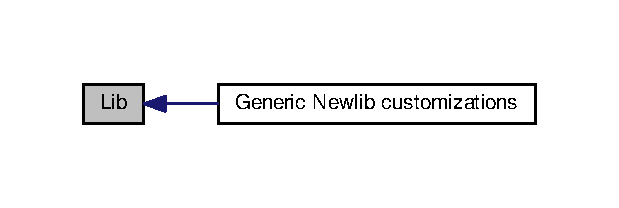
\includegraphics[width=297pt]{group__lib}
\end{center}
\end{figure}
\subsection*{Módulos}
\begin{DoxyCompactItemize}
\item 
\hyperlink{group__newlib}{Generic Newlib customizations}
\begin{DoxyCompactList}\small\item\em Library providing generic implementations of Newlib features for Contiki. \end{DoxyCompactList}\end{DoxyCompactItemize}


\subsection{Descrição detalhada}

\hypertarget{group__newlib}{\section{Generic Newlib customizations}
\label{group__newlib}\index{Generic Newlib customizations@{Generic Newlib customizations}}
}


Library providing generic implementations of Newlib features for Contiki.  


Diagrama de colaboração para Generic Newlib customizations\+:\nopagebreak
\begin{figure}[H]
\begin{center}
\leavevmode
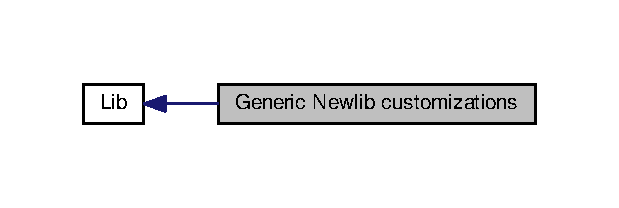
\includegraphics[width=297pt]{group__newlib}
\end{center}
\end{figure}
\subsection*{Ficheiros}
\begin{DoxyCompactItemize}
\item 
ficheiro \hyperlink{syscalls_8c}{syscalls.\+c}
\begin{DoxyCompactList}\small\item\em System calls. \end{DoxyCompactList}\end{DoxyCompactItemize}
\subsection*{Macros}
\begin{DoxyCompactItemize}
\item 
\hypertarget{group__newlib_gad72dbcf6d0153db1b8d8a58001feed83}{\#define {\bfseries D\+E\+B\+U\+G}~0}\label{group__newlib_gad72dbcf6d0153db1b8d8a58001feed83}

\item 
\hypertarget{group__newlib_ga1f464e950a4fa11e8821b5c725921a15}{\#define {\bfseries P\+R\+I\+N\+T\+F}(...)}\label{group__newlib_ga1f464e950a4fa11e8821b5c725921a15}

\end{DoxyCompactItemize}
\subsection*{Funções}
\begin{DoxyCompactItemize}
\item 
caddr\+\_\+t \hyperlink{group__newlib_gaae54d7b9578ba1fc171ce6f30f4c68a3}{\+\_\+sbrk} (int incr)
\begin{DoxyCompactList}\small\item\em Enlarges the allocated heap space. \end{DoxyCompactList}\end{DoxyCompactItemize}


\subsection{Descrição detalhada}
Library providing generic implementations of Newlib features for Contiki. 



\subsection{Documentação das funções}
\hypertarget{group__newlib_gaae54d7b9578ba1fc171ce6f30f4c68a3}{\index{Generic Newlib customizations@{Generic Newlib customizations}!\+\_\+sbrk@{\+\_\+sbrk}}
\index{\+\_\+sbrk@{\+\_\+sbrk}!Generic Newlib customizations@{Generic Newlib customizations}}
\subsubsection[{\+\_\+sbrk}]{\setlength{\rightskip}{0pt plus 5cm}caddr\+\_\+t \+\_\+sbrk (
\begin{DoxyParamCaption}
\item[{int}]{incr}
\end{DoxyParamCaption}
)}}\label{group__newlib_gaae54d7b9578ba1fc171ce6f30f4c68a3}


Enlarges the allocated heap space. 


\begin{DoxyParams}{Parâmetros}
{\em incr} & Number of bytes by which to increase the heap space \\
\hline
\end{DoxyParams}
\begin{DoxyReturn}{Retorna}
The previous end of heap on success (which is also a pointer to the start of the newly allocated memory if {\ttfamily incr} is positive), or {\ttfamily (caddr\+\_\+t)-\/1} with {\ttfamily errno} set to {\ttfamily E\+N\+O\+M\+E\+M} on error 
\end{DoxyReturn}

\begin{DoxyCode}
64 \{
65   \textcolor{comment}{/*}
66 \textcolor{comment}{   * Newlib's \_sbrk\_r() assumes that this global errno variable is used here,}
67 \textcolor{comment}{   * which is different from the errno definition provided by <errno.h>.}
68 \textcolor{comment}{   */}
69 \textcolor{preprocessor}{#undef errno}
70   \textcolor{keyword}{extern} \textcolor{keywordtype}{int} errno;
71 
72   \textcolor{comment}{/* Heap boundaries from linker script. */}
73   \textcolor{keyword}{extern} uint8\_t \_heap;
74   \textcolor{keyword}{extern} uint8\_t \_eheap;
75 
76   \textcolor{keyword}{static} uint8\_t *heap\_end = &\_heap;
77   uint8\_t *prev\_heap\_end = heap\_end;
78 
79   \textcolor{keywordflow}{if}(heap\_end + incr > &\_eheap) \{
80     PRINTF(\textcolor{stringliteral}{"Out of heap space!\(\backslash\)n"});
81     errno = ENOMEM;
82     \textcolor{keywordflow}{return} (caddr\_t)-1;
83   \}
84 
85   heap\_end += incr;
86   \textcolor{keywordflow}{return} (caddr\_t)prev\_heap\_end;
87 \}
\end{DoxyCode}

\hypertarget{group__MQTT__SN__DEBUG}{\section{M\+Q\+T\+T\+\_\+\+S\+N\+\_\+\+D\+E\+B\+U\+G}
\label{group__MQTT__SN__DEBUG}\index{M\+Q\+T\+T\+\_\+\+S\+N\+\_\+\+D\+E\+B\+U\+G@{M\+Q\+T\+T\+\_\+\+S\+N\+\_\+\+D\+E\+B\+U\+G}}
}
\subsection*{Macros}
\begin{DoxyCompactItemize}
\item 
\#define \hyperlink{group__MQTT__SN__DEBUG_ga7871b41b94f3b5aac9e79ad353903ae7}{D\+E\+B\+U\+G\+\_\+\+O\+S}
\begin{DoxyCompactList}\small\item\em Se definida habilita mensagens de debug da rede M\+Q\+T\+T-\/\+S\+N. \end{DoxyCompactList}\item 
\hypertarget{group__MQTT__SN__DEBUG_gac3a54f3a6ca71cb643dc99df536f503c}{\#define \hyperlink{group__MQTT__SN__DEBUG_gac3a54f3a6ca71cb643dc99df536f503c}{D\+E\+B\+U\+G\+\_\+\+T\+A\+S\+K}}\label{group__MQTT__SN__DEBUG_gac3a54f3a6ca71cb643dc99df536f503c}

\begin{DoxyCompactList}\small\item\em Se definida habilita mensagens de debug de tarefas da fila utilizada pelo M\+Q\+T\+T-\/\+S\+N. \end{DoxyCompactList}\end{DoxyCompactItemize}


\subsection{Descrição detalhada}
Macros de debug utilizadas para o M\+Q\+T\+T-\/\+S\+N 

\subsection{Documentação das macros}
\hypertarget{group__MQTT__SN__DEBUG_ga7871b41b94f3b5aac9e79ad353903ae7}{\index{M\+Q\+T\+T\+\_\+\+S\+N\+\_\+\+D\+E\+B\+U\+G@{M\+Q\+T\+T\+\_\+\+S\+N\+\_\+\+D\+E\+B\+U\+G}!D\+E\+B\+U\+G\+\_\+\+O\+S@{D\+E\+B\+U\+G\+\_\+\+O\+S}}
\index{D\+E\+B\+U\+G\+\_\+\+O\+S@{D\+E\+B\+U\+G\+\_\+\+O\+S}!M\+Q\+T\+T\+\_\+\+S\+N\+\_\+\+D\+E\+B\+U\+G@{M\+Q\+T\+T\+\_\+\+S\+N\+\_\+\+D\+E\+B\+U\+G}}
\subsubsection[{D\+E\+B\+U\+G\+\_\+\+O\+S}]{\setlength{\rightskip}{0pt plus 5cm}\#define D\+E\+B\+U\+G\+\_\+\+O\+S}}\label{group__MQTT__SN__DEBUG_ga7871b41b94f3b5aac9e79ad353903ae7}


Se definida habilita mensagens de debug da rede M\+Q\+T\+T-\/\+S\+N. 

Se definida habilita mensagens de debug do sistema operacional 
\hypertarget{group__MQTT__SN__CONTROL}{\section{M\+Q\+T\+T\+\_\+\+S\+N\+\_\+\+C\+O\+N\+T\+R\+O\+L}
\label{group__MQTT__SN__CONTROL}\index{M\+Q\+T\+T\+\_\+\+S\+N\+\_\+\+C\+O\+N\+T\+R\+O\+L@{M\+Q\+T\+T\+\_\+\+S\+N\+\_\+\+C\+O\+N\+T\+R\+O\+L}}
}
\subsection*{Macros}
\begin{DoxyCompactItemize}
\item 
\hypertarget{group__MQTT__SN__CONTROL_gac6620fe642df6fedae5da980e3cc1685}{\#define {\bfseries M\+Q\+T\+T\+\_\+\+S\+N\+\_\+\+M\+A\+X\+\_\+\+P\+A\+C\+K\+E\+T\+\_\+\+L\+E\+N\+G\+T\+H}~(255)}\label{group__MQTT__SN__CONTROL_gac6620fe642df6fedae5da980e3cc1685}

\item 
\hypertarget{group__MQTT__SN__CONTROL_ga3dccee9ebffc9265d5c3cd3107ca601b}{\#define {\bfseries M\+Q\+T\+T\+\_\+\+S\+N\+\_\+\+M\+A\+X\+\_\+\+T\+O\+P\+I\+C\+\_\+\+L\+E\+N\+G\+T\+H}~(M\+Q\+T\+T\+\_\+\+S\+N\+\_\+\+M\+A\+X\+\_\+\+P\+A\+C\+K\+E\+T\+\_\+\+L\+E\+N\+G\+T\+H-\/6)}\label{group__MQTT__SN__CONTROL_ga3dccee9ebffc9265d5c3cd3107ca601b}

\item 
\hypertarget{group__MQTT__SN__CONTROL_ga064185df38354c8d31cba8f173a8b39f}{\#define {\bfseries M\+Q\+T\+T\+\_\+\+S\+N\+\_\+\+T\+Y\+P\+E\+\_\+\+A\+D\+V\+E\+R\+T\+I\+S\+E}~(0x00)}\label{group__MQTT__SN__CONTROL_ga064185df38354c8d31cba8f173a8b39f}

\item 
\hypertarget{group__MQTT__SN__CONTROL_ga8170ee7211bec9249606010e8af4765d}{\#define {\bfseries M\+Q\+T\+T\+\_\+\+S\+N\+\_\+\+T\+Y\+P\+E\+\_\+\+S\+E\+A\+R\+C\+H\+G\+W}~(0x01)}\label{group__MQTT__SN__CONTROL_ga8170ee7211bec9249606010e8af4765d}

\item 
\hypertarget{group__MQTT__SN__CONTROL_ga5be35929c3e372b4a2fed0e133be0e92}{\#define {\bfseries M\+Q\+T\+T\+\_\+\+S\+N\+\_\+\+T\+Y\+P\+E\+\_\+\+G\+W\+I\+N\+F\+O}~(0x02)}\label{group__MQTT__SN__CONTROL_ga5be35929c3e372b4a2fed0e133be0e92}

\item 
\hypertarget{group__MQTT__SN__CONTROL_ga0ad512804838d2ba709e82ffb010d991}{\#define {\bfseries M\+Q\+T\+T\+\_\+\+S\+N\+\_\+\+T\+Y\+P\+E\+\_\+\+C\+O\+N\+N\+E\+C\+T}~(0x04)}\label{group__MQTT__SN__CONTROL_ga0ad512804838d2ba709e82ffb010d991}

\item 
\hypertarget{group__MQTT__SN__CONTROL_gac4469be7c31731176bfa8c5bd38f3a58}{\#define {\bfseries M\+Q\+T\+T\+\_\+\+S\+N\+\_\+\+T\+Y\+P\+E\+\_\+\+C\+O\+N\+N\+A\+C\+K}~(0x05)}\label{group__MQTT__SN__CONTROL_gac4469be7c31731176bfa8c5bd38f3a58}

\item 
\hypertarget{group__MQTT__SN__CONTROL_ga914fff9b2b9e7c08d6b732599f0cf348}{\#define {\bfseries M\+Q\+T\+T\+\_\+\+S\+N\+\_\+\+T\+Y\+P\+E\+\_\+\+W\+I\+L\+L\+T\+O\+P\+I\+C\+R\+E\+Q}~(0x06)}\label{group__MQTT__SN__CONTROL_ga914fff9b2b9e7c08d6b732599f0cf348}

\item 
\hypertarget{group__MQTT__SN__CONTROL_ga95c657f75f0f02a093b8623a50dc0af8}{\#define {\bfseries M\+Q\+T\+T\+\_\+\+S\+N\+\_\+\+T\+Y\+P\+E\+\_\+\+W\+I\+L\+L\+T\+O\+P\+I\+C}~(0x07)}\label{group__MQTT__SN__CONTROL_ga95c657f75f0f02a093b8623a50dc0af8}

\item 
\hypertarget{group__MQTT__SN__CONTROL_gaefa36203de4d9ff51372abd51fa6521a}{\#define {\bfseries M\+Q\+T\+T\+\_\+\+S\+N\+\_\+\+T\+Y\+P\+E\+\_\+\+W\+I\+L\+L\+M\+S\+G\+R\+E\+Q}~(0x08)}\label{group__MQTT__SN__CONTROL_gaefa36203de4d9ff51372abd51fa6521a}

\item 
\hypertarget{group__MQTT__SN__CONTROL_ga0ab12c9559a2419e1c88080fa3c594c0}{\#define {\bfseries M\+Q\+T\+T\+\_\+\+S\+N\+\_\+\+T\+Y\+P\+E\+\_\+\+W\+I\+L\+L\+M\+S\+G}~(0x09)}\label{group__MQTT__SN__CONTROL_ga0ab12c9559a2419e1c88080fa3c594c0}

\item 
\hypertarget{group__MQTT__SN__CONTROL_ga742472508835bbeab8a22d6294f34e8f}{\#define {\bfseries M\+Q\+T\+T\+\_\+\+S\+N\+\_\+\+T\+Y\+P\+E\+\_\+\+R\+E\+G\+I\+S\+T\+E\+R}~(0x0\+A)}\label{group__MQTT__SN__CONTROL_ga742472508835bbeab8a22d6294f34e8f}

\item 
\hypertarget{group__MQTT__SN__CONTROL_gab600be8ae75c06a49cc89d0f7255ac12}{\#define {\bfseries M\+Q\+T\+T\+\_\+\+S\+N\+\_\+\+T\+Y\+P\+E\+\_\+\+R\+E\+G\+A\+C\+K}~(0x0\+B)}\label{group__MQTT__SN__CONTROL_gab600be8ae75c06a49cc89d0f7255ac12}

\item 
\hypertarget{group__MQTT__SN__CONTROL_ga1c34c285be401165ca3b9ef1c9180354}{\#define {\bfseries M\+Q\+T\+T\+\_\+\+S\+N\+\_\+\+T\+Y\+P\+E\+\_\+\+P\+U\+B\+L\+I\+S\+H}~(0x0\+C)}\label{group__MQTT__SN__CONTROL_ga1c34c285be401165ca3b9ef1c9180354}

\item 
\hypertarget{group__MQTT__SN__CONTROL_ga5bc44c53d2905a5242a3b72d44c125b2}{\#define {\bfseries M\+Q\+T\+T\+\_\+\+S\+N\+\_\+\+T\+Y\+P\+E\+\_\+\+P\+U\+B\+A\+C\+K}~(0x0\+D)}\label{group__MQTT__SN__CONTROL_ga5bc44c53d2905a5242a3b72d44c125b2}

\item 
\hypertarget{group__MQTT__SN__CONTROL_gacef39c4b8c3dd36ed4caf90f6a716585}{\#define {\bfseries M\+Q\+T\+T\+\_\+\+S\+N\+\_\+\+T\+Y\+P\+E\+\_\+\+P\+U\+B\+C\+O\+M\+P}~(0x0\+E)}\label{group__MQTT__SN__CONTROL_gacef39c4b8c3dd36ed4caf90f6a716585}

\item 
\hypertarget{group__MQTT__SN__CONTROL_gac4953c83079abc9804fce7dca7b0a648}{\#define {\bfseries M\+Q\+T\+T\+\_\+\+S\+N\+\_\+\+T\+Y\+P\+E\+\_\+\+P\+U\+B\+R\+E\+C}~(0x0\+F)}\label{group__MQTT__SN__CONTROL_gac4953c83079abc9804fce7dca7b0a648}

\item 
\hypertarget{group__MQTT__SN__CONTROL_ga74daeb038d5cf996c680fc34b187dfba}{\#define {\bfseries M\+Q\+T\+T\+\_\+\+S\+N\+\_\+\+T\+Y\+P\+E\+\_\+\+P\+U\+B\+R\+E\+L}~(0x10)}\label{group__MQTT__SN__CONTROL_ga74daeb038d5cf996c680fc34b187dfba}

\item 
\hypertarget{group__MQTT__SN__CONTROL_ga1e4f5d7bc584d5ffcda760303ab76904}{\#define {\bfseries M\+Q\+T\+T\+\_\+\+S\+N\+\_\+\+T\+Y\+P\+E\+\_\+\+S\+U\+B\+S\+C\+R\+I\+B\+E}~(0x12)}\label{group__MQTT__SN__CONTROL_ga1e4f5d7bc584d5ffcda760303ab76904}

\item 
\hypertarget{group__MQTT__SN__CONTROL_ga6db4e874ad63924de121a89d4bcd559d}{\#define {\bfseries M\+Q\+T\+T\+\_\+\+S\+N\+\_\+\+T\+Y\+P\+E\+\_\+\+S\+U\+B\+A\+C\+K}~(0x13)}\label{group__MQTT__SN__CONTROL_ga6db4e874ad63924de121a89d4bcd559d}

\item 
\hypertarget{group__MQTT__SN__CONTROL_ga0aaddbe1b0ebd1ece45ada17e618e560}{\#define {\bfseries M\+Q\+T\+T\+\_\+\+S\+N\+\_\+\+T\+Y\+P\+E\+\_\+\+U\+N\+S\+U\+B\+S\+C\+R\+I\+B\+E}~(0x14)}\label{group__MQTT__SN__CONTROL_ga0aaddbe1b0ebd1ece45ada17e618e560}

\item 
\hypertarget{group__MQTT__SN__CONTROL_ga494ee75d7c290823f3738a4d77beea97}{\#define {\bfseries M\+Q\+T\+T\+\_\+\+S\+N\+\_\+\+T\+Y\+P\+E\+\_\+\+U\+N\+S\+U\+B\+A\+C\+K}~(0x15)}\label{group__MQTT__SN__CONTROL_ga494ee75d7c290823f3738a4d77beea97}

\item 
\hypertarget{group__MQTT__SN__CONTROL_ga24c4412f26f5db3dabc57c8511690a7b}{\#define {\bfseries M\+Q\+T\+T\+\_\+\+S\+N\+\_\+\+T\+Y\+P\+E\+\_\+\+P\+I\+N\+G\+R\+E\+Q}~(0x16)}\label{group__MQTT__SN__CONTROL_ga24c4412f26f5db3dabc57c8511690a7b}

\item 
\hypertarget{group__MQTT__SN__CONTROL_ga104849c06dad11e57805341ca6394513}{\#define {\bfseries M\+Q\+T\+T\+\_\+\+S\+N\+\_\+\+T\+Y\+P\+E\+\_\+\+P\+I\+N\+G\+R\+E\+S\+P}~(0x17)}\label{group__MQTT__SN__CONTROL_ga104849c06dad11e57805341ca6394513}

\item 
\hypertarget{group__MQTT__SN__CONTROL_gaeb18a759d020c1443a602636204c6fdd}{\#define {\bfseries M\+Q\+T\+T\+\_\+\+S\+N\+\_\+\+T\+Y\+P\+E\+\_\+\+D\+I\+S\+C\+O\+N\+N\+E\+C\+T}~(0x18)}\label{group__MQTT__SN__CONTROL_gaeb18a759d020c1443a602636204c6fdd}

\item 
\hypertarget{group__MQTT__SN__CONTROL_gae34bbdc05e79d37cc1f2060a885c3e05}{\#define {\bfseries M\+Q\+T\+T\+\_\+\+S\+N\+\_\+\+T\+Y\+P\+E\+\_\+\+W\+I\+L\+L\+T\+O\+P\+I\+C\+U\+P\+D}~(0x1\+A)}\label{group__MQTT__SN__CONTROL_gae34bbdc05e79d37cc1f2060a885c3e05}

\item 
\hypertarget{group__MQTT__SN__CONTROL_ga3181a18a9d476f1ca97a1bc935c8b712}{\#define {\bfseries M\+Q\+T\+T\+\_\+\+S\+N\+\_\+\+T\+Y\+P\+E\+\_\+\+W\+I\+L\+L\+T\+O\+P\+I\+C\+R\+E\+S\+P}~(0x1\+B)}\label{group__MQTT__SN__CONTROL_ga3181a18a9d476f1ca97a1bc935c8b712}

\item 
\hypertarget{group__MQTT__SN__CONTROL_ga63c970e654cb17f2a30294a719b11b71}{\#define {\bfseries M\+Q\+T\+T\+\_\+\+S\+N\+\_\+\+T\+Y\+P\+E\+\_\+\+W\+I\+L\+L\+M\+S\+G\+U\+P\+D}~(0x1\+C)}\label{group__MQTT__SN__CONTROL_ga63c970e654cb17f2a30294a719b11b71}

\item 
\hypertarget{group__MQTT__SN__CONTROL_ga855273768c5808acc67a07b8c4b6f5fa}{\#define {\bfseries M\+Q\+T\+T\+\_\+\+S\+N\+\_\+\+T\+Y\+P\+E\+\_\+\+W\+I\+L\+L\+M\+S\+G\+R\+E\+S\+P}~(0x1\+D)}\label{group__MQTT__SN__CONTROL_ga855273768c5808acc67a07b8c4b6f5fa}

\item 
\hypertarget{group__MQTT__SN__CONTROL_gaccc43fa2c1468ee81b07ca73265057e0}{\#define {\bfseries M\+Q\+T\+T\+\_\+\+S\+N\+\_\+\+T\+Y\+P\+E\+\_\+\+S\+U\+B\+\_\+\+W\+I\+L\+D\+C\+A\+R\+D}~(0x1\+E)}\label{group__MQTT__SN__CONTROL_gaccc43fa2c1468ee81b07ca73265057e0}

\item 
\hypertarget{group__MQTT__SN__CONTROL_ga206c51c6b01cdf9347809ebfc03caaef}{\#define {\bfseries M\+Q\+T\+T\+\_\+\+S\+N\+\_\+\+T\+O\+P\+I\+C\+\_\+\+T\+Y\+P\+E\+\_\+\+N\+O\+R\+M\+A\+L}~(0x00)}\label{group__MQTT__SN__CONTROL_ga206c51c6b01cdf9347809ebfc03caaef}

\item 
\hypertarget{group__MQTT__SN__CONTROL_ga206c51c6b01cdf9347809ebfc03caaef}{\#define {\bfseries M\+Q\+T\+T\+\_\+\+S\+N\+\_\+\+T\+O\+P\+I\+C\+\_\+\+T\+Y\+P\+E\+\_\+\+N\+O\+R\+M\+A\+L}~(0x00)}\label{group__MQTT__SN__CONTROL_ga206c51c6b01cdf9347809ebfc03caaef}

\item 
\hypertarget{group__MQTT__SN__CONTROL_ga655ae15e8e7734cedf42fab6eb3610b5}{\#define {\bfseries M\+Q\+T\+T\+\_\+\+S\+N\+\_\+\+T\+O\+P\+I\+C\+\_\+\+T\+Y\+P\+E\+\_\+\+P\+R\+E\+D\+E\+F\+I\+N\+E\+D}~(0x01)}\label{group__MQTT__SN__CONTROL_ga655ae15e8e7734cedf42fab6eb3610b5}

\item 
\hypertarget{group__MQTT__SN__CONTROL_ga655ae15e8e7734cedf42fab6eb3610b5}{\#define {\bfseries M\+Q\+T\+T\+\_\+\+S\+N\+\_\+\+T\+O\+P\+I\+C\+\_\+\+T\+Y\+P\+E\+\_\+\+P\+R\+E\+D\+E\+F\+I\+N\+E\+D}~(0x01)}\label{group__MQTT__SN__CONTROL_ga655ae15e8e7734cedf42fab6eb3610b5}

\item 
\hypertarget{group__MQTT__SN__CONTROL_gaa17c2076a81b61d2719199521563d1c5}{\#define {\bfseries M\+Q\+T\+T\+\_\+\+S\+N\+\_\+\+T\+O\+P\+I\+C\+\_\+\+T\+Y\+P\+E\+\_\+\+S\+H\+O\+R\+T}~(0x02)}\label{group__MQTT__SN__CONTROL_gaa17c2076a81b61d2719199521563d1c5}

\item 
\hypertarget{group__MQTT__SN__CONTROL_gaa17c2076a81b61d2719199521563d1c5}{\#define {\bfseries M\+Q\+T\+T\+\_\+\+S\+N\+\_\+\+T\+O\+P\+I\+C\+\_\+\+T\+Y\+P\+E\+\_\+\+S\+H\+O\+R\+T}~(0x02)}\label{group__MQTT__SN__CONTROL_gaa17c2076a81b61d2719199521563d1c5}

\item 
\hypertarget{group__MQTT__SN__CONTROL_ga2d49bf6469a7864f24a537f059ee0612}{\#define {\bfseries M\+Q\+T\+T\+\_\+\+S\+N\+\_\+\+F\+L\+A\+G\+\_\+\+D\+U\+P}~(0x1 $<$$<$ 7)}\label{group__MQTT__SN__CONTROL_ga2d49bf6469a7864f24a537f059ee0612}

\item 
\hypertarget{group__MQTT__SN__CONTROL_ga37b57822f47fbb4ba1639e5be988c437}{\#define {\bfseries M\+Q\+T\+T\+\_\+\+S\+N\+\_\+\+F\+L\+A\+G\+\_\+\+Q\+O\+S\+\_\+0}~(0x0 $<$$<$ 5)}\label{group__MQTT__SN__CONTROL_ga37b57822f47fbb4ba1639e5be988c437}

\item 
\hypertarget{group__MQTT__SN__CONTROL_ga6d04b90ba54b58e08caa593a84105f21}{\#define {\bfseries M\+Q\+T\+T\+\_\+\+S\+N\+\_\+\+F\+L\+A\+G\+\_\+\+Q\+O\+S\+\_\+1}~(0x1 $<$$<$ 5)}\label{group__MQTT__SN__CONTROL_ga6d04b90ba54b58e08caa593a84105f21}

\item 
\hypertarget{group__MQTT__SN__CONTROL_ga953eaf715ee6055e9f119950be8d7399}{\#define {\bfseries M\+Q\+T\+T\+\_\+\+S\+N\+\_\+\+F\+L\+A\+G\+\_\+\+Q\+O\+S\+\_\+2}~(0x2 $<$$<$ 5)}\label{group__MQTT__SN__CONTROL_ga953eaf715ee6055e9f119950be8d7399}

\item 
\hypertarget{group__MQTT__SN__CONTROL_ga8095eefa31299b606b4ba8bbbcb00195}{\#define {\bfseries M\+Q\+T\+T\+\_\+\+S\+N\+\_\+\+F\+L\+A\+G\+\_\+\+Q\+O\+S\+\_\+\+N1}~(0x3 $<$$<$ 5)}\label{group__MQTT__SN__CONTROL_ga8095eefa31299b606b4ba8bbbcb00195}

\item 
\hypertarget{group__MQTT__SN__CONTROL_ga45271b87fd548295bc4c86c225fc648e}{\#define {\bfseries M\+Q\+T\+T\+\_\+\+S\+N\+\_\+\+F\+L\+A\+G\+\_\+\+R\+E\+T\+A\+I\+N}~(0x1 $<$$<$ 4)}\label{group__MQTT__SN__CONTROL_ga45271b87fd548295bc4c86c225fc648e}

\item 
\hypertarget{group__MQTT__SN__CONTROL_ga8e3f7578e0fef59224e365cef8613f8e}{\#define {\bfseries M\+Q\+T\+T\+\_\+\+S\+N\+\_\+\+F\+L\+A\+G\+\_\+\+W\+I\+L\+L}~(0x1 $<$$<$ 3)}\label{group__MQTT__SN__CONTROL_ga8e3f7578e0fef59224e365cef8613f8e}

\item 
\hypertarget{group__MQTT__SN__CONTROL_ga842ab1c7124c0b63f62ed3283dafbe06}{\#define {\bfseries M\+Q\+T\+T\+\_\+\+S\+N\+\_\+\+F\+L\+A\+G\+\_\+\+C\+L\+E\+A\+N}~(0x1 $<$$<$ 2)}\label{group__MQTT__SN__CONTROL_ga842ab1c7124c0b63f62ed3283dafbe06}

\item 
\hypertarget{group__MQTT__SN__CONTROL_ga0066dd4afeef507b2e8f5ac01f71ea37}{\#define {\bfseries M\+Q\+T\+T\+\_\+\+S\+N\+\_\+\+P\+R\+O\+T\+O\+C\+O\+L\+\_\+\+I\+D}~(0x01)}\label{group__MQTT__SN__CONTROL_ga0066dd4afeef507b2e8f5ac01f71ea37}

\item 
\hypertarget{group__MQTT__SN__CONTROL_ga43005b6b1934800f67a6d169c779c92b}{\#define {\bfseries A\+C\+C\+E\+P\+T\+E\+D}~0x00}\label{group__MQTT__SN__CONTROL_ga43005b6b1934800f67a6d169c779c92b}

\item 
\hypertarget{group__MQTT__SN__CONTROL_ga9b2b214d1ddb0f617efdd26ccc91def4}{\#define {\bfseries R\+E\+J\+E\+C\+T\+E\+D\+\_\+\+C\+O\+N\+G\+E\+S\+T\+I\+O\+N}~0x01}\label{group__MQTT__SN__CONTROL_ga9b2b214d1ddb0f617efdd26ccc91def4}

\item 
\hypertarget{group__MQTT__SN__CONTROL_ga9b548f6c60530b07c9b9f5ef5b1ac8b9}{\#define {\bfseries R\+E\+J\+E\+C\+T\+E\+D\+\_\+\+I\+N\+V\+A\+L\+I\+D\+\_\+\+T\+O\+P\+I\+C\+\_\+\+I\+D}~0x02}\label{group__MQTT__SN__CONTROL_ga9b548f6c60530b07c9b9f5ef5b1ac8b9}

\item 
\hypertarget{group__MQTT__SN__CONTROL_ga93af4e6b658c4823ae9603b86bb7c64a}{\#define {\bfseries R\+E\+J\+E\+C\+T\+E\+D\+\_\+\+N\+O\+T\+\_\+\+S\+U\+P\+P\+O\+R\+T\+E\+D}~0x03}\label{group__MQTT__SN__CONTROL_ga93af4e6b658c4823ae9603b86bb7c64a}

\item 
\hypertarget{group__MQTT__SN__CONTROL_ga34bf6ae7cc029057c70910ae26a3335f}{\#define \hyperlink{group__MQTT__SN__CONTROL_ga34bf6ae7cc029057c70910ae26a3335f}{ss}(x)~sizeof(x)/sizeof($\ast$x)}\label{group__MQTT__SN__CONTROL_ga34bf6ae7cc029057c70910ae26a3335f}

\begin{DoxyCompactList}\small\item\em Computa o tamanho de um vetor de ponteiros. \end{DoxyCompactList}\item 
\hypertarget{group__MQTT__SN__CONTROL_ga8d316cee94174b8c2d16e328fdf1e607}{\#define \hyperlink{group__MQTT__SN__CONTROL_ga8d316cee94174b8c2d16e328fdf1e607}{M\+Q\+T\+T\+\_\+\+S\+N\+\_\+\+A\+U\+T\+O\+\_\+\+R\+E\+C\+O\+N\+N\+E\+C\+T}}\label{group__MQTT__SN__CONTROL_ga8d316cee94174b8c2d16e328fdf1e607}

\begin{DoxyCompactList}\small\item\em Define se o dispositivo deve se auto conectar de tempos em tempos. \end{DoxyCompactList}\item 
\hypertarget{group__MQTT__SN__CONTROL_ga180af20d177732dc470c147452feb30f}{\#define \hyperlink{group__MQTT__SN__CONTROL_ga180af20d177732dc470c147452feb30f}{M\+Q\+T\+T\+\_\+\+S\+N\+\_\+\+R\+E\+T\+R\+Y\+\_\+\+P\+I\+N\+G}~5}\label{group__MQTT__SN__CONTROL_ga180af20d177732dc470c147452feb30f}

\begin{DoxyCompactList}\small\item\em Número de tentativas de envio de P\+I\+N\+G R\+E\+Q\+U\+E\+S\+T antes de desconectar nó $<$-\/$>$ broker. \end{DoxyCompactList}\item 
\hypertarget{group__MQTT__SN__CONTROL_ga7533efb537d4d4eebf1b6d3d5256cb0b}{\#define \hyperlink{group__MQTT__SN__CONTROL_ga7533efb537d4d4eebf1b6d3d5256cb0b}{M\+Q\+T\+T\+\_\+\+S\+N\+\_\+\+T\+I\+M\+E\+O\+U\+T\+\_\+\+C\+O\+N\+N\+E\+C\+T}~9$\ast$C\+L\+O\+C\+K\+\_\+\+S\+E\+C\+O\+N\+D}\label{group__MQTT__SN__CONTROL_ga7533efb537d4d4eebf1b6d3d5256cb0b}

\begin{DoxyCompactList}\small\item\em Tempo base para comunicação M\+Q\+T\+T-\/\+S\+N broker $<$-\/$>$ nó \end{DoxyCompactList}\item 
\hypertarget{group__MQTT__SN__CONTROL_ga47da8d46176b160b0db00fe221725d4c}{\#define \hyperlink{group__MQTT__SN__CONTROL_ga47da8d46176b160b0db00fe221725d4c}{M\+Q\+T\+T\+\_\+\+S\+N\+\_\+\+T\+I\+M\+E\+O\+U\+T}~C\+L\+O\+C\+K\+\_\+\+S\+E\+C\+O\+N\+D}\label{group__MQTT__SN__CONTROL_ga47da8d46176b160b0db00fe221725d4c}

\begin{DoxyCompactList}\small\item\em Tempo base para comunicação M\+Q\+T\+T-\/\+S\+N broker $<$-\/$>$ nó \end{DoxyCompactList}\item 
\hypertarget{group__MQTT__SN__CONTROL_gaad5ac7de3008d8fa37447193aebc31e2}{\#define \hyperlink{group__MQTT__SN__CONTROL_gaad5ac7de3008d8fa37447193aebc31e2}{M\+Q\+T\+T\+\_\+\+S\+N\+\_\+\+R\+E\+T\+R\+Y}~5}\label{group__MQTT__SN__CONTROL_gaad5ac7de3008d8fa37447193aebc31e2}

\begin{DoxyCompactList}\small\item\em Número de tentativas de enviar qualquer pacote ao broker antes de desconectar. \end{DoxyCompactList}\item 
\hypertarget{group__MQTT__SN__CONTROL_ga45ab5881e190d570f3784e50be2cce65}{\#define \hyperlink{group__MQTT__SN__CONTROL_ga45ab5881e190d570f3784e50be2cce65}{M\+A\+X\+\_\+\+Q\+U\+E\+U\+E\+\_\+\+M\+Q\+T\+T\+\_\+\+S\+N}~100}\label{group__MQTT__SN__CONTROL_ga45ab5881e190d570f3784e50be2cce65}

\begin{DoxyCompactList}\small\item\em Número máximo de tarefas a serem inseridas alocadas dinamicamente M\+Q\+T\+T-\/\+S\+N. \end{DoxyCompactList}\item 
\hypertarget{group__MQTT__SN__CONTROL_ga5ed98e8fc00194886ebc14d25540f81b}{\#define \hyperlink{group__MQTT__SN__CONTROL_ga5ed98e8fc00194886ebc14d25540f81b}{M\+A\+X\+\_\+\+T\+O\+P\+I\+C\+\_\+\+U\+S\+E\+D}~100}\label{group__MQTT__SN__CONTROL_ga5ed98e8fc00194886ebc14d25540f81b}

\begin{DoxyCompactList}\small\item\em Número máximo de tópicos que o usuário pode registrar, a A\+P\+I cria um conjunto de estruturas para o bind de topic e short topic id. \end{DoxyCompactList}\end{DoxyCompactItemize}


\subsection{Descrição detalhada}
Macros de protocolos utilizadas para o M\+Q\+T\+T-\/\+S\+N

Macros de controle utilizadas para o M\+Q\+T\+T-\/\+S\+N 
\hypertarget{group__Pacotes}{\section{Pacotes}
\label{group__Pacotes}\index{Pacotes@{Pacotes}}
}
\subsection*{Estruturas de Dados}
\begin{DoxyCompactItemize}
\item 
struct \hyperlink{structdisconnect__packet__t}{disconnect\+\_\+packet\+\_\+t}
\begin{DoxyCompactList}\small\item\em Estrutura de pacote de desconexão do broker M\+Q\+T\+T-\/\+S\+N. \end{DoxyCompactList}\item 
struct \hyperlink{structping__req__t}{ping\+\_\+req\+\_\+t}
\begin{DoxyCompactList}\small\item\em Estrutura de pacote de desconexão do broker M\+Q\+T\+T-\/\+S\+N. \end{DoxyCompactList}\item 
struct \hyperlink{structpublish__packet__t}{publish\+\_\+packet\+\_\+t}
\begin{DoxyCompactList}\small\item\em Estrutura de pacote de publicação M\+Q\+T\+T-\/\+S\+N. \end{DoxyCompactList}\item 
struct \hyperlink{structsubscribe__wildcard__packet__t}{subscribe\+\_\+wildcard\+\_\+packet\+\_\+t}
\begin{DoxyCompactList}\small\item\em Estrutura de pacote de inscrição do tipo Wildcard M\+Q\+T\+T-\/\+S\+N. \end{DoxyCompactList}\item 
struct \hyperlink{structsubscribe__packet__t}{subscribe\+\_\+packet\+\_\+t}
\begin{DoxyCompactList}\small\item\em Estrutura de pacote M\+Q\+T\+T-\/\+S\+N do tipo S\+U\+B\+S\+C\+R\+I\+B\+E. \end{DoxyCompactList}\item 
struct \hyperlink{structconnect__packet__t}{connect\+\_\+packet\+\_\+t}
\begin{DoxyCompactList}\small\item\em Estrutura de pacotes M\+Q\+T\+T-\/\+S\+N do tipo C\+O\+N\+N\+E\+C\+T. \end{DoxyCompactList}\item 
struct \hyperlink{structregister__packet__t}{register\+\_\+packet\+\_\+t}
\begin{DoxyCompactList}\small\item\em Estrutura de pacotes M\+Q\+T\+T-\/\+S\+N do tipo R\+E\+G\+I\+S\+T\+E\+R. \end{DoxyCompactList}\item 
struct \hyperlink{structwilltopic__packet__t}{willtopic\+\_\+packet\+\_\+t}
\begin{DoxyCompactList}\small\item\em Estrutura de pacotes M\+Q\+T\+T-\/\+S\+N do tipo W\+I\+L\+L T\+O\+P\+I\+C. \end{DoxyCompactList}\item 
struct \hyperlink{structwillmessage__packet__t}{willmessage\+\_\+packet\+\_\+t}
\begin{DoxyCompactList}\small\item\em Estrutura de pacotes M\+Q\+T\+T-\/\+S\+N do tipo W\+I\+L\+L M\+E\+S\+S\+A\+G\+E. \end{DoxyCompactList}\item 
struct \hyperlink{structregack__packet__t}{regack\+\_\+packet\+\_\+t}
\begin{DoxyCompactList}\small\item\em Estrutura de pacotes M\+Q\+T\+T-\/\+S\+N do tipo R\+E\+G\+A\+C\+K. \end{DoxyCompactList}\end{DoxyCompactItemize}
\subsection*{Funções}
\begin{DoxyCompactItemize}
\item 
\hypertarget{group__Pacotes_gab898071398b359603a35c202e9c65f3b}{struct {\bfseries \+\_\+\+\_\+attribute\+\_\+\+\_\+} ((packed))}\label{group__Pacotes_gab898071398b359603a35c202e9c65f3b}

\end{DoxyCompactItemize}
\subsection*{Variáveis}
\begin{DoxyCompactItemize}
\item 
\hypertarget{group__Pacotes_ga1bdd22cd8ef2662e484e03ebdae7c970}{{\bfseries disconnect\+\_\+packet\+\_\+t}}\label{group__Pacotes_ga1bdd22cd8ef2662e484e03ebdae7c970}

\item 
\hypertarget{group__Pacotes_gaaa5b26ddb66cc7e85a9f4b30881775f2}{{\bfseries ping\+\_\+req\+\_\+t}}\label{group__Pacotes_gaaa5b26ddb66cc7e85a9f4b30881775f2}

\item 
\hypertarget{group__Pacotes_ga1f5bdda25ae963bb270e8a301b201b51}{{\bfseries publish\+\_\+packet\+\_\+t}}\label{group__Pacotes_ga1f5bdda25ae963bb270e8a301b201b51}

\item 
\hypertarget{group__Pacotes_gad20a7c29debd43f1bb693ea71cf25f37}{{\bfseries subscribe\+\_\+wildcard\+\_\+packet\+\_\+t}}\label{group__Pacotes_gad20a7c29debd43f1bb693ea71cf25f37}

\item 
\hypertarget{group__Pacotes_gad1653d1eb1e0b157ee553f5e18e837e3}{{\bfseries subscribe\+\_\+packet\+\_\+t}}\label{group__Pacotes_gad1653d1eb1e0b157ee553f5e18e837e3}

\item 
\hypertarget{group__Pacotes_gac7e9bb2727332431de0ed82739b64a37}{{\bfseries connect\+\_\+packet\+\_\+t}}\label{group__Pacotes_gac7e9bb2727332431de0ed82739b64a37}

\item 
\hypertarget{group__Pacotes_ga504f9ba055b5a5a51a852c85ba691d2f}{{\bfseries register\+\_\+packet\+\_\+t}}\label{group__Pacotes_ga504f9ba055b5a5a51a852c85ba691d2f}

\item 
\hypertarget{group__Pacotes_ga10d9b05d37a49ef4473051eb8cd9062e}{{\bfseries willtopic\+\_\+packet\+\_\+t}}\label{group__Pacotes_ga10d9b05d37a49ef4473051eb8cd9062e}

\item 
\hypertarget{group__Pacotes_ga498ec637bb31754407eaf35a3c0b3b4b}{{\bfseries willmessage\+\_\+packet\+\_\+t}}\label{group__Pacotes_ga498ec637bb31754407eaf35a3c0b3b4b}

\item 
\hypertarget{group__Pacotes_ga35c8d1d4849e06b6cd1a59b1d86b8368}{{\bfseries regack\+\_\+packet\+\_\+t}}\label{group__Pacotes_ga35c8d1d4849e06b6cd1a59b1d86b8368}

\end{DoxyCompactItemize}


\subsection{Descrição detalhada}
Macros de debug utilizadas para o M\+Q\+T\+T-\/\+S\+N 
\chapter{Documentação da classe}
\hypertarget{structconnect__packet__t}{\section{Referência à estrutura connect\+\_\+packet\+\_\+t}
\label{structconnect__packet__t}\index{connect\+\_\+packet\+\_\+t@{connect\+\_\+packet\+\_\+t}}
}


Estrutura de pacotes M\+Q\+T\+T-\/\+S\+N do tipo C\+O\+N\+N\+E\+C\+T.  




{\ttfamily \#include $<$mqtt\+\_\+sn.\+h$>$}



\subsection{Descrição detalhada}
Estrutura de pacotes M\+Q\+T\+T-\/\+S\+N do tipo C\+O\+N\+N\+E\+C\+T. 

A documentação para esta estrutura foi gerada a partir do seguinte ficheiro\+:\begin{DoxyCompactItemize}
\item 
\hyperlink{mqtt__sn_8h}{mqtt\+\_\+sn.\+h}\end{DoxyCompactItemize}

\hypertarget{structdisconnect__packet__t}{\section{Referência à estrutura disconnect\+\_\+packet\+\_\+t}
\label{structdisconnect__packet__t}\index{disconnect\+\_\+packet\+\_\+t@{disconnect\+\_\+packet\+\_\+t}}
}


Estrutura de pacote de desconexão do broker M\+Q\+T\+T-\/\+S\+N.  




{\ttfamily \#include $<$mqtt\+\_\+sn.\+h$>$}



\subsection{Descrição detalhada}
Estrutura de pacote de desconexão do broker M\+Q\+T\+T-\/\+S\+N. 

A documentação para esta estrutura foi gerada a partir do seguinte ficheiro\+:\begin{DoxyCompactItemize}
\item 
\hyperlink{mqtt__sn_8h}{mqtt\+\_\+sn.\+h}\end{DoxyCompactItemize}

\hypertarget{structmqtt__sn__con__t}{\section{Referência à estrutura mqtt\+\_\+sn\+\_\+con\+\_\+t}
\label{structmqtt__sn__con__t}\index{mqtt\+\_\+sn\+\_\+con\+\_\+t@{mqtt\+\_\+sn\+\_\+con\+\_\+t}}
}


Estrutura de conexão ao broker M\+Q\+T\+T-\/\+S\+N.  




{\ttfamily \#include $<$mqtt\+\_\+sn.\+h$>$}

\subsection*{Campos de Dados}
\begin{DoxyCompactItemize}
\item 
\hypertarget{structmqtt__sn__con__t_a60158486bd2056b682241cd713f462ac}{struct simple\+\_\+udp\+\_\+connection {\bfseries udp\+\_\+con}}\label{structmqtt__sn__con__t_a60158486bd2056b682241cd713f462ac}

\item 
\hypertarget{structmqtt__sn__con__t_ae3c6408a5f3fb41bcddcf7e8266f41a6}{uint16\+\_\+t \hyperlink{structmqtt__sn__con__t_ae3c6408a5f3fb41bcddcf7e8266f41a6}{udp\+\_\+port}}\label{structmqtt__sn__con__t_ae3c6408a5f3fb41bcddcf7e8266f41a6}

\begin{DoxyCompactList}\small\item\em Porta U\+D\+P de conexão com o broker (default\+:1884) \end{DoxyCompactList}\item 
\hypertarget{structmqtt__sn__con__t_a058796ada31936dced646e5da3eb329a}{uint16\+\_\+t $\ast$ \hyperlink{structmqtt__sn__con__t_a058796ada31936dced646e5da3eb329a}{ipv6\+\_\+broker}}\label{structmqtt__sn__con__t_a058796ada31936dced646e5da3eb329a}

\begin{DoxyCompactList}\small\item\em Endereço I\+Pv6 do broker U\+D\+P. \end{DoxyCompactList}\item 
\hypertarget{structmqtt__sn__con__t_a276b967ec5d6e3305ee4695488e4472b}{uint8\+\_\+t \hyperlink{structmqtt__sn__con__t_a276b967ec5d6e3305ee4695488e4472b}{keep\+\_\+alive}}\label{structmqtt__sn__con__t_a276b967ec5d6e3305ee4695488e4472b}

\begin{DoxyCompactList}\small\item\em Tempo de requisição Keep Alive para P\+I\+N\+G\+R\+E\+Q e P\+I\+N\+G\+R\+E\+S\+P. \end{DoxyCompactList}\item 
\hypertarget{structmqtt__sn__con__t_a3880622ca383fee22fbbac18442bae32}{const char $\ast$ \hyperlink{structmqtt__sn__con__t_a3880622ca383fee22fbbac18442bae32}{client\+\_\+id}}\label{structmqtt__sn__con__t_a3880622ca383fee22fbbac18442bae32}

\begin{DoxyCompactList}\small\item\em Identificador de cliente para conexão com o broker M\+Q\+T\+T-\/\+S\+N. \end{DoxyCompactList}\item 
\hypertarget{structmqtt__sn__con__t_a23561785b3c6cff4ce4bdb8c1a75b571}{char $\ast$ {\bfseries will\+\_\+topic}}\label{structmqtt__sn__con__t_a23561785b3c6cff4ce4bdb8c1a75b571}

\item 
\hypertarget{structmqtt__sn__con__t_a70c7f56bdf5d7086550c75ac8bc98a08}{char $\ast$ {\bfseries will\+\_\+message}}\label{structmqtt__sn__con__t_a70c7f56bdf5d7086550c75ac8bc98a08}

\end{DoxyCompactItemize}


\subsection{Descrição detalhada}
Estrutura de conexão ao broker M\+Q\+T\+T-\/\+S\+N. 

A documentação para esta estrutura foi gerada a partir do seguinte ficheiro\+:\begin{DoxyCompactItemize}
\item 
\hyperlink{mqtt__sn_8h}{mqtt\+\_\+sn.\+h}\end{DoxyCompactItemize}

\hypertarget{structmqtt__sn__task__t}{\section{Referência à estrutura mqtt\+\_\+sn\+\_\+task\+\_\+t}
\label{structmqtt__sn__task__t}\index{mqtt\+\_\+sn\+\_\+task\+\_\+t@{mqtt\+\_\+sn\+\_\+task\+\_\+t}}
}


Estrutura de tarefa de fila M\+Q\+T\+T-\/\+S\+N.  




{\ttfamily \#include $<$mqtt\+\_\+sn.\+h$>$}

\subsection*{Campos de Dados}
\begin{DoxyCompactItemize}
\item 
\hypertarget{structmqtt__sn__task__t_afb14d280d486f10af744fb1ac7f145eb}{uint8\+\_\+t \hyperlink{structmqtt__sn__task__t_afb14d280d486f10af744fb1ac7f145eb}{msg\+\_\+type\+\_\+q}}\label{structmqtt__sn__task__t_afb14d280d486f10af744fb1ac7f145eb}

\begin{DoxyCompactList}\small\item\em Tipo de mensagem a ser alocada. \end{DoxyCompactList}\item 
\hypertarget{structmqtt__sn__task__t_a25bc8ea535927589bca3720e0e838958}{uint8\+\_\+t \hyperlink{structmqtt__sn__task__t_a25bc8ea535927589bca3720e0e838958}{short\+\_\+topic}}\label{structmqtt__sn__task__t_a25bc8ea535927589bca3720e0e838958}

\begin{DoxyCompactList}\small\item\em Tópico curto ou topic id a ser publicado/inscrito. \end{DoxyCompactList}\item 
\hypertarget{structmqtt__sn__task__t_a1dba79ab8685a56d3ae57d84aca21ce8}{uint16\+\_\+t \hyperlink{structmqtt__sn__task__t_a1dba79ab8685a56d3ae57d84aca21ce8}{id\+\_\+task}}\label{structmqtt__sn__task__t_a1dba79ab8685a56d3ae57d84aca21ce8}

\begin{DoxyCompactList}\small\item\em Identificador da tarefa. \end{DoxyCompactList}\item 
\hypertarget{structmqtt__sn__task__t_a5ce109928f26d01872230443c75c91f8}{uint8\+\_\+t \hyperlink{structmqtt__sn__task__t_a5ce109928f26d01872230443c75c91f8}{qos\+\_\+level}}\label{structmqtt__sn__task__t_a5ce109928f26d01872230443c75c91f8}

\begin{DoxyCompactList}\small\item\em Nível Qo\+S da tarefa a ser alocada na pilha. \end{DoxyCompactList}\item 
\hypertarget{structmqtt__sn__task__t_ae25d47ab22bd975ad97012eddb6bbfce}{uint8\+\_\+t {\bfseries retain}}\label{structmqtt__sn__task__t_ae25d47ab22bd975ad97012eddb6bbfce}

\end{DoxyCompactItemize}


\subsection{Descrição detalhada}
Estrutura de tarefa de fila M\+Q\+T\+T-\/\+S\+N. 

A documentação para esta estrutura foi gerada a partir do seguinte ficheiro\+:\begin{DoxyCompactItemize}
\item 
\hyperlink{mqtt__sn_8h}{mqtt\+\_\+sn.\+h}\end{DoxyCompactItemize}

\hypertarget{structnode}{\section{Referência à estrutura node}
\label{structnode}\index{node@{node}}
}


Estrutura de fila M\+Q\+T\+T-\/\+S\+N.  




{\ttfamily \#include $<$mqtt\+\_\+sn.\+h$>$}



Diagrama de colaboração para node\+:\nopagebreak
\begin{figure}[H]
\begin{center}
\leavevmode
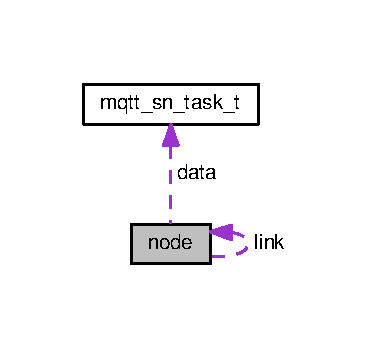
\includegraphics[width=178pt]{structnode__coll__graph}
\end{center}
\end{figure}
\subsection*{Campos de Dados}
\begin{DoxyCompactItemize}
\item 
\hypertarget{structnode_a2a4aa9e422389a8d7a97309a99143ce2}{\hyperlink{structmqtt__sn__task__t}{mqtt\+\_\+sn\+\_\+task\+\_\+t} {\bfseries data}}\label{structnode_a2a4aa9e422389a8d7a97309a99143ce2}

\item 
\hypertarget{structnode_ae20eb3a9a05750fd84dd04b48a8940c3}{struct \hyperlink{structnode}{node} $\ast$ {\bfseries link}}\label{structnode_ae20eb3a9a05750fd84dd04b48a8940c3}

\end{DoxyCompactItemize}


\subsection{Descrição detalhada}
Estrutura de fila M\+Q\+T\+T-\/\+S\+N. 

A documentação para esta estrutura foi gerada a partir do seguinte ficheiro\+:\begin{DoxyCompactItemize}
\item 
\hyperlink{mqtt__sn_8h}{mqtt\+\_\+sn.\+h}\end{DoxyCompactItemize}

\hypertarget{structping__req__t}{\section{Referência à estrutura ping\+\_\+req\+\_\+t}
\label{structping__req__t}\index{ping\+\_\+req\+\_\+t@{ping\+\_\+req\+\_\+t}}
}


Estrutura de pacote de desconexão do broker M\+Q\+T\+T-\/\+S\+N.  




{\ttfamily \#include $<$mqtt\+\_\+sn.\+h$>$}



\subsection{Descrição detalhada}
Estrutura de pacote de desconexão do broker M\+Q\+T\+T-\/\+S\+N. 

A documentação para esta estrutura foi gerada a partir do seguinte ficheiro\+:\begin{DoxyCompactItemize}
\item 
\hyperlink{mqtt__sn_8h}{mqtt\+\_\+sn.\+h}\end{DoxyCompactItemize}

\hypertarget{structpublish__packet__t}{\section{Referência à estrutura publish\+\_\+packet\+\_\+t}
\label{structpublish__packet__t}\index{publish\+\_\+packet\+\_\+t@{publish\+\_\+packet\+\_\+t}}
}


Estrutura de pacote de publicação M\+Q\+T\+T-\/\+S\+N.  




{\ttfamily \#include $<$mqtt\+\_\+sn.\+h$>$}



\subsection{Descrição detalhada}
Estrutura de pacote de publicação M\+Q\+T\+T-\/\+S\+N. 

A documentação para esta estrutura foi gerada a partir do seguinte ficheiro\+:\begin{DoxyCompactItemize}
\item 
\hyperlink{mqtt__sn_8h}{mqtt\+\_\+sn.\+h}\end{DoxyCompactItemize}

\hypertarget{structregack__packet__t}{\section{Referência à estrutura regack\+\_\+packet\+\_\+t}
\label{structregack__packet__t}\index{regack\+\_\+packet\+\_\+t@{regack\+\_\+packet\+\_\+t}}
}


Estrutura de pacotes M\+Q\+T\+T-\/\+S\+N do tipo R\+E\+G\+A\+C\+K.  




{\ttfamily \#include $<$mqtt\+\_\+sn.\+h$>$}



\subsection{Descrição detalhada}
Estrutura de pacotes M\+Q\+T\+T-\/\+S\+N do tipo R\+E\+G\+A\+C\+K. 

A documentação para esta estrutura foi gerada a partir do seguinte ficheiro\+:\begin{DoxyCompactItemize}
\item 
\hyperlink{mqtt__sn_8h}{mqtt\+\_\+sn.\+h}\end{DoxyCompactItemize}

\hypertarget{structregister__packet__t}{\section{Referência à estrutura register\+\_\+packet\+\_\+t}
\label{structregister__packet__t}\index{register\+\_\+packet\+\_\+t@{register\+\_\+packet\+\_\+t}}
}


Estrutura de pacotes M\+Q\+T\+T-\/\+S\+N do tipo R\+E\+G\+I\+S\+T\+E\+R.  




{\ttfamily \#include $<$mqtt\+\_\+sn.\+h$>$}



\subsection{Descrição detalhada}
Estrutura de pacotes M\+Q\+T\+T-\/\+S\+N do tipo R\+E\+G\+I\+S\+T\+E\+R. 

A documentação para esta estrutura foi gerada a partir do seguinte ficheiro\+:\begin{DoxyCompactItemize}
\item 
\hyperlink{mqtt__sn_8h}{mqtt\+\_\+sn.\+h}\end{DoxyCompactItemize}

\hypertarget{structshort__topics__t}{\section{Referência à estrutura short\+\_\+topics\+\_\+t}
\label{structshort__topics__t}\index{short\+\_\+topics\+\_\+t@{short\+\_\+topics\+\_\+t}}
}
\subsection*{Campos de Dados}
\begin{DoxyCompactItemize}
\item 
\hypertarget{structshort__topics__t_a0f942951500293608a04b92a49df4f69}{char $\ast$ {\bfseries topic\+\_\+name}}\label{structshort__topics__t_a0f942951500293608a04b92a49df4f69}

\item 
\hypertarget{structshort__topics__t_aa0a77b0dbcddeb15cfc004d18a9a093a}{uint8\+\_\+t {\bfseries short\+\_\+topic\+\_\+id}}\label{structshort__topics__t_aa0a77b0dbcddeb15cfc004d18a9a093a}

\item 
\hypertarget{structshort__topics__t_aa508bc242f4e53ea59cf936e8072aa2d}{uint8\+\_\+t {\bfseries subscribed}}\label{structshort__topics__t_aa508bc242f4e53ea59cf936e8072aa2d}

\end{DoxyCompactItemize}


A documentação para esta estrutura foi gerada a partir do seguinte ficheiro\+:\begin{DoxyCompactItemize}
\item 
\hyperlink{mqtt__sn_8h}{mqtt\+\_\+sn.\+h}\end{DoxyCompactItemize}

\hypertarget{structsubscribe__packet__t}{\section{Referência à estrutura subscribe\+\_\+packet\+\_\+t}
\label{structsubscribe__packet__t}\index{subscribe\+\_\+packet\+\_\+t@{subscribe\+\_\+packet\+\_\+t}}
}


Estrutura de pacote M\+Q\+T\+T-\/\+S\+N do tipo S\+U\+B\+S\+C\+R\+I\+B\+E.  




{\ttfamily \#include $<$mqtt\+\_\+sn.\+h$>$}



\subsection{Descrição detalhada}
Estrutura de pacote M\+Q\+T\+T-\/\+S\+N do tipo S\+U\+B\+S\+C\+R\+I\+B\+E. 

A documentação para esta estrutura foi gerada a partir do seguinte ficheiro\+:\begin{DoxyCompactItemize}
\item 
\hyperlink{mqtt__sn_8h}{mqtt\+\_\+sn.\+h}\end{DoxyCompactItemize}

\hypertarget{structsubscribe__wildcard__packet__t}{\section{Referência à estrutura subscribe\+\_\+wildcard\+\_\+packet\+\_\+t}
\label{structsubscribe__wildcard__packet__t}\index{subscribe\+\_\+wildcard\+\_\+packet\+\_\+t@{subscribe\+\_\+wildcard\+\_\+packet\+\_\+t}}
}


Estrutura de pacote de inscrição do tipo Wildcard M\+Q\+T\+T-\/\+S\+N.  




{\ttfamily \#include $<$mqtt\+\_\+sn.\+h$>$}



\subsection{Descrição detalhada}
Estrutura de pacote de inscrição do tipo Wildcard M\+Q\+T\+T-\/\+S\+N. 

A documentação para esta estrutura foi gerada a partir do seguinte ficheiro\+:\begin{DoxyCompactItemize}
\item 
\hyperlink{mqtt__sn_8h}{mqtt\+\_\+sn.\+h}\end{DoxyCompactItemize}

\hypertarget{structwillmessage__packet__t}{\section{Referência à estrutura willmessage\+\_\+packet\+\_\+t}
\label{structwillmessage__packet__t}\index{willmessage\+\_\+packet\+\_\+t@{willmessage\+\_\+packet\+\_\+t}}
}


Estrutura de pacotes M\+Q\+T\+T-\/\+S\+N do tipo W\+I\+L\+L M\+E\+S\+S\+A\+G\+E.  




{\ttfamily \#include $<$mqtt\+\_\+sn.\+h$>$}



\subsection{Descrição detalhada}
Estrutura de pacotes M\+Q\+T\+T-\/\+S\+N do tipo W\+I\+L\+L M\+E\+S\+S\+A\+G\+E. 

A documentação para esta estrutura foi gerada a partir do seguinte ficheiro\+:\begin{DoxyCompactItemize}
\item 
\hyperlink{mqtt__sn_8h}{mqtt\+\_\+sn.\+h}\end{DoxyCompactItemize}

\hypertarget{structwilltopic__packet__t}{\section{Referência à estrutura willtopic\+\_\+packet\+\_\+t}
\label{structwilltopic__packet__t}\index{willtopic\+\_\+packet\+\_\+t@{willtopic\+\_\+packet\+\_\+t}}
}


Estrutura de pacotes M\+Q\+T\+T-\/\+S\+N do tipo W\+I\+L\+L T\+O\+P\+I\+C.  




{\ttfamily \#include $<$mqtt\+\_\+sn.\+h$>$}



\subsection{Descrição detalhada}
Estrutura de pacotes M\+Q\+T\+T-\/\+S\+N do tipo W\+I\+L\+L T\+O\+P\+I\+C. 

A documentação para esta estrutura foi gerada a partir do seguinte ficheiro\+:\begin{DoxyCompactItemize}
\item 
\hyperlink{mqtt__sn_8h}{mqtt\+\_\+sn.\+h}\end{DoxyCompactItemize}

\chapter{Documentação do ficheiro}
\hypertarget{main__core_8c}{\section{Referência ao ficheiro main\+\_\+core.\+c}
\label{main__core_8c}\index{main\+\_\+core.\+c@{main\+\_\+core.\+c}}
}


Arquivo principal do porte do M\+Q\+T\+T-\/\+S\+N, utilizado para testar.  


{\ttfamily \#include \char`\"{}contiki.\+h\char`\"{}}\\*
{\ttfamily \#include \char`\"{}lib/random.\+h\char`\"{}}\\*
{\ttfamily \#include \char`\"{}clock.\+h\char`\"{}}\\*
{\ttfamily \#include \char`\"{}sys/ctimer.\+h\char`\"{}}\\*
{\ttfamily \#include \char`\"{}net/ip/uip.\+h\char`\"{}}\\*
{\ttfamily \#include \char`\"{}net/ipv6/uip-\/ds6.\+h\char`\"{}}\\*
{\ttfamily \#include \char`\"{}mqtt\+\_\+sn.\+h\char`\"{}}\\*
{\ttfamily \#include \char`\"{}dev/leds.\+h\char`\"{}}\\*
{\ttfamily \#include \char`\"{}net/rime/rime.\+h\char`\"{}}\\*
{\ttfamily \#include \char`\"{}simple-\/udp.\+h\char`\"{}}\\*
{\ttfamily \#include $<$stdio.\+h$>$}\\*
{\ttfamily \#include $<$string.\+h$>$}\\*
{\ttfamily \#include $<$stdlib.\+h$>$}\\*
Diagrama de dependências de inclusão para main\+\_\+core.\+c\+:\nopagebreak
\begin{figure}[H]
\begin{center}
\leavevmode
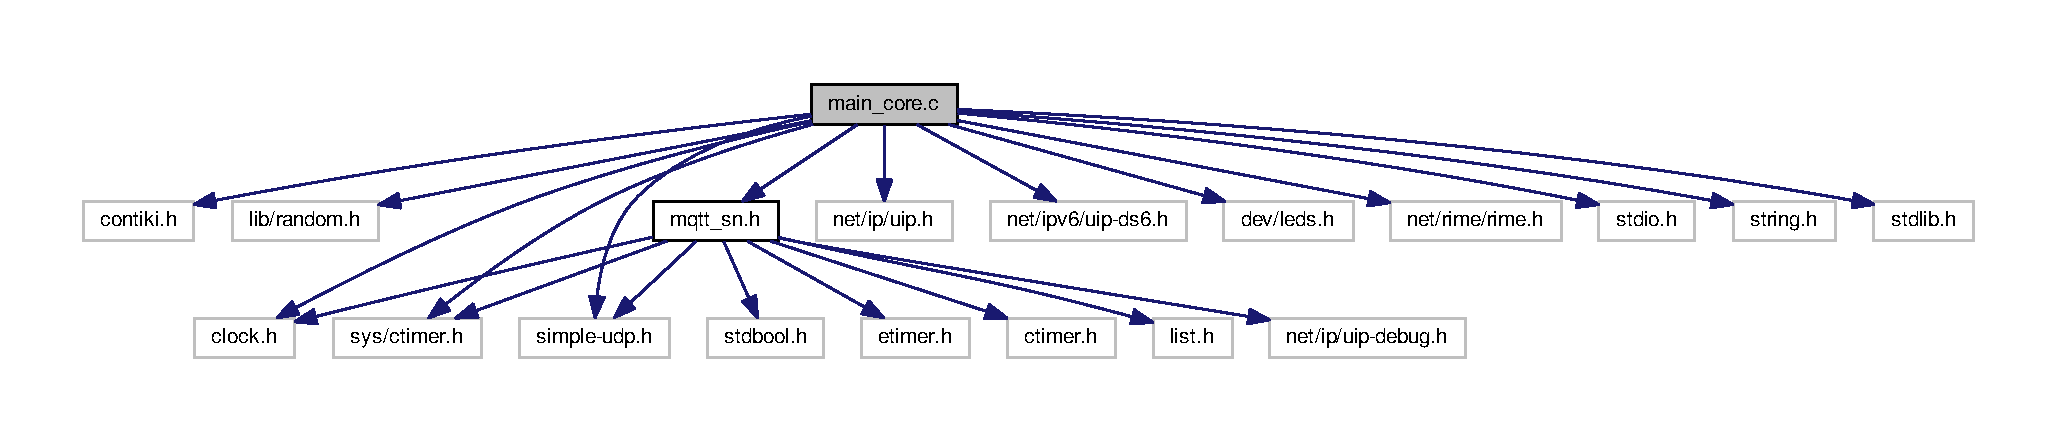
\includegraphics[width=350pt]{main__core_8c__incl}
\end{center}
\end{figure}
\subsection*{Funções}
\begin{DoxyCompactItemize}
\item 
\hypertarget{main__core_8c_a0a43995afea1479f111fbc2e35be0a7c}{void {\bfseries mqtt\+\_\+sn\+\_\+callback} (char $\ast$topic, char $\ast$message)}\label{main__core_8c_a0a43995afea1479f111fbc2e35be0a7c}

\item 
\hypertarget{main__core_8c_a271e0d9822452758a68f6e167c5209f8}{void {\bfseries init\+\_\+broker} (void)}\label{main__core_8c_a271e0d9822452758a68f6e167c5209f8}

\item 
\hypertarget{main__core_8c_a79354dfce54fd0bece29f8d443321b88}{{\bfseries P\+R\+O\+C\+E\+S\+S} (init\+\_\+system\+\_\+process,\char`\"{}\mbox{[}Contiki-\/O\+S\mbox{]} Iniciando sistema operacional\char`\"{})}\label{main__core_8c_a79354dfce54fd0bece29f8d443321b88}

\item 
\hypertarget{main__core_8c_a7683f5bdcb8cfbbb750ce92e76d1b7eb}{{\bfseries P\+R\+O\+C\+E\+S\+S\+\_\+\+T\+H\+R\+E\+A\+D} (init\+\_\+system\+\_\+process, ev, data)}\label{main__core_8c_a7683f5bdcb8cfbbb750ce92e76d1b7eb}

\end{DoxyCompactItemize}
\subsection*{Variáveis}
\begin{DoxyCompactItemize}
\item 
\hypertarget{main__core_8c_a5ca81254b9031056ba22742fb2252fd0}{\hyperlink{structmqtt__sn__con__t}{mqtt\+\_\+sn\+\_\+con\+\_\+t} {\bfseries mqtt\+\_\+sn\+\_\+connection}}\label{main__core_8c_a5ca81254b9031056ba22742fb2252fd0}

\item 
\hypertarget{main__core_8c_ac531a18312af7e29d65ccde0edd8b894}{A\+U\+T\+O\+S\+T\+A\+R\+T\+\_\+\+P\+R\+O\+C\+E\+S\+S\+E\+S \& {\bfseries init\+\_\+system\+\_\+process}}\label{main__core_8c_ac531a18312af7e29d65ccde0edd8b894}

\end{DoxyCompactItemize}


\subsection{Descrição detalhada}
Arquivo principal do porte do M\+Q\+T\+T-\/\+S\+N, utilizado para testar. 

\begin{DoxyAuthor}{Autor}
Ânderson Ignácio da Silva 
\end{DoxyAuthor}
\begin{DoxyDate}{Data}
19 Ago 2016 
\end{DoxyDate}
\begin{DoxySeeAlso}{Veja também}
\href{http://www.aignacio.com}{\tt http\+://www.\+aignacio.\+com} 
\end{DoxySeeAlso}

\hypertarget{mqtt__sn_8c}{\section{Referência ao ficheiro mqtt\+\_\+sn.\+c}
\label{mqtt__sn_8c}\index{mqtt\+\_\+sn.\+c@{mqtt\+\_\+sn.\+c}}
}


Arquivo principal do código fonte do porte do M\+Q\+T\+T-\/\+S\+N para o Contiki.  


{\ttfamily \#include \char`\"{}contiki.\+h\char`\"{}}\\*
{\ttfamily \#include \char`\"{}net/ip/uip.\+h\char`\"{}}\\*
{\ttfamily \#include \char`\"{}net/ipv6/uip-\/ds6.\+h\char`\"{}}\\*
{\ttfamily \#include \char`\"{}simple-\/udp.\+h\char`\"{}}\\*
{\ttfamily \#include $<$stdio.\+h$>$}\\*
{\ttfamily \#include $<$string.\+h$>$}\\*
{\ttfamily \#include $<$mqtt\+\_\+sn.\+h$>$}\\*
{\ttfamily \#include \char`\"{}sys/timer.\+h\char`\"{}}\\*
{\ttfamily \#include \char`\"{}list.\+h\char`\"{}}\\*
{\ttfamily \#include \char`\"{}sys/ctimer.\+h\char`\"{}}\\*
{\ttfamily \#include \char`\"{}sys/etimer.\+h\char`\"{}}\\*
{\ttfamily \#include \char`\"{}stdint.\+h\char`\"{}}\\*
{\ttfamily \#include $<$stdlib.\+h$>$}\\*
{\ttfamily \#include $<$stdbool.\+h$>$}\\*
Diagrama de dependências de inclusão para mqtt\+\_\+sn.\+c\+:
\nopagebreak
\begin{figure}[H]
\begin{center}
\leavevmode
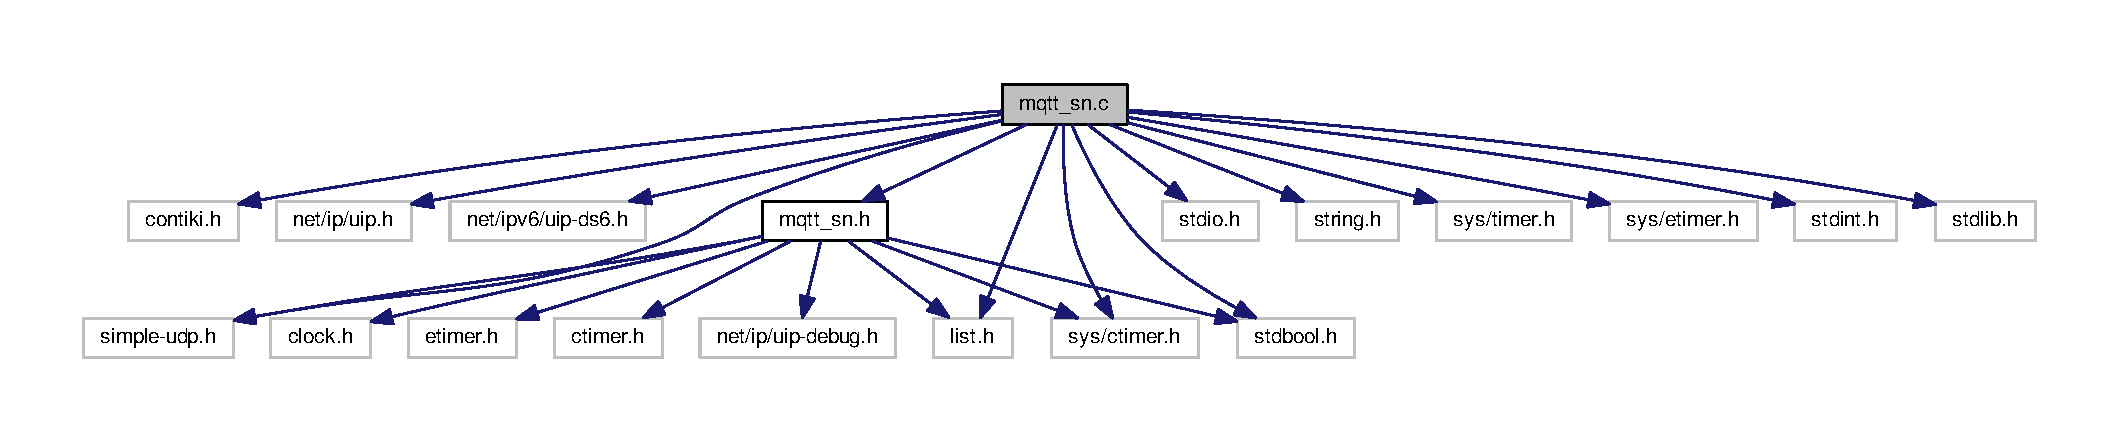
\includegraphics[width=350pt]{mqtt__sn_8c__incl}
\end{center}
\end{figure}
\subsection*{Funções}
\begin{DoxyCompactItemize}
\item 
\hypertarget{mqtt__sn_8c_a3d0423866ea0d39d4356fb107fcd256b}{{\bfseries P\+R\+O\+C\+E\+S\+S} (mqtt\+\_\+sn\+\_\+main,\char`\"{}\mbox{[}M\+Q\+T\+T-\/S\+N\mbox{]} Processo inicial\char`\"{})}\label{mqtt__sn_8c_a3d0423866ea0d39d4356fb107fcd256b}

\item 
bool \hyperlink{mqtt__sn_8c_a2620f37584b501fde35e71806a78b35a}{unlock\+\_\+tasks} (void)
\begin{DoxyCompactList}\small\item\em Libera opção de geração de tarefas. \end{DoxyCompactList}\item 
void \hyperlink{mqtt__sn_8c_ae0cb1cb4ad61ca752d66b286f839d72b}{init\+\_\+sub} (void $\ast$ptr)
\begin{DoxyCompactList}\small\item\em Inicia o evento de S\+U\+B\+S\+C\+R\+I\+B\+E. \end{DoxyCompactList}\item 
void \hyperlink{mqtt__sn_8c_ac598f98e844bfd5bbdb577099ddf06d1}{parse\+\_\+mqtt\+\_\+type\+\_\+string} (uint8\+\_\+t type, char $\ast$$\ast$type\+\_\+string)
\begin{DoxyCompactList}\small\item\em Retorna a string de status correspondente. \end{DoxyCompactList}\item 
char $\ast$ \hyperlink{mqtt__sn_8c_a9bd6d4e9304d00d28861751c22b146e4}{mqtt\+\_\+sn\+\_\+check\+\_\+status\+\_\+string} (void)
\begin{DoxyCompactList}\small\item\em Checa o status da conexãoe em String. \end{DoxyCompactList}\item 
\hyperlink{mqtt__sn_8h_aab2bca192b63f37bf4847be3686bca75}{mqtt\+\_\+sn\+\_\+status\+\_\+t} \hyperlink{mqtt__sn_8c_a200e89a8fd400c652431bd505de6f827}{mqtt\+\_\+sn\+\_\+check\+\_\+status} (void)
\begin{DoxyCompactList}\small\item\em Checa o status da conexão M\+Q\+T\+T-\/\+S\+N. \end{DoxyCompactList}\item 
\hyperlink{mqtt__sn_8h_add91ba4199db8665b9b9fc56fc6783a6}{resp\+\_\+con\+\_\+t} \hyperlink{mqtt__sn_8c_a172afa34fe10ad1ee4ffc0d226b35b4d}{mqtt\+\_\+sn\+\_\+check\+\_\+rc} (uint8\+\_\+t rc)
\begin{DoxyCompactList}\small\item\em Envia requisição de conexão ao broker M\+Q\+T\+T-\/\+S\+N. \end{DoxyCompactList}\item 
uint8\+\_\+t \hyperlink{mqtt__sn_8c_adba0283cc8fadf24f2f04246c76e8cde}{mqtt\+\_\+sn\+\_\+get\+\_\+qos\+\_\+flag} (int8\+\_\+t qos)
\begin{DoxyCompactList}\small\item\em Gera a flag de nível Qo\+S. \end{DoxyCompactList}\item 
\hyperlink{mqtt__sn_8h_add91ba4199db8665b9b9fc56fc6783a6}{resp\+\_\+con\+\_\+t} \hyperlink{mqtt__sn_8c_ac5fde757ae886c8827b853125f7458bd}{mqtt\+\_\+sn\+\_\+sub\+\_\+wildcard} (char $\ast$topic, uint8\+\_\+t qos)
\begin{DoxyCompactList}\small\item\em Prepara tarefa de S\+U\+B\+S\+C\+R\+I\+B\+E do tipo W\+I\+L\+D\+C\+A\+R\+D. \end{DoxyCompactList}\item 
\hyperlink{mqtt__sn_8h_add91ba4199db8665b9b9fc56fc6783a6}{resp\+\_\+con\+\_\+t} \hyperlink{mqtt__sn_8c_aab8d5db0224c9b083af9f18094053795}{mqtt\+\_\+sn\+\_\+sub} (char $\ast$topic, uint8\+\_\+t qos)
\begin{DoxyCompactList}\small\item\em Prepara requisição de inscrição ao broker M\+Q\+T\+T-\/\+S\+N. \end{DoxyCompactList}\item 
\hyperlink{mqtt__sn_8h_add91ba4199db8665b9b9fc56fc6783a6}{resp\+\_\+con\+\_\+t} \hyperlink{mqtt__sn_8c_ab8c0f238b41b373afb8b21e0f594b79d}{mqtt\+\_\+sn\+\_\+pub} (char $\ast$topic, char $\ast$message, bool retain\+\_\+flag, uint8\+\_\+t qos)
\begin{DoxyCompactList}\small\item\em Prepara requisição de publicação ao broker M\+Q\+T\+T-\/\+S\+N. \end{DoxyCompactList}\item 
\hyperlink{mqtt__sn_8h_add91ba4199db8665b9b9fc56fc6783a6}{resp\+\_\+con\+\_\+t} \hyperlink{mqtt__sn_8c_af60c0aa848adffbfe41a2e655a279f9d}{verf\+\_\+hist\+\_\+sub} (char $\ast$topic)
\begin{DoxyCompactList}\small\item\em Verifica se o tópico já foi registrado. \end{DoxyCompactList}\item 
\hyperlink{mqtt__sn_8h_add91ba4199db8665b9b9fc56fc6783a6}{resp\+\_\+con\+\_\+t} \hyperlink{mqtt__sn_8c_ac81a0d1e0daa51cdb8495a52e317e140}{verf\+\_\+register} (char $\ast$topic)
\begin{DoxyCompactList}\small\item\em Verifica pré-\/registro do tópico. \end{DoxyCompactList}\item 
void \hyperlink{mqtt__sn_8c_a6674e1ecf45890d3a15ab667fe4a4f58}{print\+\_\+g\+\_\+topics} (void)
\begin{DoxyCompactList}\small\item\em Exibe os tópicos registrados. \end{DoxyCompactList}\item 
void \hyperlink{mqtt__sn_8c_ada3c457ee81d0b29892742401845d918}{init\+\_\+vectors} (void)
\begin{DoxyCompactList}\small\item\em Inicializa os vetores M\+Q\+T\+T-\/\+S\+N. \end{DoxyCompactList}\item 
\hyperlink{mqtt__sn_8h_add91ba4199db8665b9b9fc56fc6783a6}{resp\+\_\+con\+\_\+t} \hyperlink{mqtt__sn_8c_adfb1174ee7cff21df2d0afbb6fe2db30}{mqtt\+\_\+sn\+\_\+will\+\_\+topic\+\_\+send} (void)
\begin{DoxyCompactList}\small\item\em Envia tópico de L\+W\+T. \end{DoxyCompactList}\item 
\hyperlink{mqtt__sn_8h_add91ba4199db8665b9b9fc56fc6783a6}{resp\+\_\+con\+\_\+t} \hyperlink{mqtt__sn_8c_a6718f310e6635c018a7126c5b1311e50}{mqtt\+\_\+sn\+\_\+will\+\_\+message\+\_\+send} (void)
\begin{DoxyCompactList}\small\item\em Envia mensagem de L\+W\+T. \end{DoxyCompactList}\item 
void \hyperlink{mqtt__sn_8c_af09083ea59a182fdf109b6e3fa213bec}{mqtt\+\_\+sn\+\_\+ping\+\_\+send} (void)
\begin{DoxyCompactList}\small\item\em Envia requisição de ping ao broker. \end{DoxyCompactList}\item 
\hyperlink{mqtt__sn_8h_add91ba4199db8665b9b9fc56fc6783a6}{resp\+\_\+con\+\_\+t} \hyperlink{mqtt__sn_8c_a1b8eb51076a2923f2c036f1ff925c168}{mqtt\+\_\+sn\+\_\+con\+\_\+send} (void)
\begin{DoxyCompactList}\small\item\em Envia requisição de conexão ao broker M\+Q\+T\+T-\/\+S\+N. \end{DoxyCompactList}\item 
\hyperlink{mqtt__sn_8h_add91ba4199db8665b9b9fc56fc6783a6}{resp\+\_\+con\+\_\+t} \hyperlink{mqtt__sn_8c_ae17664af7f894e29743fafdf8bf98f89}{mqtt\+\_\+sn\+\_\+reg\+\_\+send} (void)
\begin{DoxyCompactList}\small\item\em Envio de mensagens ao broker do tipo R\+E\+G\+I\+S\+T\+E\+R. \end{DoxyCompactList}\item 
\hyperlink{mqtt__sn_8h_add91ba4199db8665b9b9fc56fc6783a6}{resp\+\_\+con\+\_\+t} \hyperlink{mqtt__sn_8c_aa6e0e9b8d7769407ab35fec5443e3896}{mqtt\+\_\+sn\+\_\+regack\+\_\+send} (uint16\+\_\+t msg\+\_\+id, uint16\+\_\+t topic\+\_\+id)
\begin{DoxyCompactList}\small\item\em Envia pacote do tipo R\+E\+G\+A\+C\+K ao broker. \end{DoxyCompactList}\item 
\hyperlink{mqtt__sn_8h_add91ba4199db8665b9b9fc56fc6783a6}{resp\+\_\+con\+\_\+t} \hyperlink{mqtt__sn_8c_a550856b818c23fce9e4d5b253c3e7547}{mqtt\+\_\+sn\+\_\+pub\+\_\+send} (char $\ast$topic, char $\ast$message, bool retain\+\_\+flag, uint8\+\_\+t qos)
\begin{DoxyCompactList}\small\item\em Envia pacote P\+U\+B\+L\+I\+S\+H ao broker M\+Q\+T\+T-\/\+S\+N. \end{DoxyCompactList}\item 
\hyperlink{mqtt__sn_8h_add91ba4199db8665b9b9fc56fc6783a6}{resp\+\_\+con\+\_\+t} \hyperlink{mqtt__sn_8c_a105b8d440266b4a582f2d627e57be14a}{mqtt\+\_\+sn\+\_\+sub\+\_\+send} (char $\ast$topic, uint8\+\_\+t qos)
\begin{DoxyCompactList}\small\item\em Envia pacote S\+U\+B\+S\+C\+R\+I\+B\+E ao broker M\+Q\+T\+T-\/\+S\+N. \end{DoxyCompactList}\item 
\hyperlink{mqtt__sn_8h_add91ba4199db8665b9b9fc56fc6783a6}{resp\+\_\+con\+\_\+t} \hyperlink{mqtt__sn_8c_a831d03a2cd7fbc884cec2013c2ebc823}{mqtt\+\_\+sn\+\_\+sub\+\_\+send\+\_\+wildcard} (char $\ast$topic, uint8\+\_\+t qos)
\begin{DoxyCompactList}\small\item\em Envia pacote S\+U\+B\+S\+C\+R\+I\+B\+E do tipo W\+I\+L\+D\+C\+A\+R\+D ao broker M\+Q\+T\+T-\/\+S\+N. \end{DoxyCompactList}\item 
\hypertarget{mqtt__sn_8c_ade91c29dc851d7eef5fe46a9804b4d5e}{\hyperlink{mqtt__sn_8h_add91ba4199db8665b9b9fc56fc6783a6}{resp\+\_\+con\+\_\+t} {\bfseries mqtt\+\_\+sn\+\_\+disconnect} (uint16\+\_\+t duration)}\label{mqtt__sn_8c_ade91c29dc851d7eef5fe46a9804b4d5e}

\item 
\hyperlink{mqtt__sn_8h_add91ba4199db8665b9b9fc56fc6783a6}{resp\+\_\+con\+\_\+t} \hyperlink{mqtt__sn_8c_a575514d0f0fd3b6c5c4a2c75e604bf79}{mqtt\+\_\+sn\+\_\+insert\+\_\+queue} (\hyperlink{structmqtt__sn__task__t}{mqtt\+\_\+sn\+\_\+task\+\_\+t} new)
\begin{DoxyCompactList}\small\item\em Insere uma tarefa na fila. \end{DoxyCompactList}\item 
void \hyperlink{mqtt__sn_8c_aa17781596362470e100d5fc4f62a01e9}{mqtt\+\_\+sn\+\_\+delete\+\_\+queue} (void)
\begin{DoxyCompactList}\small\item\em Remove o elemento mais próximo de ser processado. \end{DoxyCompactList}\item 
void \hyperlink{mqtt__sn_8c_ae4f357f3a8fa7a65fa95b695288c5173}{mqtt\+\_\+sn\+\_\+check\+\_\+queue} (void)
\begin{DoxyCompactList}\small\item\em Lista as tarefas da fila. \end{DoxyCompactList}\item 
bool \hyperlink{mqtt__sn_8c_afb698c97e10afa31e2c11351f6ce9388}{mqtt\+\_\+sn\+\_\+check\+\_\+empty} (void)
\begin{DoxyCompactList}\small\item\em Checa o status da fila de tarefas M\+Q\+T\+T-\/\+S\+N. \end{DoxyCompactList}\item 
void \hyperlink{mqtt__sn_8c_af9146fa082fe2bc6612fb13dbb20ed36}{mqtt\+\_\+sn\+\_\+recv\+\_\+parser} (const uint8\+\_\+t $\ast$data)
\begin{DoxyCompactList}\small\item\em Realiza o parsing das mensagens U\+D\+P recebidas. \end{DoxyCompactList}\item 
void \hyperlink{mqtt__sn_8c_ab6fc2a07c15881877943348bef786cd8}{mqtt\+\_\+sn\+\_\+udp\+\_\+rec\+\_\+cb} (struct simple\+\_\+udp\+\_\+connection $\ast$c, const uip\+\_\+ipaddr\+\_\+t $\ast$sender\+\_\+addr, uint16\+\_\+t sender\+\_\+port, const uip\+\_\+ipaddr\+\_\+t $\ast$receiver\+\_\+addr, uint16\+\_\+t receiver\+\_\+port, const uint8\+\_\+t $\ast$data, uint16\+\_\+t datalen)
\begin{DoxyCompactList}\small\item\em Callback de recepção U\+D\+P. \end{DoxyCompactList}\item 
\hyperlink{mqtt__sn_8h_add91ba4199db8665b9b9fc56fc6783a6}{resp\+\_\+con\+\_\+t} \hyperlink{mqtt__sn_8c_a8771e78d9d8d5379ff27fba1feefe37c}{mqtt\+\_\+sn\+\_\+create\+\_\+sck} (\hyperlink{structmqtt__sn__con__t}{mqtt\+\_\+sn\+\_\+con\+\_\+t} mqtt\+\_\+sn\+\_\+connection, char $\ast$topics\mbox{[}$\,$\mbox{]}, size\+\_\+t topic\+\_\+len, \hyperlink{mqtt__sn_8h_a679e4bebc7798d960960760150bdc5a7}{mqtt\+\_\+sn\+\_\+cb\+\_\+f} cb\+\_\+f)
\begin{DoxyCompactList}\small\item\em Inicia conexão ao broker U\+D\+P. \end{DoxyCompactList}\item 
void \hyperlink{mqtt__sn_8c_a46fe607d1db728d41ed6aec6fee3fc77}{mqtt\+\_\+sn\+\_\+init} (void)
\begin{DoxyCompactList}\small\item\em Inicializa P\+R\+O\+C\+E\+S\+S\+\_\+\+T\+H\+R\+E\+A\+D M\+Q\+T\+T-\/\+S\+N. \end{DoxyCompactList}\item 
void \hyperlink{mqtt__sn_8c_ac9614aca44158215c43b8810e052939d}{timeout\+\_\+con} (void $\ast$ptr)
\begin{DoxyCompactList}\small\item\em Processa timeout de pacotes. \end{DoxyCompactList}\item 
void \hyperlink{mqtt__sn_8c_a35dbd49b5fdc1d6e3dfe2b2d7255cf3e}{timeout\+\_\+ping\+\_\+mqtt} (void $\ast$ptr)
\begin{DoxyCompactList}\small\item\em Processa timeout de ping. \end{DoxyCompactList}\item 
\hypertarget{mqtt__sn_8c_ac4ada750a373f3b01262465d9b3dd468}{{\bfseries P\+R\+O\+C\+E\+S\+S\+\_\+\+T\+H\+R\+E\+A\+D} (mqtt\+\_\+sn\+\_\+main, ev, data)}\label{mqtt__sn_8c_ac4ada750a373f3b01262465d9b3dd468}

\end{DoxyCompactItemize}


\subsection{Descrição detalhada}
Arquivo principal do código fonte do porte do M\+Q\+T\+T-\/\+S\+N para o Contiki. 

\begin{DoxyAuthor}{Autor}
Ânderson Ignácio da Silva 
\end{DoxyAuthor}
\begin{DoxyDate}{Data}
19 Ago 2016 
\end{DoxyDate}
\begin{DoxySeeAlso}{Veja também}
\href{http://www.aignacio.com}{\tt http\+://www.\+aignacio.\+com} @ \mbox{[}Apontamento n-\/1\mbox{]}\+: Descoberta uma característica do contiki, o que ocorre é que se você utiliza algum temporizador de evento (etimer) e ele expira, ele gera um evento o que e esperado, porém se você tiver testando diversas condições de forma sequencial 1) else if(ev == etimer\+\_\+expired(....)) 2) else if(ev == mqtt\+\_\+event\+\_\+regack) ... M\+E\+S\+M\+O após ter gerado o evento de \char`\"{}expiração\char`\"{}, caso a condição 1) esteja antes da 2), e a 2) que gerou um evento, a 1) será executada anteriormente porque compreendesse que o \char`\"{}timer continua expirado\char`\"{}.
\end{DoxySeeAlso}
\mbox{[}Apontamento n-\/2\mbox{]}\+: Como nesta A\+P\+I utiliza-\/se malloc necessitamos da função do tipo P\+O\+S\+I\+X chamadas \char`\"{}sbrk\char`\"{} a qual utiliza de chamadas de sistema para realizar a operação de aloca ção de memória.\+Logo, devemos incluir no arquivo principal o arquivo \hyperlink{syscalls_8c}{syscalls.\+c} (arquivo disponibilizado pelo contiki -\/ lib/newlib/syscalls.\+c) e também deve-\/ mos incluir as variáveis \+\_\+heap e \+\_\+eheap no linker script (cc26xx.\+ld) para a função sbrk saber onde começa e termina a zona heap de memória do mcu.

Incluir no linker\+: ... \+\_\+heap = .; \+\_\+eheap = O\+R\+I\+G\+I\+N(\+S\+R\+A\+M) + L\+E\+N\+G\+T\+H(\+S\+R\+A\+M); \} 

\subsection{Documentação das funções}
\hypertarget{mqtt__sn_8c_ae0cb1cb4ad61ca752d66b286f839d72b}{\index{mqtt\+\_\+sn.\+c@{mqtt\+\_\+sn.\+c}!init\+\_\+sub@{init\+\_\+sub}}
\index{init\+\_\+sub@{init\+\_\+sub}!mqtt\+\_\+sn.\+c@{mqtt\+\_\+sn.\+c}}
\subsubsection[{init\+\_\+sub}]{\setlength{\rightskip}{0pt plus 5cm}void init\+\_\+sub (
\begin{DoxyParamCaption}
\item[{void $\ast$}]{ptr}
\end{DoxyParamCaption}
)}}\label{mqtt__sn_8c_ae0cb1cb4ad61ca752d66b286f839d72b}


Inicia o evento de S\+U\+B\+S\+C\+R\+I\+B\+E. 

Inicia as requisições de inscrição através do evento


\begin{DoxyParams}[1]{Parâmetros}
\mbox{\tt in}  & {\em 0} & Não recebe argumento\\
\hline
\end{DoxyParams}

\begin{DoxyRetVals}{Valores retornados}
{\em 0} & Não retorna argumento \\
\hline
\end{DoxyRetVals}

\begin{DoxyCode}
98                         \{
99   debug\_mqtt(\textcolor{stringliteral}{"INICIANDO SUBSCRIBE"});
100   process\_post(&mqtt\_sn\_main,mqtt\_event\_run\_task,NULL);
101 \}
\end{DoxyCode}
\hypertarget{mqtt__sn_8c_ada3c457ee81d0b29892742401845d918}{\index{mqtt\+\_\+sn.\+c@{mqtt\+\_\+sn.\+c}!init\+\_\+vectors@{init\+\_\+vectors}}
\index{init\+\_\+vectors@{init\+\_\+vectors}!mqtt\+\_\+sn.\+c@{mqtt\+\_\+sn.\+c}}
\subsubsection[{init\+\_\+vectors}]{\setlength{\rightskip}{0pt plus 5cm}void init\+\_\+vectors (
\begin{DoxyParamCaption}
\item[{void}]{}
\end{DoxyParamCaption}
)}}\label{mqtt__sn_8c_ada3c457ee81d0b29892742401845d918}


Inicializa os vetores M\+Q\+T\+T-\/\+S\+N. 

Deleta tarefas na fila e inicializa o vetor de tópicos setando 0x\+F\+F aos identificadores de tópico


\begin{DoxyParams}[1]{Parâmetros}
\mbox{\tt in}  & {\em 0} & Não recebe argumento\\
\hline
\end{DoxyParams}

\begin{DoxyRetVals}{Valores retornados}
{\em 0} & Não retorna argumento \\
\hline
\end{DoxyRetVals}

\begin{DoxyCode}
331                        \{
332   debug\_mqtt(\textcolor{stringliteral}{"Inicializando vetores..."});
333   \textcolor{keywordtype}{size\_t} i;
334   \textcolor{keywordflow}{for} (i = 1; i < \hyperlink{group__MQTT__SN__CONTROL_ga5ed98e8fc00194886ebc14d25540f81b}{MAX\_TOPIC\_USED}; i++)\{
335     g\_topic\_bind[i].short\_topic\_id = 0xFF;
336     g\_topic\_bind[i].topic\_name = 0;
337     g\_topic\_bind[i].subscribed = 0x00;
338   \}
339 
340   \textcolor{keywordflow}{while} (!\hyperlink{mqtt__sn_8c_afb698c97e10afa31e2c11351f6ce9388}{mqtt\_sn\_check\_empty}())
341       \hyperlink{mqtt__sn_8c_aa17781596362470e100d5fc4f62a01e9}{mqtt\_sn\_delete\_queue}();
342   g\_task\_id = 0;
343 \}
\end{DoxyCode}
\hypertarget{mqtt__sn_8c_afb698c97e10afa31e2c11351f6ce9388}{\index{mqtt\+\_\+sn.\+c@{mqtt\+\_\+sn.\+c}!mqtt\+\_\+sn\+\_\+check\+\_\+empty@{mqtt\+\_\+sn\+\_\+check\+\_\+empty}}
\index{mqtt\+\_\+sn\+\_\+check\+\_\+empty@{mqtt\+\_\+sn\+\_\+check\+\_\+empty}!mqtt\+\_\+sn.\+c@{mqtt\+\_\+sn.\+c}}
\subsubsection[{mqtt\+\_\+sn\+\_\+check\+\_\+empty}]{\setlength{\rightskip}{0pt plus 5cm}bool mqtt\+\_\+sn\+\_\+check\+\_\+empty (
\begin{DoxyParamCaption}
\item[{void}]{}
\end{DoxyParamCaption}
)}}\label{mqtt__sn_8c_afb698c97e10afa31e2c11351f6ce9388}


Checa o status da fila de tarefas M\+Q\+T\+T-\/\+S\+N. 

Percorra a lista encadeada de tarefas para verificar se está vazia


\begin{DoxyParams}[1]{Parâmetros}
\mbox{\tt in}  & {\em 0} & Não recebe argumento\\
\hline
\end{DoxyParams}

\begin{DoxyRetVals}{Valores retornados}
{\em T\+R\+U\+E} & Fila vazia \\
\hline
{\em F\+A\+L\+S\+E} & Há tarefas a serem processadas \\
\hline
\end{DoxyRetVals}

\begin{DoxyCode}
691                               \{
692   \textcolor{keywordflow}{if} (mqtt\_queue\_first  ==  NULL)
693     \textcolor{keywordflow}{return} \textcolor{keyword}{true};
694   \textcolor{keywordflow}{else}
695     \textcolor{keywordflow}{return} \textcolor{keyword}{false};
696 \}
\end{DoxyCode}
\hypertarget{mqtt__sn_8c_ae4f357f3a8fa7a65fa95b695288c5173}{\index{mqtt\+\_\+sn.\+c@{mqtt\+\_\+sn.\+c}!mqtt\+\_\+sn\+\_\+check\+\_\+queue@{mqtt\+\_\+sn\+\_\+check\+\_\+queue}}
\index{mqtt\+\_\+sn\+\_\+check\+\_\+queue@{mqtt\+\_\+sn\+\_\+check\+\_\+queue}!mqtt\+\_\+sn.\+c@{mqtt\+\_\+sn.\+c}}
\subsubsection[{mqtt\+\_\+sn\+\_\+check\+\_\+queue}]{\setlength{\rightskip}{0pt plus 5cm}void mqtt\+\_\+sn\+\_\+check\+\_\+queue (
\begin{DoxyParamCaption}
{}
\end{DoxyParamCaption}
)}}\label{mqtt__sn_8c_ae4f357f3a8fa7a65fa95b695288c5173}


Lista as tarefas da fila. 

Percorre os links dos ponteiros listando os elementos a serem processados pela A\+S\+M do M\+Q\+T\+T-\/\+S\+N


\begin{DoxyParams}[1]{Parâmetros}
\mbox{\tt in}  & {\em 0} & Não recebe argumento\\
\hline
\end{DoxyParams}

\begin{DoxyRetVals}{Valores retornados}
{\em 0} & Não retorna nada \\
\hline
\end{DoxyRetVals}

\begin{DoxyCode}
672                               \{
673   \textcolor{keywordtype}{int} cnt = 0;
674   \textcolor{keyword}{struct }\hyperlink{structnode}{node} *temp;
675   \textcolor{keywordtype}{char} *task\_type;
676 
677   temp = mqtt\_queue\_first;
678 
679   debug\_task(\textcolor{stringliteral}{"VALOR DO GLOBAL ID g\_task\_id:%d"},g\_task\_id);
680 
681   debug\_task(\textcolor{stringliteral}{"FILA:"});
682   \textcolor{keywordflow}{while} (temp) \{
683       \hyperlink{mqtt__sn_8c_ac598f98e844bfd5bbdb577099ddf06d1}{parse\_mqtt\_type\_string}(temp->data.\hyperlink{structmqtt__sn__task__t_afb14d280d486f10af744fb1ac7f145eb}{msg\_type\_q},&task\_type);
684       debug\_task(\textcolor{stringliteral}{"[%2.0d][%s][%d]"},(\textcolor{keywordtype}{int})temp->data.\hyperlink{structmqtt__sn__task__t_a1dba79ab8685a56d3ae57d84aca21ce8}{id\_task}, task\_type,temp->data.
      \hyperlink{structmqtt__sn__task__t_a25bc8ea535927589bca3720e0e838958}{short\_topic});
685       temp = temp->link;
686       cnt++;
687   \}
688   debug\_task(\textcolor{stringliteral}{"Tamanho da fila:[%d]"}, cnt);
689 \}
\end{DoxyCode}
\hypertarget{mqtt__sn_8c_a172afa34fe10ad1ee4ffc0d226b35b4d}{\index{mqtt\+\_\+sn.\+c@{mqtt\+\_\+sn.\+c}!mqtt\+\_\+sn\+\_\+check\+\_\+rc@{mqtt\+\_\+sn\+\_\+check\+\_\+rc}}
\index{mqtt\+\_\+sn\+\_\+check\+\_\+rc@{mqtt\+\_\+sn\+\_\+check\+\_\+rc}!mqtt\+\_\+sn.\+c@{mqtt\+\_\+sn.\+c}}
\subsubsection[{mqtt\+\_\+sn\+\_\+check\+\_\+rc}]{\setlength{\rightskip}{0pt plus 5cm}{\bf resp\+\_\+con\+\_\+t} mqtt\+\_\+sn\+\_\+check\+\_\+rc (
\begin{DoxyParamCaption}
\item[{uint8\+\_\+t}]{rc}
\end{DoxyParamCaption}
)}}\label{mqtt__sn_8c_a172afa34fe10ad1ee4ffc0d226b35b4d}


Envia requisição de conexão ao broker M\+Q\+T\+T-\/\+S\+N. 

Realiza o envio de mensagens do tipo C\+O\+N\+N\+E\+C\+T ao broker M\+Q\+T\+T-\/\+S\+N


\begin{DoxyParams}[1]{Parâmetros}
\mbox{\tt in}  & {\em rc} & Código de retorno da requisição M\+Q\+T\+T (Return Code)\\
\hline
\end{DoxyParams}

\begin{DoxyRetVals}{Valores retornados}
{\em F\+A\+I\+L\+\_\+\+C\+O\+N} & Falha por algum motivo no código de retorno \\
\hline
{\em S\+U\+C\+C\+E\+S\+S\+\_\+\+C\+O\+N} & Sucesso no recebimento do código de retorno\\
\hline
\end{DoxyRetVals}
\begin{DoxyRefDesc}{Tarefa}
\item[\hyperlink{todo__todo000006}{Tarefa}]Expandir o tipo de falha para tornar mais precisa a depuração futura \end{DoxyRefDesc}

\begin{DoxyCode}
174                                        \{
175   \textcolor{keywordflow}{switch} (rc) \{
176     \textcolor{keywordflow}{case} ACCEPTED:
177       \textcolor{keywordflow}{return} \hyperlink{mqtt__sn_8h_a754c1055b4431040415cf01b39caaa98ae7b7a388c90c2c5428cced225760885f}{SUCCESS\_CON};
178     \textcolor{keywordflow}{break};
179     \textcolor{keywordflow}{case} REJECTED\_CONGESTION:
180       \textcolor{keywordflow}{return} \hyperlink{mqtt__sn_8h_a754c1055b4431040415cf01b39caaa98ac6ae922662cbaf7958eb387bfd6fe4da}{FAIL\_CON};
181     \textcolor{keywordflow}{break};
182     \textcolor{keywordflow}{case} REJECTED\_INVALID\_TOPIC\_ID:
183       \textcolor{keywordflow}{return} \hyperlink{mqtt__sn_8h_a754c1055b4431040415cf01b39caaa98ac6ae922662cbaf7958eb387bfd6fe4da}{FAIL\_CON};
184     \textcolor{keywordflow}{break};
185     \textcolor{keywordflow}{case} REJECTED\_NOT\_SUPPORTED:
186       \textcolor{keywordflow}{return} \hyperlink{mqtt__sn_8h_a754c1055b4431040415cf01b39caaa98ac6ae922662cbaf7958eb387bfd6fe4da}{FAIL\_CON};
187     \textcolor{keywordflow}{break};
188     \textcolor{keywordflow}{default}:
189       \textcolor{keywordflow}{return} \hyperlink{mqtt__sn_8h_a754c1055b4431040415cf01b39caaa98ac6ae922662cbaf7958eb387bfd6fe4da}{FAIL\_CON};
190     \textcolor{keywordflow}{break};
191   \}
192 \}
\end{DoxyCode}
\hypertarget{mqtt__sn_8c_a200e89a8fd400c652431bd505de6f827}{\index{mqtt\+\_\+sn.\+c@{mqtt\+\_\+sn.\+c}!mqtt\+\_\+sn\+\_\+check\+\_\+status@{mqtt\+\_\+sn\+\_\+check\+\_\+status}}
\index{mqtt\+\_\+sn\+\_\+check\+\_\+status@{mqtt\+\_\+sn\+\_\+check\+\_\+status}!mqtt\+\_\+sn.\+c@{mqtt\+\_\+sn.\+c}}
\subsubsection[{mqtt\+\_\+sn\+\_\+check\+\_\+status}]{\setlength{\rightskip}{0pt plus 5cm}{\bf mqtt\+\_\+sn\+\_\+status\+\_\+t} mqtt\+\_\+sn\+\_\+check\+\_\+status (
\begin{DoxyParamCaption}
\item[{void}]{}
\end{DoxyParamCaption}
)}}\label{mqtt__sn_8c_a200e89a8fd400c652431bd505de6f827}


Checa o status da conexão M\+Q\+T\+T-\/\+S\+N. 

Retorna o status da conexão M\+Q\+T\+T-\/\+S\+N baseado na estrutura mqtt\+\_\+sn\+\_\+status\+\_\+t


\begin{DoxyParams}[1]{Parâmetros}
\mbox{\tt in}  & {\em 0} & Não recebe argumento\\
\hline
\end{DoxyParams}

\begin{DoxyRetVals}{Valores retornados}
{\em mqtt\+\_\+sn\+\_\+status\+\_\+t} & Estado da conexão \\
\hline
\end{DoxyRetVals}

\begin{DoxyCode}
170                                            \{
171   \textcolor{keywordflow}{return} mqtt\_status;
172 \}
\end{DoxyCode}
\hypertarget{mqtt__sn_8c_a9bd6d4e9304d00d28861751c22b146e4}{\index{mqtt\+\_\+sn.\+c@{mqtt\+\_\+sn.\+c}!mqtt\+\_\+sn\+\_\+check\+\_\+status\+\_\+string@{mqtt\+\_\+sn\+\_\+check\+\_\+status\+\_\+string}}
\index{mqtt\+\_\+sn\+\_\+check\+\_\+status\+\_\+string@{mqtt\+\_\+sn\+\_\+check\+\_\+status\+\_\+string}!mqtt\+\_\+sn.\+c@{mqtt\+\_\+sn.\+c}}
\subsubsection[{mqtt\+\_\+sn\+\_\+check\+\_\+status\+\_\+string}]{\setlength{\rightskip}{0pt plus 5cm}char$\ast$ mqtt\+\_\+sn\+\_\+check\+\_\+status\+\_\+string (
\begin{DoxyParamCaption}
\item[{void}]{}
\end{DoxyParamCaption}
)}}\label{mqtt__sn_8c_a9bd6d4e9304d00d28861751c22b146e4}


Checa o status da conexãoe em String. 

Verifica o status da conexão M\+Q\+T\+T-\/\+S\+N e retorna uma string com o estado


\begin{DoxyParams}[1]{Parâmetros}
\mbox{\tt in}  & {\em Não} & recebe argumento\\
\hline
\end{DoxyParams}

\begin{DoxyRetVals}{Valores retornados}
{\em S\+T\+R\+I\+N\+G} & String do estado atual da conexão M\+Q\+T\+T-\/\+S\+N \\
\hline
\end{DoxyRetVals}

\begin{DoxyCode}
141                                        \{
142   \textcolor{keywordflow}{switch} (mqtt\_status) \{
143     \textcolor{keywordflow}{case} MQTTSN\_DISCONNECTED:
144       \textcolor{keywordflow}{return} \textcolor{stringliteral}{"DESCONECTADO"};
145     \textcolor{keywordflow}{break};
146     \textcolor{keywordflow}{case} MQTTSN\_WAITING\_CONNACK:
147       \textcolor{keywordflow}{return} \textcolor{stringliteral}{"AGUARDANDO CONNACK"};
148     \textcolor{keywordflow}{break};
149     \textcolor{keywordflow}{case} MQTTSN\_WAITING\_REGACK:
150       \textcolor{keywordflow}{return} \textcolor{stringliteral}{"AGUARDANDO REGACK"};
151     \textcolor{keywordflow}{break};
152     \textcolor{keywordflow}{case} MQTTSN\_CONNECTED:
153       \textcolor{keywordflow}{return} \textcolor{stringliteral}{"#### CONECTADO ####"};
154     \textcolor{keywordflow}{break};
155     \textcolor{keywordflow}{case} MQTTSN\_TOPIC\_REGISTERED:
156       \textcolor{keywordflow}{return} \textcolor{stringliteral}{"TOPICOS REGISTRADOS"};
157     \textcolor{keywordflow}{break};
158     \textcolor{keywordflow}{case} MQTTSN\_WAITING\_WILLTOPICREQ:
159       \textcolor{keywordflow}{return} \textcolor{stringliteral}{"AGUARDANDO WILL TOPIC"};
160     \textcolor{keywordflow}{break};
161     \textcolor{keywordflow}{case} MQTTSN\_WAITING\_WILLMSGREQ:
162       \textcolor{keywordflow}{return} \textcolor{stringliteral}{"AGUARDANDO WILL MESSAGE"};
163     \textcolor{keywordflow}{break};
164     \textcolor{keywordflow}{default}:
165       \textcolor{keywordflow}{return} \textcolor{stringliteral}{"ESTADO NAO DESCRITO"};
166     \textcolor{keywordflow}{break};
167   \}
168 \}
\end{DoxyCode}
\hypertarget{mqtt__sn_8c_a1b8eb51076a2923f2c036f1ff925c168}{\index{mqtt\+\_\+sn.\+c@{mqtt\+\_\+sn.\+c}!mqtt\+\_\+sn\+\_\+con\+\_\+send@{mqtt\+\_\+sn\+\_\+con\+\_\+send}}
\index{mqtt\+\_\+sn\+\_\+con\+\_\+send@{mqtt\+\_\+sn\+\_\+con\+\_\+send}!mqtt\+\_\+sn.\+c@{mqtt\+\_\+sn.\+c}}
\subsubsection[{mqtt\+\_\+sn\+\_\+con\+\_\+send}]{\setlength{\rightskip}{0pt plus 5cm}{\bf resp\+\_\+con\+\_\+t} mqtt\+\_\+sn\+\_\+con\+\_\+send (
\begin{DoxyParamCaption}
\item[{void}]{}
\end{DoxyParamCaption}
)}}\label{mqtt__sn_8c_a1b8eb51076a2923f2c036f1ff925c168}


Envia requisição de conexão ao broker M\+Q\+T\+T-\/\+S\+N. 

Realiza o envio de mensagens do tipo C\+O\+N\+N\+E\+C\+T ao broker M\+Q\+T\+T-\/\+S\+N


\begin{DoxyParams}[1]{Parâmetros}
\mbox{\tt in}  & {\em 0} & Não recebe argumento\\
\hline
\end{DoxyParams}

\begin{DoxyRetVals}{Valores retornados}
{\em F\+A\+I\+L\+\_\+\+C\+O\+N} & Falha ao enviar o pacote C\+O\+N\+N\+E\+C\+T \\
\hline
{\em S\+U\+C\+C\+E\+S\+S\+\_\+\+C\+O\+N} & Sucesso ao enviar o pacote C\+O\+N\+N\+E\+C\+T \\
\hline
\end{DoxyRetVals}

\begin{DoxyCode}
404                                  \{
405   \hyperlink{structconnect__packet__t}{connect\_packet\_t} packet;
406 
407   \textcolor{comment}{// Criação do pacote CONNECT}
408   packet.type = MQTT\_SN\_TYPE\_CONNECT;
409   packet.flags = MQTT\_SN\_FLAG\_CLEAN;
410   \textcolor{keywordflow}{if} (g\_will)
411     packet.flags += MQTT\_SN\_FLAG\_WILL;
412   packet.protocol\_id = MQTT\_SN\_PROTOCOL\_ID;
413   packet.duration = uip\_htons(g\_mqtt\_sn\_con.\hyperlink{structmqtt__sn__con__t_a276b967ec5d6e3305ee4695488e4472b}{keep\_alive}); \textcolor{comment}{//Realiza a conversão para network byte
       order}
414 
415   strncpy(packet.client\_id, g\_mqtt\_sn\_con.\hyperlink{structmqtt__sn__con__t_a3880622ca383fee22fbbac18442bae32}{client\_id}, strlen(g\_mqtt\_sn\_con.
      \hyperlink{structmqtt__sn__con__t_a3880622ca383fee22fbbac18442bae32}{client\_id}));
416   packet.client\_id[strlen(g\_mqtt\_sn\_con.\hyperlink{structmqtt__sn__con__t_a3880622ca383fee22fbbac18442bae32}{client\_id})] = \textcolor{charliteral}{'\(\backslash\)0'};
417   packet.length = 0x06 + strlen(packet.client\_id);
418 
419   \textcolor{comment}{// debug\_mqtt("CLIENT\_ID:%s, Tamanho:%d",packet.client\_id,strlen(packet.client\_id));}
420   debug\_mqtt(\textcolor{stringliteral}{"Enviando o pacote @CONNECT "});
421   simple\_udp\_send(&g\_mqtt\_sn\_con.udp\_con,&packet, packet.length);
422   \textcolor{comment}{// debug\_mqtt("enviado!");}
423   \textcolor{keywordflow}{return} \hyperlink{mqtt__sn_8h_a754c1055b4431040415cf01b39caaa98ae7b7a388c90c2c5428cced225760885f}{SUCCESS\_CON};
424 \}
\end{DoxyCode}
\hypertarget{mqtt__sn_8c_a8771e78d9d8d5379ff27fba1feefe37c}{\index{mqtt\+\_\+sn.\+c@{mqtt\+\_\+sn.\+c}!mqtt\+\_\+sn\+\_\+create\+\_\+sck@{mqtt\+\_\+sn\+\_\+create\+\_\+sck}}
\index{mqtt\+\_\+sn\+\_\+create\+\_\+sck@{mqtt\+\_\+sn\+\_\+create\+\_\+sck}!mqtt\+\_\+sn.\+c@{mqtt\+\_\+sn.\+c}}
\subsubsection[{mqtt\+\_\+sn\+\_\+create\+\_\+sck}]{\setlength{\rightskip}{0pt plus 5cm}{\bf resp\+\_\+con\+\_\+t} mqtt\+\_\+sn\+\_\+create\+\_\+sck (
\begin{DoxyParamCaption}
\item[{{\bf mqtt\+\_\+sn\+\_\+con\+\_\+t}}]{mqtt\+\_\+sn\+\_\+connection, }
\item[{char $\ast$}]{topics\mbox{[}$\,$\mbox{]}, }
\item[{size\+\_\+t}]{topic\+\_\+len, }
\item[{{\bf mqtt\+\_\+sn\+\_\+cb\+\_\+f}}]{cb\+\_\+f}
\end{DoxyParamCaption}
)}}\label{mqtt__sn_8c_a8771e78d9d8d5379ff27fba1feefe37c}


Inicia conexão ao broker U\+D\+P. 

Estabelece a conexão com um servidor M\+Q\+T\+T-\/\+S\+N, através da porta 1884 além de iniciar a fila de processos de conexão do protocolo.


\begin{DoxyParams}[1]{Parâmetros}
\mbox{\tt in}  & {\em mqtt\+\_\+sn\+\_\+connection} & Estrutura padrão de comunicação M\+Q\+T\+T-\/\+S\+N \\
\hline
\mbox{\tt in}  & {\em topics} & Vetor de tópicos a serem registrados \\
\hline
\mbox{\tt in}  & {\em topic\+\_\+len} & Tamanho do vetor de tópicos a serem registrados \\
\hline
\mbox{\tt in}  & {\em mqtt\+\_\+sn\+\_\+cb\+\_\+f} & Ponteiro para função de callback para recebimento das mensagens M\+Q\+T\+T-\/\+S\+N\\
\hline
\end{DoxyParams}

\begin{DoxyRetVals}{Valores retornados}
{\em F\+A\+I\+L\+\_\+\+C\+O\+N} & Falha ao alocar conexão U\+D\+P \\
\hline
{\em S\+U\+C\+C\+E\+S\+S\+\_\+\+C\+O\+N} & Sucesso ao alocar conexão U\+D\+P \\
\hline
\end{DoxyRetVals}

\begin{DoxyCode}
858                                                                                                            
               \{
859   callback\_mqtt = cb\_f;
860   \textcolor{comment}{/************************************ RECONEXÃO******************************/}
861   topics\_len = topic\_len;
862   \textcolor{keywordtype}{size\_t} t = 0;
863   \textcolor{keywordflow}{for} (t=0; t < topic\_len; t++)\{
864     topics\_reconnect[t] = topics[t];
865     \textcolor{comment}{// debug\_mqtt("Armazenando topico: %s",(char *)topics\_reconnect[t]);}
866   \}
867   \textcolor{comment}{/************************************ RECONEXÃO******************************/}
868 
869   \textcolor{keyword}{static} uip\_ipaddr\_t broker\_addr;
870   \textcolor{keyword}{static} uint8\_t con\_udp\_status = 0;
871 
872   g\_mqtt\_sn\_con = mqtt\_sn\_connection;
873   uip\_ip6addr(&broker\_addr, *g\_mqtt\_sn\_con.\hyperlink{structmqtt__sn__con__t_a058796ada31936dced646e5da3eb329a}{ipv6\_broker},
874                             *(g\_mqtt\_sn\_con.\hyperlink{structmqtt__sn__con__t_a058796ada31936dced646e5da3eb329a}{ipv6\_broker}+1),
875                             *(g\_mqtt\_sn\_con.\hyperlink{structmqtt__sn__con__t_a058796ada31936dced646e5da3eb329a}{ipv6\_broker}+2),
876                             *(g\_mqtt\_sn\_con.\hyperlink{structmqtt__sn__con__t_a058796ada31936dced646e5da3eb329a}{ipv6\_broker}+3),
877                             *(g\_mqtt\_sn\_con.\hyperlink{structmqtt__sn__con__t_a058796ada31936dced646e5da3eb329a}{ipv6\_broker}+4),
878                             *(g\_mqtt\_sn\_con.\hyperlink{structmqtt__sn__con__t_a058796ada31936dced646e5da3eb329a}{ipv6\_broker}+5),
879                             *(g\_mqtt\_sn\_con.\hyperlink{structmqtt__sn__con__t_a058796ada31936dced646e5da3eb329a}{ipv6\_broker}+6),
880                             *(g\_mqtt\_sn\_con.\hyperlink{structmqtt__sn__con__t_a058796ada31936dced646e5da3eb329a}{ipv6\_broker}+7));
881 
882   \textcolor{keywordflow}{if} (strlen(g\_mqtt\_sn\_con.\hyperlink{structmqtt__sn__con__t_a3880622ca383fee22fbbac18442bae32}{client\_id}) > 23)\{
883     debug\_mqtt(\textcolor{stringliteral}{"Cli. ID SIZE:%d > 23!"},strlen(g\_mqtt\_sn\_con.\hyperlink{structmqtt__sn__con__t_a3880622ca383fee22fbbac18442bae32}{client\_id}));
884     \textcolor{keywordflow}{return} \hyperlink{mqtt__sn_8h_a754c1055b4431040415cf01b39caaa98ac6ae922662cbaf7958eb387bfd6fe4da}{FAIL\_CON};
885   \}
886 
887   debug\_mqtt(\textcolor{stringliteral}{"Endereco do broker IPv6: "});
888   uip\_debug\_ipaddr\_print(&broker\_addr);
889   debug\_mqtt(\textcolor{stringliteral}{"Endereco da porta:%d "},g\_mqtt\_sn\_con.\hyperlink{structmqtt__sn__con__t_ae3c6408a5f3fb41bcddcf7e8266f41a6}{udp\_port});
890   debug\_mqtt(\textcolor{stringliteral}{"Client ID:%s/%d"},g\_mqtt\_sn\_con.\hyperlink{structmqtt__sn__con__t_a3880622ca383fee22fbbac18442bae32}{client\_id},strlen(g\_mqtt\_sn\_con.
      \hyperlink{structmqtt__sn__con__t_a3880622ca383fee22fbbac18442bae32}{client\_id}));
891 
892 
893   \textcolor{keywordflow}{if}(!g\_recon)\{
894     con\_udp\_status = simple\_udp\_register(&g\_mqtt\_sn\_con.udp\_con,
895                                           g\_mqtt\_sn\_con.\hyperlink{structmqtt__sn__con__t_ae3c6408a5f3fb41bcddcf7e8266f41a6}{udp\_port},
896                                           &broker\_addr,
897                                           g\_mqtt\_sn\_con.\hyperlink{structmqtt__sn__con__t_ae3c6408a5f3fb41bcddcf7e8266f41a6}{udp\_port},
898                                           \hyperlink{mqtt__sn_8c_ab6fc2a07c15881877943348bef786cd8}{mqtt\_sn\_udp\_rec\_cb});
899     \textcolor{keywordflow}{if}(!con\_udp\_status)
900       \textcolor{keywordflow}{return} \hyperlink{mqtt__sn_8h_a754c1055b4431040415cf01b39caaa98ac6ae922662cbaf7958eb387bfd6fe4da}{FAIL\_CON};
901   \}
902 
903   \textcolor{keywordflow}{if} (g\_mqtt\_sn\_con.will\_topic && g\_mqtt\_sn\_con.will\_message)
904     g\_will = \textcolor{keyword}{true};
905 
906   \textcolor{comment}{/****************************************************************************/}
907   \textcolor{comment}{// Criando tarefa de [CONNECT]}
908   \textcolor{comment}{//}
909   \textcolor{comment}{// Inicialmente precisamos enviar a requisição de CONNECT ao broker MQTT-SN pa}
910   \textcolor{comment}{// ra que seja possível qualquer outra operação.}
911   \hyperlink{structmqtt__sn__task__t}{mqtt\_sn\_task\_t} connect\_task;
912 
913   \textcolor{comment}{// debug\_mqtt("Criando tarefa de CONNECT");}
914   connect\_task.\hyperlink{structmqtt__sn__task__t_afb14d280d486f10af744fb1ac7f145eb}{msg\_type\_q} = MQTT\_SN\_TYPE\_CONNECT;
915   \hyperlink{mqtt__sn_8c_a575514d0f0fd3b6c5c4a2c75e604bf79}{mqtt\_sn\_insert\_queue}(connect\_task);
916   \textcolor{comment}{/****************************************************************************/}
917 
918   \textcolor{comment}{/****************************************************************************/}
919   \textcolor{comment}{// Implementação do recurso de [LWT]}
920   \textcolor{comment}{// Verificando se o usuário quer utilizar will topic e will message}
921   \textcolor{keywordflow}{if} (g\_mqtt\_sn\_con.will\_topic && g\_mqtt\_sn\_con.will\_message)\{
922     \hyperlink{structmqtt__sn__task__t}{mqtt\_sn\_task\_t} will\_topic\_task;
923     will\_topic\_task.\hyperlink{structmqtt__sn__task__t_afb14d280d486f10af744fb1ac7f145eb}{msg\_type\_q} = MQTT\_SN\_TYPE\_WILLTOPIC;
924     \hyperlink{mqtt__sn_8c_a575514d0f0fd3b6c5c4a2c75e604bf79}{mqtt\_sn\_insert\_queue}(will\_topic\_task);
925 
926     \hyperlink{structmqtt__sn__task__t}{mqtt\_sn\_task\_t} will\_message\_task;
927     will\_message\_task.\hyperlink{structmqtt__sn__task__t_afb14d280d486f10af744fb1ac7f145eb}{msg\_type\_q} = MQTT\_SN\_TYPE\_WILLMSG;
928     \hyperlink{mqtt__sn_8c_a575514d0f0fd3b6c5c4a2c75e604bf79}{mqtt\_sn\_insert\_queue}(will\_message\_task);
929   \}
930 
931   \textcolor{comment}{/****************************************************************************/}
932   \textcolor{comment}{// Criando tarefas de [REGISTER]}
933   \textcolor{comment}{//}
934   \textcolor{comment}{// Para cada tópico definido pelo usuário no código principal.Inicia-se o pro}
935   \textcolor{comment}{// cesso de preenchimento de tarefas na fila de serviços MQT-SN.}
936   \textcolor{comment}{// Primeiro antes de qualquer processo MQTT-SN registra-se todos os tópicos in}
937   \textcolor{comment}{// formados pelo usuário, otimizando as funções de inscrição e publicação, o}
938   \textcolor{comment}{// broker irá então responder com os respectivos SHORT TOPIC para utilizarmos.}
939   \hyperlink{structmqtt__sn__task__t}{mqtt\_sn\_task\_t} topic\_reg;
940 
941   \textcolor{comment}{// debug\_mqtt("Criando tarefa de REGISTER");}
942   \textcolor{keywordtype}{size\_t} i;
943   \textcolor{keywordflow}{for}(i = 0; i < topic\_len; i++)\{
944     \textcolor{keywordflow}{if} (g\_mqtt\_sn\_con.will\_topic && g\_mqtt\_sn\_con.will\_message)
945       g\_topic\_bind[g\_task\_id-2].topic\_name = topics\_reconnect[i]; \textcolor{comment}{// Antecipa-se 2 no indíce em função das
       2 tasks já alocadas para WILL do LWT}
946     \textcolor{keywordflow}{else}
947       g\_topic\_bind[g\_task\_id].topic\_name = topics\_reconnect[i];
948     topic\_reg.\hyperlink{structmqtt__sn__task__t_afb14d280d486f10af744fb1ac7f145eb}{msg\_type\_q} = MQTT\_SN\_TYPE\_REGISTER;
949     \textcolor{keywordflow}{if} (!\hyperlink{mqtt__sn_8c_a575514d0f0fd3b6c5c4a2c75e604bf79}{mqtt\_sn\_insert\_queue}(topic\_reg)) \textcolor{keywordflow}{break};
950   \}
951   \textcolor{comment}{/****************************************************************************/}
952 
953   process\_post(&mqtt\_sn\_main, mqtt\_event\_run\_task, NULL);
954 
955   \textcolor{keywordflow}{return} \hyperlink{mqtt__sn_8h_a754c1055b4431040415cf01b39caaa98ae7b7a388c90c2c5428cced225760885f}{SUCCESS\_CON};
956 \}
\end{DoxyCode}
\hypertarget{mqtt__sn_8c_aa17781596362470e100d5fc4f62a01e9}{\index{mqtt\+\_\+sn.\+c@{mqtt\+\_\+sn.\+c}!mqtt\+\_\+sn\+\_\+delete\+\_\+queue@{mqtt\+\_\+sn\+\_\+delete\+\_\+queue}}
\index{mqtt\+\_\+sn\+\_\+delete\+\_\+queue@{mqtt\+\_\+sn\+\_\+delete\+\_\+queue}!mqtt\+\_\+sn.\+c@{mqtt\+\_\+sn.\+c}}
\subsubsection[{mqtt\+\_\+sn\+\_\+delete\+\_\+queue}]{\setlength{\rightskip}{0pt plus 5cm}void mqtt\+\_\+sn\+\_\+delete\+\_\+queue (
\begin{DoxyParamCaption}
{}
\end{DoxyParamCaption}
)}}\label{mqtt__sn_8c_aa17781596362470e100d5fc4f62a01e9}


Remove o elemento mais próximo de ser processado. 

Realiza a remoção do elemento mais próximo de ser processado, no caso o mais antigo inserido na fila


\begin{DoxyParams}[1]{Parâmetros}
\mbox{\tt in}  & {\em 0} & Não recebe argumento\\
\hline
\end{DoxyParams}

\begin{DoxyRetVals}{Valores retornados}
{\em 0} & Não retorna nada\\
\hline
\end{DoxyRetVals}
\begin{DoxyRefDesc}{Tarefa}
\item[\hyperlink{todo__todo000005}{Tarefa}]Adicionar opção de exclusão intermediária \end{DoxyRefDesc}

\begin{DoxyCode}
651                                \{
652   \textcolor{keyword}{struct }\hyperlink{structnode}{node} *temp;
653   \textcolor{keywordtype}{char} *task\_type;
654 
655   temp = mqtt\_queue\_first;
656   \textcolor{keywordflow}{if} (mqtt\_queue\_first->link == NULL) \{
657       g\_task\_id = 0;
658       \hyperlink{mqtt__sn_8c_ac598f98e844bfd5bbdb577099ddf06d1}{parse\_mqtt\_type\_string}(mqtt\_queue\_first->data.
      \hyperlink{structmqtt__sn__task__t_afb14d280d486f10af744fb1ac7f145eb}{msg\_type\_q},&task\_type);
659       debug\_task(\textcolor{stringliteral}{"Task removida:[%2.0d][%s]"},(\textcolor{keywordtype}{int})mqtt\_queue\_first->data.\hyperlink{structmqtt__sn__task__t_a1dba79ab8685a56d3ae57d84aca21ce8}{id\_task},task\_type);
660       debug\_task(\textcolor{stringliteral}{"Task info: Fila vazia"});
661       mqtt\_queue\_first = mqtt\_queue\_last = NULL;
662   \}
663   \textcolor{keywordflow}{else} \{
664       g\_task\_id--;
665       \hyperlink{mqtt__sn_8c_ac598f98e844bfd5bbdb577099ddf06d1}{parse\_mqtt\_type\_string}(mqtt\_queue\_first->data.
      \hyperlink{structmqtt__sn__task__t_afb14d280d486f10af744fb1ac7f145eb}{msg\_type\_q},&task\_type);
666       debug\_task(\textcolor{stringliteral}{"Task removida:[%2.0d][%s]"},(\textcolor{keywordtype}{int})mqtt\_queue\_first->data.\hyperlink{structmqtt__sn__task__t_a1dba79ab8685a56d3ae57d84aca21ce8}{id\_task},task\_type);
667       mqtt\_queue\_first = mqtt\_queue\_first->link;
668       free(temp);
669   \}
670 \}
\end{DoxyCode}
\hypertarget{mqtt__sn_8c_adba0283cc8fadf24f2f04246c76e8cde}{\index{mqtt\+\_\+sn.\+c@{mqtt\+\_\+sn.\+c}!mqtt\+\_\+sn\+\_\+get\+\_\+qos\+\_\+flag@{mqtt\+\_\+sn\+\_\+get\+\_\+qos\+\_\+flag}}
\index{mqtt\+\_\+sn\+\_\+get\+\_\+qos\+\_\+flag@{mqtt\+\_\+sn\+\_\+get\+\_\+qos\+\_\+flag}!mqtt\+\_\+sn.\+c@{mqtt\+\_\+sn.\+c}}
\subsubsection[{mqtt\+\_\+sn\+\_\+get\+\_\+qos\+\_\+flag}]{\setlength{\rightskip}{0pt plus 5cm}uint8\+\_\+t mqtt\+\_\+sn\+\_\+get\+\_\+qos\+\_\+flag (
\begin{DoxyParamCaption}
\item[{int8\+\_\+t}]{qos}
\end{DoxyParamCaption}
)}}\label{mqtt__sn_8c_adba0283cc8fadf24f2f04246c76e8cde}


Gera a flag de nível Qo\+S. 

Retorna o estado da flag correspondente ao nível Qo\+S enviado


\begin{DoxyParams}[1]{Parâmetros}
\mbox{\tt in}  & {\em qos} & Nível Qo\+S desejado\\
\hline
\end{DoxyParams}

\begin{DoxyRetVals}{Valores retornados}
{\em Qo\+S} & Retorna a flag do nível Qo\+S desejado \\
\hline
\end{DoxyRetVals}

\begin{DoxyCode}
194                                         \{
195     \textcolor{keywordflow}{switch} (qos) \{
196         \textcolor{keywordflow}{case} -1:
197           \textcolor{keywordflow}{return} MQTT\_SN\_FLAG\_QOS\_N1;
198         \textcolor{keywordflow}{case} 0:
199           \textcolor{keywordflow}{return} MQTT\_SN\_FLAG\_QOS\_0;
200         \textcolor{keywordflow}{case} 1:
201           \textcolor{keywordflow}{return} MQTT\_SN\_FLAG\_QOS\_1;
202         \textcolor{keywordflow}{case} 2:
203           \textcolor{keywordflow}{return} MQTT\_SN\_FLAG\_QOS\_2;
204         \textcolor{keywordflow}{default}:
205           \textcolor{keywordflow}{return} 0;
206     \}
207 \}
\end{DoxyCode}
\hypertarget{mqtt__sn_8c_a46fe607d1db728d41ed6aec6fee3fc77}{\index{mqtt\+\_\+sn.\+c@{mqtt\+\_\+sn.\+c}!mqtt\+\_\+sn\+\_\+init@{mqtt\+\_\+sn\+\_\+init}}
\index{mqtt\+\_\+sn\+\_\+init@{mqtt\+\_\+sn\+\_\+init}!mqtt\+\_\+sn.\+c@{mqtt\+\_\+sn.\+c}}
\subsubsection[{mqtt\+\_\+sn\+\_\+init}]{\setlength{\rightskip}{0pt plus 5cm}void mqtt\+\_\+sn\+\_\+init (
\begin{DoxyParamCaption}
\item[{void}]{}
\end{DoxyParamCaption}
)}}\label{mqtt__sn_8c_a46fe607d1db728d41ed6aec6fee3fc77}


Inicializa P\+R\+O\+C\+E\+S\+S\+\_\+\+T\+H\+R\+E\+A\+D M\+Q\+T\+T-\/\+S\+N. 

Inicializa a P\+R\+O\+C\+E\+S\+S\+\_\+\+T\+H\+R\+E\+A\+D de M\+Q\+T\+T-\/\+S\+N bem como as variáveis utilizadas e a alocaçãod e eventos


\begin{DoxyParams}[1]{Parâmetros}
\mbox{\tt in}  & {\em 0} & Não recebe argumento\\
\hline
\end{DoxyParams}

\begin{DoxyRetVals}{Valores retornados}
{\em 0} & Não retorna nada \\
\hline
\end{DoxyRetVals}

\begin{DoxyCode}
958                        \{
959   process\_start(&mqtt\_sn\_main, NULL);
960 
961   \textcolor{comment}{// Alocação de número de evento disponível para os eventos do MQTT-SN}
962   mqtt\_event\_connect         = process\_alloc\_event();
963   mqtt\_event\_connack         = process\_alloc\_event();
964   mqtt\_event\_register        = process\_alloc\_event();
965   mqtt\_event\_regack          = process\_alloc\_event();
966   mqtt\_event\_run\_task        = process\_alloc\_event();
967   mqtt\_event\_pub\_qos\_0       = process\_alloc\_event();
968   mqtt\_event\_ping\_timeout    = process\_alloc\_event();
969   mqtt\_event\_suback          = process\_alloc\_event();
970   mqtt\_event\_subscribe       = process\_alloc\_event();
971   mqtt\_event\_connected       = process\_alloc\_event();
972   mqtt\_event\_will\_topicreq   = process\_alloc\_event();
973   mqtt\_event\_will\_messagereq = process\_alloc\_event();
974 
975   \hyperlink{mqtt__sn_8c_ada3c457ee81d0b29892742401845d918}{init\_vectors}();
976 \}
\end{DoxyCode}
\hypertarget{mqtt__sn_8c_a575514d0f0fd3b6c5c4a2c75e604bf79}{\index{mqtt\+\_\+sn.\+c@{mqtt\+\_\+sn.\+c}!mqtt\+\_\+sn\+\_\+insert\+\_\+queue@{mqtt\+\_\+sn\+\_\+insert\+\_\+queue}}
\index{mqtt\+\_\+sn\+\_\+insert\+\_\+queue@{mqtt\+\_\+sn\+\_\+insert\+\_\+queue}!mqtt\+\_\+sn.\+c@{mqtt\+\_\+sn.\+c}}
\subsubsection[{mqtt\+\_\+sn\+\_\+insert\+\_\+queue}]{\setlength{\rightskip}{0pt plus 5cm}{\bf resp\+\_\+con\+\_\+t} mqtt\+\_\+sn\+\_\+insert\+\_\+queue (
\begin{DoxyParamCaption}
\item[{{\bf mqtt\+\_\+sn\+\_\+task\+\_\+t}}]{new}
\end{DoxyParamCaption}
)}}\label{mqtt__sn_8c_a575514d0f0fd3b6c5c4a2c75e604bf79}


Insere uma tarefa na fila. 

Insere uma nova tarefa na fila de requisições a serem processadas.


\begin{DoxyParams}[1]{Parâmetros}
\mbox{\tt in}  & {\em new} & Nova tarefa a ser processada pela A\+S\+M do M\+Q\+T\+T-\/\+S\+N\\
\hline
\end{DoxyParams}

\begin{DoxyRetVals}{Valores retornados}
{\em F\+A\+I\+L\+\_\+\+C\+O\+N} & Não foi possível alocar uma nova tarefa a fila \\
\hline
{\em S\+U\+C\+C\+E\+S\+S\+\_\+\+C\+O\+N} & Foi possível alocar uma nova tarefa a fila\\
\hline
\end{DoxyRetVals}
\begin{DoxyRefDesc}{Tarefa}
\item[\hyperlink{todo__todo000004}{Tarefa}]Melhorar alocação dinâmica de memória \end{DoxyRefDesc}

\begin{DoxyCode}
612                                                    \{
613   \textcolor{keyword}{struct }\hyperlink{structnode}{node} *temp,*temp2;
614 
615   temp2 = mqtt\_queue\_first;
616   \textcolor{keywordtype}{int} cnt = 0;
617   \textcolor{keywordflow}{while} (temp2) \{
618       temp2 = temp2->link;
619       cnt++;
620   \}
621 
622   \textcolor{comment}{//Limita o número máximo de tarefas alocadas na fila}
623   \textcolor{keywordflow}{if} (cnt > \hyperlink{group__MQTT__SN__CONTROL_ga45ab5881e190d570f3784e50be2cce65}{MAX\_QUEUE\_MQTT\_SN})
624     \textcolor{keywordflow}{return} \hyperlink{mqtt__sn_8h_a754c1055b4431040415cf01b39caaa98ac6ae922662cbaf7958eb387bfd6fe4da}{FAIL\_CON};
625 
626   temp = (\textcolor{keyword}{struct }\hyperlink{structnode}{node} *)malloc(\textcolor{keyword}{sizeof}(\textcolor{keyword}{struct} \hyperlink{structnode}{node}));
627   temp->data.\hyperlink{structmqtt__sn__task__t_afb14d280d486f10af744fb1ac7f145eb}{msg\_type\_q}  = \textcolor{keyword}{new}.msg\_type\_q;
628   temp->data.\hyperlink{structmqtt__sn__task__t_a25bc8ea535927589bca3720e0e838958}{short\_topic} = \textcolor{keyword}{new}.short\_topic;
629   temp->data.retain      = \textcolor{keyword}{new}.retain;
630   temp->data.\hyperlink{structmqtt__sn__task__t_a5ce109928f26d01872230443c75c91f8}{qos\_level}   = \textcolor{keyword}{new}.qos\_level;
631   temp->data.\hyperlink{structmqtt__sn__task__t_a1dba79ab8685a56d3ae57d84aca21ce8}{id\_task}     = g\_task\_id;
632   g\_task\_id++;
633 
634   temp->link = NULL;
635   \textcolor{keywordflow}{if} (mqtt\_queue\_last  ==  NULL) \{
636       mqtt\_queue\_first = mqtt\_queue\_last = temp;
637   \}
638   \textcolor{keywordflow}{else} \{
639       mqtt\_queue\_last->link = temp;
640       mqtt\_queue\_last = temp;
641   \}
642 
643   \textcolor{keywordtype}{char} *task\_type;
644   \textcolor{comment}{//parse\_mqtt\_type\_string(mqtt\_queue\_first->data.msg\_type\_q,&task\_type\_2);}
645   \textcolor{comment}{//debug\_task("Task principal:[%2.0d][%s]",(int)mqtt\_queue\_first->data.id\_task,task\_type\_2);}
646   \hyperlink{mqtt__sn_8c_ac598f98e844bfd5bbdb577099ddf06d1}{parse\_mqtt\_type\_string}(temp->data.\hyperlink{structmqtt__sn__task__t_afb14d280d486f10af744fb1ac7f145eb}{msg\_type\_q},&task\_type);
647   debug\_task(\textcolor{stringliteral}{"Task adicionada:[%2.0d][%s]"},(\textcolor{keywordtype}{int})temp->data.\hyperlink{structmqtt__sn__task__t_a1dba79ab8685a56d3ae57d84aca21ce8}{id\_task}, task\_type);
648   \textcolor{keywordflow}{return} \hyperlink{mqtt__sn_8h_a754c1055b4431040415cf01b39caaa98ae7b7a388c90c2c5428cced225760885f}{SUCCESS\_CON};
649 \}
\end{DoxyCode}
\hypertarget{mqtt__sn_8c_af09083ea59a182fdf109b6e3fa213bec}{\index{mqtt\+\_\+sn.\+c@{mqtt\+\_\+sn.\+c}!mqtt\+\_\+sn\+\_\+ping\+\_\+send@{mqtt\+\_\+sn\+\_\+ping\+\_\+send}}
\index{mqtt\+\_\+sn\+\_\+ping\+\_\+send@{mqtt\+\_\+sn\+\_\+ping\+\_\+send}!mqtt\+\_\+sn.\+c@{mqtt\+\_\+sn.\+c}}
\subsubsection[{mqtt\+\_\+sn\+\_\+ping\+\_\+send}]{\setlength{\rightskip}{0pt plus 5cm}void mqtt\+\_\+sn\+\_\+ping\+\_\+send (
\begin{DoxyParamCaption}
\item[{void}]{}
\end{DoxyParamCaption}
)}}\label{mqtt__sn_8c_af09083ea59a182fdf109b6e3fa213bec}


Envia requisição de ping ao broker. 

Envia requisição de ping ao broker diretamente por mensagens P\+I\+N\+G R\+E\+Q


\begin{DoxyParams}[1]{Parâmetros}
\mbox{\tt in}  & {\em 0} & Não recebe argumento\\
\hline
\end{DoxyParams}

\begin{DoxyRetVals}{Valores retornados}
{\em 0} & Não retorna nada \\
\hline
\end{DoxyRetVals}

\begin{DoxyCode}
392                             \{
393   \hyperlink{structping__req__t}{ping\_req\_t} ping\_request;
394 
395   ping\_request.msg\_type = MQTT\_SN\_TYPE\_PINGREQ;
396   strncpy(ping\_request.client\_id, g\_mqtt\_sn\_con.\hyperlink{structmqtt__sn__con__t_a3880622ca383fee22fbbac18442bae32}{client\_id}, strlen(g\_mqtt\_sn\_con.
      \hyperlink{structmqtt__sn__con__t_a3880622ca383fee22fbbac18442bae32}{client\_id}));
397   ping\_request.client\_id[strlen(g\_mqtt\_sn\_con.\hyperlink{structmqtt__sn__con__t_a3880622ca383fee22fbbac18442bae32}{client\_id})] = \textcolor{charliteral}{'\(\backslash\)0'};
398   \textcolor{comment}{//debug\_mqtt("Client ID PING:%s",ping\_request.client\_id);}
399   ping\_request.length = 0x02 + strlen(ping\_request.client\_id);
400   \textcolor{comment}{//debug\_mqtt("Enviando @PINGREQ");}
401   simple\_udp\_send(&g\_mqtt\_sn\_con.udp\_con,&ping\_request, ping\_request.length);
402 \}
\end{DoxyCode}
\hypertarget{mqtt__sn_8c_ab8c0f238b41b373afb8b21e0f594b79d}{\index{mqtt\+\_\+sn.\+c@{mqtt\+\_\+sn.\+c}!mqtt\+\_\+sn\+\_\+pub@{mqtt\+\_\+sn\+\_\+pub}}
\index{mqtt\+\_\+sn\+\_\+pub@{mqtt\+\_\+sn\+\_\+pub}!mqtt\+\_\+sn.\+c@{mqtt\+\_\+sn.\+c}}
\subsubsection[{mqtt\+\_\+sn\+\_\+pub}]{\setlength{\rightskip}{0pt plus 5cm}{\bf resp\+\_\+con\+\_\+t} mqtt\+\_\+sn\+\_\+pub (
\begin{DoxyParamCaption}
\item[{char $\ast$}]{topic, }
\item[{char $\ast$}]{message, }
\item[{bool}]{retain\+\_\+flag, }
\item[{uint8\+\_\+t}]{qos}
\end{DoxyParamCaption}
)}}\label{mqtt__sn_8c_ab8c0f238b41b373afb8b21e0f594b79d}


Prepara requisição de publicação ao broker M\+Q\+T\+T-\/\+S\+N. 

Formata e gera a tarefa na fila para publicação no tópico pré-\/registrado


\begin{DoxyParams}[1]{Parâmetros}
\mbox{\tt in}  & {\em topic} & Tópico a ser publicado \\
\hline
\mbox{\tt in}  & {\em message} & Mensagem a ser publicada \\
\hline
\mbox{\tt in}  & {\em retain\+\_\+flag} & Identificador de mensagem retentiva \\
\hline
\mbox{\tt in}  & {\em qos} & Nível de Qo\+S da publicação\\
\hline
\end{DoxyParams}

\begin{DoxyRetVals}{Valores retornados}
{\em F\+A\+I\+L\+\_\+\+C\+O\+N} & Falha ao gerar a tarefa de publicação \\
\hline
{\em S\+U\+C\+C\+E\+S\+S\+\_\+\+C\+O\+N} & Sucesso ao gerar a tarefa de publicação \\
\hline
\end{DoxyRetVals}

\begin{DoxyCode}
262                                                                                 \{
263   \textcolor{comment}{// Caso haja tópicos para registrar, não habilita a publicação}
264   \textcolor{comment}{// evitando que prejudique alguma transação, ou seja, tasks}
265   \textcolor{comment}{// tem prioridade sobre publicações diretas}
266   \textcolor{keywordflow}{if} (!\hyperlink{mqtt__sn_8c_a2620f37584b501fde35e71806a78b35a}{unlock\_tasks}())
267     \textcolor{keywordflow}{return} \hyperlink{mqtt__sn_8h_a754c1055b4431040415cf01b39caaa98ac6ae922662cbaf7958eb387bfd6fe4da}{FAIL\_CON};
268 
269   \textcolor{comment}{// Analisamos o buffer de tópicos registrados para ver se já foi registrado o tópico}
270   \textcolor{keywordflow}{if} (!\hyperlink{mqtt__sn_8c_ac81a0d1e0daa51cdb8495a52e317e140}{verf\_register}(topic))
271     \textcolor{keywordflow}{return} \hyperlink{mqtt__sn_8h_a754c1055b4431040415cf01b39caaa98ac6ae922662cbaf7958eb387bfd6fe4da}{FAIL\_CON};
272 
273   \hyperlink{mqtt__sn_8c_a550856b818c23fce9e4d5b253c3e7547}{mqtt\_sn\_pub\_send}(topic,message,retain\_flag,qos);
274   \textcolor{keywordflow}{return} \hyperlink{mqtt__sn_8h_a754c1055b4431040415cf01b39caaa98ae7b7a388c90c2c5428cced225760885f}{SUCCESS\_CON};
275 \}
\end{DoxyCode}
\hypertarget{mqtt__sn_8c_a550856b818c23fce9e4d5b253c3e7547}{\index{mqtt\+\_\+sn.\+c@{mqtt\+\_\+sn.\+c}!mqtt\+\_\+sn\+\_\+pub\+\_\+send@{mqtt\+\_\+sn\+\_\+pub\+\_\+send}}
\index{mqtt\+\_\+sn\+\_\+pub\+\_\+send@{mqtt\+\_\+sn\+\_\+pub\+\_\+send}!mqtt\+\_\+sn.\+c@{mqtt\+\_\+sn.\+c}}
\subsubsection[{mqtt\+\_\+sn\+\_\+pub\+\_\+send}]{\setlength{\rightskip}{0pt plus 5cm}{\bf resp\+\_\+con\+\_\+t} mqtt\+\_\+sn\+\_\+pub\+\_\+send (
\begin{DoxyParamCaption}
\item[{char $\ast$}]{topic, }
\item[{char $\ast$}]{message, }
\item[{bool}]{retain\+\_\+flag, }
\item[{uint8\+\_\+t}]{qos}
\end{DoxyParamCaption}
)}}\label{mqtt__sn_8c_a550856b818c23fce9e4d5b253c3e7547}


Envia pacote P\+U\+B\+L\+I\+S\+H ao broker M\+Q\+T\+T-\/\+S\+N. 

Monta o pacote e envia ao broker a mensagem de publicação


\begin{DoxyParams}[1]{Parâmetros}
\mbox{\tt in}  & {\em topic} & Tópico a ser publicado \\
\hline
\mbox{\tt in}  & {\em message} & Mensagem a ser publicada \\
\hline
\mbox{\tt in}  & {\em qos} & Nível de Qo\+S da publicação\\
\hline
\end{DoxyParams}

\begin{DoxyRetVals}{Valores retornados}
{\em F\+A\+I\+L\+\_\+\+C\+O\+N} & Falha ao enviar a publicação \\
\hline
{\em S\+U\+C\+C\+E\+S\+S\+\_\+\+C\+O\+N} & Sucesso ao enviar a publicação \\
\hline
\end{DoxyRetVals}

\begin{DoxyCode}
483                                                                                      \{
484   \hyperlink{structpublish__packet__t}{publish\_packet\_t} packet;
485   uint16\_t stopic = 0x0000;
486   uint8\_t data\_len = strlen(message);
487 
488   \textcolor{comment}{// if (mqtt\_queue\_first->data.msg\_type\_q != MQTT\_SN\_TYPE\_PUBLISH) \{}
489   \textcolor{comment}{//   debug\_mqtt("Erro: Pacote a processar nao e do tipo PUBLISH");}
490   \textcolor{comment}{//   return FAIL\_CON;}
491   \textcolor{comment}{// \}}
492   \textcolor{keywordtype}{size\_t} i = 0;
493   \textcolor{keywordflow}{for} (i=0; i < \hyperlink{group__MQTT__SN__CONTROL_ga5ed98e8fc00194886ebc14d25540f81b}{MAX\_TOPIC\_USED}; i++)
494     \textcolor{keywordflow}{if} (strcmp(g\_topic\_bind[i].topic\_name,topic) == 0) \{
495       stopic = g\_topic\_bind[i].short\_topic\_id;
496       \textcolor{keywordflow}{break};
497     \}
498 
499   \textcolor{keywordflow}{if} (data\_len > \textcolor{keyword}{sizeof}(packet.data)) \{
500       printf(\textcolor{stringliteral}{"Erro: Payload e muito grande!\(\backslash\)n"});
501       \textcolor{keywordflow}{return} \hyperlink{mqtt__sn_8h_a754c1055b4431040415cf01b39caaa98ac6ae922662cbaf7958eb387bfd6fe4da}{FAIL\_CON};
502   \}
503 
504   packet.type  = MQTT\_SN\_TYPE\_PUBLISH;
505   packet.flags = 0x00;
506 
507   \textcolor{keywordflow}{if} (retain\_flag)
508     packet.flags += MQTT\_SN\_FLAG\_RETAIN;
509 
510   packet.flags += \hyperlink{mqtt__sn_8c_adba0283cc8fadf24f2f04246c76e8cde}{mqtt\_sn\_get\_qos\_flag}(qos);
511 
512   \textcolor{comment}{// Segundo a especificação:}
513   \textcolor{comment}{// TopicIdType: indicates whether the field TopicId or TopicName included in this message contains a
       normal}
514   \textcolor{comment}{// topic id (set to “0b00”), a pre-defined topic id (set to “0b01”), or a short topic name (set to
       “0b10”). The}
515   \textcolor{comment}{// value “0b11” is reserved. Refer to sections 3 and 6.7 for the definition of the various types of topic
       ids.}
516   packet.flags += MQTT\_SN\_TOPIC\_TYPE\_NORMAL; \textcolor{comment}{//Utiliza-se o topic id já registrado}
517 
518   packet.topic\_id = uip\_htons(stopic);
519   packet.message\_id = uip\_htons(0x00); \textcolor{comment}{//Relevante somente se QoS > 0}
520   strncpy(packet.data, message, data\_len+1);
521   \textcolor{comment}{//}
522   \textcolor{comment}{//  Pacote PUBLISH}
523   \textcolor{comment}{//  \_\_\_\_\_\_\_\_\_\_\_\_\_\_\_\_\_ \_\_\_\_\_\_\_\_\_\_\_\_\_\_\_\_\_\_\_\_\_\_ \_\_\_\_\_\_\_\_\_\_\_ \_\_\_\_\_\_\_\_\_\_\_\_\_\_\_\_ \_\_\_\_\_\_\_\_\_\_\_\_\_\_ \_\_\_\_\_\_\_\_\_\_\_\_\_\_\_\_}
524   \textcolor{comment}{// | Comprimento - 0 | Tipo de mensagem - 1 | Flags - 2 | Topic ID - 3,4 | Msg ID - 5,6 | Dado - 7,n
       ....|}
525   \textcolor{comment}{// |\_\_\_\_\_\_\_\_\_\_\_\_\_\_\_\_\_|\_\_\_\_\_\_\_\_\_\_\_\_\_\_\_\_\_\_\_\_\_\_|\_\_\_\_\_\_\_\_\_\_\_
       \_\_\_\_\_\_\_\_\_\_\_\_\_\_\_\_|\_\_\_\_\_\_\_\_\_\_\_\_\_\_|\_\_\_\_\_\_\_\_\_\_\_\_\_\_\_\_|}
526   \textcolor{comment}{//}
527   packet.length = 0x07 + (data\_len+1);
528 
529   debug\_mqtt(\textcolor{stringliteral}{"Enviando o pacote @PUBLISH"});
530   \textcolor{comment}{// debug\_mqtt("Enviando o pacote @PUBLISH - Task:[%d]",(int)mqtt\_queue\_first->data.id\_task);}
531   simple\_udp\_send(&g\_mqtt\_sn\_con.udp\_con,&packet, packet.length);
532   \textcolor{keywordflow}{return} \hyperlink{mqtt__sn_8h_a754c1055b4431040415cf01b39caaa98ae7b7a388c90c2c5428cced225760885f}{SUCCESS\_CON};
533 \}
\end{DoxyCode}
\hypertarget{mqtt__sn_8c_af9146fa082fe2bc6612fb13dbb20ed36}{\index{mqtt\+\_\+sn.\+c@{mqtt\+\_\+sn.\+c}!mqtt\+\_\+sn\+\_\+recv\+\_\+parser@{mqtt\+\_\+sn\+\_\+recv\+\_\+parser}}
\index{mqtt\+\_\+sn\+\_\+recv\+\_\+parser@{mqtt\+\_\+sn\+\_\+recv\+\_\+parser}!mqtt\+\_\+sn.\+c@{mqtt\+\_\+sn.\+c}}
\subsubsection[{mqtt\+\_\+sn\+\_\+recv\+\_\+parser}]{\setlength{\rightskip}{0pt plus 5cm}void mqtt\+\_\+sn\+\_\+recv\+\_\+parser (
\begin{DoxyParamCaption}
\item[{const uint8\+\_\+t $\ast$}]{data}
\end{DoxyParamCaption}
)}}\label{mqtt__sn_8c_af9146fa082fe2bc6612fb13dbb20ed36}


Realiza o parsing das mensagens U\+D\+P recebidas. 

Realiza o parsing das mensagens U\+D\+P recebidas de acordo com o protocolo M\+Q\+T\+T-\/\+S\+N, alterando o status da conexão geral com o broker.


\begin{DoxyParams}[1]{Parâmetros}
\mbox{\tt in}  & {\em data} & Ponteiro para o conteúdo U\+D\+P recebido\\
\hline
\end{DoxyParams}

\begin{DoxyRetVals}{Valores retornados}
{\em 0} & Não retorna nada \\
\hline
\end{DoxyRetVals}
\begin{DoxyRefDesc}{Tarefa}
\item[\hyperlink{todo__todo000001}{Tarefa}]Rever o short topic para adequar bytes \mbox{[}2\mbox{]}\mbox{[}3\mbox{]} juntos.. \end{DoxyRefDesc}


\begin{DoxyRefDesc}{Tarefa}
\item[\hyperlink{todo__todo000002}{Tarefa}]Rever o short topic para adequar bytes \mbox{[}2\mbox{]}\mbox{[}3\mbox{]} juntos... \end{DoxyRefDesc}

\begin{DoxyCode}
699                                              \{
700     uint8\_t msg\_type = data[1],
701             return\_code = 0xFF,
702             short\_topic;
703     \textcolor{keywordtype}{size\_t} i = 0;
704     \textcolor{comment}{// Como o MsgType não se altera de posição, testamos primeiro ele antes do}
705     \textcolor{comment}{// returning code, já que este pode variar}
706     \textcolor{keywordflow}{switch} (msg\_type) \{
707       \textcolor{keywordflow}{case} MQTT\_SN\_TYPE\_CONNACK:
708         return\_code = data[2]; \textcolor{comment}{//No caso do CONNACK - RC[2]}
709         \textcolor{keywordflow}{if} (\hyperlink{mqtt__sn_8c_a172afa34fe10ad1ee4ffc0d226b35b4d}{mqtt\_sn\_check\_rc}(return\_code))\{
710           \textcolor{keywordflow}{if} (mqtt\_status == MQTTSN\_WAITING\_CONNACK)
711             process\_post(&mqtt\_sn\_main, mqtt\_event\_connack, NULL);
712           \textcolor{keywordflow}{else}
713             debug\_mqtt(\textcolor{stringliteral}{"Recebido CONNAC sem requisicao!"});
714         \}
715       \textcolor{keywordflow}{break};
716       \textcolor{keywordflow}{case} MQTT\_SN\_TYPE\_REGACK:
717         return\_code = data[6]; \textcolor{comment}{//No caso do REGACK - RC[6]}
718         short\_topic = data[3];
719         \textcolor{comment}{// Na verdade os bytes de short topic são o [2] e [3], porém}
720         \textcolor{comment}{// só estamos usa-se o [3] porque não consideramos mais do que}
721         \textcolor{comment}{// 15 tópicos}
723 \textcolor{comment}{}        \textcolor{keywordflow}{if} (\hyperlink{mqtt__sn_8c_a172afa34fe10ad1ee4ffc0d226b35b4d}{mqtt\_sn\_check\_rc}(return\_code))\{
724           \textcolor{keywordflow}{for} (i = 0;i < \hyperlink{group__MQTT__SN__CONTROL_ga5ed98e8fc00194886ebc14d25540f81b}{MAX\_TOPIC\_USED}; i++) \{ \textcolor{comment}{//Compara o byte menor do MSG ID para
       atribuir o short topic a requisição REGISTER correta}
725             \textcolor{keywordflow}{if} (i == data[5])\{
726               g\_topic\_bind[i].short\_topic\_id = short\_topic;
727             \}
728           \}
729           \textcolor{keywordflow}{if} (mqtt\_queue\_first->data.\hyperlink{structmqtt__sn__task__t_afb14d280d486f10af744fb1ac7f145eb}{msg\_type\_q} == MQTT\_SN\_TYPE\_REGISTER &&
730               mqtt\_status == MQTTSN\_WAITING\_REGACK)
731             process\_post(&mqtt\_sn\_main, mqtt\_event\_regack, NULL);
732           \textcolor{keywordflow}{else}
733             debug\_mqtt(\textcolor{stringliteral}{"Recebido REGACK sem requisicao!"});
734         \}
735       \textcolor{keywordflow}{break};
736       \textcolor{keywordflow}{case} MQTT\_SN\_TYPE\_PUBACK:
737         \textcolor{comment}{// return\_code = data[6]; //No caso do PUBACK - RC[6]}
738         \textcolor{comment}{// short\_topic = data[3];}
739         \textcolor{comment}{// // Na verdade os bytes de short topic são o [2] e [3], porém}
740         \textcolor{comment}{// // só estamos usa-se o [3] porque não consideramos mais do que}
741         \textcolor{comment}{// // 15 tópicos}
742         \textcolor{comment}{// /// @todo Rever o short topic para adequar bytes [2][3] juntos}
743         \textcolor{comment}{//}
744         \textcolor{comment}{// /// @TODO Implementar verificação de message ID e short topic ID para melhorar a confiança do
       recebimento}
745         \textcolor{comment}{// if (mqtt\_sn\_check\_rc(return\_code))}
746         \textcolor{comment}{//   if (mqtt\_queue\_first->data.msg\_type\_q == MQTT\_SN\_TYPE\_PUBLISH)}
747         \textcolor{comment}{//     process\_post(&mqtt\_sn\_main, mqtt\_event\_puback, NULL);}
748       \textcolor{keywordflow}{break};
749       \textcolor{keywordflow}{case} MQTT\_SN\_TYPE\_SUBACK:
750         return\_code = data[7]; \textcolor{comment}{//No caso do SUBACK - RC[7]}
751         short\_topic = data[4];
752         \textcolor{comment}{// Na verdade os bytes de short topic são o [2] e [3], porém}
753         \textcolor{comment}{// só estamos usa-se o [3] porque não consideramos mais do que}
754         \textcolor{comment}{// 15 tópicos}
756 \textcolor{comment}{}        debug\_mqtt(\textcolor{stringliteral}{"Recebido SUBACK"});
757 
758         \textcolor{keywordflow}{if} (\hyperlink{mqtt__sn_8c_a172afa34fe10ad1ee4ffc0d226b35b4d}{mqtt\_sn\_check\_rc}(return\_code))
759           \textcolor{keywordflow}{if} (short\_topic != 0x00) \{
760             debug\_mqtt(\textcolor{stringliteral}{"Reconhecimento de inscricao:[%s]"},g\_topic\_bind[short\_topic].topic\_name);
761             g\_topic\_bind[short\_topic].subscribed = 0x02;
762             \textcolor{keywordflow}{if} (mqtt\_queue\_first->data.\hyperlink{structmqtt__sn__task__t_afb14d280d486f10af744fb1ac7f145eb}{msg\_type\_q} == MQTT\_SN\_TYPE\_SUBSCRIBE &&
763                 mqtt\_status == MQTTSN\_WAITING\_SUBACK)
764               process\_post(&mqtt\_sn\_main, mqtt\_event\_suback, NULL);
765             \textcolor{keywordflow}{else}
766               debug\_mqtt(\textcolor{stringliteral}{"Recebido SUBACK sem requisicao!"});
767           \}
768           \textcolor{keywordflow}{else}\{
769             debug\_mqtt(\textcolor{stringliteral}{"Recebido SUBACK de WILDCARD"});
770             \textcolor{keywordflow}{if} (mqtt\_queue\_first->data.\hyperlink{structmqtt__sn__task__t_afb14d280d486f10af744fb1ac7f145eb}{msg\_type\_q} == MQTT\_SN\_TYPE\_SUB\_WILDCARD)\{
771               mqtt\_status = MQTTSN\_TOPIC\_REGISTERED;
772               \hyperlink{mqtt__sn_8c_aa17781596362470e100d5fc4f62a01e9}{mqtt\_sn\_delete\_queue}();
773             \}
774           \}
775         \textcolor{keywordflow}{else}
776           debug\_mqtt(\textcolor{stringliteral}{"Erro: Codigo de retorno invalido"});
777       \textcolor{keywordflow}{break};
778       \textcolor{keywordflow}{case} MQTT\_SN\_TYPE\_PINGRESP:
779         g\_ping\_flag\_resp = \textcolor{keyword}{true};
780         \textcolor{comment}{//debug\_mqtt("Ping respondido");}
781       \textcolor{keywordflow}{break};
782       \textcolor{keywordflow}{case} MQTT\_SN\_TYPE\_PINGREQ:
783         \hyperlink{mqtt__sn_8c_af09083ea59a182fdf109b6e3fa213bec}{mqtt\_sn\_ping\_send}();
784       \textcolor{keywordflow}{break};
785       \textcolor{keywordflow}{case} MQTT\_SN\_TYPE\_PUBLISH:
786         debug\_mqtt(\textcolor{stringliteral}{"Recebida publicacao:"});
787         uint8\_t message\_length = data[0]-7;
788         \textcolor{comment}{//uint8\_t msg\_id = data[6];}
789         short\_topic = data[4];
790         \textcolor{keywordtype}{char} message[MQTT\_SN\_MAX\_PACKET\_LENGTH];
791         \textcolor{comment}{// debug\_mqtt("[Msg\_ID][%d]/[Topic ID][%d]",msg\_id,short\_topic);}
792 
793         \textcolor{keywordtype}{size\_t} i;
794         \textcolor{keywordflow}{for} (i = 0; i < (message\_length); i++)
795           message[i] = data[i+7];
796         message[i] = \textcolor{charliteral}{'\(\backslash\)0'};
797         \textcolor{comment}{// debug\_mqtt("Topico:%s",g\_topic\_bind[short\_topic].topic\_name);}
798         \textcolor{comment}{// debug\_mqtt("Mensagem:%s",message);}
799         \textcolor{comment}{// debug\_mqtt("\(\backslash\)n");}
800         (*callback\_mqtt)(g\_topic\_bind[short\_topic].topic\_name, message);
801       \textcolor{keywordflow}{break};
802       \textcolor{keywordflow}{case} MQTT\_SN\_TYPE\_REGISTER:
803         debug\_mqtt(\textcolor{stringliteral}{"Recebido registro de topico novo:"});
804         uint8\_t msg\_id\_reg = data[5];
805         uint8\_t message\_length\_buf = data[0]-6;
806         \textcolor{keywordtype}{size\_t} j,t;
807         \textcolor{keywordtype}{char} buff[MQTT\_SN\_MAX\_TOPIC\_LENGTH];
808 
809         short\_topic = data[3];
810 
811         \textcolor{keywordflow}{for} (t = 0; t < message\_length\_buf; t++)
812           buff[t] = data[t+6];
813         buff[t] = \textcolor{charliteral}{'\(\backslash\)0'};
814 
815         \textcolor{keywordflow}{for} (j = 0; j < \hyperlink{group__MQTT__SN__CONTROL_ga5ed98e8fc00194886ebc14d25540f81b}{MAX\_TOPIC\_USED}; j++)
816           \textcolor{keywordflow}{if} (g\_topic\_bind[j].short\_topic\_id == 0xFF)
817             \textcolor{keywordflow}{break};
818 
819         \textcolor{comment}{// Apesar de a variável ser local (buff) precisamos alocar dinamicamente}
820         \textcolor{comment}{// memória para o ponteiro s para que consigamos fornecer um novo endereço}
821         \textcolor{comment}{// de memória para a estrutura g\_topic\_bind...}
822         \textcolor{keywordtype}{char} *s;
823         s = (\textcolor{keywordtype}{char} *)malloc(strlen(buff)+1);
824         strcpy(s,buff);
825         g\_topic\_bind[j].short\_topic\_id = short\_topic;
826         g\_topic\_bind[j].subscribed = \textcolor{keyword}{true};
827         g\_topic\_bind[j].topic\_name = s;
828 
829         debug\_mqtt(\textcolor{stringliteral}{"Topico registrado![%s]"},g\_topic\_bind[j].topic\_name);
830         \hyperlink{mqtt__sn_8c_aa6e0e9b8d7769407ab35fec5443e3896}{mqtt\_sn\_regack\_send}((uint16\_t)msg\_id\_reg,(uint16\_t)short\_topic);
831       \textcolor{keywordflow}{break};
832       \textcolor{keywordflow}{case} MQTT\_SN\_TYPE\_WILLTOPICREQ:
833         \textcolor{comment}{// debug\_mqtt("Recebido um pacote WILL TOPIC REQ");}
834         \textcolor{keywordflow}{if} (mqtt\_status == MQTTSN\_WAITING\_WILLTOPICREQ)
835           process\_post(&mqtt\_sn\_main,mqtt\_event\_will\_topicreq,NULL);
836       \textcolor{keywordflow}{break};
837       \textcolor{keywordflow}{case} MQTT\_SN\_TYPE\_WILLMSGREQ:
838         \textcolor{keywordflow}{if} (mqtt\_status == MQTTSN\_WAITING\_WILLMSGREQ)
839           process\_post(&mqtt\_sn\_main,mqtt\_event\_will\_messagereq,NULL);
840       \textcolor{keywordflow}{break};
841       \textcolor{keywordflow}{default}:
842         debug\_mqtt(\textcolor{stringliteral}{"Recebida mensagem porem nao identificada!"});
843       \textcolor{keywordflow}{break};
844     \}
845 \}
\end{DoxyCode}
\hypertarget{mqtt__sn_8c_ae17664af7f894e29743fafdf8bf98f89}{\index{mqtt\+\_\+sn.\+c@{mqtt\+\_\+sn.\+c}!mqtt\+\_\+sn\+\_\+reg\+\_\+send@{mqtt\+\_\+sn\+\_\+reg\+\_\+send}}
\index{mqtt\+\_\+sn\+\_\+reg\+\_\+send@{mqtt\+\_\+sn\+\_\+reg\+\_\+send}!mqtt\+\_\+sn.\+c@{mqtt\+\_\+sn.\+c}}
\subsubsection[{mqtt\+\_\+sn\+\_\+reg\+\_\+send}]{\setlength{\rightskip}{0pt plus 5cm}{\bf resp\+\_\+con\+\_\+t} mqtt\+\_\+sn\+\_\+reg\+\_\+send (
\begin{DoxyParamCaption}
\item[{void}]{}
\end{DoxyParamCaption}
)}}\label{mqtt__sn_8c_ae17664af7f894e29743fafdf8bf98f89}


Envio de mensagens ao broker do tipo R\+E\+G\+I\+S\+T\+E\+R. 

Envia ao broker mensagens do tipo R\+E\+G\+I\+S\+T\+E\+R com o topic name informado conforme a tarefa primeira na fila


\begin{DoxyParams}[1]{Parâmetros}
\mbox{\tt in}  & {\em 0} & Não recebe parâmetro\\
\hline
\end{DoxyParams}

\begin{DoxyRetVals}{Valores retornados}
{\em F\+A\+I\+L\+\_\+\+C\+O\+N} & Falha ao enviar o pacote R\+E\+G\+I\+S\+T\+E\+R \\
\hline
{\em S\+U\+C\+C\+E\+S\+S\+\_\+\+C\+O\+N} & Sucesso ao enviar o pacote R\+E\+G\+I\+S\+T\+E\+R \\
\hline
\end{DoxyRetVals}

\begin{DoxyCode}
426                                  \{
427   \hyperlink{structregister__packet__t}{register\_packet\_t} packet;
428 
429   \textcolor{keywordtype}{size\_t} i = 0;
430   \textcolor{keywordflow}{for} (i=1; i < \hyperlink{group__MQTT__SN__CONTROL_ga5ed98e8fc00194886ebc14d25540f81b}{MAX\_TOPIC\_USED}; i++)
431     \textcolor{keywordflow}{if} (g\_topic\_bind[i].short\_topic\_id == 0xFF)
432       \textcolor{keywordflow}{break};
433 
434   uint16\_t task\_id = i;
435   \textcolor{comment}{// Leak of memory}
436   \textcolor{comment}{//size\_t topic\_name\_len = strlen(mqtt\_queue\_first->data.long\_topic); //Pega o primeiro da fila aguardando}
437   \textcolor{keywordtype}{size\_t} topic\_name\_len = strlen(g\_topic\_bind[task\_id].topic\_name);
438 
439   \textcolor{keywordflow}{if} (topic\_name\_len > MQTT\_SN\_MAX\_TOPIC\_LENGTH) \{
440     debug\_mqtt(\textcolor{stringliteral}{"Erro: Nome do topico excede o limite maximo"});
441     \textcolor{keywordflow}{return} \hyperlink{mqtt__sn_8h_a754c1055b4431040415cf01b39caaa98ac6ae922662cbaf7958eb387bfd6fe4da}{FAIL\_CON};
442   \}
443 
444   \textcolor{keywordflow}{if} (mqtt\_queue\_first->data.\hyperlink{structmqtt__sn__task__t_afb14d280d486f10af744fb1ac7f145eb}{msg\_type\_q} != MQTT\_SN\_TYPE\_REGISTER) \{
445     debug\_mqtt(\textcolor{stringliteral}{"Erro: Pacote a processar nao e do tipo REGISTER"});
446     \textcolor{keywordflow}{return} \hyperlink{mqtt__sn_8h_a754c1055b4431040415cf01b39caaa98ac6ae922662cbaf7958eb387bfd6fe4da}{FAIL\_CON};
447   \}
448 
449   packet.type = MQTT\_SN\_TYPE\_REGISTER;
450   packet.topic\_id = 0x0000;
451 
452   \textcolor{comment}{// Quando o broker responder com o short topic ID,}
453   \textcolor{comment}{// ele utilizará como message id, o identificador único da task na}
454   \textcolor{comment}{// queue de serviços do MQTT-SN, logo se torna fácil saber como montar}
455   \textcolor{comment}{// a relação (short\_topic/long\_topic) no vetor global g\_topic\_bind[]}
456   packet.message\_id = uip\_htons(task\_id);
457 
458   strncpy(packet.topic\_name, g\_topic\_bind[task\_id].topic\_name, topic\_name\_len);
459   packet.length = 0x06 + topic\_name\_len;
460   packet.topic\_name[topic\_name\_len] = \textcolor{charliteral}{'\(\backslash\)0'};
461 
462   debug\_mqtt(\textcolor{stringliteral}{"Topico a registrar:%s [%d][MSG\_ID:%d]"},packet.topic\_name,strlen(packet.topic\_name),(\textcolor{keywordtype}{int})
      mqtt\_queue\_first->data.\hyperlink{structmqtt__sn__task__t_a1dba79ab8685a56d3ae57d84aca21ce8}{id\_task});
463   debug\_mqtt(\textcolor{stringliteral}{"Enviando o pacote @REGISTER"});
464   simple\_udp\_send(&g\_mqtt\_sn\_con.udp\_con,&packet, packet.length);
465 
466   \textcolor{keywordflow}{return} \hyperlink{mqtt__sn_8h_a754c1055b4431040415cf01b39caaa98ae7b7a388c90c2c5428cced225760885f}{SUCCESS\_CON};
467 \}
\end{DoxyCode}
\hypertarget{mqtt__sn_8c_aa6e0e9b8d7769407ab35fec5443e3896}{\index{mqtt\+\_\+sn.\+c@{mqtt\+\_\+sn.\+c}!mqtt\+\_\+sn\+\_\+regack\+\_\+send@{mqtt\+\_\+sn\+\_\+regack\+\_\+send}}
\index{mqtt\+\_\+sn\+\_\+regack\+\_\+send@{mqtt\+\_\+sn\+\_\+regack\+\_\+send}!mqtt\+\_\+sn.\+c@{mqtt\+\_\+sn.\+c}}
\subsubsection[{mqtt\+\_\+sn\+\_\+regack\+\_\+send}]{\setlength{\rightskip}{0pt plus 5cm}{\bf resp\+\_\+con\+\_\+t} mqtt\+\_\+sn\+\_\+regack\+\_\+send (
\begin{DoxyParamCaption}
\item[{uint16\+\_\+t}]{msg\+\_\+id, }
\item[{uint16\+\_\+t}]{topic\+\_\+id}
\end{DoxyParamCaption}
)}}\label{mqtt__sn_8c_aa6e0e9b8d7769407ab35fec5443e3896}


Envia pacote do tipo R\+E\+G\+A\+C\+K ao broker. 

Envia ao broker M\+Q\+T\+T-\/\+S\+N a mensagem do tipo R\+E\+G\+A\+C\+K quando receber algum tópico via Wildcad


\begin{DoxyParams}[1]{Parâmetros}
\mbox{\tt in}  & {\em msg\+\_\+id} & Message id correspondente do envio \\
\hline
\mbox{\tt in}  & {\em topic\+\_\+id} & Topic I\+D enviado pelo broker para registrar no vetor de tópicos o tópico novo\\
\hline
\end{DoxyParams}

\begin{DoxyRetVals}{Valores retornados}
{\em F\+A\+I\+L\+\_\+\+C\+O\+N} & Falha ao enviar a regack \\
\hline
{\em S\+U\+C\+C\+E\+S\+S\+\_\+\+C\+O\+N} & Sucesso ao enviar a regack \\
\hline
\end{DoxyRetVals}

\begin{DoxyCode}
469                                                                   \{
470   \hyperlink{structregack__packet__t}{regack\_packet\_t} packet;
471 
472   packet.type = MQTT\_SN\_TYPE\_REGACK;
473   packet.topic\_id = uip\_htons(topic\_id);
474   packet.message\_id = uip\_htons(msg\_id);
475   packet.return\_code = 0x00;
476   packet.length = 0x07;
477 
478   debug\_mqtt(\textcolor{stringliteral}{"Enviando o pacote @REGACK"});
479   simple\_udp\_send(&g\_mqtt\_sn\_con.udp\_con,&packet, packet.length);
480   \textcolor{keywordflow}{return} \hyperlink{mqtt__sn_8h_a754c1055b4431040415cf01b39caaa98ae7b7a388c90c2c5428cced225760885f}{SUCCESS\_CON};
481 \}
\end{DoxyCode}
\hypertarget{mqtt__sn_8c_aab8d5db0224c9b083af9f18094053795}{\index{mqtt\+\_\+sn.\+c@{mqtt\+\_\+sn.\+c}!mqtt\+\_\+sn\+\_\+sub@{mqtt\+\_\+sn\+\_\+sub}}
\index{mqtt\+\_\+sn\+\_\+sub@{mqtt\+\_\+sn\+\_\+sub}!mqtt\+\_\+sn.\+c@{mqtt\+\_\+sn.\+c}}
\subsubsection[{mqtt\+\_\+sn\+\_\+sub}]{\setlength{\rightskip}{0pt plus 5cm}{\bf resp\+\_\+con\+\_\+t} mqtt\+\_\+sn\+\_\+sub (
\begin{DoxyParamCaption}
\item[{char $\ast$}]{topic, }
\item[{uint8\+\_\+t}]{qos}
\end{DoxyParamCaption}
)}}\label{mqtt__sn_8c_aab8d5db0224c9b083af9f18094053795}


Prepara requisição de inscrição ao broker M\+Q\+T\+T-\/\+S\+N. 

Formata e gera a tarefa na fila para inscrição no tópico pré-\/registrado


\begin{DoxyParams}[1]{Parâmetros}
\mbox{\tt in}  & {\em topic} & Tópico a ser inscrito \\
\hline
\mbox{\tt in}  & {\em qos} & Nível de Qo\+S da inscrição\\
\hline
\end{DoxyParams}

\begin{DoxyRetVals}{Valores retornados}
{\em F\+A\+I\+L\+\_\+\+C\+O\+N} & Falha ao gerar a tarefa de inscrição \\
\hline
{\em S\+U\+C\+C\+E\+S\+S\+\_\+\+C\+O\+N} & Sucesso ao gerar a tarefa de inscrição \\
\hline
\end{DoxyRetVals}

\begin{DoxyCode}
221                                                 \{
222   \textcolor{comment}{// Caso haja tópicos para registrar, não habilita a inscrição}
223   \textcolor{comment}{// evitando que prejudique alguma transação, ou seja, tasks}
224   \textcolor{comment}{// tem prioridade sobre inscrições diretas}
225   \textcolor{comment}{// if (!unlock\_tasks())}
226   \textcolor{comment}{// return FAIL\_CON;}
227 
228   \textcolor{keywordflow}{if}(strstr(topic,\textcolor{stringliteral}{"#"}) || strstr(topic,\textcolor{stringliteral}{"+"}))\{
229     \hyperlink{mqtt__sn_8c_ac5fde757ae886c8827b853125f7458bd}{mqtt\_sn\_sub\_wildcard}(topic,qos);
230     \textcolor{keywordflow}{return} \hyperlink{mqtt__sn_8h_a754c1055b4431040415cf01b39caaa98ae7b7a388c90c2c5428cced225760885f}{SUCCESS\_CON};
231   \}
232 
233   \textcolor{keywordflow}{if} (!\hyperlink{mqtt__sn_8c_ac81a0d1e0daa51cdb8495a52e317e140}{verf\_register}(topic))
234   \textcolor{keywordflow}{return} \hyperlink{mqtt__sn_8h_a754c1055b4431040415cf01b39caaa98ac6ae922662cbaf7958eb387bfd6fe4da}{FAIL\_CON};
235 
236   \textcolor{keywordflow}{if}(\hyperlink{mqtt__sn_8c_af60c0aa848adffbfe41a2e655a279f9d}{verf\_hist\_sub}(topic))\{
237     \hyperlink{structmqtt__sn__task__t}{mqtt\_sn\_task\_t} subscribe\_task;
238     \textcolor{keywordtype}{size\_t} i;
239     \textcolor{keywordflow}{for} (i=0; i < \hyperlink{group__MQTT__SN__CONTROL_ga5ed98e8fc00194886ebc14d25540f81b}{MAX\_TOPIC\_USED}; i++)
240       \textcolor{keywordflow}{if}(strcmp(g\_topic\_bind[i].topic\_name,topic) == 0) \textcolor{comment}{// Tópico novo ou existe?}
241         \textcolor{keywordflow}{break};
242 
243     subscribe\_task.\hyperlink{structmqtt__sn__task__t_afb14d280d486f10af744fb1ac7f145eb}{msg\_type\_q}      = MQTT\_SN\_TYPE\_SUBSCRIBE;
244     subscribe\_task.\hyperlink{structmqtt__sn__task__t_a5ce109928f26d01872230443c75c91f8}{qos\_level}       = qos;
245     subscribe\_task.\hyperlink{structmqtt__sn__task__t_a25bc8ea535927589bca3720e0e838958}{short\_topic}     = i;
246 
247     \textcolor{comment}{// Comentadas as duas linhas abaixo porque consideraremos que o usuário irá registrar os}
248     \textcolor{comment}{// topicos no começo do programa não sendo necessário gerar o evento de run\_task}
249     \textcolor{comment}{//if (mqtt\_sn\_check\_empty())}
250     \textcolor{comment}{//  ctimer\_set(&mqtt\_time\_subscribe, 3*MQTT\_SN\_TIMEOUT, init\_sub, NULL);}
251 
252     \textcolor{keywordflow}{if} (!\hyperlink{mqtt__sn_8c_a575514d0f0fd3b6c5c4a2c75e604bf79}{mqtt\_sn\_insert\_queue}(subscribe\_task))
253      debug\_task(\textcolor{stringliteral}{"ERRO AO ADICIONAR NA FILA"});
254 
255     \textcolor{keywordflow}{return} \hyperlink{mqtt__sn_8h_a754c1055b4431040415cf01b39caaa98ae7b7a388c90c2c5428cced225760885f}{SUCCESS\_CON};
256   \}
257   \textcolor{keywordflow}{else}
258     \textcolor{keywordflow}{return} \hyperlink{mqtt__sn_8h_a754c1055b4431040415cf01b39caaa98ac6ae922662cbaf7958eb387bfd6fe4da}{FAIL\_CON};
259 
260 \}
\end{DoxyCode}
\hypertarget{mqtt__sn_8c_a105b8d440266b4a582f2d627e57be14a}{\index{mqtt\+\_\+sn.\+c@{mqtt\+\_\+sn.\+c}!mqtt\+\_\+sn\+\_\+sub\+\_\+send@{mqtt\+\_\+sn\+\_\+sub\+\_\+send}}
\index{mqtt\+\_\+sn\+\_\+sub\+\_\+send@{mqtt\+\_\+sn\+\_\+sub\+\_\+send}!mqtt\+\_\+sn.\+c@{mqtt\+\_\+sn.\+c}}
\subsubsection[{mqtt\+\_\+sn\+\_\+sub\+\_\+send}]{\setlength{\rightskip}{0pt plus 5cm}{\bf resp\+\_\+con\+\_\+t} mqtt\+\_\+sn\+\_\+sub\+\_\+send (
\begin{DoxyParamCaption}
\item[{char $\ast$}]{topic, }
\item[{uint8\+\_\+t}]{qos}
\end{DoxyParamCaption}
)}}\label{mqtt__sn_8c_a105b8d440266b4a582f2d627e57be14a}


Envia pacote S\+U\+B\+S\+C\+R\+I\+B\+E ao broker M\+Q\+T\+T-\/\+S\+N. 

Monta o pacote e envia ao broker a mensagem de inscrição


\begin{DoxyParams}[1]{Parâmetros}
\mbox{\tt in}  & {\em topic} & Tópico a ser inscrito (deve estar pré-\/listado e passado como argumento em mqtt\+\_\+sn\+\_\+create\+\_\+sck) \\
\hline
\mbox{\tt in}  & {\em qos} & Nível de Qo\+S da publicação\\
\hline
\end{DoxyParams}

\begin{DoxyRetVals}{Valores retornados}
{\em F\+A\+I\+L\+\_\+\+C\+O\+N} & Falha ao enviar a inscrição \\
\hline
{\em S\+U\+C\+C\+E\+S\+S\+\_\+\+C\+O\+N} & Sucesso ao enviar a inscrição \\
\hline
\end{DoxyRetVals}

\begin{DoxyCode}
535                                                      \{
536   \hyperlink{structsubscribe__packet__t}{subscribe\_packet\_t} packet;
537   uint16\_t stopic = 0x0000;
538 
539   \textcolor{comment}{// if (mqtt\_queue\_first->data.msg\_type\_q != MQTT\_SN\_TYPE\_PUBLISH) \{}
540   \textcolor{comment}{//   debug\_mqtt("Erro: Pacote a processar nao e do tipo PUBLISH");}
541   \textcolor{comment}{//   return FAIL\_CON;}
542   \textcolor{comment}{// \}}
543   \textcolor{keywordtype}{size\_t} i = 0;
544   \textcolor{keywordflow}{for} (i=0; i < \hyperlink{group__MQTT__SN__CONTROL_ga5ed98e8fc00194886ebc14d25540f81b}{MAX\_TOPIC\_USED}; i++)
545     \textcolor{keywordflow}{if} (strcmp(g\_topic\_bind[i].topic\_name,topic) == 0) \{
546       stopic = g\_topic\_bind[i].short\_topic\_id;
547       \textcolor{keywordflow}{break};
548     \}
549 
550   packet.type  = MQTT\_SN\_TYPE\_SUBSCRIBE;
551   packet.flags = 0x00;
552 
553   packet.flags += \hyperlink{mqtt__sn_8c_adba0283cc8fadf24f2f04246c76e8cde}{mqtt\_sn\_get\_qos\_flag}(0);
554   packet.message\_id = uip\_htons(stopic);
555   packet.topic\_id =  uip\_htons(stopic);
556   packet.flags += MQTT\_SN\_TOPIC\_TYPE\_PREDEFINED; \textcolor{comment}{//Utiliza-se o topic id já registrado}
557   packet.length = 0x07;
558   \textcolor{comment}{//}
559   \textcolor{comment}{//  Pacote SUBSCRIBE}
560   \textcolor{comment}{//  \_\_\_\_\_\_\_\_\_\_\_\_\_\_\_\_\_ \_\_\_\_\_\_\_\_\_\_\_\_\_\_\_\_\_\_\_\_\_\_ \_\_\_\_\_\_\_\_\_\_\_ \_\_\_\_\_\_\_\_\_\_\_\_\_\_\_\_
       \_\_\_\_\_\_\_\_\_\_\_\_\_\_\_\_\_\_\_\_\_\_\_\_\_\_\_\_\_\_\_\_\_\_\_\_\_}
561   \textcolor{comment}{// | Comprimento - 0 | Tipo de mensagem - 1 | Flags - 2 | Msg ID - 3,4  | Topic ID - 5,6 ou Topic name
       5,n ....|}
562   \textcolor{comment}{//
       |\_\_\_\_\_\_\_\_\_\_\_\_\_\_\_\_\_|\_\_\_\_\_\_\_\_\_\_\_\_\_\_\_\_\_\_\_\_\_\_|\_\_\_\_\_\_\_\_\_\_\_|\_\_\_\_\_\_\_\_\_\_\_\_\_\_\_|\_\_\_\_\_\_\_\_\_\_\_\_\_\_\_\_\_\_\_\_\_\_\_\_\_\_\_\_\_\_\_\_\_\_\_\_\_\_|}
563   \textcolor{comment}{//}
564   debug\_mqtt(\textcolor{stringliteral}{"Enviando o pacote @SUBSCRIBE"});
565   simple\_udp\_send(&g\_mqtt\_sn\_con.udp\_con,&packet, packet.length);
566   \textcolor{keywordflow}{return} \hyperlink{mqtt__sn_8h_a754c1055b4431040415cf01b39caaa98ae7b7a388c90c2c5428cced225760885f}{SUCCESS\_CON};
567 \}
\end{DoxyCode}
\hypertarget{mqtt__sn_8c_a831d03a2cd7fbc884cec2013c2ebc823}{\index{mqtt\+\_\+sn.\+c@{mqtt\+\_\+sn.\+c}!mqtt\+\_\+sn\+\_\+sub\+\_\+send\+\_\+wildcard@{mqtt\+\_\+sn\+\_\+sub\+\_\+send\+\_\+wildcard}}
\index{mqtt\+\_\+sn\+\_\+sub\+\_\+send\+\_\+wildcard@{mqtt\+\_\+sn\+\_\+sub\+\_\+send\+\_\+wildcard}!mqtt\+\_\+sn.\+c@{mqtt\+\_\+sn.\+c}}
\subsubsection[{mqtt\+\_\+sn\+\_\+sub\+\_\+send\+\_\+wildcard}]{\setlength{\rightskip}{0pt plus 5cm}{\bf resp\+\_\+con\+\_\+t} mqtt\+\_\+sn\+\_\+sub\+\_\+send\+\_\+wildcard (
\begin{DoxyParamCaption}
\item[{char $\ast$}]{topic, }
\item[{uint8\+\_\+t}]{qos}
\end{DoxyParamCaption}
)}}\label{mqtt__sn_8c_a831d03a2cd7fbc884cec2013c2ebc823}


Envia pacote S\+U\+B\+S\+C\+R\+I\+B\+E do tipo W\+I\+L\+D\+C\+A\+R\+D ao broker M\+Q\+T\+T-\/\+S\+N. 

Monta o pacote e envia ao broker a mensagem de inscrição do tipo Wildcard (\#,+)


\begin{DoxyParams}[1]{Parâmetros}
\mbox{\tt in}  & {\em topic} & Tópico a ser inscrito (deve estar pré-\/listado e passado como argumento em mqtt\+\_\+sn\+\_\+create\+\_\+sck) \\
\hline
\mbox{\tt in}  & {\em qos} & Nível de Qo\+S da publicação\\
\hline
\end{DoxyParams}

\begin{DoxyRetVals}{Valores retornados}
{\em F\+A\+I\+L\+\_\+\+C\+O\+N} & Falha ao enviar a inscrição \\
\hline
{\em S\+U\+C\+C\+E\+S\+S\+\_\+\+C\+O\+N} & Sucesso ao enviar a inscrição \\
\hline
\end{DoxyRetVals}

\begin{DoxyCode}
569                                                               \{
570   \hyperlink{structsubscribe__wildcard__packet__t}{subscribe\_wildcard\_packet\_t} packet;
571 
572   \textcolor{comment}{// Analisamos o buffer de tópicos registrados para ver se já foi registrado o tópico}
573   \textcolor{keywordtype}{size\_t} i = 0;
574   \textcolor{keywordflow}{for} (i=0; i < \hyperlink{group__MQTT__SN__CONTROL_ga5ed98e8fc00194886ebc14d25540f81b}{MAX\_TOPIC\_USED}; i++)\{
575     \textcolor{keywordflow}{if} (g\_topic\_bind[i].short\_topic\_id == 0xFF)
576       \textcolor{keywordflow}{break};
577   \}
578 
579   packet.type  = MQTT\_SN\_TYPE\_SUBSCRIBE;
580   packet.flags = 0x00;
581 
582   packet.flags += \hyperlink{mqtt__sn_8c_adba0283cc8fadf24f2f04246c76e8cde}{mqtt\_sn\_get\_qos\_flag}(0);
583   packet.message\_id = uip\_htons(i);
584   strncpy(packet.topic\_name,topic,strlen(topic));
585   packet.flags += MQTT\_SN\_TOPIC\_TYPE\_NORMAL;
586   packet.length = 0x05+strlen(topic);
587 
588   \textcolor{comment}{//}
589   \textcolor{comment}{//  Pacote SUBSCRIBE}
590   \textcolor{comment}{//  \_\_\_\_\_\_\_\_\_\_\_\_\_\_\_\_\_ \_\_\_\_\_\_\_\_\_\_\_\_\_\_\_\_\_\_\_\_\_\_ \_\_\_\_\_\_\_\_\_\_\_ \_\_\_\_\_\_\_\_\_\_\_\_\_\_\_\_
       \_\_\_\_\_\_\_\_\_\_\_\_\_\_\_\_\_\_\_\_\_\_\_\_\_\_\_\_\_\_\_\_\_\_\_\_\_}
591   \textcolor{comment}{// | Comprimento - 0 | Tipo de mensagem - 1 | Flags - 2 | Msg ID - 3,4  | Topic ID - 5,6 ou Topic name
       5,n ....|}
592   \textcolor{comment}{//
       |\_\_\_\_\_\_\_\_\_\_\_\_\_\_\_\_\_|\_\_\_\_\_\_\_\_\_\_\_\_\_\_\_\_\_\_\_\_\_\_|\_\_\_\_\_\_\_\_\_\_\_|\_\_\_\_\_\_\_\_\_\_\_\_\_\_\_|\_\_\_\_\_\_\_\_\_\_\_\_\_\_\_\_\_\_\_\_\_\_\_\_\_\_\_\_\_\_\_\_\_\_\_\_\_\_|}
593   \textcolor{comment}{//}
594   debug\_mqtt(\textcolor{stringliteral}{"Enviando o pacote @SUBSCRIBE(Wildcard)"});
595   simple\_udp\_send(&g\_mqtt\_sn\_con.udp\_con,&packet, packet.length);
596   \textcolor{keywordflow}{return} \hyperlink{mqtt__sn_8h_a754c1055b4431040415cf01b39caaa98ae7b7a388c90c2c5428cced225760885f}{SUCCESS\_CON};
597 \}
\end{DoxyCode}
\hypertarget{mqtt__sn_8c_ac5fde757ae886c8827b853125f7458bd}{\index{mqtt\+\_\+sn.\+c@{mqtt\+\_\+sn.\+c}!mqtt\+\_\+sn\+\_\+sub\+\_\+wildcard@{mqtt\+\_\+sn\+\_\+sub\+\_\+wildcard}}
\index{mqtt\+\_\+sn\+\_\+sub\+\_\+wildcard@{mqtt\+\_\+sn\+\_\+sub\+\_\+wildcard}!mqtt\+\_\+sn.\+c@{mqtt\+\_\+sn.\+c}}
\subsubsection[{mqtt\+\_\+sn\+\_\+sub\+\_\+wildcard}]{\setlength{\rightskip}{0pt plus 5cm}{\bf resp\+\_\+con\+\_\+t} mqtt\+\_\+sn\+\_\+sub\+\_\+wildcard (
\begin{DoxyParamCaption}
\item[{char $\ast$}]{topic, }
\item[{uint8\+\_\+t}]{qos}
\end{DoxyParamCaption}
)}}\label{mqtt__sn_8c_ac5fde757ae886c8827b853125f7458bd}


Prepara tarefa de S\+U\+B\+S\+C\+R\+I\+B\+E do tipo W\+I\+L\+D\+C\+A\+R\+D. 

Gera tarefa de inscrição com Wildcard ao broker M\+Q\+T\+T-\/\+S\+N


\begin{DoxyParams}[1]{Parâmetros}
\mbox{\tt in}  & {\em topic} & Tópico a ser inscrito (deve estar pré-\/listado e passado como argumento em mqtt\+\_\+sn\+\_\+create\+\_\+sck) \\
\hline
\mbox{\tt in}  & {\em qos} & Nível de Qo\+S da publicação\\
\hline
\end{DoxyParams}

\begin{DoxyRetVals}{Valores retornados}
{\em F\+A\+I\+L\+\_\+\+C\+O\+N} & Falha ao enviar a inscrição \\
\hline
{\em S\+U\+C\+C\+E\+S\+S\+\_\+\+C\+O\+N} & Sucesso ao enviar a inscrição \\
\hline
\end{DoxyRetVals}

\begin{DoxyCode}
209                                                          \{
210   \hyperlink{structmqtt__sn__task__t}{mqtt\_sn\_task\_t} subscribe\_task;
211 
212   subscribe\_task.\hyperlink{structmqtt__sn__task__t_afb14d280d486f10af744fb1ac7f145eb}{msg\_type\_q}      = MQTT\_SN\_TYPE\_SUB\_WILDCARD;
213   subscribe\_task.\hyperlink{structmqtt__sn__task__t_a5ce109928f26d01872230443c75c91f8}{qos\_level}       = qos;
214   topic\_temp\_wildcard            = topic;
215   \textcolor{keywordflow}{if} (!\hyperlink{mqtt__sn_8c_a575514d0f0fd3b6c5c4a2c75e604bf79}{mqtt\_sn\_insert\_queue}(subscribe\_task))
216    debug\_task(\textcolor{stringliteral}{"ERRO AO ADICIONAR NA FILA"});
217 
218   \textcolor{keywordflow}{return} \hyperlink{mqtt__sn_8h_a754c1055b4431040415cf01b39caaa98ae7b7a388c90c2c5428cced225760885f}{SUCCESS\_CON};
219 \}
\end{DoxyCode}
\hypertarget{mqtt__sn_8c_ab6fc2a07c15881877943348bef786cd8}{\index{mqtt\+\_\+sn.\+c@{mqtt\+\_\+sn.\+c}!mqtt\+\_\+sn\+\_\+udp\+\_\+rec\+\_\+cb@{mqtt\+\_\+sn\+\_\+udp\+\_\+rec\+\_\+cb}}
\index{mqtt\+\_\+sn\+\_\+udp\+\_\+rec\+\_\+cb@{mqtt\+\_\+sn\+\_\+udp\+\_\+rec\+\_\+cb}!mqtt\+\_\+sn.\+c@{mqtt\+\_\+sn.\+c}}
\subsubsection[{mqtt\+\_\+sn\+\_\+udp\+\_\+rec\+\_\+cb}]{\setlength{\rightskip}{0pt plus 5cm}void mqtt\+\_\+sn\+\_\+udp\+\_\+rec\+\_\+cb (
\begin{DoxyParamCaption}
\item[{struct simple\+\_\+udp\+\_\+connection $\ast$}]{c, }
\item[{const uip\+\_\+ipaddr\+\_\+t $\ast$}]{sender\+\_\+addr, }
\item[{uint16\+\_\+t}]{sender\+\_\+port, }
\item[{const uip\+\_\+ipaddr\+\_\+t $\ast$}]{receiver\+\_\+addr, }
\item[{uint16\+\_\+t}]{receiver\+\_\+port, }
\item[{const uint8\+\_\+t $\ast$}]{data, }
\item[{uint16\+\_\+t}]{datalen}
\end{DoxyParamCaption}
)}}\label{mqtt__sn_8c_ab6fc2a07c15881877943348bef786cd8}


Callback de recepção U\+D\+P. 

Recebe dados da conexão U\+D\+P com o broker


\begin{DoxyParams}[1]{Parâmetros}
\mbox{\tt in}  & {\em simple\+\_\+udp\+\_\+connection} & Handle da conexão U\+D\+P \\
\hline
\mbox{\tt in}  & {\em sender\+\_\+addr} & Endereço I\+P do broker \\
\hline
\mbox{\tt in}  & {\em sender\+\_\+port} & Porta de envio \\
\hline
\mbox{\tt in}  & {\em receiver\+\_\+addr} & Endereço I\+P de recepção \\
\hline
\mbox{\tt in}  & {\em receiver\+\_\+port} & Porta de recepção \\
\hline
\mbox{\tt in}  & {\em data} & Dado recebido \\
\hline
\mbox{\tt in}  & {\em datalen} & Tamanho do dado recebido\\
\hline
\end{DoxyParams}

\begin{DoxyRetVals}{Valores retornados}
{\em 0} & Não retorna parâmetro \\
\hline
\end{DoxyRetVals}

\begin{DoxyCode}
853                                               \{
854   debug\_udp(\textcolor{stringliteral}{"##########RECEBIDO ALGO VIA UDP!##########"});
855   \hyperlink{mqtt__sn_8c_af9146fa082fe2bc6612fb13dbb20ed36}{mqtt\_sn\_recv\_parser}(data);
856 \}
\end{DoxyCode}
\hypertarget{mqtt__sn_8c_a6718f310e6635c018a7126c5b1311e50}{\index{mqtt\+\_\+sn.\+c@{mqtt\+\_\+sn.\+c}!mqtt\+\_\+sn\+\_\+will\+\_\+message\+\_\+send@{mqtt\+\_\+sn\+\_\+will\+\_\+message\+\_\+send}}
\index{mqtt\+\_\+sn\+\_\+will\+\_\+message\+\_\+send@{mqtt\+\_\+sn\+\_\+will\+\_\+message\+\_\+send}!mqtt\+\_\+sn.\+c@{mqtt\+\_\+sn.\+c}}
\subsubsection[{mqtt\+\_\+sn\+\_\+will\+\_\+message\+\_\+send}]{\setlength{\rightskip}{0pt plus 5cm}{\bf resp\+\_\+con\+\_\+t} mqtt\+\_\+sn\+\_\+will\+\_\+message\+\_\+send (
\begin{DoxyParamCaption}
\item[{void}]{}
\end{DoxyParamCaption}
)}}\label{mqtt__sn_8c_a6718f310e6635c018a7126c5b1311e50}


Envia mensagem de L\+W\+T. 

Envia mensagem a ser publicada quando o tópico se desconectar


\begin{DoxyParams}[1]{Parâmetros}
\mbox{\tt in}  & {\em 0} & Não recebe argumento\\
\hline
\end{DoxyParams}

\begin{DoxyRetVals}{Valores retornados}
{\em F\+A\+I\+L\+\_\+\+C\+O\+N} & Falha ao enviar a mensagem Will M\+S\+G \\
\hline
{\em S\+U\+C\+C\+E\+S\+S\+\_\+\+C\+O\+N} & Sucesso ao enviar a mensagem Will M\+S\+G \\
\hline
\end{DoxyRetVals}

\begin{DoxyCode}
370                                           \{
371   \hyperlink{structwillmessage__packet__t}{willmessage\_packet\_t} packet;
372 
373   \textcolor{keywordtype}{size\_t} message\_name\_len = strlen(g\_mqtt\_sn\_con.will\_message);
374 
375   \textcolor{keywordflow}{if} (message\_name\_len > MQTT\_SN\_MAX\_TOPIC\_LENGTH) \{
376     debug\_mqtt(\textcolor{stringliteral}{"Erro: Nome da mensagem WILL excede o limite maximo"});
377     \textcolor{keywordflow}{return} \hyperlink{mqtt__sn_8h_a754c1055b4431040415cf01b39caaa98ac6ae922662cbaf7958eb387bfd6fe4da}{FAIL\_CON};
378   \}
379 
380   packet.type = MQTT\_SN\_TYPE\_WILLMSG;
381 
382   strncpy(packet.will\_message, g\_mqtt\_sn\_con.will\_message, message\_name\_len);
383   packet.length = 0x02 + message\_name\_len;
384   packet.will\_message[message\_name\_len] = \textcolor{charliteral}{'\(\backslash\)0'};
385 
386   debug\_mqtt(\textcolor{stringliteral}{"Enviando o pacote @WILL MESSAGE"});
387   simple\_udp\_send(&g\_mqtt\_sn\_con.udp\_con,&packet, packet.length);
388 
389   \textcolor{keywordflow}{return} \hyperlink{mqtt__sn_8h_a754c1055b4431040415cf01b39caaa98ae7b7a388c90c2c5428cced225760885f}{SUCCESS\_CON};
390 \}
\end{DoxyCode}
\hypertarget{mqtt__sn_8c_adfb1174ee7cff21df2d0afbb6fe2db30}{\index{mqtt\+\_\+sn.\+c@{mqtt\+\_\+sn.\+c}!mqtt\+\_\+sn\+\_\+will\+\_\+topic\+\_\+send@{mqtt\+\_\+sn\+\_\+will\+\_\+topic\+\_\+send}}
\index{mqtt\+\_\+sn\+\_\+will\+\_\+topic\+\_\+send@{mqtt\+\_\+sn\+\_\+will\+\_\+topic\+\_\+send}!mqtt\+\_\+sn.\+c@{mqtt\+\_\+sn.\+c}}
\subsubsection[{mqtt\+\_\+sn\+\_\+will\+\_\+topic\+\_\+send}]{\setlength{\rightskip}{0pt plus 5cm}{\bf resp\+\_\+con\+\_\+t} mqtt\+\_\+sn\+\_\+will\+\_\+topic\+\_\+send (
\begin{DoxyParamCaption}
\item[{void}]{}
\end{DoxyParamCaption}
)}}\label{mqtt__sn_8c_adfb1174ee7cff21df2d0afbb6fe2db30}


Envia tópico de L\+W\+T. 

Envia tópico utilizado quando o dispositivo se desconectar


\begin{DoxyParams}[1]{Parâmetros}
\mbox{\tt in}  & {\em 0} & Não recebe argumento\\
\hline
\end{DoxyParams}

\begin{DoxyRetVals}{Valores retornados}
{\em F\+A\+I\+L\+\_\+\+C\+O\+N} & Falha ao enviar a mensagem Will M\+S\+G \\
\hline
{\em S\+U\+C\+C\+E\+S\+S\+\_\+\+C\+O\+N} & Sucesso ao enviar a mensagem Will M\+S\+G \\
\hline
\end{DoxyRetVals}

\begin{DoxyCode}
346                                         \{
347   \hyperlink{structwilltopic__packet__t}{willtopic\_packet\_t} packet;
348 
349   \textcolor{keywordtype}{size\_t} topic\_name\_len = strlen(g\_mqtt\_sn\_con.will\_topic);
350 
351   \textcolor{keywordflow}{if} (topic\_name\_len > MQTT\_SN\_MAX\_TOPIC\_LENGTH) \{
352     debug\_mqtt(\textcolor{stringliteral}{"Erro: Nome do topico WILL excede o limite maximo"});
353     \textcolor{keywordflow}{return} \hyperlink{mqtt__sn_8h_a754c1055b4431040415cf01b39caaa98ac6ae922662cbaf7958eb387bfd6fe4da}{FAIL\_CON};
354   \}
355 
356   packet.flags = MQTT\_SN\_FLAG\_RETAIN;
357 
358   packet.type = MQTT\_SN\_TYPE\_WILLTOPIC;
359 
360   strncpy(packet.will\_topic, g\_mqtt\_sn\_con.will\_topic, topic\_name\_len);
361   packet.length = 0x03 + topic\_name\_len;
362   packet.will\_topic[topic\_name\_len] = \textcolor{charliteral}{'\(\backslash\)0'};
363 
364   debug\_mqtt(\textcolor{stringliteral}{"Enviando o pacote @WILL TOPIC"});
365   simple\_udp\_send(&g\_mqtt\_sn\_con.udp\_con,&packet, packet.length);
366 
367   \textcolor{keywordflow}{return} \hyperlink{mqtt__sn_8h_a754c1055b4431040415cf01b39caaa98ae7b7a388c90c2c5428cced225760885f}{SUCCESS\_CON};
368 \}
\end{DoxyCode}
\hypertarget{mqtt__sn_8c_ac598f98e844bfd5bbdb577099ddf06d1}{\index{mqtt\+\_\+sn.\+c@{mqtt\+\_\+sn.\+c}!parse\+\_\+mqtt\+\_\+type\+\_\+string@{parse\+\_\+mqtt\+\_\+type\+\_\+string}}
\index{parse\+\_\+mqtt\+\_\+type\+\_\+string@{parse\+\_\+mqtt\+\_\+type\+\_\+string}!mqtt\+\_\+sn.\+c@{mqtt\+\_\+sn.\+c}}
\subsubsection[{parse\+\_\+mqtt\+\_\+type\+\_\+string}]{\setlength{\rightskip}{0pt plus 5cm}void parse\+\_\+mqtt\+\_\+type\+\_\+string (
\begin{DoxyParamCaption}
\item[{uint8\+\_\+t}]{type, }
\item[{char $\ast$$\ast$}]{type\+\_\+string}
\end{DoxyParamCaption}
)}}\label{mqtt__sn_8c_ac598f98e844bfd5bbdb577099ddf06d1}


Retorna a string de status correspondente. 

Realiza o parsing do estado da conexão M\+Q\+T\+T-\/\+S\+N traduzindo de typedef enum para estado em string


\begin{DoxyParams}[1]{Parâmetros}
\mbox{\tt in}  & {\em type} & Não recebe argumento \\
\hline
\mbox{\tt in}  & {\em type\+\_\+string} & Não recebe argumento\\
\hline
\end{DoxyParams}

\begin{DoxyRetVals}{Valores retornados}
{\em 0} & Não retorna nada \\
\hline
\end{DoxyRetVals}

\begin{DoxyCode}
103                                                              \{
104   \textcolor{keywordflow}{switch} (type) \{
105     \textcolor{keywordflow}{case} MQTT\_SN\_TYPE\_CONNECT:
106       *type\_string = \textcolor{stringliteral}{"CONNECT"};
107     \textcolor{keywordflow}{break};
108     \textcolor{keywordflow}{case} MQTT\_SN\_TYPE\_REGISTER:
109       *type\_string = \textcolor{stringliteral}{"REGISTER"};
110     \textcolor{keywordflow}{break};
111     \textcolor{keywordflow}{case} MQTT\_SN\_TYPE\_SUB\_WILDCARD:
112       *type\_string = \textcolor{stringliteral}{"SUBSCRIBE\_WILDCARD"};
113     \textcolor{keywordflow}{break};
114     \textcolor{keywordflow}{case} MQTT\_SN\_TYPE\_PUBLISH:
115       *type\_string = \textcolor{stringliteral}{"PUBLISH"};
116     \textcolor{keywordflow}{break};
117     \textcolor{keywordflow}{case} MQTT\_SN\_TYPE\_SUBSCRIBE:
118       *type\_string = \textcolor{stringliteral}{"SUBSCRIBE"};
119     \textcolor{keywordflow}{break};
120     \textcolor{keywordflow}{case} MQTT\_SN\_TYPE\_PINGREQ:
121       *type\_string = \textcolor{stringliteral}{"PINGREQ"};
122     \textcolor{keywordflow}{break};
123     \textcolor{keywordflow}{case} MQTT\_SN\_TYPE\_PINGRESP:
124       *type\_string = \textcolor{stringliteral}{"PINGRESP"};
125     \textcolor{keywordflow}{break};
126     \textcolor{keywordflow}{case} MQTT\_SN\_TYPE\_DISCONNECT:
127       *type\_string = \textcolor{stringliteral}{"DISCONNECT"};
128     \textcolor{keywordflow}{break};
129     \textcolor{keywordflow}{case} MQTT\_SN\_TYPE\_WILLTOPIC:
130       *type\_string = \textcolor{stringliteral}{"WILL\_TOPIC"};
131     \textcolor{keywordflow}{break};
132     \textcolor{keywordflow}{case} MQTT\_SN\_TYPE\_WILLMSG:
133       *type\_string = \textcolor{stringliteral}{"WILL\_MESSAGE"};
134     \textcolor{keywordflow}{break};
135     \textcolor{keywordflow}{default}:
136       *type\_string = \textcolor{stringliteral}{"Estado nao definido nas opcoes"};
137     \textcolor{keywordflow}{break};
138   \}
139 \}
\end{DoxyCode}
\hypertarget{mqtt__sn_8c_a6674e1ecf45890d3a15ab667fe4a4f58}{\index{mqtt\+\_\+sn.\+c@{mqtt\+\_\+sn.\+c}!print\+\_\+g\+\_\+topics@{print\+\_\+g\+\_\+topics}}
\index{print\+\_\+g\+\_\+topics@{print\+\_\+g\+\_\+topics}!mqtt\+\_\+sn.\+c@{mqtt\+\_\+sn.\+c}}
\subsubsection[{print\+\_\+g\+\_\+topics}]{\setlength{\rightskip}{0pt plus 5cm}void print\+\_\+g\+\_\+topics (
\begin{DoxyParamCaption}
\item[{void}]{}
\end{DoxyParamCaption}
)}}\label{mqtt__sn_8c_a6674e1ecf45890d3a15ab667fe4a4f58}


Exibe os tópicos registrados. 

Exibe a lista de tópicos registrados no broker


\begin{DoxyParams}[1]{Parâmetros}
\mbox{\tt in}  & {\em 0} & Não recebe argumento\\
\hline
\end{DoxyParams}

\begin{DoxyRetVals}{Valores retornados}
{\em 0} & Não retorna nada \\
\hline
\end{DoxyRetVals}

\begin{DoxyCode}
323                          \{
324   \textcolor{keywordtype}{size\_t} i;
325   debug\_mqtt(\textcolor{stringliteral}{"Vetor de topicos"});
326   \textcolor{keywordflow}{for}(i = 0 ; g\_topic\_bind[i].short\_topic\_id != 0xFF; i++) \{
327     debug\_mqtt(\textcolor{stringliteral}{"[i=%d][%d][%s]"},i,g\_topic\_bind[i].short\_topic\_id,g\_topic\_bind[i].topic\_name);
328   \}
329 \}
\end{DoxyCode}
\hypertarget{mqtt__sn_8c_ac9614aca44158215c43b8810e052939d}{\index{mqtt\+\_\+sn.\+c@{mqtt\+\_\+sn.\+c}!timeout\+\_\+con@{timeout\+\_\+con}}
\index{timeout\+\_\+con@{timeout\+\_\+con}!mqtt\+\_\+sn.\+c@{mqtt\+\_\+sn.\+c}}
\subsubsection[{timeout\+\_\+con}]{\setlength{\rightskip}{0pt plus 5cm}void timeout\+\_\+con (
\begin{DoxyParamCaption}
\item[{void $\ast$}]{ptr}
\end{DoxyParamCaption}
)}}\label{mqtt__sn_8c_ac9614aca44158215c43b8810e052939d}


Processa timeout de pacotes. 

Processa toda e qualquer requisição de expiração de tempo por timeout de envio de mensagens (S\+U\+B\+S\+C\+R\+I\+B\+E, P\+U\+B\+L\+I\+S\+H, R\+E\+G\+I\+S\+T\+E\+R)


\begin{DoxyParams}[1]{Parâmetros}
\mbox{\tt in}  & {\em 0} & Não recebe argumento\\
\hline
\end{DoxyParams}

\begin{DoxyRetVals}{Valores retornados}
{\em 0} & Não retorna nada \\
\hline
\end{DoxyRetVals}

\begin{DoxyCode}
978                            \{
979   \textcolor{keywordflow}{switch} (mqtt\_status) \{
980     \textcolor{keywordflow}{case} MQTTSN\_WAITING\_CONNACK:
981       \textcolor{keywordflow}{if} (g\_tries\_send >= \hyperlink{group__MQTT__SN__CONTROL_gaad5ac7de3008d8fa37447193aebc31e2}{MQTT\_SN\_RETRY}) \{
982         g\_tries\_send = 0;
983         process\_post(&mqtt\_sn\_main,mqtt\_event\_ping\_timeout,NULL);
984         debug\_mqtt(\textcolor{stringliteral}{"Limite maximo de pacotes CONNECT"});
985       \}
986       \textcolor{keywordflow}{else}\{
987         debug\_mqtt(\textcolor{stringliteral}{"Expirou tempo de CONNECT"});
988         \hyperlink{mqtt__sn_8c_a1b8eb51076a2923f2c036f1ff925c168}{mqtt\_sn\_con\_send}();
989         mqtt\_status = MQTTSN\_WAITING\_CONNACK;
990         ctimer\_reset(&mqtt\_time\_connect);
991         g\_tries\_send++;
992       \}
993     \textcolor{keywordflow}{break};
994     \textcolor{keywordflow}{case} MQTTSN\_WAITING\_REGACK:
995       \textcolor{keywordflow}{if} (g\_tries\_send >= \hyperlink{group__MQTT__SN__CONTROL_gaad5ac7de3008d8fa37447193aebc31e2}{MQTT\_SN\_RETRY}) \{
996         g\_tries\_send = 0;
997         process\_post(&mqtt\_sn\_main,mqtt\_event\_ping\_timeout,NULL);
998         debug\_mqtt(\textcolor{stringliteral}{"Limite maximo de pacotes REGISTER"});
999       \}
1000       \textcolor{keywordflow}{else}\{
1001         debug\_mqtt(\textcolor{stringliteral}{"Expirou tempo de REGISTER"});
1002         \hyperlink{mqtt__sn_8c_ae17664af7f894e29743fafdf8bf98f89}{mqtt\_sn\_reg\_send}();
1003         mqtt\_status = MQTTSN\_WAITING\_REGACK;
1004         ctimer\_reset(&mqtt\_time\_register);
1005         g\_tries\_send++;
1006       \}
1007     \textcolor{keywordflow}{break};
1008     \textcolor{keywordflow}{case} MQTTSN\_WAITING\_SUBACK:
1009       \textcolor{keywordflow}{if} (g\_tries\_send >= \hyperlink{group__MQTT__SN__CONTROL_gaad5ac7de3008d8fa37447193aebc31e2}{MQTT\_SN\_RETRY}) \{
1010         g\_tries\_send = 0;
1011         process\_post(&mqtt\_sn\_main,mqtt\_event\_ping\_timeout,NULL);
1012         debug\_mqtt(\textcolor{stringliteral}{"Limite maximo de pacotes SUBSCRIBE"});
1013       \}
1014       \textcolor{keywordflow}{else}\{
1015         debug\_mqtt(\textcolor{stringliteral}{"Expirou tempo de SUBSCRIBE"});
1016         \hyperlink{mqtt__sn_8c_a105b8d440266b4a582f2d627e57be14a}{mqtt\_sn\_sub\_send}(g\_topic\_bind[mqtt\_queue\_first->data.
      \hyperlink{structmqtt__sn__task__t_a25bc8ea535927589bca3720e0e838958}{short\_topic}].topic\_name, mqtt\_queue\_first->data.\hyperlink{structmqtt__sn__task__t_a5ce109928f26d01872230443c75c91f8}{qos\_level});
1017         mqtt\_status = MQTTSN\_WAITING\_SUBACK;
1018         ctimer\_reset(&mqtt\_time\_subscribe);
1019         g\_tries\_send++;
1020       \}
1021     \textcolor{keywordflow}{break};
1022     \textcolor{keywordflow}{case} MQTTSN\_WAITING\_WILLTOPICREQ:
1023       \textcolor{keywordflow}{if} (g\_tries\_send >= \hyperlink{group__MQTT__SN__CONTROL_gaad5ac7de3008d8fa37447193aebc31e2}{MQTT\_SN\_RETRY}) \{
1024         g\_tries\_send = 0;
1025         process\_post(&mqtt\_sn\_main,mqtt\_event\_ping\_timeout,NULL);
1026         debug\_mqtt(\textcolor{stringliteral}{"Limite maximo de pacotes CONNECT para WILL TOPIC"});
1027       \}
1028       \textcolor{keywordflow}{else}\{
1029         debug\_mqtt(\textcolor{stringliteral}{"Expirou tempo de CONNECT para WILL TOPIC"});
1030         \hyperlink{mqtt__sn_8c_a1b8eb51076a2923f2c036f1ff925c168}{mqtt\_sn\_con\_send}();
1031         mqtt\_status = MQTTSN\_WAITING\_WILLTOPICREQ;
1032         ctimer\_reset(&mqtt\_time\_connect);
1033         g\_tries\_send++;
1034       \}
1035     \textcolor{keywordflow}{break};
1036     \textcolor{keywordflow}{case} MQTTSN\_CONNECTED:
1037       \textcolor{comment}{//process\_post(&mqtt\_sn\_main, mqtt\_event\_run\_task, NULL);}
1038     \textcolor{keywordflow}{break};
1039     \textcolor{keywordflow}{default}:
1040       debug\_mqtt(\textcolor{stringliteral}{"Expirou tempo de estado desconhecido"});
1041     \textcolor{keywordflow}{break};
1042   \}
1043 \}
\end{DoxyCode}
\hypertarget{mqtt__sn_8c_a35dbd49b5fdc1d6e3dfe2b2d7255cf3e}{\index{mqtt\+\_\+sn.\+c@{mqtt\+\_\+sn.\+c}!timeout\+\_\+ping\+\_\+mqtt@{timeout\+\_\+ping\+\_\+mqtt}}
\index{timeout\+\_\+ping\+\_\+mqtt@{timeout\+\_\+ping\+\_\+mqtt}!mqtt\+\_\+sn.\+c@{mqtt\+\_\+sn.\+c}}
\subsubsection[{timeout\+\_\+ping\+\_\+mqtt}]{\setlength{\rightskip}{0pt plus 5cm}void timeout\+\_\+ping\+\_\+mqtt (
\begin{DoxyParamCaption}
\item[{void $\ast$}]{ptr}
\end{DoxyParamCaption}
)}}\label{mqtt__sn_8c_a35dbd49b5fdc1d6e3dfe2b2d7255cf3e}


Processa timeout de ping. 

Processa toda expiração de tempo por timeout de envio de mensagens P\+I\+N\+G\+R\+E\+Q


\begin{DoxyParams}[1]{Parâmetros}
\mbox{\tt in}  & {\em 0} & Não recebe argumento\\
\hline
\end{DoxyParams}

\begin{DoxyRetVals}{Valores retornados}
{\em 0} & Não retorna nada \\
\hline
\end{DoxyRetVals}

\begin{DoxyCode}
1045                                  \{
1046   \textcolor{comment}{//debug\_mqtt("\(\backslash\)nTentativas PING:%d",g\_tries\_ping);}
1047   \textcolor{keywordflow}{if} (g\_ping\_flag\_resp) \{
1048     g\_ping\_flag\_resp = \textcolor{keyword}{false};
1049     g\_tries\_ping = 0;
1050     \textcolor{comment}{//debug\_mqtt("Enviando PING REQUEST");}
1051     \hyperlink{mqtt__sn_8c_af09083ea59a182fdf109b6e3fa213bec}{mqtt\_sn\_ping\_send}();
1052   \}
1053   \textcolor{keywordflow}{else}\{
1054     \textcolor{keywordflow}{if} (g\_tries\_ping >= \hyperlink{group__MQTT__SN__CONTROL_ga180af20d177732dc470c147452feb30f}{MQTT\_SN\_RETRY\_PING}) \{
1055       g\_tries\_ping = 0;
1056       ctimer\_stop(&mqtt\_time\_ping);
1057       \textcolor{keywordflow}{if} (mqtt\_status != MQTTSN\_DISCONNECTED)
1058         process\_post(&mqtt\_sn\_main,mqtt\_event\_ping\_timeout,NULL);
1059       debug\_mqtt(\textcolor{stringliteral}{"Limite tentativas de PING RESPONSE"});
1060     \}
1061     \textcolor{keywordflow}{else}\{
1062       debug\_mqtt(\textcolor{stringliteral}{"INCREMENTANDO PING"});
1063       \hyperlink{mqtt__sn_8c_af09083ea59a182fdf109b6e3fa213bec}{mqtt\_sn\_ping\_send}();
1064       g\_tries\_ping++;
1065     \}
1066   \}
1067   ctimer\_reset(&mqtt\_time\_ping);
1068 \}
\end{DoxyCode}
\hypertarget{mqtt__sn_8c_a2620f37584b501fde35e71806a78b35a}{\index{mqtt\+\_\+sn.\+c@{mqtt\+\_\+sn.\+c}!unlock\+\_\+tasks@{unlock\+\_\+tasks}}
\index{unlock\+\_\+tasks@{unlock\+\_\+tasks}!mqtt\+\_\+sn.\+c@{mqtt\+\_\+sn.\+c}}
\subsubsection[{unlock\+\_\+tasks}]{\setlength{\rightskip}{0pt plus 5cm}bool unlock\+\_\+tasks (
\begin{DoxyParamCaption}
\item[{void}]{}
\end{DoxyParamCaption}
)}}\label{mqtt__sn_8c_a2620f37584b501fde35e71806a78b35a}


Libera opção de geração de tarefas. 

Habilita a geração de tarefas na fila conforma o estado da conexão M\+Q\+T\+T-\/\+S\+N


\begin{DoxyParams}[1]{Parâmetros}
\mbox{\tt in}  & {\em 0} & Não recebe argumento\\
\hline
\end{DoxyParams}

\begin{DoxyRetVals}{Valores retornados}
{\em T\+R\+U\+E} & Pode-\/se gerar tarefa na fila \\
\hline
{\em F\+A\+L\+S\+E} & Estado da conexão M\+Q\+T\+T-\/\+S\+N impossibilita geração de tarefas na fila \\
\hline
\end{DoxyRetVals}

\begin{DoxyCode}
92                         \{
93   \textcolor{keywordflow}{if} (mqtt\_status == MQTTSN\_TOPIC\_REGISTERED)
94     \textcolor{keywordflow}{return} \textcolor{keyword}{true};
95   \textcolor{keywordflow}{return} \textcolor{keyword}{false};
96 \}
\end{DoxyCode}
\hypertarget{mqtt__sn_8c_af60c0aa848adffbfe41a2e655a279f9d}{\index{mqtt\+\_\+sn.\+c@{mqtt\+\_\+sn.\+c}!verf\+\_\+hist\+\_\+sub@{verf\+\_\+hist\+\_\+sub}}
\index{verf\+\_\+hist\+\_\+sub@{verf\+\_\+hist\+\_\+sub}!mqtt\+\_\+sn.\+c@{mqtt\+\_\+sn.\+c}}
\subsubsection[{verf\+\_\+hist\+\_\+sub}]{\setlength{\rightskip}{0pt plus 5cm}{\bf resp\+\_\+con\+\_\+t} verf\+\_\+hist\+\_\+sub (
\begin{DoxyParamCaption}
\item[{char $\ast$}]{topic}
\end{DoxyParamCaption}
)}}\label{mqtt__sn_8c_af60c0aa848adffbfe41a2e655a279f9d}


Verifica se o tópico já foi registrado. 

Verifica se o tópico em análise já foi previamente registrado ou está em processo de registro


\begin{DoxyParams}[1]{Parâmetros}
\mbox{\tt in}  & {\em topic} & Tópico a ser inscrito (deve estar pré-\/listado e passado como argumento em mqtt\+\_\+sn\+\_\+create\+\_\+sck)\\
\hline
\end{DoxyParams}

\begin{DoxyRetVals}{Valores retornados}
{\em F\+A\+I\+L\+\_\+\+C\+O\+N} & Tópico já foi registrado ou está em andamento \\
\hline
{\em S\+U\+C\+C\+E\+S\+S\+\_\+\+C\+O\+N} & Tópico liberado para inscrição \\
\hline
\end{DoxyRetVals}

\begin{DoxyCode}
277                                      \{
278   \textcolor{keywordtype}{size\_t} i;
279   \textcolor{comment}{//}
280   \textcolor{comment}{// for (i=0; i < MAX\_TOPIC\_USED; i++)}
281   \textcolor{comment}{//   if(strcmp(g\_topic\_bind[i].topic\_name,topic) == 0) // Tópico novo ou existe?}
282   \textcolor{comment}{//     break;}
283   \textcolor{comment}{//}
284   \textcolor{comment}{// if (g\_topic\_bind[i].short\_topic\_id == 0xFF) \{}
285   \textcolor{comment}{//   debug\_mqtt("Topico nao registrado!")}
286   \textcolor{comment}{//   return FAIL\_CON;}
287   \textcolor{comment}{// \}}
288 
289   \textcolor{keywordflow}{for} (i=0; i < \hyperlink{group__MQTT__SN__CONTROL_ga5ed98e8fc00194886ebc14d25540f81b}{MAX\_TOPIC\_USED}; i++)
290     \textcolor{keywordflow}{if}(strcmp(g\_topic\_bind[i].topic\_name,topic) == 0)
291       \textcolor{keywordflow}{break};
292 
293   \textcolor{keywordflow}{if} (g\_topic\_bind[i].subscribed == 0x01)\{  \textcolor{comment}{// Na fila para inscrever? 0x01?}
294     debug\_mqtt(\textcolor{stringliteral}{"Inscricao do topico em andamento:[%s]"},g\_topic\_bind[i].topic\_name);
295     \textcolor{keywordflow}{return} \hyperlink{mqtt__sn_8h_a754c1055b4431040415cf01b39caaa98ac6ae922662cbaf7958eb387bfd6fe4da}{FAIL\_CON};
296   \}
297   \textcolor{keywordflow}{else} \textcolor{keywordflow}{if} (g\_topic\_bind[i].subscribed == 0x02) \{  \textcolor{comment}{// Já inscrito? 0x02?}
298     debug\_mqtt(\textcolor{stringliteral}{"Topico inscrito:[%s]"},g\_topic\_bind[i].topic\_name);
299     \textcolor{keywordflow}{return} \hyperlink{mqtt__sn_8h_a754c1055b4431040415cf01b39caaa98ac6ae922662cbaf7958eb387bfd6fe4da}{FAIL\_CON};
300   \}
301   \textcolor{keywordflow}{else} \textcolor{keywordflow}{if} (g\_topic\_bind[i].subscribed == 0x00)\{  \textcolor{comment}{// Caso g\_topic\_bind[i].subscribed == 0x00 vamos preparar
       o topico para ser inscrito}
302     g\_topic\_bind[i].subscribed = 0x01;
303     debug\_mqtt(\textcolor{stringliteral}{"Preparando para inscricao:[%s]"},g\_topic\_bind[i].topic\_name);
304     \textcolor{keywordflow}{return} \hyperlink{mqtt__sn_8h_a754c1055b4431040415cf01b39caaa98ae7b7a388c90c2c5428cced225760885f}{SUCCESS\_CON};
305   \}
306   \textcolor{keywordflow}{else}\{
307     debug\_mqtt(\textcolor{stringliteral}{"Topico com valor estranho no SUBSCRIBED:%d"},g\_topic\_bind[i].subscribed);
308     \textcolor{keywordflow}{return} \hyperlink{mqtt__sn_8h_a754c1055b4431040415cf01b39caaa98ac6ae922662cbaf7958eb387bfd6fe4da}{FAIL\_CON};
309   \}
310 
311 \}
\end{DoxyCode}
\hypertarget{mqtt__sn_8c_ac81a0d1e0daa51cdb8495a52e317e140}{\index{mqtt\+\_\+sn.\+c@{mqtt\+\_\+sn.\+c}!verf\+\_\+register@{verf\+\_\+register}}
\index{verf\+\_\+register@{verf\+\_\+register}!mqtt\+\_\+sn.\+c@{mqtt\+\_\+sn.\+c}}
\subsubsection[{verf\+\_\+register}]{\setlength{\rightskip}{0pt plus 5cm}{\bf resp\+\_\+con\+\_\+t} verf\+\_\+register (
\begin{DoxyParamCaption}
\item[{char $\ast$}]{topic}
\end{DoxyParamCaption}
)}}\label{mqtt__sn_8c_ac81a0d1e0daa51cdb8495a52e317e140}


Verifica pré-\/registro do tópico. 

Verifica se o tópico já foi pré-\/registrado antes de iniciar qualquer operação


\begin{DoxyParams}[1]{Parâmetros}
\mbox{\tt in}  & {\em topic} & Tópico a ser verificado\\
\hline
\end{DoxyParams}

\begin{DoxyRetVals}{Valores retornados}
{\em F\+A\+I\+L\+\_\+\+C\+O\+N} & Tópico não foi pré-\/registrado \\
\hline
{\em S\+U\+C\+C\+E\+S\+S\+\_\+\+C\+O\+N} & Tópico registrado no vetor de tópicos \\
\hline
\end{DoxyRetVals}

\begin{DoxyCode}
313                                      \{
314   \textcolor{keywordtype}{size\_t} i;
315   \textcolor{keywordflow}{for} (i=0; i < \hyperlink{group__MQTT__SN__CONTROL_ga5ed98e8fc00194886ebc14d25540f81b}{MAX\_TOPIC\_USED}; i++)
316     \textcolor{keywordflow}{if}(strcmp(g\_topic\_bind[i].topic\_name,topic) == 0)  \textcolor{comment}{// Tópico novo ou existe?}
317       \textcolor{keywordflow}{return} \hyperlink{mqtt__sn_8h_a754c1055b4431040415cf01b39caaa98ae7b7a388c90c2c5428cced225760885f}{SUCCESS\_CON};
318 
319   debug\_mqtt(\textcolor{stringliteral}{"Topico nao registrado!"});
320   \textcolor{keywordflow}{return} \hyperlink{mqtt__sn_8h_a754c1055b4431040415cf01b39caaa98ac6ae922662cbaf7958eb387bfd6fe4da}{FAIL\_CON};
321 \}
\end{DoxyCode}

\hypertarget{mqtt__sn_8h}{\section{Referência ao ficheiro mqtt\+\_\+sn.\+h}
\label{mqtt__sn_8h}\index{mqtt\+\_\+sn.\+h@{mqtt\+\_\+sn.\+h}}
}


\begin{DoxyVerb}    Conjunto de protótipos e definiçoes do protocolo MQTT-SN
\end{DoxyVerb}
  


{\ttfamily \#include \char`\"{}simple-\/udp.\+h\char`\"{}}\\*
{\ttfamily \#include \char`\"{}clock.\+h\char`\"{}}\\*
{\ttfamily \#include \char`\"{}etimer.\+h\char`\"{}}\\*
{\ttfamily \#include \char`\"{}ctimer.\+h\char`\"{}}\\*
{\ttfamily \#include \char`\"{}list.\+h\char`\"{}}\\*
{\ttfamily \#include \char`\"{}net/ip/uip-\/debug.\+h\char`\"{}}\\*
{\ttfamily \#include \char`\"{}sys/ctimer.\+h\char`\"{}}\\*
{\ttfamily \#include $<$stdbool.\+h$>$}\\*
Diagrama de dependências de inclusão para mqtt\+\_\+sn.\+h\+:\nopagebreak
\begin{figure}[H]
\begin{center}
\leavevmode
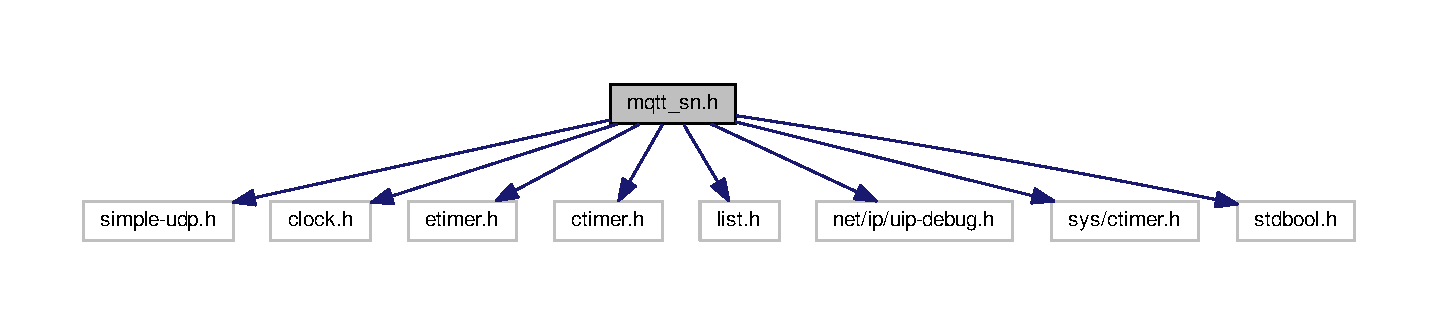
\includegraphics[width=350pt]{mqtt__sn_8h__incl}
\end{center}
\end{figure}
Este grafo mostra quais são os ficheiros que incluem directamente ou indirectamente este ficheiro\+:
\nopagebreak
\begin{figure}[H]
\begin{center}
\leavevmode
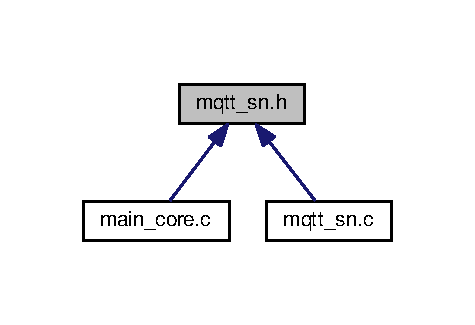
\includegraphics[width=228pt]{mqtt__sn_8h__dep__incl}
\end{center}
\end{figure}
\subsection*{Estruturas de Dados}
\begin{DoxyCompactItemize}
\item 
struct \hyperlink{structmqtt__sn__task__t}{mqtt\+\_\+sn\+\_\+task\+\_\+t}
\begin{DoxyCompactList}\small\item\em Estrutura de tarefa de fila M\+Q\+T\+T-\/\+S\+N. \end{DoxyCompactList}\item 
struct \hyperlink{structnode}{node}
\begin{DoxyCompactList}\small\item\em Estrutura de fila M\+Q\+T\+T-\/\+S\+N. \end{DoxyCompactList}\item 
struct \hyperlink{structshort__topics__t}{short\+\_\+topics\+\_\+t}
\item 
struct \hyperlink{structmqtt__sn__con__t}{mqtt\+\_\+sn\+\_\+con\+\_\+t}
\begin{DoxyCompactList}\small\item\em Estrutura de conexão ao broker M\+Q\+T\+T-\/\+S\+N. \end{DoxyCompactList}\end{DoxyCompactItemize}
\subsection*{Macros}
\begin{DoxyCompactItemize}
\item 
\#define \hyperlink{group__MQTT__SN__DEBUG_ga7871b41b94f3b5aac9e79ad353903ae7}{D\+E\+B\+U\+G\+\_\+\+O\+S}
\begin{DoxyCompactList}\small\item\em Se definida habilita mensagens de debug da rede M\+Q\+T\+T-\/\+S\+N. \end{DoxyCompactList}\item 
\hypertarget{group__MQTT__SN__DEBUG_gac3a54f3a6ca71cb643dc99df536f503c}{\#define \hyperlink{group__MQTT__SN__DEBUG_gac3a54f3a6ca71cb643dc99df536f503c}{D\+E\+B\+U\+G\+\_\+\+T\+A\+S\+K}}\label{group__MQTT__SN__DEBUG_gac3a54f3a6ca71cb643dc99df536f503c}

\begin{DoxyCompactList}\small\item\em Se definida habilita mensagens de debug de tarefas da fila utilizada pelo M\+Q\+T\+T-\/\+S\+N. \end{DoxyCompactList}\item 
\hypertarget{mqtt__sn_8h_a36f42ab727628183e36ec7de583bf61f}{\#define {\bfseries debug\+\_\+task}(fmt, args...)~printf(\char`\"{}\textbackslash{}n\mbox{[}Tarefa\mbox{]} \char`\"{}fmt, \#\#args)}\label{mqtt__sn_8h_a36f42ab727628183e36ec7de583bf61f}

\item 
\hypertarget{mqtt__sn_8h_a4414818dcd874c17a091c7a4d9f9ed37}{\#define {\bfseries debug\+\_\+os}(fmt, args...)~printf(\char`\"{}\textbackslash{}n\mbox{[}D\+E\+M\+O\mbox{]} \char`\"{}fmt, \#\#args)}\label{mqtt__sn_8h_a4414818dcd874c17a091c7a4d9f9ed37}

\item 
\hypertarget{mqtt__sn_8h_a6b56b0cf4db4d6361115528894f6d792}{\#define {\bfseries debug\+\_\+mqtt}(fmt,...)}\label{mqtt__sn_8h_a6b56b0cf4db4d6361115528894f6d792}

\item 
\hypertarget{mqtt__sn_8h_a0d5347618ab59b9090d2d4dfcaf37395}{\#define {\bfseries debug\+\_\+udp}(fmt,...)}\label{mqtt__sn_8h_a0d5347618ab59b9090d2d4dfcaf37395}

\item 
\hypertarget{group__MQTT__SN__CONTROL_gac6620fe642df6fedae5da980e3cc1685}{\#define {\bfseries M\+Q\+T\+T\+\_\+\+S\+N\+\_\+\+M\+A\+X\+\_\+\+P\+A\+C\+K\+E\+T\+\_\+\+L\+E\+N\+G\+T\+H}~(255)}\label{group__MQTT__SN__CONTROL_gac6620fe642df6fedae5da980e3cc1685}

\item 
\hypertarget{group__MQTT__SN__CONTROL_ga3dccee9ebffc9265d5c3cd3107ca601b}{\#define {\bfseries M\+Q\+T\+T\+\_\+\+S\+N\+\_\+\+M\+A\+X\+\_\+\+T\+O\+P\+I\+C\+\_\+\+L\+E\+N\+G\+T\+H}~(M\+Q\+T\+T\+\_\+\+S\+N\+\_\+\+M\+A\+X\+\_\+\+P\+A\+C\+K\+E\+T\+\_\+\+L\+E\+N\+G\+T\+H-\/6)}\label{group__MQTT__SN__CONTROL_ga3dccee9ebffc9265d5c3cd3107ca601b}

\item 
\hypertarget{group__MQTT__SN__CONTROL_ga064185df38354c8d31cba8f173a8b39f}{\#define {\bfseries M\+Q\+T\+T\+\_\+\+S\+N\+\_\+\+T\+Y\+P\+E\+\_\+\+A\+D\+V\+E\+R\+T\+I\+S\+E}~(0x00)}\label{group__MQTT__SN__CONTROL_ga064185df38354c8d31cba8f173a8b39f}

\item 
\hypertarget{group__MQTT__SN__CONTROL_ga8170ee7211bec9249606010e8af4765d}{\#define {\bfseries M\+Q\+T\+T\+\_\+\+S\+N\+\_\+\+T\+Y\+P\+E\+\_\+\+S\+E\+A\+R\+C\+H\+G\+W}~(0x01)}\label{group__MQTT__SN__CONTROL_ga8170ee7211bec9249606010e8af4765d}

\item 
\hypertarget{group__MQTT__SN__CONTROL_ga5be35929c3e372b4a2fed0e133be0e92}{\#define {\bfseries M\+Q\+T\+T\+\_\+\+S\+N\+\_\+\+T\+Y\+P\+E\+\_\+\+G\+W\+I\+N\+F\+O}~(0x02)}\label{group__MQTT__SN__CONTROL_ga5be35929c3e372b4a2fed0e133be0e92}

\item 
\hypertarget{group__MQTT__SN__CONTROL_ga0ad512804838d2ba709e82ffb010d991}{\#define {\bfseries M\+Q\+T\+T\+\_\+\+S\+N\+\_\+\+T\+Y\+P\+E\+\_\+\+C\+O\+N\+N\+E\+C\+T}~(0x04)}\label{group__MQTT__SN__CONTROL_ga0ad512804838d2ba709e82ffb010d991}

\item 
\hypertarget{group__MQTT__SN__CONTROL_gac4469be7c31731176bfa8c5bd38f3a58}{\#define {\bfseries M\+Q\+T\+T\+\_\+\+S\+N\+\_\+\+T\+Y\+P\+E\+\_\+\+C\+O\+N\+N\+A\+C\+K}~(0x05)}\label{group__MQTT__SN__CONTROL_gac4469be7c31731176bfa8c5bd38f3a58}

\item 
\hypertarget{group__MQTT__SN__CONTROL_ga914fff9b2b9e7c08d6b732599f0cf348}{\#define {\bfseries M\+Q\+T\+T\+\_\+\+S\+N\+\_\+\+T\+Y\+P\+E\+\_\+\+W\+I\+L\+L\+T\+O\+P\+I\+C\+R\+E\+Q}~(0x06)}\label{group__MQTT__SN__CONTROL_ga914fff9b2b9e7c08d6b732599f0cf348}

\item 
\hypertarget{group__MQTT__SN__CONTROL_ga95c657f75f0f02a093b8623a50dc0af8}{\#define {\bfseries M\+Q\+T\+T\+\_\+\+S\+N\+\_\+\+T\+Y\+P\+E\+\_\+\+W\+I\+L\+L\+T\+O\+P\+I\+C}~(0x07)}\label{group__MQTT__SN__CONTROL_ga95c657f75f0f02a093b8623a50dc0af8}

\item 
\hypertarget{group__MQTT__SN__CONTROL_gaefa36203de4d9ff51372abd51fa6521a}{\#define {\bfseries M\+Q\+T\+T\+\_\+\+S\+N\+\_\+\+T\+Y\+P\+E\+\_\+\+W\+I\+L\+L\+M\+S\+G\+R\+E\+Q}~(0x08)}\label{group__MQTT__SN__CONTROL_gaefa36203de4d9ff51372abd51fa6521a}

\item 
\hypertarget{group__MQTT__SN__CONTROL_ga0ab12c9559a2419e1c88080fa3c594c0}{\#define {\bfseries M\+Q\+T\+T\+\_\+\+S\+N\+\_\+\+T\+Y\+P\+E\+\_\+\+W\+I\+L\+L\+M\+S\+G}~(0x09)}\label{group__MQTT__SN__CONTROL_ga0ab12c9559a2419e1c88080fa3c594c0}

\item 
\hypertarget{group__MQTT__SN__CONTROL_ga742472508835bbeab8a22d6294f34e8f}{\#define {\bfseries M\+Q\+T\+T\+\_\+\+S\+N\+\_\+\+T\+Y\+P\+E\+\_\+\+R\+E\+G\+I\+S\+T\+E\+R}~(0x0\+A)}\label{group__MQTT__SN__CONTROL_ga742472508835bbeab8a22d6294f34e8f}

\item 
\hypertarget{group__MQTT__SN__CONTROL_gab600be8ae75c06a49cc89d0f7255ac12}{\#define {\bfseries M\+Q\+T\+T\+\_\+\+S\+N\+\_\+\+T\+Y\+P\+E\+\_\+\+R\+E\+G\+A\+C\+K}~(0x0\+B)}\label{group__MQTT__SN__CONTROL_gab600be8ae75c06a49cc89d0f7255ac12}

\item 
\hypertarget{group__MQTT__SN__CONTROL_ga1c34c285be401165ca3b9ef1c9180354}{\#define {\bfseries M\+Q\+T\+T\+\_\+\+S\+N\+\_\+\+T\+Y\+P\+E\+\_\+\+P\+U\+B\+L\+I\+S\+H}~(0x0\+C)}\label{group__MQTT__SN__CONTROL_ga1c34c285be401165ca3b9ef1c9180354}

\item 
\hypertarget{group__MQTT__SN__CONTROL_ga5bc44c53d2905a5242a3b72d44c125b2}{\#define {\bfseries M\+Q\+T\+T\+\_\+\+S\+N\+\_\+\+T\+Y\+P\+E\+\_\+\+P\+U\+B\+A\+C\+K}~(0x0\+D)}\label{group__MQTT__SN__CONTROL_ga5bc44c53d2905a5242a3b72d44c125b2}

\item 
\hypertarget{group__MQTT__SN__CONTROL_gacef39c4b8c3dd36ed4caf90f6a716585}{\#define {\bfseries M\+Q\+T\+T\+\_\+\+S\+N\+\_\+\+T\+Y\+P\+E\+\_\+\+P\+U\+B\+C\+O\+M\+P}~(0x0\+E)}\label{group__MQTT__SN__CONTROL_gacef39c4b8c3dd36ed4caf90f6a716585}

\item 
\hypertarget{group__MQTT__SN__CONTROL_gac4953c83079abc9804fce7dca7b0a648}{\#define {\bfseries M\+Q\+T\+T\+\_\+\+S\+N\+\_\+\+T\+Y\+P\+E\+\_\+\+P\+U\+B\+R\+E\+C}~(0x0\+F)}\label{group__MQTT__SN__CONTROL_gac4953c83079abc9804fce7dca7b0a648}

\item 
\hypertarget{group__MQTT__SN__CONTROL_ga74daeb038d5cf996c680fc34b187dfba}{\#define {\bfseries M\+Q\+T\+T\+\_\+\+S\+N\+\_\+\+T\+Y\+P\+E\+\_\+\+P\+U\+B\+R\+E\+L}~(0x10)}\label{group__MQTT__SN__CONTROL_ga74daeb038d5cf996c680fc34b187dfba}

\item 
\hypertarget{group__MQTT__SN__CONTROL_ga1e4f5d7bc584d5ffcda760303ab76904}{\#define {\bfseries M\+Q\+T\+T\+\_\+\+S\+N\+\_\+\+T\+Y\+P\+E\+\_\+\+S\+U\+B\+S\+C\+R\+I\+B\+E}~(0x12)}\label{group__MQTT__SN__CONTROL_ga1e4f5d7bc584d5ffcda760303ab76904}

\item 
\hypertarget{group__MQTT__SN__CONTROL_ga6db4e874ad63924de121a89d4bcd559d}{\#define {\bfseries M\+Q\+T\+T\+\_\+\+S\+N\+\_\+\+T\+Y\+P\+E\+\_\+\+S\+U\+B\+A\+C\+K}~(0x13)}\label{group__MQTT__SN__CONTROL_ga6db4e874ad63924de121a89d4bcd559d}

\item 
\hypertarget{group__MQTT__SN__CONTROL_ga0aaddbe1b0ebd1ece45ada17e618e560}{\#define {\bfseries M\+Q\+T\+T\+\_\+\+S\+N\+\_\+\+T\+Y\+P\+E\+\_\+\+U\+N\+S\+U\+B\+S\+C\+R\+I\+B\+E}~(0x14)}\label{group__MQTT__SN__CONTROL_ga0aaddbe1b0ebd1ece45ada17e618e560}

\item 
\hypertarget{group__MQTT__SN__CONTROL_ga494ee75d7c290823f3738a4d77beea97}{\#define {\bfseries M\+Q\+T\+T\+\_\+\+S\+N\+\_\+\+T\+Y\+P\+E\+\_\+\+U\+N\+S\+U\+B\+A\+C\+K}~(0x15)}\label{group__MQTT__SN__CONTROL_ga494ee75d7c290823f3738a4d77beea97}

\item 
\hypertarget{group__MQTT__SN__CONTROL_ga24c4412f26f5db3dabc57c8511690a7b}{\#define {\bfseries M\+Q\+T\+T\+\_\+\+S\+N\+\_\+\+T\+Y\+P\+E\+\_\+\+P\+I\+N\+G\+R\+E\+Q}~(0x16)}\label{group__MQTT__SN__CONTROL_ga24c4412f26f5db3dabc57c8511690a7b}

\item 
\hypertarget{group__MQTT__SN__CONTROL_ga104849c06dad11e57805341ca6394513}{\#define {\bfseries M\+Q\+T\+T\+\_\+\+S\+N\+\_\+\+T\+Y\+P\+E\+\_\+\+P\+I\+N\+G\+R\+E\+S\+P}~(0x17)}\label{group__MQTT__SN__CONTROL_ga104849c06dad11e57805341ca6394513}

\item 
\hypertarget{group__MQTT__SN__CONTROL_gaeb18a759d020c1443a602636204c6fdd}{\#define {\bfseries M\+Q\+T\+T\+\_\+\+S\+N\+\_\+\+T\+Y\+P\+E\+\_\+\+D\+I\+S\+C\+O\+N\+N\+E\+C\+T}~(0x18)}\label{group__MQTT__SN__CONTROL_gaeb18a759d020c1443a602636204c6fdd}

\item 
\hypertarget{group__MQTT__SN__CONTROL_gae34bbdc05e79d37cc1f2060a885c3e05}{\#define {\bfseries M\+Q\+T\+T\+\_\+\+S\+N\+\_\+\+T\+Y\+P\+E\+\_\+\+W\+I\+L\+L\+T\+O\+P\+I\+C\+U\+P\+D}~(0x1\+A)}\label{group__MQTT__SN__CONTROL_gae34bbdc05e79d37cc1f2060a885c3e05}

\item 
\hypertarget{group__MQTT__SN__CONTROL_ga3181a18a9d476f1ca97a1bc935c8b712}{\#define {\bfseries M\+Q\+T\+T\+\_\+\+S\+N\+\_\+\+T\+Y\+P\+E\+\_\+\+W\+I\+L\+L\+T\+O\+P\+I\+C\+R\+E\+S\+P}~(0x1\+B)}\label{group__MQTT__SN__CONTROL_ga3181a18a9d476f1ca97a1bc935c8b712}

\item 
\hypertarget{group__MQTT__SN__CONTROL_ga63c970e654cb17f2a30294a719b11b71}{\#define {\bfseries M\+Q\+T\+T\+\_\+\+S\+N\+\_\+\+T\+Y\+P\+E\+\_\+\+W\+I\+L\+L\+M\+S\+G\+U\+P\+D}~(0x1\+C)}\label{group__MQTT__SN__CONTROL_ga63c970e654cb17f2a30294a719b11b71}

\item 
\hypertarget{group__MQTT__SN__CONTROL_ga855273768c5808acc67a07b8c4b6f5fa}{\#define {\bfseries M\+Q\+T\+T\+\_\+\+S\+N\+\_\+\+T\+Y\+P\+E\+\_\+\+W\+I\+L\+L\+M\+S\+G\+R\+E\+S\+P}~(0x1\+D)}\label{group__MQTT__SN__CONTROL_ga855273768c5808acc67a07b8c4b6f5fa}

\item 
\hypertarget{group__MQTT__SN__CONTROL_gaccc43fa2c1468ee81b07ca73265057e0}{\#define {\bfseries M\+Q\+T\+T\+\_\+\+S\+N\+\_\+\+T\+Y\+P\+E\+\_\+\+S\+U\+B\+\_\+\+W\+I\+L\+D\+C\+A\+R\+D}~(0x1\+E)}\label{group__MQTT__SN__CONTROL_gaccc43fa2c1468ee81b07ca73265057e0}

\item 
\hypertarget{group__MQTT__SN__CONTROL_ga206c51c6b01cdf9347809ebfc03caaef}{\#define {\bfseries M\+Q\+T\+T\+\_\+\+S\+N\+\_\+\+T\+O\+P\+I\+C\+\_\+\+T\+Y\+P\+E\+\_\+\+N\+O\+R\+M\+A\+L}~(0x00)}\label{group__MQTT__SN__CONTROL_ga206c51c6b01cdf9347809ebfc03caaef}

\item 
\hypertarget{group__MQTT__SN__CONTROL_ga655ae15e8e7734cedf42fab6eb3610b5}{\#define {\bfseries M\+Q\+T\+T\+\_\+\+S\+N\+\_\+\+T\+O\+P\+I\+C\+\_\+\+T\+Y\+P\+E\+\_\+\+P\+R\+E\+D\+E\+F\+I\+N\+E\+D}~(0x01)}\label{group__MQTT__SN__CONTROL_ga655ae15e8e7734cedf42fab6eb3610b5}

\item 
\hypertarget{group__MQTT__SN__CONTROL_gaa17c2076a81b61d2719199521563d1c5}{\#define {\bfseries M\+Q\+T\+T\+\_\+\+S\+N\+\_\+\+T\+O\+P\+I\+C\+\_\+\+T\+Y\+P\+E\+\_\+\+S\+H\+O\+R\+T}~(0x02)}\label{group__MQTT__SN__CONTROL_gaa17c2076a81b61d2719199521563d1c5}

\item 
\hypertarget{group__MQTT__SN__CONTROL_ga2d49bf6469a7864f24a537f059ee0612}{\#define {\bfseries M\+Q\+T\+T\+\_\+\+S\+N\+\_\+\+F\+L\+A\+G\+\_\+\+D\+U\+P}~(0x1 $<$$<$ 7)}\label{group__MQTT__SN__CONTROL_ga2d49bf6469a7864f24a537f059ee0612}

\item 
\hypertarget{group__MQTT__SN__CONTROL_ga37b57822f47fbb4ba1639e5be988c437}{\#define {\bfseries M\+Q\+T\+T\+\_\+\+S\+N\+\_\+\+F\+L\+A\+G\+\_\+\+Q\+O\+S\+\_\+0}~(0x0 $<$$<$ 5)}\label{group__MQTT__SN__CONTROL_ga37b57822f47fbb4ba1639e5be988c437}

\item 
\hypertarget{group__MQTT__SN__CONTROL_ga6d04b90ba54b58e08caa593a84105f21}{\#define {\bfseries M\+Q\+T\+T\+\_\+\+S\+N\+\_\+\+F\+L\+A\+G\+\_\+\+Q\+O\+S\+\_\+1}~(0x1 $<$$<$ 5)}\label{group__MQTT__SN__CONTROL_ga6d04b90ba54b58e08caa593a84105f21}

\item 
\hypertarget{group__MQTT__SN__CONTROL_ga953eaf715ee6055e9f119950be8d7399}{\#define {\bfseries M\+Q\+T\+T\+\_\+\+S\+N\+\_\+\+F\+L\+A\+G\+\_\+\+Q\+O\+S\+\_\+2}~(0x2 $<$$<$ 5)}\label{group__MQTT__SN__CONTROL_ga953eaf715ee6055e9f119950be8d7399}

\item 
\hypertarget{group__MQTT__SN__CONTROL_ga8095eefa31299b606b4ba8bbbcb00195}{\#define {\bfseries M\+Q\+T\+T\+\_\+\+S\+N\+\_\+\+F\+L\+A\+G\+\_\+\+Q\+O\+S\+\_\+\+N1}~(0x3 $<$$<$ 5)}\label{group__MQTT__SN__CONTROL_ga8095eefa31299b606b4ba8bbbcb00195}

\item 
\hypertarget{group__MQTT__SN__CONTROL_ga45271b87fd548295bc4c86c225fc648e}{\#define {\bfseries M\+Q\+T\+T\+\_\+\+S\+N\+\_\+\+F\+L\+A\+G\+\_\+\+R\+E\+T\+A\+I\+N}~(0x1 $<$$<$ 4)}\label{group__MQTT__SN__CONTROL_ga45271b87fd548295bc4c86c225fc648e}

\item 
\hypertarget{group__MQTT__SN__CONTROL_ga8e3f7578e0fef59224e365cef8613f8e}{\#define {\bfseries M\+Q\+T\+T\+\_\+\+S\+N\+\_\+\+F\+L\+A\+G\+\_\+\+W\+I\+L\+L}~(0x1 $<$$<$ 3)}\label{group__MQTT__SN__CONTROL_ga8e3f7578e0fef59224e365cef8613f8e}

\item 
\hypertarget{group__MQTT__SN__CONTROL_ga842ab1c7124c0b63f62ed3283dafbe06}{\#define {\bfseries M\+Q\+T\+T\+\_\+\+S\+N\+\_\+\+F\+L\+A\+G\+\_\+\+C\+L\+E\+A\+N}~(0x1 $<$$<$ 2)}\label{group__MQTT__SN__CONTROL_ga842ab1c7124c0b63f62ed3283dafbe06}

\item 
\hypertarget{group__MQTT__SN__CONTROL_ga0066dd4afeef507b2e8f5ac01f71ea37}{\#define {\bfseries M\+Q\+T\+T\+\_\+\+S\+N\+\_\+\+P\+R\+O\+T\+O\+C\+O\+L\+\_\+\+I\+D}~(0x01)}\label{group__MQTT__SN__CONTROL_ga0066dd4afeef507b2e8f5ac01f71ea37}

\item 
\hypertarget{group__MQTT__SN__CONTROL_ga43005b6b1934800f67a6d169c779c92b}{\#define {\bfseries A\+C\+C\+E\+P\+T\+E\+D}~0x00}\label{group__MQTT__SN__CONTROL_ga43005b6b1934800f67a6d169c779c92b}

\item 
\hypertarget{group__MQTT__SN__CONTROL_ga9b2b214d1ddb0f617efdd26ccc91def4}{\#define {\bfseries R\+E\+J\+E\+C\+T\+E\+D\+\_\+\+C\+O\+N\+G\+E\+S\+T\+I\+O\+N}~0x01}\label{group__MQTT__SN__CONTROL_ga9b2b214d1ddb0f617efdd26ccc91def4}

\item 
\hypertarget{group__MQTT__SN__CONTROL_ga9b548f6c60530b07c9b9f5ef5b1ac8b9}{\#define {\bfseries R\+E\+J\+E\+C\+T\+E\+D\+\_\+\+I\+N\+V\+A\+L\+I\+D\+\_\+\+T\+O\+P\+I\+C\+\_\+\+I\+D}~0x02}\label{group__MQTT__SN__CONTROL_ga9b548f6c60530b07c9b9f5ef5b1ac8b9}

\item 
\hypertarget{group__MQTT__SN__CONTROL_ga93af4e6b658c4823ae9603b86bb7c64a}{\#define {\bfseries R\+E\+J\+E\+C\+T\+E\+D\+\_\+\+N\+O\+T\+\_\+\+S\+U\+P\+P\+O\+R\+T\+E\+D}~0x03}\label{group__MQTT__SN__CONTROL_ga93af4e6b658c4823ae9603b86bb7c64a}

\item 
\hypertarget{group__MQTT__SN__CONTROL_ga206c51c6b01cdf9347809ebfc03caaef}{\#define {\bfseries M\+Q\+T\+T\+\_\+\+S\+N\+\_\+\+T\+O\+P\+I\+C\+\_\+\+T\+Y\+P\+E\+\_\+\+N\+O\+R\+M\+A\+L}~(0x00)}\label{group__MQTT__SN__CONTROL_ga206c51c6b01cdf9347809ebfc03caaef}

\item 
\hypertarget{group__MQTT__SN__CONTROL_ga655ae15e8e7734cedf42fab6eb3610b5}{\#define {\bfseries M\+Q\+T\+T\+\_\+\+S\+N\+\_\+\+T\+O\+P\+I\+C\+\_\+\+T\+Y\+P\+E\+\_\+\+P\+R\+E\+D\+E\+F\+I\+N\+E\+D}~(0x01)}\label{group__MQTT__SN__CONTROL_ga655ae15e8e7734cedf42fab6eb3610b5}

\item 
\hypertarget{group__MQTT__SN__CONTROL_gaa17c2076a81b61d2719199521563d1c5}{\#define {\bfseries M\+Q\+T\+T\+\_\+\+S\+N\+\_\+\+T\+O\+P\+I\+C\+\_\+\+T\+Y\+P\+E\+\_\+\+S\+H\+O\+R\+T}~(0x02)}\label{group__MQTT__SN__CONTROL_gaa17c2076a81b61d2719199521563d1c5}

\item 
\hypertarget{group__MQTT__SN__CONTROL_ga34bf6ae7cc029057c70910ae26a3335f}{\#define \hyperlink{group__MQTT__SN__CONTROL_ga34bf6ae7cc029057c70910ae26a3335f}{ss}(x)~sizeof(x)/sizeof($\ast$x)}\label{group__MQTT__SN__CONTROL_ga34bf6ae7cc029057c70910ae26a3335f}

\begin{DoxyCompactList}\small\item\em Computa o tamanho de um vetor de ponteiros. \end{DoxyCompactList}\item 
\hypertarget{group__MQTT__SN__CONTROL_ga8d316cee94174b8c2d16e328fdf1e607}{\#define \hyperlink{group__MQTT__SN__CONTROL_ga8d316cee94174b8c2d16e328fdf1e607}{M\+Q\+T\+T\+\_\+\+S\+N\+\_\+\+A\+U\+T\+O\+\_\+\+R\+E\+C\+O\+N\+N\+E\+C\+T}}\label{group__MQTT__SN__CONTROL_ga8d316cee94174b8c2d16e328fdf1e607}

\begin{DoxyCompactList}\small\item\em Define se o dispositivo deve se auto conectar de tempos em tempos. \end{DoxyCompactList}\item 
\hypertarget{group__MQTT__SN__CONTROL_ga180af20d177732dc470c147452feb30f}{\#define \hyperlink{group__MQTT__SN__CONTROL_ga180af20d177732dc470c147452feb30f}{M\+Q\+T\+T\+\_\+\+S\+N\+\_\+\+R\+E\+T\+R\+Y\+\_\+\+P\+I\+N\+G}~5}\label{group__MQTT__SN__CONTROL_ga180af20d177732dc470c147452feb30f}

\begin{DoxyCompactList}\small\item\em Número de tentativas de envio de P\+I\+N\+G R\+E\+Q\+U\+E\+S\+T antes de desconectar nó $<$-\/$>$ broker. \end{DoxyCompactList}\item 
\hypertarget{group__MQTT__SN__CONTROL_ga7533efb537d4d4eebf1b6d3d5256cb0b}{\#define \hyperlink{group__MQTT__SN__CONTROL_ga7533efb537d4d4eebf1b6d3d5256cb0b}{M\+Q\+T\+T\+\_\+\+S\+N\+\_\+\+T\+I\+M\+E\+O\+U\+T\+\_\+\+C\+O\+N\+N\+E\+C\+T}~9$\ast$C\+L\+O\+C\+K\+\_\+\+S\+E\+C\+O\+N\+D}\label{group__MQTT__SN__CONTROL_ga7533efb537d4d4eebf1b6d3d5256cb0b}

\begin{DoxyCompactList}\small\item\em Tempo base para comunicação M\+Q\+T\+T-\/\+S\+N broker $<$-\/$>$ nó \end{DoxyCompactList}\item 
\hypertarget{group__MQTT__SN__CONTROL_ga47da8d46176b160b0db00fe221725d4c}{\#define \hyperlink{group__MQTT__SN__CONTROL_ga47da8d46176b160b0db00fe221725d4c}{M\+Q\+T\+T\+\_\+\+S\+N\+\_\+\+T\+I\+M\+E\+O\+U\+T}~C\+L\+O\+C\+K\+\_\+\+S\+E\+C\+O\+N\+D}\label{group__MQTT__SN__CONTROL_ga47da8d46176b160b0db00fe221725d4c}

\begin{DoxyCompactList}\small\item\em Tempo base para comunicação M\+Q\+T\+T-\/\+S\+N broker $<$-\/$>$ nó \end{DoxyCompactList}\item 
\hypertarget{group__MQTT__SN__CONTROL_gaad5ac7de3008d8fa37447193aebc31e2}{\#define \hyperlink{group__MQTT__SN__CONTROL_gaad5ac7de3008d8fa37447193aebc31e2}{M\+Q\+T\+T\+\_\+\+S\+N\+\_\+\+R\+E\+T\+R\+Y}~5}\label{group__MQTT__SN__CONTROL_gaad5ac7de3008d8fa37447193aebc31e2}

\begin{DoxyCompactList}\small\item\em Número de tentativas de enviar qualquer pacote ao broker antes de desconectar. \end{DoxyCompactList}\item 
\hypertarget{group__MQTT__SN__CONTROL_ga45ab5881e190d570f3784e50be2cce65}{\#define \hyperlink{group__MQTT__SN__CONTROL_ga45ab5881e190d570f3784e50be2cce65}{M\+A\+X\+\_\+\+Q\+U\+E\+U\+E\+\_\+\+M\+Q\+T\+T\+\_\+\+S\+N}~100}\label{group__MQTT__SN__CONTROL_ga45ab5881e190d570f3784e50be2cce65}

\begin{DoxyCompactList}\small\item\em Número máximo de tarefas a serem inseridas alocadas dinamicamente M\+Q\+T\+T-\/\+S\+N. \end{DoxyCompactList}\item 
\hypertarget{group__MQTT__SN__CONTROL_ga5ed98e8fc00194886ebc14d25540f81b}{\#define \hyperlink{group__MQTT__SN__CONTROL_ga5ed98e8fc00194886ebc14d25540f81b}{M\+A\+X\+\_\+\+T\+O\+P\+I\+C\+\_\+\+U\+S\+E\+D}~100}\label{group__MQTT__SN__CONTROL_ga5ed98e8fc00194886ebc14d25540f81b}

\begin{DoxyCompactList}\small\item\em Número máximo de tópicos que o usuário pode registrar, a A\+P\+I cria um conjunto de estruturas para o bind de topic e short topic id. \end{DoxyCompactList}\end{DoxyCompactItemize}
\subsection*{Definições de tipos}
\begin{DoxyCompactItemize}
\item 
\hypertarget{mqtt__sn_8h_a679e4bebc7798d960960760150bdc5a7}{typedef void($\ast$ \hyperlink{mqtt__sn_8h_a679e4bebc7798d960960760150bdc5a7}{mqtt\+\_\+sn\+\_\+cb\+\_\+f} )(char $\ast$, char $\ast$)}\label{mqtt__sn_8h_a679e4bebc7798d960960760150bdc5a7}

\begin{DoxyCompactList}\small\item\em Tipo de função de callback que deve ser repassada ao broker. \end{DoxyCompactList}\item 
\hypertarget{mqtt__sn_8h_add91ba4199db8665b9b9fc56fc6783a6}{typedef enum \hyperlink{mqtt__sn_8h_a754c1055b4431040415cf01b39caaa98}{resp\+\_\+con} \hyperlink{mqtt__sn_8h_add91ba4199db8665b9b9fc56fc6783a6}{resp\+\_\+con\+\_\+t}}\label{mqtt__sn_8h_add91ba4199db8665b9b9fc56fc6783a6}

\begin{DoxyCompactList}\small\item\em Tipo de erros de funções. \end{DoxyCompactList}\end{DoxyCompactItemize}
\subsection*{Enumerações}
\begin{DoxyCompactItemize}
\item 
enum \hyperlink{mqtt__sn_8h_a754c1055b4431040415cf01b39caaa98}{resp\+\_\+con} \{ \hyperlink{mqtt__sn_8h_a754c1055b4431040415cf01b39caaa98ac6ae922662cbaf7958eb387bfd6fe4da}{F\+A\+I\+L\+\_\+\+C\+O\+N}, 
\hyperlink{mqtt__sn_8h_a754c1055b4431040415cf01b39caaa98ae7b7a388c90c2c5428cced225760885f}{S\+U\+C\+C\+E\+S\+S\+\_\+\+C\+O\+N}
 \}
\item 
\hypertarget{mqtt__sn_8h_aab2bca192b63f37bf4847be3686bca75}{enum \hyperlink{mqtt__sn_8h_aab2bca192b63f37bf4847be3686bca75}{mqtt\+\_\+sn\+\_\+status\+\_\+t} \{ \\*
{\bfseries M\+Q\+T\+T\+S\+N\+\_\+\+C\+O\+N\+N\+E\+C\+T\+I\+O\+N\+\_\+\+F\+A\+I\+L\+E\+D}, 
{\bfseries M\+Q\+T\+T\+S\+N\+\_\+\+D\+I\+S\+C\+O\+N\+N\+E\+C\+T\+E\+D}, 
{\bfseries M\+Q\+T\+T\+S\+N\+\_\+\+W\+A\+I\+T\+I\+N\+G\+\_\+\+C\+O\+N\+N\+A\+C\+K}, 
{\bfseries M\+Q\+T\+T\+S\+N\+\_\+\+W\+A\+I\+T\+I\+N\+G\+\_\+\+W\+I\+L\+L\+T\+O\+P\+I\+C\+R\+E\+Q}, 
\\*
{\bfseries M\+Q\+T\+T\+S\+N\+\_\+\+W\+A\+I\+T\+I\+N\+G\+\_\+\+W\+I\+L\+L\+M\+S\+G\+R\+E\+Q}, 
{\bfseries M\+Q\+T\+T\+S\+N\+\_\+\+W\+A\+I\+T\+I\+N\+G\+\_\+\+R\+E\+G\+A\+C\+K}, 
{\bfseries M\+Q\+T\+T\+S\+N\+\_\+\+C\+O\+N\+N\+E\+C\+T\+E\+D}, 
{\bfseries M\+Q\+T\+T\+S\+N\+\_\+\+T\+O\+P\+I\+C\+\_\+\+R\+E\+G\+I\+S\+T\+E\+R\+E\+D}, 
\\*
{\bfseries M\+Q\+T\+T\+S\+N\+\_\+\+T\+O\+P\+I\+C\+\_\+\+S\+U\+B\+S\+C\+R\+I\+B\+I\+N\+G}, 
{\bfseries M\+Q\+T\+T\+S\+N\+\_\+\+W\+A\+I\+T\+I\+N\+G\+\_\+\+P\+U\+B\+A\+C\+K}, 
{\bfseries M\+Q\+T\+T\+S\+N\+\_\+\+W\+A\+I\+T\+I\+N\+G\+\_\+\+S\+U\+B\+A\+C\+K}, 
{\bfseries M\+Q\+T\+T\+S\+N\+\_\+\+P\+U\+B\+\_\+\+R\+E\+Q}, 
\\*
{\bfseries M\+Q\+T\+T\+S\+N\+\_\+\+S\+U\+B\+\_\+\+R\+E\+Q}, 
{\bfseries M\+Q\+T\+T\+S\+N\+\_\+\+R\+E\+G\+\_\+\+R\+E\+Q}
 \}}\label{mqtt__sn_8h_aab2bca192b63f37bf4847be3686bca75}

\begin{DoxyCompactList}\small\item\em Estados da A\+S\+M do M\+Q\+T\+T-\/\+S\+N. \end{DoxyCompactList}\end{DoxyCompactItemize}
\subsection*{Funções}
\begin{DoxyCompactItemize}
\item 
\hypertarget{group__Pacotes_gab898071398b359603a35c202e9c65f3b}{struct {\bfseries \+\_\+\+\_\+attribute\+\_\+\+\_\+} ((packed))}\label{group__Pacotes_gab898071398b359603a35c202e9c65f3b}

\item 
\hyperlink{mqtt__sn_8h_add91ba4199db8665b9b9fc56fc6783a6}{resp\+\_\+con\+\_\+t} \hyperlink{mqtt__sn_8h_a575514d0f0fd3b6c5c4a2c75e604bf79}{mqtt\+\_\+sn\+\_\+insert\+\_\+queue} (\hyperlink{structmqtt__sn__task__t}{mqtt\+\_\+sn\+\_\+task\+\_\+t} new)
\begin{DoxyCompactList}\small\item\em Insere uma tarefa na fila. \end{DoxyCompactList}\item 
void \hyperlink{mqtt__sn_8h_ad0a729c99366dad086be6be954e71f2c}{mqtt\+\_\+sn\+\_\+delete\+\_\+queue} ()
\begin{DoxyCompactList}\small\item\em Remove o elemento mais próximo de ser processado. \end{DoxyCompactList}\item 
void \hyperlink{mqtt__sn_8h_a71004d5b7e8b1add14024102d8d62042}{mqtt\+\_\+sn\+\_\+check\+\_\+queue} ()
\begin{DoxyCompactList}\small\item\em Lista as tarefas da fila. \end{DoxyCompactList}\item 
\hyperlink{mqtt__sn_8h_add91ba4199db8665b9b9fc56fc6783a6}{resp\+\_\+con\+\_\+t} \hyperlink{mqtt__sn_8h_a172afa34fe10ad1ee4ffc0d226b35b4d}{mqtt\+\_\+sn\+\_\+check\+\_\+rc} (uint8\+\_\+t rc)
\begin{DoxyCompactList}\small\item\em Envia requisição de conexão ao broker M\+Q\+T\+T-\/\+S\+N. \end{DoxyCompactList}\item 
void \hyperlink{mqtt__sn_8h_af9146fa082fe2bc6612fb13dbb20ed36}{mqtt\+\_\+sn\+\_\+recv\+\_\+parser} (const uint8\+\_\+t $\ast$data)
\begin{DoxyCompactList}\small\item\em Realiza o parsing das mensagens U\+D\+P recebidas. \end{DoxyCompactList}\item 
\hyperlink{mqtt__sn_8h_add91ba4199db8665b9b9fc56fc6783a6}{resp\+\_\+con\+\_\+t} \hyperlink{mqtt__sn_8h_a8771e78d9d8d5379ff27fba1feefe37c}{mqtt\+\_\+sn\+\_\+create\+\_\+sck} (\hyperlink{structmqtt__sn__con__t}{mqtt\+\_\+sn\+\_\+con\+\_\+t} mqtt\+\_\+sn\+\_\+connection, char $\ast$topics\mbox{[}$\,$\mbox{]}, size\+\_\+t topic\+\_\+len, \hyperlink{mqtt__sn_8h_a679e4bebc7798d960960760150bdc5a7}{mqtt\+\_\+sn\+\_\+cb\+\_\+f} cb\+\_\+f)
\begin{DoxyCompactList}\small\item\em Inicia conexão ao broker U\+D\+P. \end{DoxyCompactList}\item 
\hyperlink{mqtt__sn_8h_add91ba4199db8665b9b9fc56fc6783a6}{resp\+\_\+con\+\_\+t} \hyperlink{mqtt__sn_8h_ae17664af7f894e29743fafdf8bf98f89}{mqtt\+\_\+sn\+\_\+reg\+\_\+send} (void)
\begin{DoxyCompactList}\small\item\em Envio de mensagens ao broker do tipo R\+E\+G\+I\+S\+T\+E\+R. \end{DoxyCompactList}\item 
\hyperlink{mqtt__sn_8h_aab2bca192b63f37bf4847be3686bca75}{mqtt\+\_\+sn\+\_\+status\+\_\+t} \hyperlink{mqtt__sn_8h_a200e89a8fd400c652431bd505de6f827}{mqtt\+\_\+sn\+\_\+check\+\_\+status} (void)
\begin{DoxyCompactList}\small\item\em Checa o status da conexão M\+Q\+T\+T-\/\+S\+N. \end{DoxyCompactList}\item 
\hyperlink{mqtt__sn_8h_add91ba4199db8665b9b9fc56fc6783a6}{resp\+\_\+con\+\_\+t} \hyperlink{mqtt__sn_8h_a1b8eb51076a2923f2c036f1ff925c168}{mqtt\+\_\+sn\+\_\+con\+\_\+send} (void)
\begin{DoxyCompactList}\small\item\em Envia requisição de conexão ao broker M\+Q\+T\+T-\/\+S\+N. \end{DoxyCompactList}\item 
bool \hyperlink{mqtt__sn_8h_afb698c97e10afa31e2c11351f6ce9388}{mqtt\+\_\+sn\+\_\+check\+\_\+empty} (void)
\begin{DoxyCompactList}\small\item\em Checa o status da fila de tarefas M\+Q\+T\+T-\/\+S\+N. \end{DoxyCompactList}\item 
void \hyperlink{mqtt__sn_8h_ac598f98e844bfd5bbdb577099ddf06d1}{parse\+\_\+mqtt\+\_\+type\+\_\+string} (uint8\+\_\+t type, char $\ast$$\ast$type\+\_\+string)
\begin{DoxyCompactList}\small\item\em Retorna a string de status correspondente. \end{DoxyCompactList}\item 
void \hyperlink{mqtt__sn_8h_a46fe607d1db728d41ed6aec6fee3fc77}{mqtt\+\_\+sn\+\_\+init} (void)
\begin{DoxyCompactList}\small\item\em Inicializa P\+R\+O\+C\+E\+S\+S\+\_\+\+T\+H\+R\+E\+A\+D M\+Q\+T\+T-\/\+S\+N. \end{DoxyCompactList}\item 
\hyperlink{mqtt__sn_8h_add91ba4199db8665b9b9fc56fc6783a6}{resp\+\_\+con\+\_\+t} \hyperlink{mqtt__sn_8h_a550856b818c23fce9e4d5b253c3e7547}{mqtt\+\_\+sn\+\_\+pub\+\_\+send} (char $\ast$topic, char $\ast$message, bool retain\+\_\+flag, uint8\+\_\+t qos)
\begin{DoxyCompactList}\small\item\em Envia pacote P\+U\+B\+L\+I\+S\+H ao broker M\+Q\+T\+T-\/\+S\+N. \end{DoxyCompactList}\item 
char $\ast$ \hyperlink{mqtt__sn_8h_a9bd6d4e9304d00d28861751c22b146e4}{mqtt\+\_\+sn\+\_\+check\+\_\+status\+\_\+string} (void)
\begin{DoxyCompactList}\small\item\em Checa o status da conexãoe em String. \end{DoxyCompactList}\item 
uint8\+\_\+t \hyperlink{mqtt__sn_8h_adba0283cc8fadf24f2f04246c76e8cde}{mqtt\+\_\+sn\+\_\+get\+\_\+qos\+\_\+flag} (int8\+\_\+t qos)
\begin{DoxyCompactList}\small\item\em Gera a flag de nível Qo\+S. \end{DoxyCompactList}\item 
\hyperlink{mqtt__sn_8h_add91ba4199db8665b9b9fc56fc6783a6}{resp\+\_\+con\+\_\+t} \hyperlink{mqtt__sn_8h_ab8c0f238b41b373afb8b21e0f594b79d}{mqtt\+\_\+sn\+\_\+pub} (char $\ast$topic, char $\ast$message, bool retain\+\_\+flag, uint8\+\_\+t qos)
\begin{DoxyCompactList}\small\item\em Prepara requisição de publicação ao broker M\+Q\+T\+T-\/\+S\+N. \end{DoxyCompactList}\item 
void \hyperlink{mqtt__sn_8h_a6674e1ecf45890d3a15ab667fe4a4f58}{print\+\_\+g\+\_\+topics} (void)
\begin{DoxyCompactList}\small\item\em Exibe os tópicos registrados. \end{DoxyCompactList}\item 
void \hyperlink{mqtt__sn_8h_ac9614aca44158215c43b8810e052939d}{timeout\+\_\+con} (void $\ast$ptr)
\begin{DoxyCompactList}\small\item\em Processa timeout de pacotes. \end{DoxyCompactList}\item 
void \hyperlink{mqtt__sn_8h_a35dbd49b5fdc1d6e3dfe2b2d7255cf3e}{timeout\+\_\+ping\+\_\+mqtt} (void $\ast$ptr)
\begin{DoxyCompactList}\small\item\em Processa timeout de ping. \end{DoxyCompactList}\item 
void \hyperlink{mqtt__sn_8h_af09083ea59a182fdf109b6e3fa213bec}{mqtt\+\_\+sn\+\_\+ping\+\_\+send} (void)
\begin{DoxyCompactList}\small\item\em Envia requisição de ping ao broker. \end{DoxyCompactList}\item 
bool \hyperlink{mqtt__sn_8h_a2620f37584b501fde35e71806a78b35a}{unlock\+\_\+tasks} (void)
\begin{DoxyCompactList}\small\item\em Libera opção de geração de tarefas. \end{DoxyCompactList}\item 
\hyperlink{mqtt__sn_8h_add91ba4199db8665b9b9fc56fc6783a6}{resp\+\_\+con\+\_\+t} \hyperlink{mqtt__sn_8h_aab8d5db0224c9b083af9f18094053795}{mqtt\+\_\+sn\+\_\+sub} (char $\ast$topic, uint8\+\_\+t qos)
\begin{DoxyCompactList}\small\item\em Prepara requisição de inscrição ao broker M\+Q\+T\+T-\/\+S\+N. \end{DoxyCompactList}\item 
\hyperlink{mqtt__sn_8h_add91ba4199db8665b9b9fc56fc6783a6}{resp\+\_\+con\+\_\+t} \hyperlink{mqtt__sn_8h_a105b8d440266b4a582f2d627e57be14a}{mqtt\+\_\+sn\+\_\+sub\+\_\+send} (char $\ast$topic, uint8\+\_\+t qos)
\begin{DoxyCompactList}\small\item\em Envia pacote S\+U\+B\+S\+C\+R\+I\+B\+E ao broker M\+Q\+T\+T-\/\+S\+N. \end{DoxyCompactList}\item 
\hyperlink{mqtt__sn_8h_add91ba4199db8665b9b9fc56fc6783a6}{resp\+\_\+con\+\_\+t} \hyperlink{mqtt__sn_8h_a831d03a2cd7fbc884cec2013c2ebc823}{mqtt\+\_\+sn\+\_\+sub\+\_\+send\+\_\+wildcard} (char $\ast$topic, uint8\+\_\+t qos)
\begin{DoxyCompactList}\small\item\em Envia pacote S\+U\+B\+S\+C\+R\+I\+B\+E do tipo W\+I\+L\+D\+C\+A\+R\+D ao broker M\+Q\+T\+T-\/\+S\+N. \end{DoxyCompactList}\item 
\hyperlink{mqtt__sn_8h_add91ba4199db8665b9b9fc56fc6783a6}{resp\+\_\+con\+\_\+t} \hyperlink{mqtt__sn_8h_af60c0aa848adffbfe41a2e655a279f9d}{verf\+\_\+hist\+\_\+sub} (char $\ast$topic)
\begin{DoxyCompactList}\small\item\em Verifica se o tópico já foi registrado. \end{DoxyCompactList}\item 
\hyperlink{mqtt__sn_8h_add91ba4199db8665b9b9fc56fc6783a6}{resp\+\_\+con\+\_\+t} \hyperlink{mqtt__sn_8h_ad826ee5a40e60c891b4f009ccaa4d5fa}{mqtt\+\_\+sn\+\_\+disconnect\+\_\+send} (uint16\+\_\+t duration)
\begin{DoxyCompactList}\small\item\em Envia pacote D\+I\+S\+C\+O\+N\+N\+E\+C\+T ao broker M\+Q\+T\+T-\/\+S\+N. \end{DoxyCompactList}\item 
void \hyperlink{mqtt__sn_8h_ada3c457ee81d0b29892742401845d918}{init\+\_\+vectors} (void)
\begin{DoxyCompactList}\small\item\em Inicializa os vetores M\+Q\+T\+T-\/\+S\+N. \end{DoxyCompactList}\item 
void \hyperlink{mqtt__sn_8h_ae0cb1cb4ad61ca752d66b286f839d72b}{init\+\_\+sub} (void $\ast$ptr)
\begin{DoxyCompactList}\small\item\em Inicia o evento de S\+U\+B\+S\+C\+R\+I\+B\+E. \end{DoxyCompactList}\item 
\hyperlink{mqtt__sn_8h_add91ba4199db8665b9b9fc56fc6783a6}{resp\+\_\+con\+\_\+t} \hyperlink{mqtt__sn_8h_ac81a0d1e0daa51cdb8495a52e317e140}{verf\+\_\+register} (char $\ast$topic)
\begin{DoxyCompactList}\small\item\em Verifica pré-\/registro do tópico. \end{DoxyCompactList}\item 
\hyperlink{mqtt__sn_8h_add91ba4199db8665b9b9fc56fc6783a6}{resp\+\_\+con\+\_\+t} \hyperlink{mqtt__sn_8h_a6718f310e6635c018a7126c5b1311e50}{mqtt\+\_\+sn\+\_\+will\+\_\+message\+\_\+send} (void)
\begin{DoxyCompactList}\small\item\em Envia mensagem de L\+W\+T. \end{DoxyCompactList}\item 
\hyperlink{mqtt__sn_8h_add91ba4199db8665b9b9fc56fc6783a6}{resp\+\_\+con\+\_\+t} \hyperlink{mqtt__sn_8h_adfb1174ee7cff21df2d0afbb6fe2db30}{mqtt\+\_\+sn\+\_\+will\+\_\+topic\+\_\+send} (void)
\begin{DoxyCompactList}\small\item\em Envia tópico de L\+W\+T. \end{DoxyCompactList}\item 
void \hyperlink{mqtt__sn_8h_ab6fc2a07c15881877943348bef786cd8}{mqtt\+\_\+sn\+\_\+udp\+\_\+rec\+\_\+cb} (struct simple\+\_\+udp\+\_\+connection $\ast$c, const uip\+\_\+ipaddr\+\_\+t $\ast$sender\+\_\+addr, uint16\+\_\+t sender\+\_\+port, const uip\+\_\+ipaddr\+\_\+t $\ast$receiver\+\_\+addr, uint16\+\_\+t receiver\+\_\+port, const uint8\+\_\+t $\ast$data, uint16\+\_\+t datalen)
\begin{DoxyCompactList}\small\item\em Callback de recepção U\+D\+P. \end{DoxyCompactList}\item 
\hyperlink{mqtt__sn_8h_add91ba4199db8665b9b9fc56fc6783a6}{resp\+\_\+con\+\_\+t} \hyperlink{mqtt__sn_8h_ac5fde757ae886c8827b853125f7458bd}{mqtt\+\_\+sn\+\_\+sub\+\_\+wildcard} (char $\ast$topic, uint8\+\_\+t qos)
\begin{DoxyCompactList}\small\item\em Prepara tarefa de S\+U\+B\+S\+C\+R\+I\+B\+E do tipo W\+I\+L\+D\+C\+A\+R\+D. \end{DoxyCompactList}\item 
\hyperlink{mqtt__sn_8h_add91ba4199db8665b9b9fc56fc6783a6}{resp\+\_\+con\+\_\+t} \hyperlink{mqtt__sn_8h_aa6e0e9b8d7769407ab35fec5443e3896}{mqtt\+\_\+sn\+\_\+regack\+\_\+send} (uint16\+\_\+t msg\+\_\+id, uint16\+\_\+t topic\+\_\+id)
\begin{DoxyCompactList}\small\item\em Envia pacote do tipo R\+E\+G\+A\+C\+K ao broker. \end{DoxyCompactList}\end{DoxyCompactItemize}
\subsection*{Variáveis}
\begin{DoxyCompactItemize}
\item 
\hypertarget{group__Pacotes_ga1bdd22cd8ef2662e484e03ebdae7c970}{{\bfseries disconnect\+\_\+packet\+\_\+t}}\label{group__Pacotes_ga1bdd22cd8ef2662e484e03ebdae7c970}

\item 
\hypertarget{group__Pacotes_gaaa5b26ddb66cc7e85a9f4b30881775f2}{{\bfseries ping\+\_\+req\+\_\+t}}\label{group__Pacotes_gaaa5b26ddb66cc7e85a9f4b30881775f2}

\item 
\hypertarget{group__Pacotes_ga1f5bdda25ae963bb270e8a301b201b51}{{\bfseries publish\+\_\+packet\+\_\+t}}\label{group__Pacotes_ga1f5bdda25ae963bb270e8a301b201b51}

\item 
\hypertarget{group__Pacotes_gad20a7c29debd43f1bb693ea71cf25f37}{{\bfseries subscribe\+\_\+wildcard\+\_\+packet\+\_\+t}}\label{group__Pacotes_gad20a7c29debd43f1bb693ea71cf25f37}

\item 
\hypertarget{group__Pacotes_gad1653d1eb1e0b157ee553f5e18e837e3}{{\bfseries subscribe\+\_\+packet\+\_\+t}}\label{group__Pacotes_gad1653d1eb1e0b157ee553f5e18e837e3}

\item 
\hypertarget{group__Pacotes_gac7e9bb2727332431de0ed82739b64a37}{{\bfseries connect\+\_\+packet\+\_\+t}}\label{group__Pacotes_gac7e9bb2727332431de0ed82739b64a37}

\item 
\hypertarget{group__Pacotes_ga504f9ba055b5a5a51a852c85ba691d2f}{{\bfseries register\+\_\+packet\+\_\+t}}\label{group__Pacotes_ga504f9ba055b5a5a51a852c85ba691d2f}

\item 
\hypertarget{group__Pacotes_ga10d9b05d37a49ef4473051eb8cd9062e}{{\bfseries willtopic\+\_\+packet\+\_\+t}}\label{group__Pacotes_ga10d9b05d37a49ef4473051eb8cd9062e}

\item 
\hypertarget{group__Pacotes_ga498ec637bb31754407eaf35a3c0b3b4b}{{\bfseries willmessage\+\_\+packet\+\_\+t}}\label{group__Pacotes_ga498ec637bb31754407eaf35a3c0b3b4b}

\item 
\hypertarget{group__Pacotes_ga35c8d1d4849e06b6cd1a59b1d86b8368}{{\bfseries regack\+\_\+packet\+\_\+t}}\label{group__Pacotes_ga35c8d1d4849e06b6cd1a59b1d86b8368}

\item 
\hypertarget{mqtt__sn_8h_a47c68c75b7151c412b3e13a0752a3a43}{struct \hyperlink{structnode}{node} $\ast$ {\bfseries mqtt\+\_\+queue\+\_\+first}}\label{mqtt__sn_8h_a47c68c75b7151c412b3e13a0752a3a43}

\item 
\hypertarget{mqtt__sn_8h_a777f6f15b97e834ca56d2b35f55846d0}{struct \hyperlink{structnode}{node} $\ast$ {\bfseries mqtt\+\_\+queue\+\_\+last}}\label{mqtt__sn_8h_a777f6f15b97e834ca56d2b35f55846d0}

\end{DoxyCompactItemize}


\subsection{Descrição detalhada}
\begin{DoxyVerb}    Conjunto de protótipos e definiçoes do protocolo MQTT-SN
\end{DoxyVerb}
 

\begin{DoxyAuthor}{Autor}
Ânderson Ignácio da Silva \href{mailto:anderson@aignacio.com}{\tt anderson@aignacio.\+com} 
\end{DoxyAuthor}


\subsection{Documentação dos valores da enumeração}
\hypertarget{mqtt__sn_8h_a754c1055b4431040415cf01b39caaa98}{\index{mqtt\+\_\+sn.\+h@{mqtt\+\_\+sn.\+h}!resp\+\_\+con@{resp\+\_\+con}}
\index{resp\+\_\+con@{resp\+\_\+con}!mqtt\+\_\+sn.\+h@{mqtt\+\_\+sn.\+h}}
\subsubsection[{resp\+\_\+con}]{\setlength{\rightskip}{0pt plus 5cm}enum {\bf resp\+\_\+con}}}\label{mqtt__sn_8h_a754c1055b4431040415cf01b39caaa98}
\begin{Desc}
\item[Valores da enumeração]\par
\begin{description}
\index{F\+A\+I\+L\+\_\+\+C\+O\+N@{F\+A\+I\+L\+\_\+\+C\+O\+N}!mqtt\+\_\+sn.\+h@{mqtt\+\_\+sn.\+h}}\index{mqtt\+\_\+sn.\+h@{mqtt\+\_\+sn.\+h}!F\+A\+I\+L\+\_\+\+C\+O\+N@{F\+A\+I\+L\+\_\+\+C\+O\+N}}\item[{\em 
\hypertarget{mqtt__sn_8h_a754c1055b4431040415cf01b39caaa98ac6ae922662cbaf7958eb387bfd6fe4da}{F\+A\+I\+L\+\_\+\+C\+O\+N}\label{mqtt__sn_8h_a754c1055b4431040415cf01b39caaa98ac6ae922662cbaf7958eb387bfd6fe4da}
}]Erro ao processar algo. \index{S\+U\+C\+C\+E\+S\+S\+\_\+\+C\+O\+N@{S\+U\+C\+C\+E\+S\+S\+\_\+\+C\+O\+N}!mqtt\+\_\+sn.\+h@{mqtt\+\_\+sn.\+h}}\index{mqtt\+\_\+sn.\+h@{mqtt\+\_\+sn.\+h}!S\+U\+C\+C\+E\+S\+S\+\_\+\+C\+O\+N@{S\+U\+C\+C\+E\+S\+S\+\_\+\+C\+O\+N}}\item[{\em 
\hypertarget{mqtt__sn_8h_a754c1055b4431040415cf01b39caaa98ae7b7a388c90c2c5428cced225760885f}{S\+U\+C\+C\+E\+S\+S\+\_\+\+C\+O\+N}\label{mqtt__sn_8h_a754c1055b4431040415cf01b39caaa98ae7b7a388c90c2c5428cced225760885f}
}]Sucesso ao processar algo. \begin{DoxyRefDesc}{Tarefa}
\item[\hyperlink{todo__todo000003}{Tarefa}]Implementar mais tipos de erros \end{DoxyRefDesc}
\end{description}
\end{Desc}

\begin{DoxyCode}
382                      \{
383    \hyperlink{mqtt__sn_8h_a754c1055b4431040415cf01b39caaa98ac6ae922662cbaf7958eb387bfd6fe4da}{FAIL\_CON},
384    \hyperlink{mqtt__sn_8h_a754c1055b4431040415cf01b39caaa98ae7b7a388c90c2c5428cced225760885f}{SUCCESS\_CON},
385 \} \hyperlink{mqtt__sn_8h_add91ba4199db8665b9b9fc56fc6783a6}{resp\_con\_t};
\end{DoxyCode}


\subsection{Documentação das funções}
\hypertarget{mqtt__sn_8h_ae0cb1cb4ad61ca752d66b286f839d72b}{\index{mqtt\+\_\+sn.\+h@{mqtt\+\_\+sn.\+h}!init\+\_\+sub@{init\+\_\+sub}}
\index{init\+\_\+sub@{init\+\_\+sub}!mqtt\+\_\+sn.\+h@{mqtt\+\_\+sn.\+h}}
\subsubsection[{init\+\_\+sub}]{\setlength{\rightskip}{0pt plus 5cm}void init\+\_\+sub (
\begin{DoxyParamCaption}
\item[{void $\ast$}]{ptr}
\end{DoxyParamCaption}
)}}\label{mqtt__sn_8h_ae0cb1cb4ad61ca752d66b286f839d72b}


Inicia o evento de S\+U\+B\+S\+C\+R\+I\+B\+E. 

Inicia as requisições de inscrição através do evento


\begin{DoxyParams}[1]{Parâmetros}
\mbox{\tt in}  & {\em 0} & Não recebe argumento\\
\hline
\end{DoxyParams}

\begin{DoxyRetVals}{Valores retornados}
{\em 0} & Não retorna argumento \\
\hline
\end{DoxyRetVals}

\begin{DoxyCode}
98                         \{
99   debug\_mqtt(\textcolor{stringliteral}{"INICIANDO SUBSCRIBE"});
100   process\_post(&mqtt\_sn\_main,mqtt\_event\_run\_task,NULL);
101 \}
\end{DoxyCode}
\hypertarget{mqtt__sn_8h_ada3c457ee81d0b29892742401845d918}{\index{mqtt\+\_\+sn.\+h@{mqtt\+\_\+sn.\+h}!init\+\_\+vectors@{init\+\_\+vectors}}
\index{init\+\_\+vectors@{init\+\_\+vectors}!mqtt\+\_\+sn.\+h@{mqtt\+\_\+sn.\+h}}
\subsubsection[{init\+\_\+vectors}]{\setlength{\rightskip}{0pt plus 5cm}void init\+\_\+vectors (
\begin{DoxyParamCaption}
\item[{void}]{}
\end{DoxyParamCaption}
)}}\label{mqtt__sn_8h_ada3c457ee81d0b29892742401845d918}


Inicializa os vetores M\+Q\+T\+T-\/\+S\+N. 

Deleta tarefas na fila e inicializa o vetor de tópicos setando 0x\+F\+F aos identificadores de tópico


\begin{DoxyParams}[1]{Parâmetros}
\mbox{\tt in}  & {\em 0} & Não recebe argumento\\
\hline
\end{DoxyParams}

\begin{DoxyRetVals}{Valores retornados}
{\em 0} & Não retorna argumento \\
\hline
\end{DoxyRetVals}

\begin{DoxyCode}
331                        \{
332   debug\_mqtt(\textcolor{stringliteral}{"Inicializando vetores..."});
333   \textcolor{keywordtype}{size\_t} i;
334   \textcolor{keywordflow}{for} (i = 1; i < \hyperlink{group__MQTT__SN__CONTROL_ga5ed98e8fc00194886ebc14d25540f81b}{MAX\_TOPIC\_USED}; i++)\{
335     g\_topic\_bind[i].short\_topic\_id = 0xFF;
336     g\_topic\_bind[i].topic\_name = 0;
337     g\_topic\_bind[i].subscribed = 0x00;
338   \}
339 
340   \textcolor{keywordflow}{while} (!\hyperlink{mqtt__sn_8c_afb698c97e10afa31e2c11351f6ce9388}{mqtt\_sn\_check\_empty}())
341       \hyperlink{mqtt__sn_8c_aa17781596362470e100d5fc4f62a01e9}{mqtt\_sn\_delete\_queue}();
342   g\_task\_id = 0;
343 \}
\end{DoxyCode}
\hypertarget{mqtt__sn_8h_afb698c97e10afa31e2c11351f6ce9388}{\index{mqtt\+\_\+sn.\+h@{mqtt\+\_\+sn.\+h}!mqtt\+\_\+sn\+\_\+check\+\_\+empty@{mqtt\+\_\+sn\+\_\+check\+\_\+empty}}
\index{mqtt\+\_\+sn\+\_\+check\+\_\+empty@{mqtt\+\_\+sn\+\_\+check\+\_\+empty}!mqtt\+\_\+sn.\+h@{mqtt\+\_\+sn.\+h}}
\subsubsection[{mqtt\+\_\+sn\+\_\+check\+\_\+empty}]{\setlength{\rightskip}{0pt plus 5cm}bool mqtt\+\_\+sn\+\_\+check\+\_\+empty (
\begin{DoxyParamCaption}
\item[{void}]{}
\end{DoxyParamCaption}
)}}\label{mqtt__sn_8h_afb698c97e10afa31e2c11351f6ce9388}


Checa o status da fila de tarefas M\+Q\+T\+T-\/\+S\+N. 

Percorra a lista encadeada de tarefas para verificar se está vazia


\begin{DoxyParams}[1]{Parâmetros}
\mbox{\tt in}  & {\em 0} & Não recebe argumento\\
\hline
\end{DoxyParams}

\begin{DoxyRetVals}{Valores retornados}
{\em T\+R\+U\+E} & Fila vazia \\
\hline
{\em F\+A\+L\+S\+E} & Há tarefas a serem processadas \\
\hline
\end{DoxyRetVals}

\begin{DoxyCode}
691                               \{
692   \textcolor{keywordflow}{if} (mqtt\_queue\_first  ==  NULL)
693     \textcolor{keywordflow}{return} \textcolor{keyword}{true};
694   \textcolor{keywordflow}{else}
695     \textcolor{keywordflow}{return} \textcolor{keyword}{false};
696 \}
\end{DoxyCode}
\hypertarget{mqtt__sn_8h_a71004d5b7e8b1add14024102d8d62042}{\index{mqtt\+\_\+sn.\+h@{mqtt\+\_\+sn.\+h}!mqtt\+\_\+sn\+\_\+check\+\_\+queue@{mqtt\+\_\+sn\+\_\+check\+\_\+queue}}
\index{mqtt\+\_\+sn\+\_\+check\+\_\+queue@{mqtt\+\_\+sn\+\_\+check\+\_\+queue}!mqtt\+\_\+sn.\+h@{mqtt\+\_\+sn.\+h}}
\subsubsection[{mqtt\+\_\+sn\+\_\+check\+\_\+queue}]{\setlength{\rightskip}{0pt plus 5cm}void mqtt\+\_\+sn\+\_\+check\+\_\+queue (
\begin{DoxyParamCaption}
{}
\end{DoxyParamCaption}
)}}\label{mqtt__sn_8h_a71004d5b7e8b1add14024102d8d62042}


Lista as tarefas da fila. 

Percorre os links dos ponteiros listando os elementos a serem processados pela A\+S\+M do M\+Q\+T\+T-\/\+S\+N


\begin{DoxyParams}[1]{Parâmetros}
\mbox{\tt in}  & {\em 0} & Não recebe argumento\\
\hline
\end{DoxyParams}

\begin{DoxyRetVals}{Valores retornados}
{\em 0} & Não retorna nada \\
\hline
\end{DoxyRetVals}

\begin{DoxyCode}
672                               \{
673   \textcolor{keywordtype}{int} cnt = 0;
674   \textcolor{keyword}{struct }\hyperlink{structnode}{node} *temp;
675   \textcolor{keywordtype}{char} *task\_type;
676 
677   temp = mqtt\_queue\_first;
678 
679   debug\_task(\textcolor{stringliteral}{"VALOR DO GLOBAL ID g\_task\_id:%d"},g\_task\_id);
680 
681   debug\_task(\textcolor{stringliteral}{"FILA:"});
682   \textcolor{keywordflow}{while} (temp) \{
683       \hyperlink{mqtt__sn_8c_ac598f98e844bfd5bbdb577099ddf06d1}{parse\_mqtt\_type\_string}(temp->data.\hyperlink{structmqtt__sn__task__t_afb14d280d486f10af744fb1ac7f145eb}{msg\_type\_q},&task\_type);
684       debug\_task(\textcolor{stringliteral}{"[%2.0d][%s][%d]"},(\textcolor{keywordtype}{int})temp->data.\hyperlink{structmqtt__sn__task__t_a1dba79ab8685a56d3ae57d84aca21ce8}{id\_task}, task\_type,temp->data.
      \hyperlink{structmqtt__sn__task__t_a25bc8ea535927589bca3720e0e838958}{short\_topic});
685       temp = temp->link;
686       cnt++;
687   \}
688   debug\_task(\textcolor{stringliteral}{"Tamanho da fila:[%d]"}, cnt);
689 \}
\end{DoxyCode}
\hypertarget{mqtt__sn_8h_a172afa34fe10ad1ee4ffc0d226b35b4d}{\index{mqtt\+\_\+sn.\+h@{mqtt\+\_\+sn.\+h}!mqtt\+\_\+sn\+\_\+check\+\_\+rc@{mqtt\+\_\+sn\+\_\+check\+\_\+rc}}
\index{mqtt\+\_\+sn\+\_\+check\+\_\+rc@{mqtt\+\_\+sn\+\_\+check\+\_\+rc}!mqtt\+\_\+sn.\+h@{mqtt\+\_\+sn.\+h}}
\subsubsection[{mqtt\+\_\+sn\+\_\+check\+\_\+rc}]{\setlength{\rightskip}{0pt plus 5cm}{\bf resp\+\_\+con\+\_\+t} mqtt\+\_\+sn\+\_\+check\+\_\+rc (
\begin{DoxyParamCaption}
\item[{uint8\+\_\+t}]{rc}
\end{DoxyParamCaption}
)}}\label{mqtt__sn_8h_a172afa34fe10ad1ee4ffc0d226b35b4d}


Envia requisição de conexão ao broker M\+Q\+T\+T-\/\+S\+N. 

Realiza o envio de mensagens do tipo C\+O\+N\+N\+E\+C\+T ao broker M\+Q\+T\+T-\/\+S\+N


\begin{DoxyParams}[1]{Parâmetros}
\mbox{\tt in}  & {\em rc} & Código de retorno da requisição M\+Q\+T\+T (Return Code)\\
\hline
\end{DoxyParams}

\begin{DoxyRetVals}{Valores retornados}
{\em F\+A\+I\+L\+\_\+\+C\+O\+N} & Falha por algum motivo no código de retorno \\
\hline
{\em S\+U\+C\+C\+E\+S\+S\+\_\+\+C\+O\+N} & Sucesso no recebimento do código de retorno\\
\hline
\end{DoxyRetVals}
\begin{DoxyRefDesc}{Tarefa}
\item[\hyperlink{todo__todo000006}{Tarefa}]Expandir o tipo de falha para tornar mais precisa a depuração futura \end{DoxyRefDesc}

\begin{DoxyCode}
174                                        \{
175   \textcolor{keywordflow}{switch} (rc) \{
176     \textcolor{keywordflow}{case} ACCEPTED:
177       \textcolor{keywordflow}{return} \hyperlink{mqtt__sn_8h_a754c1055b4431040415cf01b39caaa98ae7b7a388c90c2c5428cced225760885f}{SUCCESS\_CON};
178     \textcolor{keywordflow}{break};
179     \textcolor{keywordflow}{case} REJECTED\_CONGESTION:
180       \textcolor{keywordflow}{return} \hyperlink{mqtt__sn_8h_a754c1055b4431040415cf01b39caaa98ac6ae922662cbaf7958eb387bfd6fe4da}{FAIL\_CON};
181     \textcolor{keywordflow}{break};
182     \textcolor{keywordflow}{case} REJECTED\_INVALID\_TOPIC\_ID:
183       \textcolor{keywordflow}{return} \hyperlink{mqtt__sn_8h_a754c1055b4431040415cf01b39caaa98ac6ae922662cbaf7958eb387bfd6fe4da}{FAIL\_CON};
184     \textcolor{keywordflow}{break};
185     \textcolor{keywordflow}{case} REJECTED\_NOT\_SUPPORTED:
186       \textcolor{keywordflow}{return} \hyperlink{mqtt__sn_8h_a754c1055b4431040415cf01b39caaa98ac6ae922662cbaf7958eb387bfd6fe4da}{FAIL\_CON};
187     \textcolor{keywordflow}{break};
188     \textcolor{keywordflow}{default}:
189       \textcolor{keywordflow}{return} \hyperlink{mqtt__sn_8h_a754c1055b4431040415cf01b39caaa98ac6ae922662cbaf7958eb387bfd6fe4da}{FAIL\_CON};
190     \textcolor{keywordflow}{break};
191   \}
192 \}
\end{DoxyCode}
\hypertarget{mqtt__sn_8h_a200e89a8fd400c652431bd505de6f827}{\index{mqtt\+\_\+sn.\+h@{mqtt\+\_\+sn.\+h}!mqtt\+\_\+sn\+\_\+check\+\_\+status@{mqtt\+\_\+sn\+\_\+check\+\_\+status}}
\index{mqtt\+\_\+sn\+\_\+check\+\_\+status@{mqtt\+\_\+sn\+\_\+check\+\_\+status}!mqtt\+\_\+sn.\+h@{mqtt\+\_\+sn.\+h}}
\subsubsection[{mqtt\+\_\+sn\+\_\+check\+\_\+status}]{\setlength{\rightskip}{0pt plus 5cm}{\bf mqtt\+\_\+sn\+\_\+status\+\_\+t} mqtt\+\_\+sn\+\_\+check\+\_\+status (
\begin{DoxyParamCaption}
\item[{void}]{}
\end{DoxyParamCaption}
)}}\label{mqtt__sn_8h_a200e89a8fd400c652431bd505de6f827}


Checa o status da conexão M\+Q\+T\+T-\/\+S\+N. 

Retorna o status da conexão M\+Q\+T\+T-\/\+S\+N baseado na estrutura mqtt\+\_\+sn\+\_\+status\+\_\+t


\begin{DoxyParams}[1]{Parâmetros}
\mbox{\tt in}  & {\em 0} & Não recebe argumento\\
\hline
\end{DoxyParams}

\begin{DoxyRetVals}{Valores retornados}
{\em mqtt\+\_\+sn\+\_\+status\+\_\+t} & Estado da conexão \\
\hline
\end{DoxyRetVals}

\begin{DoxyCode}
170                                            \{
171   \textcolor{keywordflow}{return} mqtt\_status;
172 \}
\end{DoxyCode}
\hypertarget{mqtt__sn_8h_a9bd6d4e9304d00d28861751c22b146e4}{\index{mqtt\+\_\+sn.\+h@{mqtt\+\_\+sn.\+h}!mqtt\+\_\+sn\+\_\+check\+\_\+status\+\_\+string@{mqtt\+\_\+sn\+\_\+check\+\_\+status\+\_\+string}}
\index{mqtt\+\_\+sn\+\_\+check\+\_\+status\+\_\+string@{mqtt\+\_\+sn\+\_\+check\+\_\+status\+\_\+string}!mqtt\+\_\+sn.\+h@{mqtt\+\_\+sn.\+h}}
\subsubsection[{mqtt\+\_\+sn\+\_\+check\+\_\+status\+\_\+string}]{\setlength{\rightskip}{0pt plus 5cm}char$\ast$ mqtt\+\_\+sn\+\_\+check\+\_\+status\+\_\+string (
\begin{DoxyParamCaption}
\item[{void}]{}
\end{DoxyParamCaption}
)}}\label{mqtt__sn_8h_a9bd6d4e9304d00d28861751c22b146e4}


Checa o status da conexãoe em String. 

Verifica o status da conexão M\+Q\+T\+T-\/\+S\+N e retorna uma string com o estado


\begin{DoxyParams}[1]{Parâmetros}
\mbox{\tt in}  & {\em Não} & recebe argumento\\
\hline
\end{DoxyParams}

\begin{DoxyRetVals}{Valores retornados}
{\em S\+T\+R\+I\+N\+G} & String do estado atual da conexão M\+Q\+T\+T-\/\+S\+N \\
\hline
\end{DoxyRetVals}

\begin{DoxyCode}
141                                        \{
142   \textcolor{keywordflow}{switch} (mqtt\_status) \{
143     \textcolor{keywordflow}{case} MQTTSN\_DISCONNECTED:
144       \textcolor{keywordflow}{return} \textcolor{stringliteral}{"DESCONECTADO"};
145     \textcolor{keywordflow}{break};
146     \textcolor{keywordflow}{case} MQTTSN\_WAITING\_CONNACK:
147       \textcolor{keywordflow}{return} \textcolor{stringliteral}{"AGUARDANDO CONNACK"};
148     \textcolor{keywordflow}{break};
149     \textcolor{keywordflow}{case} MQTTSN\_WAITING\_REGACK:
150       \textcolor{keywordflow}{return} \textcolor{stringliteral}{"AGUARDANDO REGACK"};
151     \textcolor{keywordflow}{break};
152     \textcolor{keywordflow}{case} MQTTSN\_CONNECTED:
153       \textcolor{keywordflow}{return} \textcolor{stringliteral}{"#### CONECTADO ####"};
154     \textcolor{keywordflow}{break};
155     \textcolor{keywordflow}{case} MQTTSN\_TOPIC\_REGISTERED:
156       \textcolor{keywordflow}{return} \textcolor{stringliteral}{"TOPICOS REGISTRADOS"};
157     \textcolor{keywordflow}{break};
158     \textcolor{keywordflow}{case} MQTTSN\_WAITING\_WILLTOPICREQ:
159       \textcolor{keywordflow}{return} \textcolor{stringliteral}{"AGUARDANDO WILL TOPIC"};
160     \textcolor{keywordflow}{break};
161     \textcolor{keywordflow}{case} MQTTSN\_WAITING\_WILLMSGREQ:
162       \textcolor{keywordflow}{return} \textcolor{stringliteral}{"AGUARDANDO WILL MESSAGE"};
163     \textcolor{keywordflow}{break};
164     \textcolor{keywordflow}{default}:
165       \textcolor{keywordflow}{return} \textcolor{stringliteral}{"ESTADO NAO DESCRITO"};
166     \textcolor{keywordflow}{break};
167   \}
168 \}
\end{DoxyCode}
\hypertarget{mqtt__sn_8h_a1b8eb51076a2923f2c036f1ff925c168}{\index{mqtt\+\_\+sn.\+h@{mqtt\+\_\+sn.\+h}!mqtt\+\_\+sn\+\_\+con\+\_\+send@{mqtt\+\_\+sn\+\_\+con\+\_\+send}}
\index{mqtt\+\_\+sn\+\_\+con\+\_\+send@{mqtt\+\_\+sn\+\_\+con\+\_\+send}!mqtt\+\_\+sn.\+h@{mqtt\+\_\+sn.\+h}}
\subsubsection[{mqtt\+\_\+sn\+\_\+con\+\_\+send}]{\setlength{\rightskip}{0pt plus 5cm}{\bf resp\+\_\+con\+\_\+t} mqtt\+\_\+sn\+\_\+con\+\_\+send (
\begin{DoxyParamCaption}
\item[{void}]{}
\end{DoxyParamCaption}
)}}\label{mqtt__sn_8h_a1b8eb51076a2923f2c036f1ff925c168}


Envia requisição de conexão ao broker M\+Q\+T\+T-\/\+S\+N. 

Realiza o envio de mensagens do tipo C\+O\+N\+N\+E\+C\+T ao broker M\+Q\+T\+T-\/\+S\+N


\begin{DoxyParams}[1]{Parâmetros}
\mbox{\tt in}  & {\em 0} & Não recebe argumento\\
\hline
\end{DoxyParams}

\begin{DoxyRetVals}{Valores retornados}
{\em F\+A\+I\+L\+\_\+\+C\+O\+N} & Falha ao enviar o pacote C\+O\+N\+N\+E\+C\+T \\
\hline
{\em S\+U\+C\+C\+E\+S\+S\+\_\+\+C\+O\+N} & Sucesso ao enviar o pacote C\+O\+N\+N\+E\+C\+T \\
\hline
\end{DoxyRetVals}

\begin{DoxyCode}
404                                  \{
405   \hyperlink{structconnect__packet__t}{connect\_packet\_t} packet;
406 
407   \textcolor{comment}{// Criação do pacote CONNECT}
408   packet.type = MQTT\_SN\_TYPE\_CONNECT;
409   packet.flags = MQTT\_SN\_FLAG\_CLEAN;
410   \textcolor{keywordflow}{if} (g\_will)
411     packet.flags += MQTT\_SN\_FLAG\_WILL;
412   packet.protocol\_id = MQTT\_SN\_PROTOCOL\_ID;
413   packet.duration = uip\_htons(g\_mqtt\_sn\_con.\hyperlink{structmqtt__sn__con__t_a276b967ec5d6e3305ee4695488e4472b}{keep\_alive}); \textcolor{comment}{//Realiza a conversão para network byte
       order}
414 
415   strncpy(packet.client\_id, g\_mqtt\_sn\_con.\hyperlink{structmqtt__sn__con__t_a3880622ca383fee22fbbac18442bae32}{client\_id}, strlen(g\_mqtt\_sn\_con.
      \hyperlink{structmqtt__sn__con__t_a3880622ca383fee22fbbac18442bae32}{client\_id}));
416   packet.client\_id[strlen(g\_mqtt\_sn\_con.\hyperlink{structmqtt__sn__con__t_a3880622ca383fee22fbbac18442bae32}{client\_id})] = \textcolor{charliteral}{'\(\backslash\)0'};
417   packet.length = 0x06 + strlen(packet.client\_id);
418 
419   \textcolor{comment}{// debug\_mqtt("CLIENT\_ID:%s, Tamanho:%d",packet.client\_id,strlen(packet.client\_id));}
420   debug\_mqtt(\textcolor{stringliteral}{"Enviando o pacote @CONNECT "});
421   simple\_udp\_send(&g\_mqtt\_sn\_con.udp\_con,&packet, packet.length);
422   \textcolor{comment}{// debug\_mqtt("enviado!");}
423   \textcolor{keywordflow}{return} \hyperlink{mqtt__sn_8h_a754c1055b4431040415cf01b39caaa98ae7b7a388c90c2c5428cced225760885f}{SUCCESS\_CON};
424 \}
\end{DoxyCode}
\hypertarget{mqtt__sn_8h_a8771e78d9d8d5379ff27fba1feefe37c}{\index{mqtt\+\_\+sn.\+h@{mqtt\+\_\+sn.\+h}!mqtt\+\_\+sn\+\_\+create\+\_\+sck@{mqtt\+\_\+sn\+\_\+create\+\_\+sck}}
\index{mqtt\+\_\+sn\+\_\+create\+\_\+sck@{mqtt\+\_\+sn\+\_\+create\+\_\+sck}!mqtt\+\_\+sn.\+h@{mqtt\+\_\+sn.\+h}}
\subsubsection[{mqtt\+\_\+sn\+\_\+create\+\_\+sck}]{\setlength{\rightskip}{0pt plus 5cm}{\bf resp\+\_\+con\+\_\+t} mqtt\+\_\+sn\+\_\+create\+\_\+sck (
\begin{DoxyParamCaption}
\item[{{\bf mqtt\+\_\+sn\+\_\+con\+\_\+t}}]{mqtt\+\_\+sn\+\_\+connection, }
\item[{char $\ast$}]{topics\mbox{[}$\,$\mbox{]}, }
\item[{size\+\_\+t}]{topic\+\_\+len, }
\item[{{\bf mqtt\+\_\+sn\+\_\+cb\+\_\+f}}]{cb\+\_\+f}
\end{DoxyParamCaption}
)}}\label{mqtt__sn_8h_a8771e78d9d8d5379ff27fba1feefe37c}


Inicia conexão ao broker U\+D\+P. 

Estabelece a conexão com um servidor M\+Q\+T\+T-\/\+S\+N, através da porta 1884 além de iniciar a fila de processos de conexão do protocolo.


\begin{DoxyParams}[1]{Parâmetros}
\mbox{\tt in}  & {\em mqtt\+\_\+sn\+\_\+connection} & Estrutura padrão de comunicação M\+Q\+T\+T-\/\+S\+N \\
\hline
\mbox{\tt in}  & {\em topics} & Vetor de tópicos a serem registrados \\
\hline
\mbox{\tt in}  & {\em topic\+\_\+len} & Tamanho do vetor de tópicos a serem registrados \\
\hline
\mbox{\tt in}  & {\em mqtt\+\_\+sn\+\_\+cb\+\_\+f} & Ponteiro para função de callback para recebimento das mensagens M\+Q\+T\+T-\/\+S\+N\\
\hline
\end{DoxyParams}

\begin{DoxyRetVals}{Valores retornados}
{\em F\+A\+I\+L\+\_\+\+C\+O\+N} & Falha ao alocar conexão U\+D\+P \\
\hline
{\em S\+U\+C\+C\+E\+S\+S\+\_\+\+C\+O\+N} & Sucesso ao alocar conexão U\+D\+P \\
\hline
\end{DoxyRetVals}

\begin{DoxyCode}
858                                                                                                            
               \{
859   callback\_mqtt = cb\_f;
860   \textcolor{comment}{/************************************ RECONEXÃO******************************/}
861   topics\_len = topic\_len;
862   \textcolor{keywordtype}{size\_t} t = 0;
863   \textcolor{keywordflow}{for} (t=0; t < topic\_len; t++)\{
864     topics\_reconnect[t] = topics[t];
865     \textcolor{comment}{// debug\_mqtt("Armazenando topico: %s",(char *)topics\_reconnect[t]);}
866   \}
867   \textcolor{comment}{/************************************ RECONEXÃO******************************/}
868 
869   \textcolor{keyword}{static} uip\_ipaddr\_t broker\_addr;
870   \textcolor{keyword}{static} uint8\_t con\_udp\_status = 0;
871 
872   g\_mqtt\_sn\_con = mqtt\_sn\_connection;
873   uip\_ip6addr(&broker\_addr, *g\_mqtt\_sn\_con.\hyperlink{structmqtt__sn__con__t_a058796ada31936dced646e5da3eb329a}{ipv6\_broker},
874                             *(g\_mqtt\_sn\_con.\hyperlink{structmqtt__sn__con__t_a058796ada31936dced646e5da3eb329a}{ipv6\_broker}+1),
875                             *(g\_mqtt\_sn\_con.\hyperlink{structmqtt__sn__con__t_a058796ada31936dced646e5da3eb329a}{ipv6\_broker}+2),
876                             *(g\_mqtt\_sn\_con.\hyperlink{structmqtt__sn__con__t_a058796ada31936dced646e5da3eb329a}{ipv6\_broker}+3),
877                             *(g\_mqtt\_sn\_con.\hyperlink{structmqtt__sn__con__t_a058796ada31936dced646e5da3eb329a}{ipv6\_broker}+4),
878                             *(g\_mqtt\_sn\_con.\hyperlink{structmqtt__sn__con__t_a058796ada31936dced646e5da3eb329a}{ipv6\_broker}+5),
879                             *(g\_mqtt\_sn\_con.\hyperlink{structmqtt__sn__con__t_a058796ada31936dced646e5da3eb329a}{ipv6\_broker}+6),
880                             *(g\_mqtt\_sn\_con.\hyperlink{structmqtt__sn__con__t_a058796ada31936dced646e5da3eb329a}{ipv6\_broker}+7));
881 
882   \textcolor{keywordflow}{if} (strlen(g\_mqtt\_sn\_con.\hyperlink{structmqtt__sn__con__t_a3880622ca383fee22fbbac18442bae32}{client\_id}) > 23)\{
883     debug\_mqtt(\textcolor{stringliteral}{"Cli. ID SIZE:%d > 23!"},strlen(g\_mqtt\_sn\_con.\hyperlink{structmqtt__sn__con__t_a3880622ca383fee22fbbac18442bae32}{client\_id}));
884     \textcolor{keywordflow}{return} \hyperlink{mqtt__sn_8h_a754c1055b4431040415cf01b39caaa98ac6ae922662cbaf7958eb387bfd6fe4da}{FAIL\_CON};
885   \}
886 
887   debug\_mqtt(\textcolor{stringliteral}{"Endereco do broker IPv6: "});
888   uip\_debug\_ipaddr\_print(&broker\_addr);
889   debug\_mqtt(\textcolor{stringliteral}{"Endereco da porta:%d "},g\_mqtt\_sn\_con.\hyperlink{structmqtt__sn__con__t_ae3c6408a5f3fb41bcddcf7e8266f41a6}{udp\_port});
890   debug\_mqtt(\textcolor{stringliteral}{"Client ID:%s/%d"},g\_mqtt\_sn\_con.\hyperlink{structmqtt__sn__con__t_a3880622ca383fee22fbbac18442bae32}{client\_id},strlen(g\_mqtt\_sn\_con.
      \hyperlink{structmqtt__sn__con__t_a3880622ca383fee22fbbac18442bae32}{client\_id}));
891 
892 
893   \textcolor{keywordflow}{if}(!g\_recon)\{
894     con\_udp\_status = simple\_udp\_register(&g\_mqtt\_sn\_con.udp\_con,
895                                           g\_mqtt\_sn\_con.\hyperlink{structmqtt__sn__con__t_ae3c6408a5f3fb41bcddcf7e8266f41a6}{udp\_port},
896                                           &broker\_addr,
897                                           g\_mqtt\_sn\_con.\hyperlink{structmqtt__sn__con__t_ae3c6408a5f3fb41bcddcf7e8266f41a6}{udp\_port},
898                                           \hyperlink{mqtt__sn_8c_ab6fc2a07c15881877943348bef786cd8}{mqtt\_sn\_udp\_rec\_cb});
899     \textcolor{keywordflow}{if}(!con\_udp\_status)
900       \textcolor{keywordflow}{return} \hyperlink{mqtt__sn_8h_a754c1055b4431040415cf01b39caaa98ac6ae922662cbaf7958eb387bfd6fe4da}{FAIL\_CON};
901   \}
902 
903   \textcolor{keywordflow}{if} (g\_mqtt\_sn\_con.will\_topic && g\_mqtt\_sn\_con.will\_message)
904     g\_will = \textcolor{keyword}{true};
905 
906   \textcolor{comment}{/****************************************************************************/}
907   \textcolor{comment}{// Criando tarefa de [CONNECT]}
908   \textcolor{comment}{//}
909   \textcolor{comment}{// Inicialmente precisamos enviar a requisição de CONNECT ao broker MQTT-SN pa}
910   \textcolor{comment}{// ra que seja possível qualquer outra operação.}
911   \hyperlink{structmqtt__sn__task__t}{mqtt\_sn\_task\_t} connect\_task;
912 
913   \textcolor{comment}{// debug\_mqtt("Criando tarefa de CONNECT");}
914   connect\_task.\hyperlink{structmqtt__sn__task__t_afb14d280d486f10af744fb1ac7f145eb}{msg\_type\_q} = MQTT\_SN\_TYPE\_CONNECT;
915   \hyperlink{mqtt__sn_8c_a575514d0f0fd3b6c5c4a2c75e604bf79}{mqtt\_sn\_insert\_queue}(connect\_task);
916   \textcolor{comment}{/****************************************************************************/}
917 
918   \textcolor{comment}{/****************************************************************************/}
919   \textcolor{comment}{// Implementação do recurso de [LWT]}
920   \textcolor{comment}{// Verificando se o usuário quer utilizar will topic e will message}
921   \textcolor{keywordflow}{if} (g\_mqtt\_sn\_con.will\_topic && g\_mqtt\_sn\_con.will\_message)\{
922     \hyperlink{structmqtt__sn__task__t}{mqtt\_sn\_task\_t} will\_topic\_task;
923     will\_topic\_task.\hyperlink{structmqtt__sn__task__t_afb14d280d486f10af744fb1ac7f145eb}{msg\_type\_q} = MQTT\_SN\_TYPE\_WILLTOPIC;
924     \hyperlink{mqtt__sn_8c_a575514d0f0fd3b6c5c4a2c75e604bf79}{mqtt\_sn\_insert\_queue}(will\_topic\_task);
925 
926     \hyperlink{structmqtt__sn__task__t}{mqtt\_sn\_task\_t} will\_message\_task;
927     will\_message\_task.\hyperlink{structmqtt__sn__task__t_afb14d280d486f10af744fb1ac7f145eb}{msg\_type\_q} = MQTT\_SN\_TYPE\_WILLMSG;
928     \hyperlink{mqtt__sn_8c_a575514d0f0fd3b6c5c4a2c75e604bf79}{mqtt\_sn\_insert\_queue}(will\_message\_task);
929   \}
930 
931   \textcolor{comment}{/****************************************************************************/}
932   \textcolor{comment}{// Criando tarefas de [REGISTER]}
933   \textcolor{comment}{//}
934   \textcolor{comment}{// Para cada tópico definido pelo usuário no código principal.Inicia-se o pro}
935   \textcolor{comment}{// cesso de preenchimento de tarefas na fila de serviços MQT-SN.}
936   \textcolor{comment}{// Primeiro antes de qualquer processo MQTT-SN registra-se todos os tópicos in}
937   \textcolor{comment}{// formados pelo usuário, otimizando as funções de inscrição e publicação, o}
938   \textcolor{comment}{// broker irá então responder com os respectivos SHORT TOPIC para utilizarmos.}
939   \hyperlink{structmqtt__sn__task__t}{mqtt\_sn\_task\_t} topic\_reg;
940 
941   \textcolor{comment}{// debug\_mqtt("Criando tarefa de REGISTER");}
942   \textcolor{keywordtype}{size\_t} i;
943   \textcolor{keywordflow}{for}(i = 0; i < topic\_len; i++)\{
944     \textcolor{keywordflow}{if} (g\_mqtt\_sn\_con.will\_topic && g\_mqtt\_sn\_con.will\_message)
945       g\_topic\_bind[g\_task\_id-2].topic\_name = topics\_reconnect[i]; \textcolor{comment}{// Antecipa-se 2 no indíce em função das
       2 tasks já alocadas para WILL do LWT}
946     \textcolor{keywordflow}{else}
947       g\_topic\_bind[g\_task\_id].topic\_name = topics\_reconnect[i];
948     topic\_reg.\hyperlink{structmqtt__sn__task__t_afb14d280d486f10af744fb1ac7f145eb}{msg\_type\_q} = MQTT\_SN\_TYPE\_REGISTER;
949     \textcolor{keywordflow}{if} (!\hyperlink{mqtt__sn_8c_a575514d0f0fd3b6c5c4a2c75e604bf79}{mqtt\_sn\_insert\_queue}(topic\_reg)) \textcolor{keywordflow}{break};
950   \}
951   \textcolor{comment}{/****************************************************************************/}
952 
953   process\_post(&mqtt\_sn\_main, mqtt\_event\_run\_task, NULL);
954 
955   \textcolor{keywordflow}{return} \hyperlink{mqtt__sn_8h_a754c1055b4431040415cf01b39caaa98ae7b7a388c90c2c5428cced225760885f}{SUCCESS\_CON};
956 \}
\end{DoxyCode}
\hypertarget{mqtt__sn_8h_ad0a729c99366dad086be6be954e71f2c}{\index{mqtt\+\_\+sn.\+h@{mqtt\+\_\+sn.\+h}!mqtt\+\_\+sn\+\_\+delete\+\_\+queue@{mqtt\+\_\+sn\+\_\+delete\+\_\+queue}}
\index{mqtt\+\_\+sn\+\_\+delete\+\_\+queue@{mqtt\+\_\+sn\+\_\+delete\+\_\+queue}!mqtt\+\_\+sn.\+h@{mqtt\+\_\+sn.\+h}}
\subsubsection[{mqtt\+\_\+sn\+\_\+delete\+\_\+queue}]{\setlength{\rightskip}{0pt plus 5cm}void mqtt\+\_\+sn\+\_\+delete\+\_\+queue (
\begin{DoxyParamCaption}
{}
\end{DoxyParamCaption}
)}}\label{mqtt__sn_8h_ad0a729c99366dad086be6be954e71f2c}


Remove o elemento mais próximo de ser processado. 

Realiza a remoção do elemento mais próximo de ser processado, no caso o mais antigo inserido na fila


\begin{DoxyParams}[1]{Parâmetros}
\mbox{\tt in}  & {\em 0} & Não recebe argumento\\
\hline
\end{DoxyParams}

\begin{DoxyRetVals}{Valores retornados}
{\em 0} & Não retorna nada\\
\hline
\end{DoxyRetVals}
\begin{DoxyRefDesc}{Tarefa}
\item[\hyperlink{todo__todo000005}{Tarefa}]Adicionar opção de exclusão intermediária \end{DoxyRefDesc}

\begin{DoxyCode}
651                                \{
652   \textcolor{keyword}{struct }\hyperlink{structnode}{node} *temp;
653   \textcolor{keywordtype}{char} *task\_type;
654 
655   temp = mqtt\_queue\_first;
656   \textcolor{keywordflow}{if} (mqtt\_queue\_first->link == NULL) \{
657       g\_task\_id = 0;
658       \hyperlink{mqtt__sn_8c_ac598f98e844bfd5bbdb577099ddf06d1}{parse\_mqtt\_type\_string}(mqtt\_queue\_first->data.
      \hyperlink{structmqtt__sn__task__t_afb14d280d486f10af744fb1ac7f145eb}{msg\_type\_q},&task\_type);
659       debug\_task(\textcolor{stringliteral}{"Task removida:[%2.0d][%s]"},(\textcolor{keywordtype}{int})mqtt\_queue\_first->data.\hyperlink{structmqtt__sn__task__t_a1dba79ab8685a56d3ae57d84aca21ce8}{id\_task},task\_type);
660       debug\_task(\textcolor{stringliteral}{"Task info: Fila vazia"});
661       mqtt\_queue\_first = mqtt\_queue\_last = NULL;
662   \}
663   \textcolor{keywordflow}{else} \{
664       g\_task\_id--;
665       \hyperlink{mqtt__sn_8c_ac598f98e844bfd5bbdb577099ddf06d1}{parse\_mqtt\_type\_string}(mqtt\_queue\_first->data.
      \hyperlink{structmqtt__sn__task__t_afb14d280d486f10af744fb1ac7f145eb}{msg\_type\_q},&task\_type);
666       debug\_task(\textcolor{stringliteral}{"Task removida:[%2.0d][%s]"},(\textcolor{keywordtype}{int})mqtt\_queue\_first->data.\hyperlink{structmqtt__sn__task__t_a1dba79ab8685a56d3ae57d84aca21ce8}{id\_task},task\_type);
667       mqtt\_queue\_first = mqtt\_queue\_first->link;
668       free(temp);
669   \}
670 \}
\end{DoxyCode}
\hypertarget{mqtt__sn_8h_ad826ee5a40e60c891b4f009ccaa4d5fa}{\index{mqtt\+\_\+sn.\+h@{mqtt\+\_\+sn.\+h}!mqtt\+\_\+sn\+\_\+disconnect\+\_\+send@{mqtt\+\_\+sn\+\_\+disconnect\+\_\+send}}
\index{mqtt\+\_\+sn\+\_\+disconnect\+\_\+send@{mqtt\+\_\+sn\+\_\+disconnect\+\_\+send}!mqtt\+\_\+sn.\+h@{mqtt\+\_\+sn.\+h}}
\subsubsection[{mqtt\+\_\+sn\+\_\+disconnect\+\_\+send}]{\setlength{\rightskip}{0pt plus 5cm}{\bf resp\+\_\+con\+\_\+t} mqtt\+\_\+sn\+\_\+disconnect\+\_\+send (
\begin{DoxyParamCaption}
\item[{uint16\+\_\+t}]{duration}
\end{DoxyParamCaption}
)}}\label{mqtt__sn_8h_ad826ee5a40e60c891b4f009ccaa4d5fa}


Envia pacote D\+I\+S\+C\+O\+N\+N\+E\+C\+T ao broker M\+Q\+T\+T-\/\+S\+N. 

Monta o pacote e envia ao broker a mensagem de desconexão


\begin{DoxyParams}[1]{Parâmetros}
\mbox{\tt in}  & {\em duration} & Tempo que irá ficar desconectado, utilizado para sleeping devices\\
\hline
\end{DoxyParams}

\begin{DoxyRetVals}{Valores retornados}
{\em F\+A\+I\+L\+\_\+\+C\+O\+N} & Falha ao enviar a desconexão \\
\hline
{\em S\+U\+C\+C\+E\+S\+S\+\_\+\+C\+O\+N} & Sucesso ao enviar a desconexão \\
\hline
\end{DoxyRetVals}
\hypertarget{mqtt__sn_8h_adba0283cc8fadf24f2f04246c76e8cde}{\index{mqtt\+\_\+sn.\+h@{mqtt\+\_\+sn.\+h}!mqtt\+\_\+sn\+\_\+get\+\_\+qos\+\_\+flag@{mqtt\+\_\+sn\+\_\+get\+\_\+qos\+\_\+flag}}
\index{mqtt\+\_\+sn\+\_\+get\+\_\+qos\+\_\+flag@{mqtt\+\_\+sn\+\_\+get\+\_\+qos\+\_\+flag}!mqtt\+\_\+sn.\+h@{mqtt\+\_\+sn.\+h}}
\subsubsection[{mqtt\+\_\+sn\+\_\+get\+\_\+qos\+\_\+flag}]{\setlength{\rightskip}{0pt plus 5cm}uint8\+\_\+t mqtt\+\_\+sn\+\_\+get\+\_\+qos\+\_\+flag (
\begin{DoxyParamCaption}
\item[{int8\+\_\+t}]{qos}
\end{DoxyParamCaption}
)}}\label{mqtt__sn_8h_adba0283cc8fadf24f2f04246c76e8cde}


Gera a flag de nível Qo\+S. 

Retorna o estado da flag correspondente ao nível Qo\+S enviado


\begin{DoxyParams}[1]{Parâmetros}
\mbox{\tt in}  & {\em qos} & Nível Qo\+S desejado\\
\hline
\end{DoxyParams}

\begin{DoxyRetVals}{Valores retornados}
{\em Qo\+S} & Retorna a flag do nível Qo\+S desejado \\
\hline
\end{DoxyRetVals}

\begin{DoxyCode}
194                                         \{
195     \textcolor{keywordflow}{switch} (qos) \{
196         \textcolor{keywordflow}{case} -1:
197           \textcolor{keywordflow}{return} MQTT\_SN\_FLAG\_QOS\_N1;
198         \textcolor{keywordflow}{case} 0:
199           \textcolor{keywordflow}{return} MQTT\_SN\_FLAG\_QOS\_0;
200         \textcolor{keywordflow}{case} 1:
201           \textcolor{keywordflow}{return} MQTT\_SN\_FLAG\_QOS\_1;
202         \textcolor{keywordflow}{case} 2:
203           \textcolor{keywordflow}{return} MQTT\_SN\_FLAG\_QOS\_2;
204         \textcolor{keywordflow}{default}:
205           \textcolor{keywordflow}{return} 0;
206     \}
207 \}
\end{DoxyCode}
\hypertarget{mqtt__sn_8h_a46fe607d1db728d41ed6aec6fee3fc77}{\index{mqtt\+\_\+sn.\+h@{mqtt\+\_\+sn.\+h}!mqtt\+\_\+sn\+\_\+init@{mqtt\+\_\+sn\+\_\+init}}
\index{mqtt\+\_\+sn\+\_\+init@{mqtt\+\_\+sn\+\_\+init}!mqtt\+\_\+sn.\+h@{mqtt\+\_\+sn.\+h}}
\subsubsection[{mqtt\+\_\+sn\+\_\+init}]{\setlength{\rightskip}{0pt plus 5cm}void mqtt\+\_\+sn\+\_\+init (
\begin{DoxyParamCaption}
\item[{void}]{}
\end{DoxyParamCaption}
)}}\label{mqtt__sn_8h_a46fe607d1db728d41ed6aec6fee3fc77}


Inicializa P\+R\+O\+C\+E\+S\+S\+\_\+\+T\+H\+R\+E\+A\+D M\+Q\+T\+T-\/\+S\+N. 

Inicializa a P\+R\+O\+C\+E\+S\+S\+\_\+\+T\+H\+R\+E\+A\+D de M\+Q\+T\+T-\/\+S\+N bem como as variáveis utilizadas e a alocaçãod e eventos


\begin{DoxyParams}[1]{Parâmetros}
\mbox{\tt in}  & {\em 0} & Não recebe argumento\\
\hline
\end{DoxyParams}

\begin{DoxyRetVals}{Valores retornados}
{\em 0} & Não retorna nada \\
\hline
\end{DoxyRetVals}

\begin{DoxyCode}
958                        \{
959   process\_start(&mqtt\_sn\_main, NULL);
960 
961   \textcolor{comment}{// Alocação de número de evento disponível para os eventos do MQTT-SN}
962   mqtt\_event\_connect         = process\_alloc\_event();
963   mqtt\_event\_connack         = process\_alloc\_event();
964   mqtt\_event\_register        = process\_alloc\_event();
965   mqtt\_event\_regack          = process\_alloc\_event();
966   mqtt\_event\_run\_task        = process\_alloc\_event();
967   mqtt\_event\_pub\_qos\_0       = process\_alloc\_event();
968   mqtt\_event\_ping\_timeout    = process\_alloc\_event();
969   mqtt\_event\_suback          = process\_alloc\_event();
970   mqtt\_event\_subscribe       = process\_alloc\_event();
971   mqtt\_event\_connected       = process\_alloc\_event();
972   mqtt\_event\_will\_topicreq   = process\_alloc\_event();
973   mqtt\_event\_will\_messagereq = process\_alloc\_event();
974 
975   \hyperlink{mqtt__sn_8c_ada3c457ee81d0b29892742401845d918}{init\_vectors}();
976 \}
\end{DoxyCode}
\hypertarget{mqtt__sn_8h_a575514d0f0fd3b6c5c4a2c75e604bf79}{\index{mqtt\+\_\+sn.\+h@{mqtt\+\_\+sn.\+h}!mqtt\+\_\+sn\+\_\+insert\+\_\+queue@{mqtt\+\_\+sn\+\_\+insert\+\_\+queue}}
\index{mqtt\+\_\+sn\+\_\+insert\+\_\+queue@{mqtt\+\_\+sn\+\_\+insert\+\_\+queue}!mqtt\+\_\+sn.\+h@{mqtt\+\_\+sn.\+h}}
\subsubsection[{mqtt\+\_\+sn\+\_\+insert\+\_\+queue}]{\setlength{\rightskip}{0pt plus 5cm}{\bf resp\+\_\+con\+\_\+t} mqtt\+\_\+sn\+\_\+insert\+\_\+queue (
\begin{DoxyParamCaption}
\item[{{\bf mqtt\+\_\+sn\+\_\+task\+\_\+t}}]{new}
\end{DoxyParamCaption}
)}}\label{mqtt__sn_8h_a575514d0f0fd3b6c5c4a2c75e604bf79}


Insere uma tarefa na fila. 

Insere uma nova tarefa na fila de requisições a serem processadas.


\begin{DoxyParams}[1]{Parâmetros}
\mbox{\tt in}  & {\em new} & Nova tarefa a ser processada pela A\+S\+M do M\+Q\+T\+T-\/\+S\+N\\
\hline
\end{DoxyParams}

\begin{DoxyRetVals}{Valores retornados}
{\em F\+A\+I\+L\+\_\+\+C\+O\+N} & Não foi possível alocar uma nova tarefa a fila \\
\hline
{\em S\+U\+C\+C\+E\+S\+S\+\_\+\+C\+O\+N} & Foi possível alocar uma nova tarefa a fila\\
\hline
\end{DoxyRetVals}
\begin{DoxyRefDesc}{Tarefa}
\item[\hyperlink{todo__todo000004}{Tarefa}]Melhorar alocação dinâmica de memória \end{DoxyRefDesc}

\begin{DoxyCode}
612                                                    \{
613   \textcolor{keyword}{struct }\hyperlink{structnode}{node} *temp,*temp2;
614 
615   temp2 = mqtt\_queue\_first;
616   \textcolor{keywordtype}{int} cnt = 0;
617   \textcolor{keywordflow}{while} (temp2) \{
618       temp2 = temp2->link;
619       cnt++;
620   \}
621 
622   \textcolor{comment}{//Limita o número máximo de tarefas alocadas na fila}
623   \textcolor{keywordflow}{if} (cnt > \hyperlink{group__MQTT__SN__CONTROL_ga45ab5881e190d570f3784e50be2cce65}{MAX\_QUEUE\_MQTT\_SN})
624     \textcolor{keywordflow}{return} \hyperlink{mqtt__sn_8h_a754c1055b4431040415cf01b39caaa98ac6ae922662cbaf7958eb387bfd6fe4da}{FAIL\_CON};
625 
626   temp = (\textcolor{keyword}{struct }\hyperlink{structnode}{node} *)malloc(\textcolor{keyword}{sizeof}(\textcolor{keyword}{struct} \hyperlink{structnode}{node}));
627   temp->data.\hyperlink{structmqtt__sn__task__t_afb14d280d486f10af744fb1ac7f145eb}{msg\_type\_q}  = \textcolor{keyword}{new}.msg\_type\_q;
628   temp->data.\hyperlink{structmqtt__sn__task__t_a25bc8ea535927589bca3720e0e838958}{short\_topic} = \textcolor{keyword}{new}.short\_topic;
629   temp->data.retain      = \textcolor{keyword}{new}.retain;
630   temp->data.\hyperlink{structmqtt__sn__task__t_a5ce109928f26d01872230443c75c91f8}{qos\_level}   = \textcolor{keyword}{new}.qos\_level;
631   temp->data.\hyperlink{structmqtt__sn__task__t_a1dba79ab8685a56d3ae57d84aca21ce8}{id\_task}     = g\_task\_id;
632   g\_task\_id++;
633 
634   temp->link = NULL;
635   \textcolor{keywordflow}{if} (mqtt\_queue\_last  ==  NULL) \{
636       mqtt\_queue\_first = mqtt\_queue\_last = temp;
637   \}
638   \textcolor{keywordflow}{else} \{
639       mqtt\_queue\_last->link = temp;
640       mqtt\_queue\_last = temp;
641   \}
642 
643   \textcolor{keywordtype}{char} *task\_type;
644   \textcolor{comment}{//parse\_mqtt\_type\_string(mqtt\_queue\_first->data.msg\_type\_q,&task\_type\_2);}
645   \textcolor{comment}{//debug\_task("Task principal:[%2.0d][%s]",(int)mqtt\_queue\_first->data.id\_task,task\_type\_2);}
646   \hyperlink{mqtt__sn_8c_ac598f98e844bfd5bbdb577099ddf06d1}{parse\_mqtt\_type\_string}(temp->data.\hyperlink{structmqtt__sn__task__t_afb14d280d486f10af744fb1ac7f145eb}{msg\_type\_q},&task\_type);
647   debug\_task(\textcolor{stringliteral}{"Task adicionada:[%2.0d][%s]"},(\textcolor{keywordtype}{int})temp->data.\hyperlink{structmqtt__sn__task__t_a1dba79ab8685a56d3ae57d84aca21ce8}{id\_task}, task\_type);
648   \textcolor{keywordflow}{return} \hyperlink{mqtt__sn_8h_a754c1055b4431040415cf01b39caaa98ae7b7a388c90c2c5428cced225760885f}{SUCCESS\_CON};
649 \}
\end{DoxyCode}
\hypertarget{mqtt__sn_8h_af09083ea59a182fdf109b6e3fa213bec}{\index{mqtt\+\_\+sn.\+h@{mqtt\+\_\+sn.\+h}!mqtt\+\_\+sn\+\_\+ping\+\_\+send@{mqtt\+\_\+sn\+\_\+ping\+\_\+send}}
\index{mqtt\+\_\+sn\+\_\+ping\+\_\+send@{mqtt\+\_\+sn\+\_\+ping\+\_\+send}!mqtt\+\_\+sn.\+h@{mqtt\+\_\+sn.\+h}}
\subsubsection[{mqtt\+\_\+sn\+\_\+ping\+\_\+send}]{\setlength{\rightskip}{0pt plus 5cm}void mqtt\+\_\+sn\+\_\+ping\+\_\+send (
\begin{DoxyParamCaption}
\item[{void}]{}
\end{DoxyParamCaption}
)}}\label{mqtt__sn_8h_af09083ea59a182fdf109b6e3fa213bec}


Envia requisição de ping ao broker. 

Envia requisição de ping ao broker diretamente por mensagens P\+I\+N\+G R\+E\+Q


\begin{DoxyParams}[1]{Parâmetros}
\mbox{\tt in}  & {\em 0} & Não recebe argumento\\
\hline
\end{DoxyParams}

\begin{DoxyRetVals}{Valores retornados}
{\em 0} & Não retorna nada \\
\hline
\end{DoxyRetVals}

\begin{DoxyCode}
392                             \{
393   \hyperlink{structping__req__t}{ping\_req\_t} ping\_request;
394 
395   ping\_request.msg\_type = MQTT\_SN\_TYPE\_PINGREQ;
396   strncpy(ping\_request.client\_id, g\_mqtt\_sn\_con.\hyperlink{structmqtt__sn__con__t_a3880622ca383fee22fbbac18442bae32}{client\_id}, strlen(g\_mqtt\_sn\_con.
      \hyperlink{structmqtt__sn__con__t_a3880622ca383fee22fbbac18442bae32}{client\_id}));
397   ping\_request.client\_id[strlen(g\_mqtt\_sn\_con.\hyperlink{structmqtt__sn__con__t_a3880622ca383fee22fbbac18442bae32}{client\_id})] = \textcolor{charliteral}{'\(\backslash\)0'};
398   \textcolor{comment}{//debug\_mqtt("Client ID PING:%s",ping\_request.client\_id);}
399   ping\_request.length = 0x02 + strlen(ping\_request.client\_id);
400   \textcolor{comment}{//debug\_mqtt("Enviando @PINGREQ");}
401   simple\_udp\_send(&g\_mqtt\_sn\_con.udp\_con,&ping\_request, ping\_request.length);
402 \}
\end{DoxyCode}
\hypertarget{mqtt__sn_8h_ab8c0f238b41b373afb8b21e0f594b79d}{\index{mqtt\+\_\+sn.\+h@{mqtt\+\_\+sn.\+h}!mqtt\+\_\+sn\+\_\+pub@{mqtt\+\_\+sn\+\_\+pub}}
\index{mqtt\+\_\+sn\+\_\+pub@{mqtt\+\_\+sn\+\_\+pub}!mqtt\+\_\+sn.\+h@{mqtt\+\_\+sn.\+h}}
\subsubsection[{mqtt\+\_\+sn\+\_\+pub}]{\setlength{\rightskip}{0pt plus 5cm}{\bf resp\+\_\+con\+\_\+t} mqtt\+\_\+sn\+\_\+pub (
\begin{DoxyParamCaption}
\item[{char $\ast$}]{topic, }
\item[{char $\ast$}]{message, }
\item[{bool}]{retain\+\_\+flag, }
\item[{uint8\+\_\+t}]{qos}
\end{DoxyParamCaption}
)}}\label{mqtt__sn_8h_ab8c0f238b41b373afb8b21e0f594b79d}


Prepara requisição de publicação ao broker M\+Q\+T\+T-\/\+S\+N. 

Formata e gera a tarefa na fila para publicação no tópico pré-\/registrado


\begin{DoxyParams}[1]{Parâmetros}
\mbox{\tt in}  & {\em topic} & Tópico a ser publicado \\
\hline
\mbox{\tt in}  & {\em message} & Mensagem a ser publicada \\
\hline
\mbox{\tt in}  & {\em retain\+\_\+flag} & Identificador de mensagem retentiva \\
\hline
\mbox{\tt in}  & {\em qos} & Nível de Qo\+S da publicação\\
\hline
\end{DoxyParams}

\begin{DoxyRetVals}{Valores retornados}
{\em F\+A\+I\+L\+\_\+\+C\+O\+N} & Falha ao gerar a tarefa de publicação \\
\hline
{\em S\+U\+C\+C\+E\+S\+S\+\_\+\+C\+O\+N} & Sucesso ao gerar a tarefa de publicação \\
\hline
\end{DoxyRetVals}

\begin{DoxyCode}
262                                                                                 \{
263   \textcolor{comment}{// Caso haja tópicos para registrar, não habilita a publicação}
264   \textcolor{comment}{// evitando que prejudique alguma transação, ou seja, tasks}
265   \textcolor{comment}{// tem prioridade sobre publicações diretas}
266   \textcolor{keywordflow}{if} (!\hyperlink{mqtt__sn_8c_a2620f37584b501fde35e71806a78b35a}{unlock\_tasks}())
267     \textcolor{keywordflow}{return} \hyperlink{mqtt__sn_8h_a754c1055b4431040415cf01b39caaa98ac6ae922662cbaf7958eb387bfd6fe4da}{FAIL\_CON};
268 
269   \textcolor{comment}{// Analisamos o buffer de tópicos registrados para ver se já foi registrado o tópico}
270   \textcolor{keywordflow}{if} (!\hyperlink{mqtt__sn_8c_ac81a0d1e0daa51cdb8495a52e317e140}{verf\_register}(topic))
271     \textcolor{keywordflow}{return} \hyperlink{mqtt__sn_8h_a754c1055b4431040415cf01b39caaa98ac6ae922662cbaf7958eb387bfd6fe4da}{FAIL\_CON};
272 
273   \hyperlink{mqtt__sn_8c_a550856b818c23fce9e4d5b253c3e7547}{mqtt\_sn\_pub\_send}(topic,message,retain\_flag,qos);
274   \textcolor{keywordflow}{return} \hyperlink{mqtt__sn_8h_a754c1055b4431040415cf01b39caaa98ae7b7a388c90c2c5428cced225760885f}{SUCCESS\_CON};
275 \}
\end{DoxyCode}
\hypertarget{mqtt__sn_8h_a550856b818c23fce9e4d5b253c3e7547}{\index{mqtt\+\_\+sn.\+h@{mqtt\+\_\+sn.\+h}!mqtt\+\_\+sn\+\_\+pub\+\_\+send@{mqtt\+\_\+sn\+\_\+pub\+\_\+send}}
\index{mqtt\+\_\+sn\+\_\+pub\+\_\+send@{mqtt\+\_\+sn\+\_\+pub\+\_\+send}!mqtt\+\_\+sn.\+h@{mqtt\+\_\+sn.\+h}}
\subsubsection[{mqtt\+\_\+sn\+\_\+pub\+\_\+send}]{\setlength{\rightskip}{0pt plus 5cm}{\bf resp\+\_\+con\+\_\+t} mqtt\+\_\+sn\+\_\+pub\+\_\+send (
\begin{DoxyParamCaption}
\item[{char $\ast$}]{topic, }
\item[{char $\ast$}]{message, }
\item[{bool}]{retain\+\_\+flag, }
\item[{uint8\+\_\+t}]{qos}
\end{DoxyParamCaption}
)}}\label{mqtt__sn_8h_a550856b818c23fce9e4d5b253c3e7547}


Envia pacote P\+U\+B\+L\+I\+S\+H ao broker M\+Q\+T\+T-\/\+S\+N. 

Monta o pacote e envia ao broker a mensagem de publicação


\begin{DoxyParams}[1]{Parâmetros}
\mbox{\tt in}  & {\em topic} & Tópico a ser publicado \\
\hline
\mbox{\tt in}  & {\em message} & Mensagem a ser publicada \\
\hline
\mbox{\tt in}  & {\em qos} & Nível de Qo\+S da publicação\\
\hline
\end{DoxyParams}

\begin{DoxyRetVals}{Valores retornados}
{\em F\+A\+I\+L\+\_\+\+C\+O\+N} & Falha ao enviar a publicação \\
\hline
{\em S\+U\+C\+C\+E\+S\+S\+\_\+\+C\+O\+N} & Sucesso ao enviar a publicação \\
\hline
\end{DoxyRetVals}

\begin{DoxyCode}
483                                                                                      \{
484   \hyperlink{structpublish__packet__t}{publish\_packet\_t} packet;
485   uint16\_t stopic = 0x0000;
486   uint8\_t data\_len = strlen(message);
487 
488   \textcolor{comment}{// if (mqtt\_queue\_first->data.msg\_type\_q != MQTT\_SN\_TYPE\_PUBLISH) \{}
489   \textcolor{comment}{//   debug\_mqtt("Erro: Pacote a processar nao e do tipo PUBLISH");}
490   \textcolor{comment}{//   return FAIL\_CON;}
491   \textcolor{comment}{// \}}
492   \textcolor{keywordtype}{size\_t} i = 0;
493   \textcolor{keywordflow}{for} (i=0; i < \hyperlink{group__MQTT__SN__CONTROL_ga5ed98e8fc00194886ebc14d25540f81b}{MAX\_TOPIC\_USED}; i++)
494     \textcolor{keywordflow}{if} (strcmp(g\_topic\_bind[i].topic\_name,topic) == 0) \{
495       stopic = g\_topic\_bind[i].short\_topic\_id;
496       \textcolor{keywordflow}{break};
497     \}
498 
499   \textcolor{keywordflow}{if} (data\_len > \textcolor{keyword}{sizeof}(packet.data)) \{
500       printf(\textcolor{stringliteral}{"Erro: Payload e muito grande!\(\backslash\)n"});
501       \textcolor{keywordflow}{return} \hyperlink{mqtt__sn_8h_a754c1055b4431040415cf01b39caaa98ac6ae922662cbaf7958eb387bfd6fe4da}{FAIL\_CON};
502   \}
503 
504   packet.type  = MQTT\_SN\_TYPE\_PUBLISH;
505   packet.flags = 0x00;
506 
507   \textcolor{keywordflow}{if} (retain\_flag)
508     packet.flags += MQTT\_SN\_FLAG\_RETAIN;
509 
510   packet.flags += \hyperlink{mqtt__sn_8c_adba0283cc8fadf24f2f04246c76e8cde}{mqtt\_sn\_get\_qos\_flag}(qos);
511 
512   \textcolor{comment}{// Segundo a especificação:}
513   \textcolor{comment}{// TopicIdType: indicates whether the field TopicId or TopicName included in this message contains a
       normal}
514   \textcolor{comment}{// topic id (set to “0b00”), a pre-defined topic id (set to “0b01”), or a short topic name (set to
       “0b10”). The}
515   \textcolor{comment}{// value “0b11” is reserved. Refer to sections 3 and 6.7 for the definition of the various types of topic
       ids.}
516   packet.flags += MQTT\_SN\_TOPIC\_TYPE\_NORMAL; \textcolor{comment}{//Utiliza-se o topic id já registrado}
517 
518   packet.topic\_id = uip\_htons(stopic);
519   packet.message\_id = uip\_htons(0x00); \textcolor{comment}{//Relevante somente se QoS > 0}
520   strncpy(packet.data, message, data\_len+1);
521   \textcolor{comment}{//}
522   \textcolor{comment}{//  Pacote PUBLISH}
523   \textcolor{comment}{//  \_\_\_\_\_\_\_\_\_\_\_\_\_\_\_\_\_ \_\_\_\_\_\_\_\_\_\_\_\_\_\_\_\_\_\_\_\_\_\_ \_\_\_\_\_\_\_\_\_\_\_ \_\_\_\_\_\_\_\_\_\_\_\_\_\_\_\_ \_\_\_\_\_\_\_\_\_\_\_\_\_\_ \_\_\_\_\_\_\_\_\_\_\_\_\_\_\_\_}
524   \textcolor{comment}{// | Comprimento - 0 | Tipo de mensagem - 1 | Flags - 2 | Topic ID - 3,4 | Msg ID - 5,6 | Dado - 7,n
       ....|}
525   \textcolor{comment}{// |\_\_\_\_\_\_\_\_\_\_\_\_\_\_\_\_\_|\_\_\_\_\_\_\_\_\_\_\_\_\_\_\_\_\_\_\_\_\_\_|\_\_\_\_\_\_\_\_\_\_\_
       \_\_\_\_\_\_\_\_\_\_\_\_\_\_\_\_|\_\_\_\_\_\_\_\_\_\_\_\_\_\_|\_\_\_\_\_\_\_\_\_\_\_\_\_\_\_\_|}
526   \textcolor{comment}{//}
527   packet.length = 0x07 + (data\_len+1);
528 
529   debug\_mqtt(\textcolor{stringliteral}{"Enviando o pacote @PUBLISH"});
530   \textcolor{comment}{// debug\_mqtt("Enviando o pacote @PUBLISH - Task:[%d]",(int)mqtt\_queue\_first->data.id\_task);}
531   simple\_udp\_send(&g\_mqtt\_sn\_con.udp\_con,&packet, packet.length);
532   \textcolor{keywordflow}{return} \hyperlink{mqtt__sn_8h_a754c1055b4431040415cf01b39caaa98ae7b7a388c90c2c5428cced225760885f}{SUCCESS\_CON};
533 \}
\end{DoxyCode}
\hypertarget{mqtt__sn_8h_af9146fa082fe2bc6612fb13dbb20ed36}{\index{mqtt\+\_\+sn.\+h@{mqtt\+\_\+sn.\+h}!mqtt\+\_\+sn\+\_\+recv\+\_\+parser@{mqtt\+\_\+sn\+\_\+recv\+\_\+parser}}
\index{mqtt\+\_\+sn\+\_\+recv\+\_\+parser@{mqtt\+\_\+sn\+\_\+recv\+\_\+parser}!mqtt\+\_\+sn.\+h@{mqtt\+\_\+sn.\+h}}
\subsubsection[{mqtt\+\_\+sn\+\_\+recv\+\_\+parser}]{\setlength{\rightskip}{0pt plus 5cm}void mqtt\+\_\+sn\+\_\+recv\+\_\+parser (
\begin{DoxyParamCaption}
\item[{const uint8\+\_\+t $\ast$}]{data}
\end{DoxyParamCaption}
)}}\label{mqtt__sn_8h_af9146fa082fe2bc6612fb13dbb20ed36}


Realiza o parsing das mensagens U\+D\+P recebidas. 

Realiza o parsing das mensagens U\+D\+P recebidas de acordo com o protocolo M\+Q\+T\+T-\/\+S\+N, alterando o status da conexão geral com o broker.


\begin{DoxyParams}[1]{Parâmetros}
\mbox{\tt in}  & {\em data} & Ponteiro para o conteúdo U\+D\+P recebido\\
\hline
\end{DoxyParams}

\begin{DoxyRetVals}{Valores retornados}
{\em 0} & Não retorna nada \\
\hline
\end{DoxyRetVals}
\begin{DoxyRefDesc}{Tarefa}
\item[\hyperlink{todo__todo000001}{Tarefa}]Rever o short topic para adequar bytes \mbox{[}2\mbox{]}\mbox{[}3\mbox{]} juntos.. \end{DoxyRefDesc}


\begin{DoxyRefDesc}{Tarefa}
\item[\hyperlink{todo__todo000002}{Tarefa}]Rever o short topic para adequar bytes \mbox{[}2\mbox{]}\mbox{[}3\mbox{]} juntos... \end{DoxyRefDesc}

\begin{DoxyCode}
699                                              \{
700     uint8\_t msg\_type = data[1],
701             return\_code = 0xFF,
702             short\_topic;
703     \textcolor{keywordtype}{size\_t} i = 0;
704     \textcolor{comment}{// Como o MsgType não se altera de posição, testamos primeiro ele antes do}
705     \textcolor{comment}{// returning code, já que este pode variar}
706     \textcolor{keywordflow}{switch} (msg\_type) \{
707       \textcolor{keywordflow}{case} MQTT\_SN\_TYPE\_CONNACK:
708         return\_code = data[2]; \textcolor{comment}{//No caso do CONNACK - RC[2]}
709         \textcolor{keywordflow}{if} (\hyperlink{mqtt__sn_8c_a172afa34fe10ad1ee4ffc0d226b35b4d}{mqtt\_sn\_check\_rc}(return\_code))\{
710           \textcolor{keywordflow}{if} (mqtt\_status == MQTTSN\_WAITING\_CONNACK)
711             process\_post(&mqtt\_sn\_main, mqtt\_event\_connack, NULL);
712           \textcolor{keywordflow}{else}
713             debug\_mqtt(\textcolor{stringliteral}{"Recebido CONNAC sem requisicao!"});
714         \}
715       \textcolor{keywordflow}{break};
716       \textcolor{keywordflow}{case} MQTT\_SN\_TYPE\_REGACK:
717         return\_code = data[6]; \textcolor{comment}{//No caso do REGACK - RC[6]}
718         short\_topic = data[3];
719         \textcolor{comment}{// Na verdade os bytes de short topic são o [2] e [3], porém}
720         \textcolor{comment}{// só estamos usa-se o [3] porque não consideramos mais do que}
721         \textcolor{comment}{// 15 tópicos}
723 \textcolor{comment}{}        \textcolor{keywordflow}{if} (\hyperlink{mqtt__sn_8c_a172afa34fe10ad1ee4ffc0d226b35b4d}{mqtt\_sn\_check\_rc}(return\_code))\{
724           \textcolor{keywordflow}{for} (i = 0;i < \hyperlink{group__MQTT__SN__CONTROL_ga5ed98e8fc00194886ebc14d25540f81b}{MAX\_TOPIC\_USED}; i++) \{ \textcolor{comment}{//Compara o byte menor do MSG ID para
       atribuir o short topic a requisição REGISTER correta}
725             \textcolor{keywordflow}{if} (i == data[5])\{
726               g\_topic\_bind[i].short\_topic\_id = short\_topic;
727             \}
728           \}
729           \textcolor{keywordflow}{if} (mqtt\_queue\_first->data.\hyperlink{structmqtt__sn__task__t_afb14d280d486f10af744fb1ac7f145eb}{msg\_type\_q} == MQTT\_SN\_TYPE\_REGISTER &&
730               mqtt\_status == MQTTSN\_WAITING\_REGACK)
731             process\_post(&mqtt\_sn\_main, mqtt\_event\_regack, NULL);
732           \textcolor{keywordflow}{else}
733             debug\_mqtt(\textcolor{stringliteral}{"Recebido REGACK sem requisicao!"});
734         \}
735       \textcolor{keywordflow}{break};
736       \textcolor{keywordflow}{case} MQTT\_SN\_TYPE\_PUBACK:
737         \textcolor{comment}{// return\_code = data[6]; //No caso do PUBACK - RC[6]}
738         \textcolor{comment}{// short\_topic = data[3];}
739         \textcolor{comment}{// // Na verdade os bytes de short topic são o [2] e [3], porém}
740         \textcolor{comment}{// // só estamos usa-se o [3] porque não consideramos mais do que}
741         \textcolor{comment}{// // 15 tópicos}
742         \textcolor{comment}{// /// @todo Rever o short topic para adequar bytes [2][3] juntos}
743         \textcolor{comment}{//}
744         \textcolor{comment}{// /// @TODO Implementar verificação de message ID e short topic ID para melhorar a confiança do
       recebimento}
745         \textcolor{comment}{// if (mqtt\_sn\_check\_rc(return\_code))}
746         \textcolor{comment}{//   if (mqtt\_queue\_first->data.msg\_type\_q == MQTT\_SN\_TYPE\_PUBLISH)}
747         \textcolor{comment}{//     process\_post(&mqtt\_sn\_main, mqtt\_event\_puback, NULL);}
748       \textcolor{keywordflow}{break};
749       \textcolor{keywordflow}{case} MQTT\_SN\_TYPE\_SUBACK:
750         return\_code = data[7]; \textcolor{comment}{//No caso do SUBACK - RC[7]}
751         short\_topic = data[4];
752         \textcolor{comment}{// Na verdade os bytes de short topic são o [2] e [3], porém}
753         \textcolor{comment}{// só estamos usa-se o [3] porque não consideramos mais do que}
754         \textcolor{comment}{// 15 tópicos}
756 \textcolor{comment}{}        debug\_mqtt(\textcolor{stringliteral}{"Recebido SUBACK"});
757 
758         \textcolor{keywordflow}{if} (\hyperlink{mqtt__sn_8c_a172afa34fe10ad1ee4ffc0d226b35b4d}{mqtt\_sn\_check\_rc}(return\_code))
759           \textcolor{keywordflow}{if} (short\_topic != 0x00) \{
760             debug\_mqtt(\textcolor{stringliteral}{"Reconhecimento de inscricao:[%s]"},g\_topic\_bind[short\_topic].topic\_name);
761             g\_topic\_bind[short\_topic].subscribed = 0x02;
762             \textcolor{keywordflow}{if} (mqtt\_queue\_first->data.\hyperlink{structmqtt__sn__task__t_afb14d280d486f10af744fb1ac7f145eb}{msg\_type\_q} == MQTT\_SN\_TYPE\_SUBSCRIBE &&
763                 mqtt\_status == MQTTSN\_WAITING\_SUBACK)
764               process\_post(&mqtt\_sn\_main, mqtt\_event\_suback, NULL);
765             \textcolor{keywordflow}{else}
766               debug\_mqtt(\textcolor{stringliteral}{"Recebido SUBACK sem requisicao!"});
767           \}
768           \textcolor{keywordflow}{else}\{
769             debug\_mqtt(\textcolor{stringliteral}{"Recebido SUBACK de WILDCARD"});
770             \textcolor{keywordflow}{if} (mqtt\_queue\_first->data.\hyperlink{structmqtt__sn__task__t_afb14d280d486f10af744fb1ac7f145eb}{msg\_type\_q} == MQTT\_SN\_TYPE\_SUB\_WILDCARD)\{
771               mqtt\_status = MQTTSN\_TOPIC\_REGISTERED;
772               \hyperlink{mqtt__sn_8c_aa17781596362470e100d5fc4f62a01e9}{mqtt\_sn\_delete\_queue}();
773             \}
774           \}
775         \textcolor{keywordflow}{else}
776           debug\_mqtt(\textcolor{stringliteral}{"Erro: Codigo de retorno invalido"});
777       \textcolor{keywordflow}{break};
778       \textcolor{keywordflow}{case} MQTT\_SN\_TYPE\_PINGRESP:
779         g\_ping\_flag\_resp = \textcolor{keyword}{true};
780         \textcolor{comment}{//debug\_mqtt("Ping respondido");}
781       \textcolor{keywordflow}{break};
782       \textcolor{keywordflow}{case} MQTT\_SN\_TYPE\_PINGREQ:
783         \hyperlink{mqtt__sn_8c_af09083ea59a182fdf109b6e3fa213bec}{mqtt\_sn\_ping\_send}();
784       \textcolor{keywordflow}{break};
785       \textcolor{keywordflow}{case} MQTT\_SN\_TYPE\_PUBLISH:
786         debug\_mqtt(\textcolor{stringliteral}{"Recebida publicacao:"});
787         uint8\_t message\_length = data[0]-7;
788         \textcolor{comment}{//uint8\_t msg\_id = data[6];}
789         short\_topic = data[4];
790         \textcolor{keywordtype}{char} message[MQTT\_SN\_MAX\_PACKET\_LENGTH];
791         \textcolor{comment}{// debug\_mqtt("[Msg\_ID][%d]/[Topic ID][%d]",msg\_id,short\_topic);}
792 
793         \textcolor{keywordtype}{size\_t} i;
794         \textcolor{keywordflow}{for} (i = 0; i < (message\_length); i++)
795           message[i] = data[i+7];
796         message[i] = \textcolor{charliteral}{'\(\backslash\)0'};
797         \textcolor{comment}{// debug\_mqtt("Topico:%s",g\_topic\_bind[short\_topic].topic\_name);}
798         \textcolor{comment}{// debug\_mqtt("Mensagem:%s",message);}
799         \textcolor{comment}{// debug\_mqtt("\(\backslash\)n");}
800         (*callback\_mqtt)(g\_topic\_bind[short\_topic].topic\_name, message);
801       \textcolor{keywordflow}{break};
802       \textcolor{keywordflow}{case} MQTT\_SN\_TYPE\_REGISTER:
803         debug\_mqtt(\textcolor{stringliteral}{"Recebido registro de topico novo:"});
804         uint8\_t msg\_id\_reg = data[5];
805         uint8\_t message\_length\_buf = data[0]-6;
806         \textcolor{keywordtype}{size\_t} j,t;
807         \textcolor{keywordtype}{char} buff[MQTT\_SN\_MAX\_TOPIC\_LENGTH];
808 
809         short\_topic = data[3];
810 
811         \textcolor{keywordflow}{for} (t = 0; t < message\_length\_buf; t++)
812           buff[t] = data[t+6];
813         buff[t] = \textcolor{charliteral}{'\(\backslash\)0'};
814 
815         \textcolor{keywordflow}{for} (j = 0; j < \hyperlink{group__MQTT__SN__CONTROL_ga5ed98e8fc00194886ebc14d25540f81b}{MAX\_TOPIC\_USED}; j++)
816           \textcolor{keywordflow}{if} (g\_topic\_bind[j].short\_topic\_id == 0xFF)
817             \textcolor{keywordflow}{break};
818 
819         \textcolor{comment}{// Apesar de a variável ser local (buff) precisamos alocar dinamicamente}
820         \textcolor{comment}{// memória para o ponteiro s para que consigamos fornecer um novo endereço}
821         \textcolor{comment}{// de memória para a estrutura g\_topic\_bind...}
822         \textcolor{keywordtype}{char} *s;
823         s = (\textcolor{keywordtype}{char} *)malloc(strlen(buff)+1);
824         strcpy(s,buff);
825         g\_topic\_bind[j].short\_topic\_id = short\_topic;
826         g\_topic\_bind[j].subscribed = \textcolor{keyword}{true};
827         g\_topic\_bind[j].topic\_name = s;
828 
829         debug\_mqtt(\textcolor{stringliteral}{"Topico registrado![%s]"},g\_topic\_bind[j].topic\_name);
830         \hyperlink{mqtt__sn_8c_aa6e0e9b8d7769407ab35fec5443e3896}{mqtt\_sn\_regack\_send}((uint16\_t)msg\_id\_reg,(uint16\_t)short\_topic);
831       \textcolor{keywordflow}{break};
832       \textcolor{keywordflow}{case} MQTT\_SN\_TYPE\_WILLTOPICREQ:
833         \textcolor{comment}{// debug\_mqtt("Recebido um pacote WILL TOPIC REQ");}
834         \textcolor{keywordflow}{if} (mqtt\_status == MQTTSN\_WAITING\_WILLTOPICREQ)
835           process\_post(&mqtt\_sn\_main,mqtt\_event\_will\_topicreq,NULL);
836       \textcolor{keywordflow}{break};
837       \textcolor{keywordflow}{case} MQTT\_SN\_TYPE\_WILLMSGREQ:
838         \textcolor{keywordflow}{if} (mqtt\_status == MQTTSN\_WAITING\_WILLMSGREQ)
839           process\_post(&mqtt\_sn\_main,mqtt\_event\_will\_messagereq,NULL);
840       \textcolor{keywordflow}{break};
841       \textcolor{keywordflow}{default}:
842         debug\_mqtt(\textcolor{stringliteral}{"Recebida mensagem porem nao identificada!"});
843       \textcolor{keywordflow}{break};
844     \}
845 \}
\end{DoxyCode}
\hypertarget{mqtt__sn_8h_ae17664af7f894e29743fafdf8bf98f89}{\index{mqtt\+\_\+sn.\+h@{mqtt\+\_\+sn.\+h}!mqtt\+\_\+sn\+\_\+reg\+\_\+send@{mqtt\+\_\+sn\+\_\+reg\+\_\+send}}
\index{mqtt\+\_\+sn\+\_\+reg\+\_\+send@{mqtt\+\_\+sn\+\_\+reg\+\_\+send}!mqtt\+\_\+sn.\+h@{mqtt\+\_\+sn.\+h}}
\subsubsection[{mqtt\+\_\+sn\+\_\+reg\+\_\+send}]{\setlength{\rightskip}{0pt plus 5cm}{\bf resp\+\_\+con\+\_\+t} mqtt\+\_\+sn\+\_\+reg\+\_\+send (
\begin{DoxyParamCaption}
\item[{void}]{}
\end{DoxyParamCaption}
)}}\label{mqtt__sn_8h_ae17664af7f894e29743fafdf8bf98f89}


Envio de mensagens ao broker do tipo R\+E\+G\+I\+S\+T\+E\+R. 

Envia ao broker mensagens do tipo R\+E\+G\+I\+S\+T\+E\+R com o topic name informado conforme a tarefa primeira na fila


\begin{DoxyParams}[1]{Parâmetros}
\mbox{\tt in}  & {\em 0} & Não recebe parâmetro\\
\hline
\end{DoxyParams}

\begin{DoxyRetVals}{Valores retornados}
{\em F\+A\+I\+L\+\_\+\+C\+O\+N} & Falha ao enviar o pacote R\+E\+G\+I\+S\+T\+E\+R \\
\hline
{\em S\+U\+C\+C\+E\+S\+S\+\_\+\+C\+O\+N} & Sucesso ao enviar o pacote R\+E\+G\+I\+S\+T\+E\+R \\
\hline
\end{DoxyRetVals}

\begin{DoxyCode}
426                                  \{
427   \hyperlink{structregister__packet__t}{register\_packet\_t} packet;
428 
429   \textcolor{keywordtype}{size\_t} i = 0;
430   \textcolor{keywordflow}{for} (i=1; i < \hyperlink{group__MQTT__SN__CONTROL_ga5ed98e8fc00194886ebc14d25540f81b}{MAX\_TOPIC\_USED}; i++)
431     \textcolor{keywordflow}{if} (g\_topic\_bind[i].short\_topic\_id == 0xFF)
432       \textcolor{keywordflow}{break};
433 
434   uint16\_t task\_id = i;
435   \textcolor{comment}{// Leak of memory}
436   \textcolor{comment}{//size\_t topic\_name\_len = strlen(mqtt\_queue\_first->data.long\_topic); //Pega o primeiro da fila aguardando}
437   \textcolor{keywordtype}{size\_t} topic\_name\_len = strlen(g\_topic\_bind[task\_id].topic\_name);
438 
439   \textcolor{keywordflow}{if} (topic\_name\_len > MQTT\_SN\_MAX\_TOPIC\_LENGTH) \{
440     debug\_mqtt(\textcolor{stringliteral}{"Erro: Nome do topico excede o limite maximo"});
441     \textcolor{keywordflow}{return} \hyperlink{mqtt__sn_8h_a754c1055b4431040415cf01b39caaa98ac6ae922662cbaf7958eb387bfd6fe4da}{FAIL\_CON};
442   \}
443 
444   \textcolor{keywordflow}{if} (mqtt\_queue\_first->data.\hyperlink{structmqtt__sn__task__t_afb14d280d486f10af744fb1ac7f145eb}{msg\_type\_q} != MQTT\_SN\_TYPE\_REGISTER) \{
445     debug\_mqtt(\textcolor{stringliteral}{"Erro: Pacote a processar nao e do tipo REGISTER"});
446     \textcolor{keywordflow}{return} \hyperlink{mqtt__sn_8h_a754c1055b4431040415cf01b39caaa98ac6ae922662cbaf7958eb387bfd6fe4da}{FAIL\_CON};
447   \}
448 
449   packet.type = MQTT\_SN\_TYPE\_REGISTER;
450   packet.topic\_id = 0x0000;
451 
452   \textcolor{comment}{// Quando o broker responder com o short topic ID,}
453   \textcolor{comment}{// ele utilizará como message id, o identificador único da task na}
454   \textcolor{comment}{// queue de serviços do MQTT-SN, logo se torna fácil saber como montar}
455   \textcolor{comment}{// a relação (short\_topic/long\_topic) no vetor global g\_topic\_bind[]}
456   packet.message\_id = uip\_htons(task\_id);
457 
458   strncpy(packet.topic\_name, g\_topic\_bind[task\_id].topic\_name, topic\_name\_len);
459   packet.length = 0x06 + topic\_name\_len;
460   packet.topic\_name[topic\_name\_len] = \textcolor{charliteral}{'\(\backslash\)0'};
461 
462   debug\_mqtt(\textcolor{stringliteral}{"Topico a registrar:%s [%d][MSG\_ID:%d]"},packet.topic\_name,strlen(packet.topic\_name),(\textcolor{keywordtype}{int})
      mqtt\_queue\_first->data.\hyperlink{structmqtt__sn__task__t_a1dba79ab8685a56d3ae57d84aca21ce8}{id\_task});
463   debug\_mqtt(\textcolor{stringliteral}{"Enviando o pacote @REGISTER"});
464   simple\_udp\_send(&g\_mqtt\_sn\_con.udp\_con,&packet, packet.length);
465 
466   \textcolor{keywordflow}{return} \hyperlink{mqtt__sn_8h_a754c1055b4431040415cf01b39caaa98ae7b7a388c90c2c5428cced225760885f}{SUCCESS\_CON};
467 \}
\end{DoxyCode}
\hypertarget{mqtt__sn_8h_aa6e0e9b8d7769407ab35fec5443e3896}{\index{mqtt\+\_\+sn.\+h@{mqtt\+\_\+sn.\+h}!mqtt\+\_\+sn\+\_\+regack\+\_\+send@{mqtt\+\_\+sn\+\_\+regack\+\_\+send}}
\index{mqtt\+\_\+sn\+\_\+regack\+\_\+send@{mqtt\+\_\+sn\+\_\+regack\+\_\+send}!mqtt\+\_\+sn.\+h@{mqtt\+\_\+sn.\+h}}
\subsubsection[{mqtt\+\_\+sn\+\_\+regack\+\_\+send}]{\setlength{\rightskip}{0pt plus 5cm}{\bf resp\+\_\+con\+\_\+t} mqtt\+\_\+sn\+\_\+regack\+\_\+send (
\begin{DoxyParamCaption}
\item[{uint16\+\_\+t}]{msg\+\_\+id, }
\item[{uint16\+\_\+t}]{topic\+\_\+id}
\end{DoxyParamCaption}
)}}\label{mqtt__sn_8h_aa6e0e9b8d7769407ab35fec5443e3896}


Envia pacote do tipo R\+E\+G\+A\+C\+K ao broker. 

Envia ao broker M\+Q\+T\+T-\/\+S\+N a mensagem do tipo R\+E\+G\+A\+C\+K quando receber algum tópico via Wildcad


\begin{DoxyParams}[1]{Parâmetros}
\mbox{\tt in}  & {\em msg\+\_\+id} & Message id correspondente do envio \\
\hline
\mbox{\tt in}  & {\em topic\+\_\+id} & Topic I\+D enviado pelo broker para registrar no vetor de tópicos o tópico novo\\
\hline
\end{DoxyParams}

\begin{DoxyRetVals}{Valores retornados}
{\em F\+A\+I\+L\+\_\+\+C\+O\+N} & Falha ao enviar a regack \\
\hline
{\em S\+U\+C\+C\+E\+S\+S\+\_\+\+C\+O\+N} & Sucesso ao enviar a regack \\
\hline
\end{DoxyRetVals}

\begin{DoxyCode}
469                                                                   \{
470   \hyperlink{structregack__packet__t}{regack\_packet\_t} packet;
471 
472   packet.type = MQTT\_SN\_TYPE\_REGACK;
473   packet.topic\_id = uip\_htons(topic\_id);
474   packet.message\_id = uip\_htons(msg\_id);
475   packet.return\_code = 0x00;
476   packet.length = 0x07;
477 
478   debug\_mqtt(\textcolor{stringliteral}{"Enviando o pacote @REGACK"});
479   simple\_udp\_send(&g\_mqtt\_sn\_con.udp\_con,&packet, packet.length);
480   \textcolor{keywordflow}{return} \hyperlink{mqtt__sn_8h_a754c1055b4431040415cf01b39caaa98ae7b7a388c90c2c5428cced225760885f}{SUCCESS\_CON};
481 \}
\end{DoxyCode}
\hypertarget{mqtt__sn_8h_aab8d5db0224c9b083af9f18094053795}{\index{mqtt\+\_\+sn.\+h@{mqtt\+\_\+sn.\+h}!mqtt\+\_\+sn\+\_\+sub@{mqtt\+\_\+sn\+\_\+sub}}
\index{mqtt\+\_\+sn\+\_\+sub@{mqtt\+\_\+sn\+\_\+sub}!mqtt\+\_\+sn.\+h@{mqtt\+\_\+sn.\+h}}
\subsubsection[{mqtt\+\_\+sn\+\_\+sub}]{\setlength{\rightskip}{0pt plus 5cm}{\bf resp\+\_\+con\+\_\+t} mqtt\+\_\+sn\+\_\+sub (
\begin{DoxyParamCaption}
\item[{char $\ast$}]{topic, }
\item[{uint8\+\_\+t}]{qos}
\end{DoxyParamCaption}
)}}\label{mqtt__sn_8h_aab8d5db0224c9b083af9f18094053795}


Prepara requisição de inscrição ao broker M\+Q\+T\+T-\/\+S\+N. 

Formata e gera a tarefa na fila para inscrição no tópico pré-\/registrado


\begin{DoxyParams}[1]{Parâmetros}
\mbox{\tt in}  & {\em topic} & Tópico a ser inscrito \\
\hline
\mbox{\tt in}  & {\em qos} & Nível de Qo\+S da inscrição\\
\hline
\end{DoxyParams}

\begin{DoxyRetVals}{Valores retornados}
{\em F\+A\+I\+L\+\_\+\+C\+O\+N} & Falha ao gerar a tarefa de inscrição \\
\hline
{\em S\+U\+C\+C\+E\+S\+S\+\_\+\+C\+O\+N} & Sucesso ao gerar a tarefa de inscrição \\
\hline
\end{DoxyRetVals}

\begin{DoxyCode}
221                                                 \{
222   \textcolor{comment}{// Caso haja tópicos para registrar, não habilita a inscrição}
223   \textcolor{comment}{// evitando que prejudique alguma transação, ou seja, tasks}
224   \textcolor{comment}{// tem prioridade sobre inscrições diretas}
225   \textcolor{comment}{// if (!unlock\_tasks())}
226   \textcolor{comment}{// return FAIL\_CON;}
227 
228   \textcolor{keywordflow}{if}(strstr(topic,\textcolor{stringliteral}{"#"}) || strstr(topic,\textcolor{stringliteral}{"+"}))\{
229     \hyperlink{mqtt__sn_8c_ac5fde757ae886c8827b853125f7458bd}{mqtt\_sn\_sub\_wildcard}(topic,qos);
230     \textcolor{keywordflow}{return} \hyperlink{mqtt__sn_8h_a754c1055b4431040415cf01b39caaa98ae7b7a388c90c2c5428cced225760885f}{SUCCESS\_CON};
231   \}
232 
233   \textcolor{keywordflow}{if} (!\hyperlink{mqtt__sn_8c_ac81a0d1e0daa51cdb8495a52e317e140}{verf\_register}(topic))
234   \textcolor{keywordflow}{return} \hyperlink{mqtt__sn_8h_a754c1055b4431040415cf01b39caaa98ac6ae922662cbaf7958eb387bfd6fe4da}{FAIL\_CON};
235 
236   \textcolor{keywordflow}{if}(\hyperlink{mqtt__sn_8c_af60c0aa848adffbfe41a2e655a279f9d}{verf\_hist\_sub}(topic))\{
237     \hyperlink{structmqtt__sn__task__t}{mqtt\_sn\_task\_t} subscribe\_task;
238     \textcolor{keywordtype}{size\_t} i;
239     \textcolor{keywordflow}{for} (i=0; i < \hyperlink{group__MQTT__SN__CONTROL_ga5ed98e8fc00194886ebc14d25540f81b}{MAX\_TOPIC\_USED}; i++)
240       \textcolor{keywordflow}{if}(strcmp(g\_topic\_bind[i].topic\_name,topic) == 0) \textcolor{comment}{// Tópico novo ou existe?}
241         \textcolor{keywordflow}{break};
242 
243     subscribe\_task.\hyperlink{structmqtt__sn__task__t_afb14d280d486f10af744fb1ac7f145eb}{msg\_type\_q}      = MQTT\_SN\_TYPE\_SUBSCRIBE;
244     subscribe\_task.\hyperlink{structmqtt__sn__task__t_a5ce109928f26d01872230443c75c91f8}{qos\_level}       = qos;
245     subscribe\_task.\hyperlink{structmqtt__sn__task__t_a25bc8ea535927589bca3720e0e838958}{short\_topic}     = i;
246 
247     \textcolor{comment}{// Comentadas as duas linhas abaixo porque consideraremos que o usuário irá registrar os}
248     \textcolor{comment}{// topicos no começo do programa não sendo necessário gerar o evento de run\_task}
249     \textcolor{comment}{//if (mqtt\_sn\_check\_empty())}
250     \textcolor{comment}{//  ctimer\_set(&mqtt\_time\_subscribe, 3*MQTT\_SN\_TIMEOUT, init\_sub, NULL);}
251 
252     \textcolor{keywordflow}{if} (!\hyperlink{mqtt__sn_8c_a575514d0f0fd3b6c5c4a2c75e604bf79}{mqtt\_sn\_insert\_queue}(subscribe\_task))
253      debug\_task(\textcolor{stringliteral}{"ERRO AO ADICIONAR NA FILA"});
254 
255     \textcolor{keywordflow}{return} \hyperlink{mqtt__sn_8h_a754c1055b4431040415cf01b39caaa98ae7b7a388c90c2c5428cced225760885f}{SUCCESS\_CON};
256   \}
257   \textcolor{keywordflow}{else}
258     \textcolor{keywordflow}{return} \hyperlink{mqtt__sn_8h_a754c1055b4431040415cf01b39caaa98ac6ae922662cbaf7958eb387bfd6fe4da}{FAIL\_CON};
259 
260 \}
\end{DoxyCode}
\hypertarget{mqtt__sn_8h_a105b8d440266b4a582f2d627e57be14a}{\index{mqtt\+\_\+sn.\+h@{mqtt\+\_\+sn.\+h}!mqtt\+\_\+sn\+\_\+sub\+\_\+send@{mqtt\+\_\+sn\+\_\+sub\+\_\+send}}
\index{mqtt\+\_\+sn\+\_\+sub\+\_\+send@{mqtt\+\_\+sn\+\_\+sub\+\_\+send}!mqtt\+\_\+sn.\+h@{mqtt\+\_\+sn.\+h}}
\subsubsection[{mqtt\+\_\+sn\+\_\+sub\+\_\+send}]{\setlength{\rightskip}{0pt plus 5cm}{\bf resp\+\_\+con\+\_\+t} mqtt\+\_\+sn\+\_\+sub\+\_\+send (
\begin{DoxyParamCaption}
\item[{char $\ast$}]{topic, }
\item[{uint8\+\_\+t}]{qos}
\end{DoxyParamCaption}
)}}\label{mqtt__sn_8h_a105b8d440266b4a582f2d627e57be14a}


Envia pacote S\+U\+B\+S\+C\+R\+I\+B\+E ao broker M\+Q\+T\+T-\/\+S\+N. 

Monta o pacote e envia ao broker a mensagem de inscrição


\begin{DoxyParams}[1]{Parâmetros}
\mbox{\tt in}  & {\em topic} & Tópico a ser inscrito (deve estar pré-\/listado e passado como argumento em mqtt\+\_\+sn\+\_\+create\+\_\+sck) \\
\hline
\mbox{\tt in}  & {\em qos} & Nível de Qo\+S da publicação\\
\hline
\end{DoxyParams}

\begin{DoxyRetVals}{Valores retornados}
{\em F\+A\+I\+L\+\_\+\+C\+O\+N} & Falha ao enviar a inscrição \\
\hline
{\em S\+U\+C\+C\+E\+S\+S\+\_\+\+C\+O\+N} & Sucesso ao enviar a inscrição \\
\hline
\end{DoxyRetVals}

\begin{DoxyCode}
535                                                      \{
536   \hyperlink{structsubscribe__packet__t}{subscribe\_packet\_t} packet;
537   uint16\_t stopic = 0x0000;
538 
539   \textcolor{comment}{// if (mqtt\_queue\_first->data.msg\_type\_q != MQTT\_SN\_TYPE\_PUBLISH) \{}
540   \textcolor{comment}{//   debug\_mqtt("Erro: Pacote a processar nao e do tipo PUBLISH");}
541   \textcolor{comment}{//   return FAIL\_CON;}
542   \textcolor{comment}{// \}}
543   \textcolor{keywordtype}{size\_t} i = 0;
544   \textcolor{keywordflow}{for} (i=0; i < \hyperlink{group__MQTT__SN__CONTROL_ga5ed98e8fc00194886ebc14d25540f81b}{MAX\_TOPIC\_USED}; i++)
545     \textcolor{keywordflow}{if} (strcmp(g\_topic\_bind[i].topic\_name,topic) == 0) \{
546       stopic = g\_topic\_bind[i].short\_topic\_id;
547       \textcolor{keywordflow}{break};
548     \}
549 
550   packet.type  = MQTT\_SN\_TYPE\_SUBSCRIBE;
551   packet.flags = 0x00;
552 
553   packet.flags += \hyperlink{mqtt__sn_8c_adba0283cc8fadf24f2f04246c76e8cde}{mqtt\_sn\_get\_qos\_flag}(0);
554   packet.message\_id = uip\_htons(stopic);
555   packet.topic\_id =  uip\_htons(stopic);
556   packet.flags += MQTT\_SN\_TOPIC\_TYPE\_PREDEFINED; \textcolor{comment}{//Utiliza-se o topic id já registrado}
557   packet.length = 0x07;
558   \textcolor{comment}{//}
559   \textcolor{comment}{//  Pacote SUBSCRIBE}
560   \textcolor{comment}{//  \_\_\_\_\_\_\_\_\_\_\_\_\_\_\_\_\_ \_\_\_\_\_\_\_\_\_\_\_\_\_\_\_\_\_\_\_\_\_\_ \_\_\_\_\_\_\_\_\_\_\_ \_\_\_\_\_\_\_\_\_\_\_\_\_\_\_\_
       \_\_\_\_\_\_\_\_\_\_\_\_\_\_\_\_\_\_\_\_\_\_\_\_\_\_\_\_\_\_\_\_\_\_\_\_\_}
561   \textcolor{comment}{// | Comprimento - 0 | Tipo de mensagem - 1 | Flags - 2 | Msg ID - 3,4  | Topic ID - 5,6 ou Topic name
       5,n ....|}
562   \textcolor{comment}{//
       |\_\_\_\_\_\_\_\_\_\_\_\_\_\_\_\_\_|\_\_\_\_\_\_\_\_\_\_\_\_\_\_\_\_\_\_\_\_\_\_|\_\_\_\_\_\_\_\_\_\_\_|\_\_\_\_\_\_\_\_\_\_\_\_\_\_\_|\_\_\_\_\_\_\_\_\_\_\_\_\_\_\_\_\_\_\_\_\_\_\_\_\_\_\_\_\_\_\_\_\_\_\_\_\_\_|}
563   \textcolor{comment}{//}
564   debug\_mqtt(\textcolor{stringliteral}{"Enviando o pacote @SUBSCRIBE"});
565   simple\_udp\_send(&g\_mqtt\_sn\_con.udp\_con,&packet, packet.length);
566   \textcolor{keywordflow}{return} \hyperlink{mqtt__sn_8h_a754c1055b4431040415cf01b39caaa98ae7b7a388c90c2c5428cced225760885f}{SUCCESS\_CON};
567 \}
\end{DoxyCode}
\hypertarget{mqtt__sn_8h_a831d03a2cd7fbc884cec2013c2ebc823}{\index{mqtt\+\_\+sn.\+h@{mqtt\+\_\+sn.\+h}!mqtt\+\_\+sn\+\_\+sub\+\_\+send\+\_\+wildcard@{mqtt\+\_\+sn\+\_\+sub\+\_\+send\+\_\+wildcard}}
\index{mqtt\+\_\+sn\+\_\+sub\+\_\+send\+\_\+wildcard@{mqtt\+\_\+sn\+\_\+sub\+\_\+send\+\_\+wildcard}!mqtt\+\_\+sn.\+h@{mqtt\+\_\+sn.\+h}}
\subsubsection[{mqtt\+\_\+sn\+\_\+sub\+\_\+send\+\_\+wildcard}]{\setlength{\rightskip}{0pt plus 5cm}{\bf resp\+\_\+con\+\_\+t} mqtt\+\_\+sn\+\_\+sub\+\_\+send\+\_\+wildcard (
\begin{DoxyParamCaption}
\item[{char $\ast$}]{topic, }
\item[{uint8\+\_\+t}]{qos}
\end{DoxyParamCaption}
)}}\label{mqtt__sn_8h_a831d03a2cd7fbc884cec2013c2ebc823}


Envia pacote S\+U\+B\+S\+C\+R\+I\+B\+E do tipo W\+I\+L\+D\+C\+A\+R\+D ao broker M\+Q\+T\+T-\/\+S\+N. 

Monta o pacote e envia ao broker a mensagem de inscrição do tipo Wildcard (\#,+)


\begin{DoxyParams}[1]{Parâmetros}
\mbox{\tt in}  & {\em topic} & Tópico a ser inscrito (deve estar pré-\/listado e passado como argumento em mqtt\+\_\+sn\+\_\+create\+\_\+sck) \\
\hline
\mbox{\tt in}  & {\em qos} & Nível de Qo\+S da publicação\\
\hline
\end{DoxyParams}

\begin{DoxyRetVals}{Valores retornados}
{\em F\+A\+I\+L\+\_\+\+C\+O\+N} & Falha ao enviar a inscrição \\
\hline
{\em S\+U\+C\+C\+E\+S\+S\+\_\+\+C\+O\+N} & Sucesso ao enviar a inscrição \\
\hline
\end{DoxyRetVals}

\begin{DoxyCode}
569                                                               \{
570   \hyperlink{structsubscribe__wildcard__packet__t}{subscribe\_wildcard\_packet\_t} packet;
571 
572   \textcolor{comment}{// Analisamos o buffer de tópicos registrados para ver se já foi registrado o tópico}
573   \textcolor{keywordtype}{size\_t} i = 0;
574   \textcolor{keywordflow}{for} (i=0; i < \hyperlink{group__MQTT__SN__CONTROL_ga5ed98e8fc00194886ebc14d25540f81b}{MAX\_TOPIC\_USED}; i++)\{
575     \textcolor{keywordflow}{if} (g\_topic\_bind[i].short\_topic\_id == 0xFF)
576       \textcolor{keywordflow}{break};
577   \}
578 
579   packet.type  = MQTT\_SN\_TYPE\_SUBSCRIBE;
580   packet.flags = 0x00;
581 
582   packet.flags += \hyperlink{mqtt__sn_8c_adba0283cc8fadf24f2f04246c76e8cde}{mqtt\_sn\_get\_qos\_flag}(0);
583   packet.message\_id = uip\_htons(i);
584   strncpy(packet.topic\_name,topic,strlen(topic));
585   packet.flags += MQTT\_SN\_TOPIC\_TYPE\_NORMAL;
586   packet.length = 0x05+strlen(topic);
587 
588   \textcolor{comment}{//}
589   \textcolor{comment}{//  Pacote SUBSCRIBE}
590   \textcolor{comment}{//  \_\_\_\_\_\_\_\_\_\_\_\_\_\_\_\_\_ \_\_\_\_\_\_\_\_\_\_\_\_\_\_\_\_\_\_\_\_\_\_ \_\_\_\_\_\_\_\_\_\_\_ \_\_\_\_\_\_\_\_\_\_\_\_\_\_\_\_
       \_\_\_\_\_\_\_\_\_\_\_\_\_\_\_\_\_\_\_\_\_\_\_\_\_\_\_\_\_\_\_\_\_\_\_\_\_}
591   \textcolor{comment}{// | Comprimento - 0 | Tipo de mensagem - 1 | Flags - 2 | Msg ID - 3,4  | Topic ID - 5,6 ou Topic name
       5,n ....|}
592   \textcolor{comment}{//
       |\_\_\_\_\_\_\_\_\_\_\_\_\_\_\_\_\_|\_\_\_\_\_\_\_\_\_\_\_\_\_\_\_\_\_\_\_\_\_\_|\_\_\_\_\_\_\_\_\_\_\_|\_\_\_\_\_\_\_\_\_\_\_\_\_\_\_|\_\_\_\_\_\_\_\_\_\_\_\_\_\_\_\_\_\_\_\_\_\_\_\_\_\_\_\_\_\_\_\_\_\_\_\_\_\_|}
593   \textcolor{comment}{//}
594   debug\_mqtt(\textcolor{stringliteral}{"Enviando o pacote @SUBSCRIBE(Wildcard)"});
595   simple\_udp\_send(&g\_mqtt\_sn\_con.udp\_con,&packet, packet.length);
596   \textcolor{keywordflow}{return} \hyperlink{mqtt__sn_8h_a754c1055b4431040415cf01b39caaa98ae7b7a388c90c2c5428cced225760885f}{SUCCESS\_CON};
597 \}
\end{DoxyCode}
\hypertarget{mqtt__sn_8h_ac5fde757ae886c8827b853125f7458bd}{\index{mqtt\+\_\+sn.\+h@{mqtt\+\_\+sn.\+h}!mqtt\+\_\+sn\+\_\+sub\+\_\+wildcard@{mqtt\+\_\+sn\+\_\+sub\+\_\+wildcard}}
\index{mqtt\+\_\+sn\+\_\+sub\+\_\+wildcard@{mqtt\+\_\+sn\+\_\+sub\+\_\+wildcard}!mqtt\+\_\+sn.\+h@{mqtt\+\_\+sn.\+h}}
\subsubsection[{mqtt\+\_\+sn\+\_\+sub\+\_\+wildcard}]{\setlength{\rightskip}{0pt plus 5cm}{\bf resp\+\_\+con\+\_\+t} mqtt\+\_\+sn\+\_\+sub\+\_\+wildcard (
\begin{DoxyParamCaption}
\item[{char $\ast$}]{topic, }
\item[{uint8\+\_\+t}]{qos}
\end{DoxyParamCaption}
)}}\label{mqtt__sn_8h_ac5fde757ae886c8827b853125f7458bd}


Prepara tarefa de S\+U\+B\+S\+C\+R\+I\+B\+E do tipo W\+I\+L\+D\+C\+A\+R\+D. 

Gera tarefa de inscrição com Wildcard ao broker M\+Q\+T\+T-\/\+S\+N


\begin{DoxyParams}[1]{Parâmetros}
\mbox{\tt in}  & {\em topic} & Tópico a ser inscrito (deve estar pré-\/listado e passado como argumento em mqtt\+\_\+sn\+\_\+create\+\_\+sck) \\
\hline
\mbox{\tt in}  & {\em qos} & Nível de Qo\+S da publicação\\
\hline
\end{DoxyParams}

\begin{DoxyRetVals}{Valores retornados}
{\em F\+A\+I\+L\+\_\+\+C\+O\+N} & Falha ao enviar a inscrição \\
\hline
{\em S\+U\+C\+C\+E\+S\+S\+\_\+\+C\+O\+N} & Sucesso ao enviar a inscrição \\
\hline
\end{DoxyRetVals}

\begin{DoxyCode}
209                                                          \{
210   \hyperlink{structmqtt__sn__task__t}{mqtt\_sn\_task\_t} subscribe\_task;
211 
212   subscribe\_task.\hyperlink{structmqtt__sn__task__t_afb14d280d486f10af744fb1ac7f145eb}{msg\_type\_q}      = MQTT\_SN\_TYPE\_SUB\_WILDCARD;
213   subscribe\_task.\hyperlink{structmqtt__sn__task__t_a5ce109928f26d01872230443c75c91f8}{qos\_level}       = qos;
214   topic\_temp\_wildcard            = topic;
215   \textcolor{keywordflow}{if} (!\hyperlink{mqtt__sn_8c_a575514d0f0fd3b6c5c4a2c75e604bf79}{mqtt\_sn\_insert\_queue}(subscribe\_task))
216    debug\_task(\textcolor{stringliteral}{"ERRO AO ADICIONAR NA FILA"});
217 
218   \textcolor{keywordflow}{return} \hyperlink{mqtt__sn_8h_a754c1055b4431040415cf01b39caaa98ae7b7a388c90c2c5428cced225760885f}{SUCCESS\_CON};
219 \}
\end{DoxyCode}
\hypertarget{mqtt__sn_8h_ab6fc2a07c15881877943348bef786cd8}{\index{mqtt\+\_\+sn.\+h@{mqtt\+\_\+sn.\+h}!mqtt\+\_\+sn\+\_\+udp\+\_\+rec\+\_\+cb@{mqtt\+\_\+sn\+\_\+udp\+\_\+rec\+\_\+cb}}
\index{mqtt\+\_\+sn\+\_\+udp\+\_\+rec\+\_\+cb@{mqtt\+\_\+sn\+\_\+udp\+\_\+rec\+\_\+cb}!mqtt\+\_\+sn.\+h@{mqtt\+\_\+sn.\+h}}
\subsubsection[{mqtt\+\_\+sn\+\_\+udp\+\_\+rec\+\_\+cb}]{\setlength{\rightskip}{0pt plus 5cm}void mqtt\+\_\+sn\+\_\+udp\+\_\+rec\+\_\+cb (
\begin{DoxyParamCaption}
\item[{struct simple\+\_\+udp\+\_\+connection $\ast$}]{c, }
\item[{const uip\+\_\+ipaddr\+\_\+t $\ast$}]{sender\+\_\+addr, }
\item[{uint16\+\_\+t}]{sender\+\_\+port, }
\item[{const uip\+\_\+ipaddr\+\_\+t $\ast$}]{receiver\+\_\+addr, }
\item[{uint16\+\_\+t}]{receiver\+\_\+port, }
\item[{const uint8\+\_\+t $\ast$}]{data, }
\item[{uint16\+\_\+t}]{datalen}
\end{DoxyParamCaption}
)}}\label{mqtt__sn_8h_ab6fc2a07c15881877943348bef786cd8}


Callback de recepção U\+D\+P. 

Recebe dados da conexão U\+D\+P com o broker


\begin{DoxyParams}[1]{Parâmetros}
\mbox{\tt in}  & {\em simple\+\_\+udp\+\_\+connection} & Handle da conexão U\+D\+P \\
\hline
\mbox{\tt in}  & {\em sender\+\_\+addr} & Endereço I\+P do broker \\
\hline
\mbox{\tt in}  & {\em sender\+\_\+port} & Porta de envio \\
\hline
\mbox{\tt in}  & {\em receiver\+\_\+addr} & Endereço I\+P de recepção \\
\hline
\mbox{\tt in}  & {\em receiver\+\_\+port} & Porta de recepção \\
\hline
\mbox{\tt in}  & {\em data} & Dado recebido \\
\hline
\mbox{\tt in}  & {\em datalen} & Tamanho do dado recebido\\
\hline
\end{DoxyParams}

\begin{DoxyRetVals}{Valores retornados}
{\em 0} & Não retorna parâmetro \\
\hline
\end{DoxyRetVals}

\begin{DoxyCode}
853                                               \{
854   debug\_udp(\textcolor{stringliteral}{"##########RECEBIDO ALGO VIA UDP!##########"});
855   \hyperlink{mqtt__sn_8c_af9146fa082fe2bc6612fb13dbb20ed36}{mqtt\_sn\_recv\_parser}(data);
856 \}
\end{DoxyCode}
\hypertarget{mqtt__sn_8h_a6718f310e6635c018a7126c5b1311e50}{\index{mqtt\+\_\+sn.\+h@{mqtt\+\_\+sn.\+h}!mqtt\+\_\+sn\+\_\+will\+\_\+message\+\_\+send@{mqtt\+\_\+sn\+\_\+will\+\_\+message\+\_\+send}}
\index{mqtt\+\_\+sn\+\_\+will\+\_\+message\+\_\+send@{mqtt\+\_\+sn\+\_\+will\+\_\+message\+\_\+send}!mqtt\+\_\+sn.\+h@{mqtt\+\_\+sn.\+h}}
\subsubsection[{mqtt\+\_\+sn\+\_\+will\+\_\+message\+\_\+send}]{\setlength{\rightskip}{0pt plus 5cm}{\bf resp\+\_\+con\+\_\+t} mqtt\+\_\+sn\+\_\+will\+\_\+message\+\_\+send (
\begin{DoxyParamCaption}
\item[{void}]{}
\end{DoxyParamCaption}
)}}\label{mqtt__sn_8h_a6718f310e6635c018a7126c5b1311e50}


Envia mensagem de L\+W\+T. 

Envia mensagem a ser publicada quando o tópico se desconectar


\begin{DoxyParams}[1]{Parâmetros}
\mbox{\tt in}  & {\em 0} & Não recebe argumento\\
\hline
\end{DoxyParams}

\begin{DoxyRetVals}{Valores retornados}
{\em F\+A\+I\+L\+\_\+\+C\+O\+N} & Falha ao enviar a mensagem Will M\+S\+G \\
\hline
{\em S\+U\+C\+C\+E\+S\+S\+\_\+\+C\+O\+N} & Sucesso ao enviar a mensagem Will M\+S\+G \\
\hline
\end{DoxyRetVals}

\begin{DoxyCode}
370                                           \{
371   \hyperlink{structwillmessage__packet__t}{willmessage\_packet\_t} packet;
372 
373   \textcolor{keywordtype}{size\_t} message\_name\_len = strlen(g\_mqtt\_sn\_con.will\_message);
374 
375   \textcolor{keywordflow}{if} (message\_name\_len > MQTT\_SN\_MAX\_TOPIC\_LENGTH) \{
376     debug\_mqtt(\textcolor{stringliteral}{"Erro: Nome da mensagem WILL excede o limite maximo"});
377     \textcolor{keywordflow}{return} \hyperlink{mqtt__sn_8h_a754c1055b4431040415cf01b39caaa98ac6ae922662cbaf7958eb387bfd6fe4da}{FAIL\_CON};
378   \}
379 
380   packet.type = MQTT\_SN\_TYPE\_WILLMSG;
381 
382   strncpy(packet.will\_message, g\_mqtt\_sn\_con.will\_message, message\_name\_len);
383   packet.length = 0x02 + message\_name\_len;
384   packet.will\_message[message\_name\_len] = \textcolor{charliteral}{'\(\backslash\)0'};
385 
386   debug\_mqtt(\textcolor{stringliteral}{"Enviando o pacote @WILL MESSAGE"});
387   simple\_udp\_send(&g\_mqtt\_sn\_con.udp\_con,&packet, packet.length);
388 
389   \textcolor{keywordflow}{return} \hyperlink{mqtt__sn_8h_a754c1055b4431040415cf01b39caaa98ae7b7a388c90c2c5428cced225760885f}{SUCCESS\_CON};
390 \}
\end{DoxyCode}
\hypertarget{mqtt__sn_8h_adfb1174ee7cff21df2d0afbb6fe2db30}{\index{mqtt\+\_\+sn.\+h@{mqtt\+\_\+sn.\+h}!mqtt\+\_\+sn\+\_\+will\+\_\+topic\+\_\+send@{mqtt\+\_\+sn\+\_\+will\+\_\+topic\+\_\+send}}
\index{mqtt\+\_\+sn\+\_\+will\+\_\+topic\+\_\+send@{mqtt\+\_\+sn\+\_\+will\+\_\+topic\+\_\+send}!mqtt\+\_\+sn.\+h@{mqtt\+\_\+sn.\+h}}
\subsubsection[{mqtt\+\_\+sn\+\_\+will\+\_\+topic\+\_\+send}]{\setlength{\rightskip}{0pt plus 5cm}{\bf resp\+\_\+con\+\_\+t} mqtt\+\_\+sn\+\_\+will\+\_\+topic\+\_\+send (
\begin{DoxyParamCaption}
\item[{void}]{}
\end{DoxyParamCaption}
)}}\label{mqtt__sn_8h_adfb1174ee7cff21df2d0afbb6fe2db30}


Envia tópico de L\+W\+T. 

Envia tópico utilizado quando o dispositivo se desconectar


\begin{DoxyParams}[1]{Parâmetros}
\mbox{\tt in}  & {\em 0} & Não recebe argumento\\
\hline
\end{DoxyParams}

\begin{DoxyRetVals}{Valores retornados}
{\em F\+A\+I\+L\+\_\+\+C\+O\+N} & Falha ao enviar a mensagem Will M\+S\+G \\
\hline
{\em S\+U\+C\+C\+E\+S\+S\+\_\+\+C\+O\+N} & Sucesso ao enviar a mensagem Will M\+S\+G \\
\hline
\end{DoxyRetVals}

\begin{DoxyCode}
346                                         \{
347   \hyperlink{structwilltopic__packet__t}{willtopic\_packet\_t} packet;
348 
349   \textcolor{keywordtype}{size\_t} topic\_name\_len = strlen(g\_mqtt\_sn\_con.will\_topic);
350 
351   \textcolor{keywordflow}{if} (topic\_name\_len > MQTT\_SN\_MAX\_TOPIC\_LENGTH) \{
352     debug\_mqtt(\textcolor{stringliteral}{"Erro: Nome do topico WILL excede o limite maximo"});
353     \textcolor{keywordflow}{return} \hyperlink{mqtt__sn_8h_a754c1055b4431040415cf01b39caaa98ac6ae922662cbaf7958eb387bfd6fe4da}{FAIL\_CON};
354   \}
355 
356   packet.flags = MQTT\_SN\_FLAG\_RETAIN;
357 
358   packet.type = MQTT\_SN\_TYPE\_WILLTOPIC;
359 
360   strncpy(packet.will\_topic, g\_mqtt\_sn\_con.will\_topic, topic\_name\_len);
361   packet.length = 0x03 + topic\_name\_len;
362   packet.will\_topic[topic\_name\_len] = \textcolor{charliteral}{'\(\backslash\)0'};
363 
364   debug\_mqtt(\textcolor{stringliteral}{"Enviando o pacote @WILL TOPIC"});
365   simple\_udp\_send(&g\_mqtt\_sn\_con.udp\_con,&packet, packet.length);
366 
367   \textcolor{keywordflow}{return} \hyperlink{mqtt__sn_8h_a754c1055b4431040415cf01b39caaa98ae7b7a388c90c2c5428cced225760885f}{SUCCESS\_CON};
368 \}
\end{DoxyCode}
\hypertarget{mqtt__sn_8h_ac598f98e844bfd5bbdb577099ddf06d1}{\index{mqtt\+\_\+sn.\+h@{mqtt\+\_\+sn.\+h}!parse\+\_\+mqtt\+\_\+type\+\_\+string@{parse\+\_\+mqtt\+\_\+type\+\_\+string}}
\index{parse\+\_\+mqtt\+\_\+type\+\_\+string@{parse\+\_\+mqtt\+\_\+type\+\_\+string}!mqtt\+\_\+sn.\+h@{mqtt\+\_\+sn.\+h}}
\subsubsection[{parse\+\_\+mqtt\+\_\+type\+\_\+string}]{\setlength{\rightskip}{0pt plus 5cm}void parse\+\_\+mqtt\+\_\+type\+\_\+string (
\begin{DoxyParamCaption}
\item[{uint8\+\_\+t}]{type, }
\item[{char $\ast$$\ast$}]{type\+\_\+string}
\end{DoxyParamCaption}
)}}\label{mqtt__sn_8h_ac598f98e844bfd5bbdb577099ddf06d1}


Retorna a string de status correspondente. 

Realiza o parsing do estado da conexão M\+Q\+T\+T-\/\+S\+N traduzindo de typedef enum para estado em string


\begin{DoxyParams}[1]{Parâmetros}
\mbox{\tt in}  & {\em type} & Não recebe argumento \\
\hline
\mbox{\tt in}  & {\em type\+\_\+string} & Não recebe argumento\\
\hline
\end{DoxyParams}

\begin{DoxyRetVals}{Valores retornados}
{\em 0} & Não retorna nada \\
\hline
\end{DoxyRetVals}

\begin{DoxyCode}
103                                                              \{
104   \textcolor{keywordflow}{switch} (type) \{
105     \textcolor{keywordflow}{case} MQTT\_SN\_TYPE\_CONNECT:
106       *type\_string = \textcolor{stringliteral}{"CONNECT"};
107     \textcolor{keywordflow}{break};
108     \textcolor{keywordflow}{case} MQTT\_SN\_TYPE\_REGISTER:
109       *type\_string = \textcolor{stringliteral}{"REGISTER"};
110     \textcolor{keywordflow}{break};
111     \textcolor{keywordflow}{case} MQTT\_SN\_TYPE\_SUB\_WILDCARD:
112       *type\_string = \textcolor{stringliteral}{"SUBSCRIBE\_WILDCARD"};
113     \textcolor{keywordflow}{break};
114     \textcolor{keywordflow}{case} MQTT\_SN\_TYPE\_PUBLISH:
115       *type\_string = \textcolor{stringliteral}{"PUBLISH"};
116     \textcolor{keywordflow}{break};
117     \textcolor{keywordflow}{case} MQTT\_SN\_TYPE\_SUBSCRIBE:
118       *type\_string = \textcolor{stringliteral}{"SUBSCRIBE"};
119     \textcolor{keywordflow}{break};
120     \textcolor{keywordflow}{case} MQTT\_SN\_TYPE\_PINGREQ:
121       *type\_string = \textcolor{stringliteral}{"PINGREQ"};
122     \textcolor{keywordflow}{break};
123     \textcolor{keywordflow}{case} MQTT\_SN\_TYPE\_PINGRESP:
124       *type\_string = \textcolor{stringliteral}{"PINGRESP"};
125     \textcolor{keywordflow}{break};
126     \textcolor{keywordflow}{case} MQTT\_SN\_TYPE\_DISCONNECT:
127       *type\_string = \textcolor{stringliteral}{"DISCONNECT"};
128     \textcolor{keywordflow}{break};
129     \textcolor{keywordflow}{case} MQTT\_SN\_TYPE\_WILLTOPIC:
130       *type\_string = \textcolor{stringliteral}{"WILL\_TOPIC"};
131     \textcolor{keywordflow}{break};
132     \textcolor{keywordflow}{case} MQTT\_SN\_TYPE\_WILLMSG:
133       *type\_string = \textcolor{stringliteral}{"WILL\_MESSAGE"};
134     \textcolor{keywordflow}{break};
135     \textcolor{keywordflow}{default}:
136       *type\_string = \textcolor{stringliteral}{"Estado nao definido nas opcoes"};
137     \textcolor{keywordflow}{break};
138   \}
139 \}
\end{DoxyCode}
\hypertarget{mqtt__sn_8h_a6674e1ecf45890d3a15ab667fe4a4f58}{\index{mqtt\+\_\+sn.\+h@{mqtt\+\_\+sn.\+h}!print\+\_\+g\+\_\+topics@{print\+\_\+g\+\_\+topics}}
\index{print\+\_\+g\+\_\+topics@{print\+\_\+g\+\_\+topics}!mqtt\+\_\+sn.\+h@{mqtt\+\_\+sn.\+h}}
\subsubsection[{print\+\_\+g\+\_\+topics}]{\setlength{\rightskip}{0pt plus 5cm}void print\+\_\+g\+\_\+topics (
\begin{DoxyParamCaption}
\item[{void}]{}
\end{DoxyParamCaption}
)}}\label{mqtt__sn_8h_a6674e1ecf45890d3a15ab667fe4a4f58}


Exibe os tópicos registrados. 

Exibe a lista de tópicos registrados no broker


\begin{DoxyParams}[1]{Parâmetros}
\mbox{\tt in}  & {\em 0} & Não recebe argumento\\
\hline
\end{DoxyParams}

\begin{DoxyRetVals}{Valores retornados}
{\em 0} & Não retorna nada \\
\hline
\end{DoxyRetVals}

\begin{DoxyCode}
323                          \{
324   \textcolor{keywordtype}{size\_t} i;
325   debug\_mqtt(\textcolor{stringliteral}{"Vetor de topicos"});
326   \textcolor{keywordflow}{for}(i = 0 ; g\_topic\_bind[i].short\_topic\_id != 0xFF; i++) \{
327     debug\_mqtt(\textcolor{stringliteral}{"[i=%d][%d][%s]"},i,g\_topic\_bind[i].short\_topic\_id,g\_topic\_bind[i].topic\_name);
328   \}
329 \}
\end{DoxyCode}
\hypertarget{mqtt__sn_8h_ac9614aca44158215c43b8810e052939d}{\index{mqtt\+\_\+sn.\+h@{mqtt\+\_\+sn.\+h}!timeout\+\_\+con@{timeout\+\_\+con}}
\index{timeout\+\_\+con@{timeout\+\_\+con}!mqtt\+\_\+sn.\+h@{mqtt\+\_\+sn.\+h}}
\subsubsection[{timeout\+\_\+con}]{\setlength{\rightskip}{0pt plus 5cm}void timeout\+\_\+con (
\begin{DoxyParamCaption}
\item[{void $\ast$}]{ptr}
\end{DoxyParamCaption}
)}}\label{mqtt__sn_8h_ac9614aca44158215c43b8810e052939d}


Processa timeout de pacotes. 

Processa toda e qualquer requisição de expiração de tempo por timeout de envio de mensagens (S\+U\+B\+S\+C\+R\+I\+B\+E, P\+U\+B\+L\+I\+S\+H, R\+E\+G\+I\+S\+T\+E\+R)


\begin{DoxyParams}[1]{Parâmetros}
\mbox{\tt in}  & {\em 0} & Não recebe argumento\\
\hline
\end{DoxyParams}

\begin{DoxyRetVals}{Valores retornados}
{\em 0} & Não retorna nada \\
\hline
\end{DoxyRetVals}

\begin{DoxyCode}
978                            \{
979   \textcolor{keywordflow}{switch} (mqtt\_status) \{
980     \textcolor{keywordflow}{case} MQTTSN\_WAITING\_CONNACK:
981       \textcolor{keywordflow}{if} (g\_tries\_send >= \hyperlink{group__MQTT__SN__CONTROL_gaad5ac7de3008d8fa37447193aebc31e2}{MQTT\_SN\_RETRY}) \{
982         g\_tries\_send = 0;
983         process\_post(&mqtt\_sn\_main,mqtt\_event\_ping\_timeout,NULL);
984         debug\_mqtt(\textcolor{stringliteral}{"Limite maximo de pacotes CONNECT"});
985       \}
986       \textcolor{keywordflow}{else}\{
987         debug\_mqtt(\textcolor{stringliteral}{"Expirou tempo de CONNECT"});
988         \hyperlink{mqtt__sn_8c_a1b8eb51076a2923f2c036f1ff925c168}{mqtt\_sn\_con\_send}();
989         mqtt\_status = MQTTSN\_WAITING\_CONNACK;
990         ctimer\_reset(&mqtt\_time\_connect);
991         g\_tries\_send++;
992       \}
993     \textcolor{keywordflow}{break};
994     \textcolor{keywordflow}{case} MQTTSN\_WAITING\_REGACK:
995       \textcolor{keywordflow}{if} (g\_tries\_send >= \hyperlink{group__MQTT__SN__CONTROL_gaad5ac7de3008d8fa37447193aebc31e2}{MQTT\_SN\_RETRY}) \{
996         g\_tries\_send = 0;
997         process\_post(&mqtt\_sn\_main,mqtt\_event\_ping\_timeout,NULL);
998         debug\_mqtt(\textcolor{stringliteral}{"Limite maximo de pacotes REGISTER"});
999       \}
1000       \textcolor{keywordflow}{else}\{
1001         debug\_mqtt(\textcolor{stringliteral}{"Expirou tempo de REGISTER"});
1002         \hyperlink{mqtt__sn_8c_ae17664af7f894e29743fafdf8bf98f89}{mqtt\_sn\_reg\_send}();
1003         mqtt\_status = MQTTSN\_WAITING\_REGACK;
1004         ctimer\_reset(&mqtt\_time\_register);
1005         g\_tries\_send++;
1006       \}
1007     \textcolor{keywordflow}{break};
1008     \textcolor{keywordflow}{case} MQTTSN\_WAITING\_SUBACK:
1009       \textcolor{keywordflow}{if} (g\_tries\_send >= \hyperlink{group__MQTT__SN__CONTROL_gaad5ac7de3008d8fa37447193aebc31e2}{MQTT\_SN\_RETRY}) \{
1010         g\_tries\_send = 0;
1011         process\_post(&mqtt\_sn\_main,mqtt\_event\_ping\_timeout,NULL);
1012         debug\_mqtt(\textcolor{stringliteral}{"Limite maximo de pacotes SUBSCRIBE"});
1013       \}
1014       \textcolor{keywordflow}{else}\{
1015         debug\_mqtt(\textcolor{stringliteral}{"Expirou tempo de SUBSCRIBE"});
1016         \hyperlink{mqtt__sn_8c_a105b8d440266b4a582f2d627e57be14a}{mqtt\_sn\_sub\_send}(g\_topic\_bind[mqtt\_queue\_first->data.
      \hyperlink{structmqtt__sn__task__t_a25bc8ea535927589bca3720e0e838958}{short\_topic}].topic\_name, mqtt\_queue\_first->data.\hyperlink{structmqtt__sn__task__t_a5ce109928f26d01872230443c75c91f8}{qos\_level});
1017         mqtt\_status = MQTTSN\_WAITING\_SUBACK;
1018         ctimer\_reset(&mqtt\_time\_subscribe);
1019         g\_tries\_send++;
1020       \}
1021     \textcolor{keywordflow}{break};
1022     \textcolor{keywordflow}{case} MQTTSN\_WAITING\_WILLTOPICREQ:
1023       \textcolor{keywordflow}{if} (g\_tries\_send >= \hyperlink{group__MQTT__SN__CONTROL_gaad5ac7de3008d8fa37447193aebc31e2}{MQTT\_SN\_RETRY}) \{
1024         g\_tries\_send = 0;
1025         process\_post(&mqtt\_sn\_main,mqtt\_event\_ping\_timeout,NULL);
1026         debug\_mqtt(\textcolor{stringliteral}{"Limite maximo de pacotes CONNECT para WILL TOPIC"});
1027       \}
1028       \textcolor{keywordflow}{else}\{
1029         debug\_mqtt(\textcolor{stringliteral}{"Expirou tempo de CONNECT para WILL TOPIC"});
1030         \hyperlink{mqtt__sn_8c_a1b8eb51076a2923f2c036f1ff925c168}{mqtt\_sn\_con\_send}();
1031         mqtt\_status = MQTTSN\_WAITING\_WILLTOPICREQ;
1032         ctimer\_reset(&mqtt\_time\_connect);
1033         g\_tries\_send++;
1034       \}
1035     \textcolor{keywordflow}{break};
1036     \textcolor{keywordflow}{case} MQTTSN\_CONNECTED:
1037       \textcolor{comment}{//process\_post(&mqtt\_sn\_main, mqtt\_event\_run\_task, NULL);}
1038     \textcolor{keywordflow}{break};
1039     \textcolor{keywordflow}{default}:
1040       debug\_mqtt(\textcolor{stringliteral}{"Expirou tempo de estado desconhecido"});
1041     \textcolor{keywordflow}{break};
1042   \}
1043 \}
\end{DoxyCode}
\hypertarget{mqtt__sn_8h_a35dbd49b5fdc1d6e3dfe2b2d7255cf3e}{\index{mqtt\+\_\+sn.\+h@{mqtt\+\_\+sn.\+h}!timeout\+\_\+ping\+\_\+mqtt@{timeout\+\_\+ping\+\_\+mqtt}}
\index{timeout\+\_\+ping\+\_\+mqtt@{timeout\+\_\+ping\+\_\+mqtt}!mqtt\+\_\+sn.\+h@{mqtt\+\_\+sn.\+h}}
\subsubsection[{timeout\+\_\+ping\+\_\+mqtt}]{\setlength{\rightskip}{0pt plus 5cm}void timeout\+\_\+ping\+\_\+mqtt (
\begin{DoxyParamCaption}
\item[{void $\ast$}]{ptr}
\end{DoxyParamCaption}
)}}\label{mqtt__sn_8h_a35dbd49b5fdc1d6e3dfe2b2d7255cf3e}


Processa timeout de ping. 

Processa toda expiração de tempo por timeout de envio de mensagens P\+I\+N\+G\+R\+E\+Q


\begin{DoxyParams}[1]{Parâmetros}
\mbox{\tt in}  & {\em 0} & Não recebe argumento\\
\hline
\end{DoxyParams}

\begin{DoxyRetVals}{Valores retornados}
{\em 0} & Não retorna nada \\
\hline
\end{DoxyRetVals}

\begin{DoxyCode}
1045                                  \{
1046   \textcolor{comment}{//debug\_mqtt("\(\backslash\)nTentativas PING:%d",g\_tries\_ping);}
1047   \textcolor{keywordflow}{if} (g\_ping\_flag\_resp) \{
1048     g\_ping\_flag\_resp = \textcolor{keyword}{false};
1049     g\_tries\_ping = 0;
1050     \textcolor{comment}{//debug\_mqtt("Enviando PING REQUEST");}
1051     \hyperlink{mqtt__sn_8c_af09083ea59a182fdf109b6e3fa213bec}{mqtt\_sn\_ping\_send}();
1052   \}
1053   \textcolor{keywordflow}{else}\{
1054     \textcolor{keywordflow}{if} (g\_tries\_ping >= \hyperlink{group__MQTT__SN__CONTROL_ga180af20d177732dc470c147452feb30f}{MQTT\_SN\_RETRY\_PING}) \{
1055       g\_tries\_ping = 0;
1056       ctimer\_stop(&mqtt\_time\_ping);
1057       \textcolor{keywordflow}{if} (mqtt\_status != MQTTSN\_DISCONNECTED)
1058         process\_post(&mqtt\_sn\_main,mqtt\_event\_ping\_timeout,NULL);
1059       debug\_mqtt(\textcolor{stringliteral}{"Limite tentativas de PING RESPONSE"});
1060     \}
1061     \textcolor{keywordflow}{else}\{
1062       debug\_mqtt(\textcolor{stringliteral}{"INCREMENTANDO PING"});
1063       \hyperlink{mqtt__sn_8c_af09083ea59a182fdf109b6e3fa213bec}{mqtt\_sn\_ping\_send}();
1064       g\_tries\_ping++;
1065     \}
1066   \}
1067   ctimer\_reset(&mqtt\_time\_ping);
1068 \}
\end{DoxyCode}
\hypertarget{mqtt__sn_8h_a2620f37584b501fde35e71806a78b35a}{\index{mqtt\+\_\+sn.\+h@{mqtt\+\_\+sn.\+h}!unlock\+\_\+tasks@{unlock\+\_\+tasks}}
\index{unlock\+\_\+tasks@{unlock\+\_\+tasks}!mqtt\+\_\+sn.\+h@{mqtt\+\_\+sn.\+h}}
\subsubsection[{unlock\+\_\+tasks}]{\setlength{\rightskip}{0pt plus 5cm}bool unlock\+\_\+tasks (
\begin{DoxyParamCaption}
\item[{void}]{}
\end{DoxyParamCaption}
)}}\label{mqtt__sn_8h_a2620f37584b501fde35e71806a78b35a}


Libera opção de geração de tarefas. 

Habilita a geração de tarefas na fila conforma o estado da conexão M\+Q\+T\+T-\/\+S\+N


\begin{DoxyParams}[1]{Parâmetros}
\mbox{\tt in}  & {\em 0} & Não recebe argumento\\
\hline
\end{DoxyParams}

\begin{DoxyRetVals}{Valores retornados}
{\em T\+R\+U\+E} & Pode-\/se gerar tarefa na fila \\
\hline
{\em F\+A\+L\+S\+E} & Estado da conexão M\+Q\+T\+T-\/\+S\+N impossibilita geração de tarefas na fila \\
\hline
\end{DoxyRetVals}

\begin{DoxyCode}
92                         \{
93   \textcolor{keywordflow}{if} (mqtt\_status == MQTTSN\_TOPIC\_REGISTERED)
94     \textcolor{keywordflow}{return} \textcolor{keyword}{true};
95   \textcolor{keywordflow}{return} \textcolor{keyword}{false};
96 \}
\end{DoxyCode}
\hypertarget{mqtt__sn_8h_af60c0aa848adffbfe41a2e655a279f9d}{\index{mqtt\+\_\+sn.\+h@{mqtt\+\_\+sn.\+h}!verf\+\_\+hist\+\_\+sub@{verf\+\_\+hist\+\_\+sub}}
\index{verf\+\_\+hist\+\_\+sub@{verf\+\_\+hist\+\_\+sub}!mqtt\+\_\+sn.\+h@{mqtt\+\_\+sn.\+h}}
\subsubsection[{verf\+\_\+hist\+\_\+sub}]{\setlength{\rightskip}{0pt plus 5cm}{\bf resp\+\_\+con\+\_\+t} verf\+\_\+hist\+\_\+sub (
\begin{DoxyParamCaption}
\item[{char $\ast$}]{topic}
\end{DoxyParamCaption}
)}}\label{mqtt__sn_8h_af60c0aa848adffbfe41a2e655a279f9d}


Verifica se o tópico já foi registrado. 

Verifica se o tópico em análise já foi previamente registrado ou está em processo de registro


\begin{DoxyParams}[1]{Parâmetros}
\mbox{\tt in}  & {\em topic} & Tópico a ser inscrito (deve estar pré-\/listado e passado como argumento em mqtt\+\_\+sn\+\_\+create\+\_\+sck)\\
\hline
\end{DoxyParams}

\begin{DoxyRetVals}{Valores retornados}
{\em F\+A\+I\+L\+\_\+\+C\+O\+N} & Tópico já foi registrado ou está em andamento \\
\hline
{\em S\+U\+C\+C\+E\+S\+S\+\_\+\+C\+O\+N} & Tópico liberado para inscrição \\
\hline
\end{DoxyRetVals}

\begin{DoxyCode}
277                                      \{
278   \textcolor{keywordtype}{size\_t} i;
279   \textcolor{comment}{//}
280   \textcolor{comment}{// for (i=0; i < MAX\_TOPIC\_USED; i++)}
281   \textcolor{comment}{//   if(strcmp(g\_topic\_bind[i].topic\_name,topic) == 0) // Tópico novo ou existe?}
282   \textcolor{comment}{//     break;}
283   \textcolor{comment}{//}
284   \textcolor{comment}{// if (g\_topic\_bind[i].short\_topic\_id == 0xFF) \{}
285   \textcolor{comment}{//   debug\_mqtt("Topico nao registrado!")}
286   \textcolor{comment}{//   return FAIL\_CON;}
287   \textcolor{comment}{// \}}
288 
289   \textcolor{keywordflow}{for} (i=0; i < \hyperlink{group__MQTT__SN__CONTROL_ga5ed98e8fc00194886ebc14d25540f81b}{MAX\_TOPIC\_USED}; i++)
290     \textcolor{keywordflow}{if}(strcmp(g\_topic\_bind[i].topic\_name,topic) == 0)
291       \textcolor{keywordflow}{break};
292 
293   \textcolor{keywordflow}{if} (g\_topic\_bind[i].subscribed == 0x01)\{  \textcolor{comment}{// Na fila para inscrever? 0x01?}
294     debug\_mqtt(\textcolor{stringliteral}{"Inscricao do topico em andamento:[%s]"},g\_topic\_bind[i].topic\_name);
295     \textcolor{keywordflow}{return} \hyperlink{mqtt__sn_8h_a754c1055b4431040415cf01b39caaa98ac6ae922662cbaf7958eb387bfd6fe4da}{FAIL\_CON};
296   \}
297   \textcolor{keywordflow}{else} \textcolor{keywordflow}{if} (g\_topic\_bind[i].subscribed == 0x02) \{  \textcolor{comment}{// Já inscrito? 0x02?}
298     debug\_mqtt(\textcolor{stringliteral}{"Topico inscrito:[%s]"},g\_topic\_bind[i].topic\_name);
299     \textcolor{keywordflow}{return} \hyperlink{mqtt__sn_8h_a754c1055b4431040415cf01b39caaa98ac6ae922662cbaf7958eb387bfd6fe4da}{FAIL\_CON};
300   \}
301   \textcolor{keywordflow}{else} \textcolor{keywordflow}{if} (g\_topic\_bind[i].subscribed == 0x00)\{  \textcolor{comment}{// Caso g\_topic\_bind[i].subscribed == 0x00 vamos preparar
       o topico para ser inscrito}
302     g\_topic\_bind[i].subscribed = 0x01;
303     debug\_mqtt(\textcolor{stringliteral}{"Preparando para inscricao:[%s]"},g\_topic\_bind[i].topic\_name);
304     \textcolor{keywordflow}{return} \hyperlink{mqtt__sn_8h_a754c1055b4431040415cf01b39caaa98ae7b7a388c90c2c5428cced225760885f}{SUCCESS\_CON};
305   \}
306   \textcolor{keywordflow}{else}\{
307     debug\_mqtt(\textcolor{stringliteral}{"Topico com valor estranho no SUBSCRIBED:%d"},g\_topic\_bind[i].subscribed);
308     \textcolor{keywordflow}{return} \hyperlink{mqtt__sn_8h_a754c1055b4431040415cf01b39caaa98ac6ae922662cbaf7958eb387bfd6fe4da}{FAIL\_CON};
309   \}
310 
311 \}
\end{DoxyCode}
\hypertarget{mqtt__sn_8h_ac81a0d1e0daa51cdb8495a52e317e140}{\index{mqtt\+\_\+sn.\+h@{mqtt\+\_\+sn.\+h}!verf\+\_\+register@{verf\+\_\+register}}
\index{verf\+\_\+register@{verf\+\_\+register}!mqtt\+\_\+sn.\+h@{mqtt\+\_\+sn.\+h}}
\subsubsection[{verf\+\_\+register}]{\setlength{\rightskip}{0pt plus 5cm}{\bf resp\+\_\+con\+\_\+t} verf\+\_\+register (
\begin{DoxyParamCaption}
\item[{char $\ast$}]{topic}
\end{DoxyParamCaption}
)}}\label{mqtt__sn_8h_ac81a0d1e0daa51cdb8495a52e317e140}


Verifica pré-\/registro do tópico. 

Verifica se o tópico já foi pré-\/registrado antes de iniciar qualquer operação


\begin{DoxyParams}[1]{Parâmetros}
\mbox{\tt in}  & {\em topic} & Tópico a ser verificado\\
\hline
\end{DoxyParams}

\begin{DoxyRetVals}{Valores retornados}
{\em F\+A\+I\+L\+\_\+\+C\+O\+N} & Tópico não foi pré-\/registrado \\
\hline
{\em S\+U\+C\+C\+E\+S\+S\+\_\+\+C\+O\+N} & Tópico registrado no vetor de tópicos \\
\hline
\end{DoxyRetVals}

\begin{DoxyCode}
313                                      \{
314   \textcolor{keywordtype}{size\_t} i;
315   \textcolor{keywordflow}{for} (i=0; i < \hyperlink{group__MQTT__SN__CONTROL_ga5ed98e8fc00194886ebc14d25540f81b}{MAX\_TOPIC\_USED}; i++)
316     \textcolor{keywordflow}{if}(strcmp(g\_topic\_bind[i].topic\_name,topic) == 0)  \textcolor{comment}{// Tópico novo ou existe?}
317       \textcolor{keywordflow}{return} \hyperlink{mqtt__sn_8h_a754c1055b4431040415cf01b39caaa98ae7b7a388c90c2c5428cced225760885f}{SUCCESS\_CON};
318 
319   debug\_mqtt(\textcolor{stringliteral}{"Topico nao registrado!"});
320   \textcolor{keywordflow}{return} \hyperlink{mqtt__sn_8h_a754c1055b4431040415cf01b39caaa98ac6ae922662cbaf7958eb387bfd6fe4da}{FAIL\_CON};
321 \}
\end{DoxyCode}

\hypertarget{syscalls_8c}{\section{Referência ao ficheiro tools/syscalls.c}
\label{syscalls_8c}\index{tools/syscalls.\+c@{tools/syscalls.\+c}}
}


System calls.  


{\ttfamily \#include $<$sys/types.\+h$>$}\\*
{\ttfamily \#include $<$errno.\+h$>$}\\*
{\ttfamily \#include $<$stdint.\+h$>$}\\*
{\ttfamily \#include $<$stdio.\+h$>$}\\*
Diagrama de dependências de inclusão para syscalls.\+c\+:\nopagebreak
\begin{figure}[H]
\begin{center}
\leavevmode
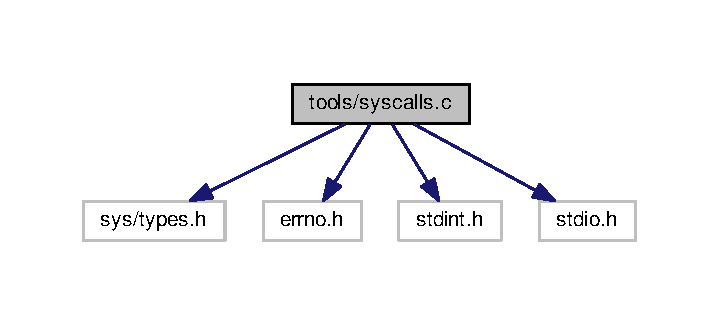
\includegraphics[width=345pt]{syscalls_8c__incl}
\end{center}
\end{figure}
\subsection*{Macros}
\begin{DoxyCompactItemize}
\item 
\hypertarget{group__newlib_gad72dbcf6d0153db1b8d8a58001feed83}{\#define {\bfseries D\+E\+B\+U\+G}~0}\label{group__newlib_gad72dbcf6d0153db1b8d8a58001feed83}

\item 
\hypertarget{group__newlib_ga1f464e950a4fa11e8821b5c725921a15}{\#define {\bfseries P\+R\+I\+N\+T\+F}(...)}\label{group__newlib_ga1f464e950a4fa11e8821b5c725921a15}

\end{DoxyCompactItemize}
\subsection*{Funções}
\begin{DoxyCompactItemize}
\item 
caddr\+\_\+t \hyperlink{group__newlib_gaae54d7b9578ba1fc171ce6f30f4c68a3}{\+\_\+sbrk} (int incr)
\begin{DoxyCompactList}\small\item\em Enlarges the allocated heap space. \end{DoxyCompactList}\end{DoxyCompactItemize}


\subsection{Descrição detalhada}
System calls. 


%--- End generated contents ---

% Index
\newpage
\phantomsection
\addcontentsline{toc}{chapter}{Índice}
\printindex

\end{document}
